% ----------------------------------------------------------------------------------------------------------
% Packages
% ----------------------------------------------------------------------------------------------------------

\documentclass[12pt,a4paper,bibliography=totocnumbered,listof=totocnumbered]{scrartcl}
\usepackage[english]{babel}
\usepackage[utf8]{inputenc}
\usepackage{amsmath}
\usepackage{amsfonts}
\usepackage{amssymb}
\usepackage{graphicx}
\usepackage{fancyhdr}
\usepackage{tabularx}
\usepackage{geometry}
\usepackage{setspace}
\usepackage[right]{eurosym}
\usepackage[printonlyused]{acronym}
\usepackage{subfig}
\usepackage{floatflt}
\usepackage[usenames,dvipsnames]{color}
\usepackage{colortbl}
\usepackage{paralist}
\usepackage{array}
\usepackage{titlesec}
%\usepackage{dsfont}
\usepackage{parskip}
\usepackage[right]{eurosym}
\usepackage[subfigure,titles]{tocloft}
\usepackage[pdfpagelabels=true]{hyperref}
\usepackage{mathdots}
\usepackage{listings}
\usepackage{lipsum}
\usepackage{booktabs}
\usepackage{fix-cm}
\usepackage{rotating}
\usepackage{pdflscape}
\usepackage{bbold}
\usepackage[labelfont=bf]{caption}
\captionsetup{labelfont=bf}
\usepackage{tikz}
\usepackage{breakcites}
\usepackage{float}
\usepackage{tcolorbox}
 \usepackage[flushleft]{threeparttable}
\usepackage{tocbibind}
\usepackage{algorithm2e}
\newcommand{\listofalgorithmes}{\tocfile{\listalgorithmcfname}{loa}}

%---------------------------------------------------------------------------------------------------------
% Packages
% ----------------------------------------------------------------------------------------------------------


\lstset{basicstyle=\footnotesize, captionpos=t, breaklines=true, showstringspaces=false, tabsize=2, frame=lines, numbers=left, numberstyle=\tiny, xleftmargin=2em, framexleftmargin=2em}
\makeatletter
\def\l@lstlisting#1#2{\@dottedtocline{1}{0em}{1em}{\hspace{1,5em} Lst. #1}{#2}}
\makeatother



\geometry{a4paper, top=27mm, left=27mm, right=27mm, bottom=35mm, headsep=10mm, footskip=12mm}

% ----------------------------------------------------------------------------------------------------------
% Packages
% ----------------------------------------------------------------------------------------------------------


\hypersetup{unicode=false, pdftoolbar=true, pdfmenubar=true, pdffitwindow=false, pdfstartview={FitH},
	pdftitle={Master Thesis},
	pdfauthor={Felix Gutmann},
	pdfsubject={Bachelor Thesis},
	pdfcreator={\LaTeX\ with package \flqq hyperref\frqq},
	pdfproducer={pdfTeX \the\pdftexversion.\pdftexrevision},
	pdfkeywords={Bachelor Thesis},
	pdfnewwindow=true,
	colorlinks=true,linkcolor=black,citecolor=black,filecolor=magenta,urlcolor=black}
\pdfinfo{/CreationDate (D:20110620133321)}
\DeclareMathOperator*{\argmin}{arg\,min}



\begin{document}

\titlespacing\section{0pt}{12pt plus 4pt minus 2pt}{0pt plus 2pt minus 2pt}
\titlespacing\subsection{0pt}{30pt plus 4pt minus 2pt}{0pt plus 2pt minus 2pt}
\titlespacing\subsubsection{0pt}{12pt plus 4pt minus 2pt}{0pt plus 2pt minus 2pt}
% Headers and footers

\renewcommand{\sectionmark}[1]{\markright{#1}}
\renewcommand{\leftmark}{\rightmark}
\pagestyle{fancy}
\lhead{}
\chead{}
\rhead{\thesection\space\contentsname}
%\lfoot{Complex Economic Systems - An analytical approach to Input-Output tables\newline}
\cfoot{}
\rfoot{\ \linebreak \thepage}
\renewcommand{\headrulewidth}{0.4pt}
\renewcommand{\footrulewidth}{0.4pt}

% ----------------------------------------------------------------------------------------------------------
%Prefix
% ----------------------------------------------------------------------------------------------------------

\renewcommand{\thesection}{\Roman{section}}
\renewcommand{\theHsection}{\Roman{section}}
\pagenumbering{Roman}

% ----------------------------------------------------------------------------------------------------------
% Title
% ----------------------------------------------------------------------------------------------------------

\thispagestyle{empty}
\begin{center}
	
\includegraphics[width=\textwidth]{Pictures/logo01.jpg}\\
	\vspace*{2cm}
	\vspace*{2cm}
	\Huge
	\textbf{Master Thesis}\\
	\vspace*{0.5cm}
	\large
	\textbf{Topic:}\\
	\vspace*{1cm}
	\textbf{Unsupervised learning in decision making}\\
	\vspace*{2cm}
\end{center}	

$\vspace{6cm}$
\begin{tabbing}
\hspace*{1cm}\=\hspace*{3.2cm}\=\hspace*{3cm}\=\hspace*{2.7cm}\= \kill
\onehalfspacing
\textbf{Author:} \>\> Domagoj Fizulic\\
\textbf{} \>\> Felix Gutmann\\
\textbf{Student number:} 	\>\> 125604\\
\textbf{} 	\>\> 125584\\
\textbf{Program:} \>\> M.S. Data Science\\
\textbf{E-Mail:} \>\> domagoj.fizulic@barcelonagse.eu\\
\textbf{} \>\> felix.gutmann@barcelonagse.eu
\end{tabbing}
\vspace{1cm}


\pagebreak
% ----------------------------------------------------------------------------------------------------------
% Abstract
% ----------------------------------------------------------------------------------------------------------


\onehalfspacing




\pagebreak

% ----------------------------------------------------------------------------------------------------------
% Index
% ----------------------------------------------------------------------------------------------------------


\renewcommand{\cfttabpresnum}{Tab. }
\renewcommand{\cftfigpresnum}{Fig. }
\settowidth{\cfttabnumwidth}{Fig. 10\quad}
\settowidth{\cftfignumwidth}{Fig. 10\quad}

\titlespacing{\section}{0pt}{12pt plus 4pt minus 2pt}{2pt plus 2pt minus 2pt}
\singlespacing
\rhead{Table of contents}
\renewcommand{\contentsname}{I Table of Contents}
\phantomsection
\addcontentsline{toc}{section}{\texorpdfstring{I \hspace{0.35em}Table of Contents}{Table of Contents}}
\addtocounter{section}{1}


% ----------------------------------------------------------------------------------------------------------
% Table of contents
% ----------------------------------------------------------------------------------------------------------

\setcounter{page}{1}

\rhead{Table of Contents}

	\tableofcontents


\pagebreak
% ----------------------------------------------------------------------------------------------------------
% List of figures
% ----------------------------------------------------------------------------------------------------------

\rhead{List of Figures}

	\listoffigures
	
	
\pagebreak
% ----------------------------------------------------------------------------------------------------------
% List of tables
% ----------------------------------------------------------------------------------------------------------

\rhead{List of Tables}

	\listoftables
	

\pagebreak
%----------------------------------------------------------------------------------------------------------
% List of Listings
% ----------------------------------------------------------------------------------------------------------

\rhead{List of Algorithms}
\listofalgorithmes
\pagebreak

%----------------------------------------------------------------------------------------------------------
% List of Symbols
% ---------------------------------------------------------------------------------------------------------

\renewcommand{\arraystretch}{1.5}	
\section{List of mathematical symbols}
\rhead{List of mathematical Symbols}

\begin{tabular}{p{6cm}p{9cm}}
\textbf{Symbol} 		& 		\textbf{Meaning} \\
\midrule
\vspace{0.3cm} & \vspace{0.3cm} 			\\
$\mu$ & Mean of bandits \\
$\sigma$ & Standard deviation of bandits \\
$a$				  & Action 	\\
$Q(a)$	& Value function for action $a$\\
$t$ & Discrete time step t \\
$R(a)$ & Reward for action $a$ \\
$\epsilon$			& Probability of exploration in epsilon greedy \\
$\alpha$ & Learning rate \\ 
$\eta$ & Same parameter as $\alpha$ sometimes used in cognitive science\\
$\tau$ & Softmax or temperature parameter \\
$\theta$ & Inverse temperature parameter \\
$X$ & Random variable \\
$H(X) $ &  Entropy of a  discrete random variable $X$ \\ 
$d(\cdot,\cdot)$ & Distance Function \\
$S(\cdot,\cdot)$ & Similarity Function \\
$K(\cdot,\cdot)$ & Kernel function \\
$m(\cdot,\cdot)$ & Matching function \\ 
$\Theta(\cdot)$ & Heavy side step function \\
$ \mathbb{R}_0^+$ & Positive real numbers including zero \\
$\mathcal{X}$ & Data set \\ 
\textbf{W} & Weighted adjacency matrix \\
$d_i$ & Degree of node $i$ \\
\textbf{D} & Diagonal matrix of degrees \\
\textbf{L} & Graph laplacian \\
\end{tabular}

\pagebreak

%----------------------------------------------------------------------------------------------------------
% List of abbreviations
% ---------------------------------------------------------------------------------------------------------

\section{List of abbreviations}
\rhead{List of Abbreviations}

\begin{tabular}{p{6cm}p{9cm}}
\textbf{Abbreviations} & \textbf{Description} 										\\
\midrule
\vspace{0.3cm} & \vspace{0.3cm} 														\\ 
IGT & Iowa gambling task \\
RL & Reinforcement learning \\
DTW & Dynamic time warp \\
EDR & Edit distance on real sequences \\
CH & Choices \\
BBC & Blockwise bad choices \\
ENT & Cumulative entropy \\
BENT & Blockwise entropy \\
CC & Concatenated \\
NMI & Normalized mutual information score \\
ARI & Adjusted rand index \\
VM & V-Measure score 
\end{tabular}

\newpage

% ----------------------------------------------------------------------------------------------------------
% Prefix 2
% ----------------------------------------------------------------------------------------------------------

% Title spacing

%\titlespacing{\section}{1cm}{12pt plus 4pt minus 2pt}{-6pt plus 2pt minus 2pt}
%\titlespacing{\subsection}{0pt}{12pt plus 4pt minus 2pt}{-6pt plus 2pt minus 2pt}
%\titlespacing{\subsubsection}{0pt}{12pt plus 4pt minus 2pt}{-6pt plus 2pt minus 2pt}

% Header

\renewcommand{\sectionmark}[1]{\markright{#1}}
\renewcommand{\subsectionmark}[1]{}
\renewcommand{\subsubsectionmark}[1]{}
\lhead{Chapter \thesection}
\rhead{\rightmark}

\onehalfspacing

\renewcommand{\thesection}{\arabic{section}}
\renewcommand{\theHsection}{\arabic{section}}
\setcounter{section}{0}
\pagenumbering{arabic}
\setcounter{page}{1}

%RGB Colour set

\definecolor{persblue}{rgb}{0.0862745,0.211765,0.360784}
\definecolor{persred}{rgb}{0.388235,0.145098,0.137255}
\definecolor{persgray}{rgb}{0.501961,0.501961,0.501961}
\definecolor{persgreen}{rgb}{0.054902,0.411765,0.352941}

%---------------------------------------------------------------------------------------------------------
% 1. Introduction
%---------------------------------------------------------------------------------------------------------

\section{Introduction and conceptual approach}

Decision-making is a cognitive process of selecting an option from a set of possible alternatives based on certain criteria \cite{Wang2007}. When analysing decision-making as a continuous process of interaction with the environment, learning becomes an important aspect. Learning is a complex procedure and can be described and estimated through different parameters. The learning procedure can be affected by different social and psychological conditions. Due to their cognitive ability people should show different learning behaviour.\\

One of the popular experiments for analysing decision behaviour is the Iowa Gambling Task. The decision making process is studied by monitoring peoples sequential choices in a controlled experiment environment.\\

In \textit{supervised learning} data are predicted by training a classifier based on examples. The identity of observations in the training sample is known. This is used to connect patterns in the data with corresponding labels of observations. In contrast to that in \textit{unsupervised learning} we don't know the ground truth. The objective is to discover natural clustering behaviour in the data itself and group objects into subsets, such that objects in those subsets are more closely related to each other \cite[page 9 et. seqq.]{Murphy2012} and \cite[page 501 et. seqq.]{hastie}. A vast class of clustering algorithms based on different approaches are proposed in the literature (e.g. hierarchical and optimization based clustering). This paper investigates, whether such unsupervised learning techniques can be used in the context of human decision making process to identify latent grouping. The decision making process is studied by monitoring peoples sequential choices in a controlled experiment environments over time. Thus, this paper operates in the intersection of machine learning and cognitive science. To our knowledge this particular setting has not been studied before.\\
We approach our research in the following way. We first set up a reinforcement learning based simulation framework to study theoretical boundaries of several clustering techniques and when they are applicable.
 Subsequently, we test our chosen methods on several  real experimental data sets. Corresponding to our simulation framework we first apply clustering algorithms to data from controlled n-armed bandit experiment.\footnote{A detailed introduction is given in section \ref{reinf}} A widely used approach to study human decision making process is the \textit{Iowa gambling task}, where participants try maximize rewards by choosing cards from different decks with different reward structures.\footnote{There are existing several slightly different versions of test. \cite{Steingroever2015} provides a data collection for from several sources giving a broad overview of different variations of the test.} Two decks have distributions with negative expectations while two have positive. However, each deck has its own variance and a set of profits.  Within this framework we analyse two different data sets. First we study decision making behaviour from people with different criminal profiles. Furthermore, we use another data set from cocaine abusers.\\


The report has the following structure. In section two we provide a short overview on related literature in the field. Section three is dedicated to the theoretical foundation and the simulation. We first provide knowledge of reinforcement and line out our experiment design in more detail. This section also includes an overview of applied algorithms, similarity and distance concepts. A mathematical formulation of the applied algorithms, similarity measures and cluster evaluation techniques can be found in the appendix.\footnote{Since our data are fairly small we will not discuss complexity of the algorithms.} Finally, we study their simulation performance and try to identify parameter settings, where they are applicable.\\ 
The rest of paper is address clustering our experimental data. We keep the scope of this paper tight and thus there some questions have to be left open. Thus we dedicated another section to discussing some possible extensions. We close this paper with a final summary of our results.

%---------------------------------------------------------------------------------------------------------
% 2. Literature
%---------------------------------------------------------------------------------------------------------

\section{Relevant Literature}

There exists a rich literature in cognitive science on identifying different behavioural groups. As mentioned in the introduction a commonly applied tool by a lot of studies is the Iowa Gambling Task experiment. Within that framework it has been shown that individuals with pre-frontal brain damage and decision-making defects continue to choose disadvantageously even after they learned the optimal strategy \cite{Bechara1997}.\\
A broad overview on other various results in the field can be found in \cite{Steingroever2013}. Several studies identify especially specific drug-user groups, e.g. cocaine addicts \cite{Stout2004}, chronic cannabis users \cite{Fridberg2010}, heavy alcohol users(heavy drinkers) \cite{Gullo2011}. Furthermore, extensive set of research is focused around particular mental disabilities, e.g. Asperger's disorder \cite{Johnson2006}, psychopathic tendencies \cite{Blair2001}, bipolar disorder \cite{Brambilla2012}, schizophrenia \cite{Martino2007} pathological gambling disorder \cite{Cavedini2002}, attention-deficit-hyperactivity disorder \cite{NiritAgay2010}. Most popular reinforcement learning models for identifying behavioural differences between different disorders are Expectancy Valence model \cite{Busemeyer2002} and Prospect Valence Learning model \cite{Ahn2008}.

%---------------------------------------------------------------------------------------------------------
% 3. Simmulation
%---------------------------------------------------------------------------------------------------------

\section{Theoretical Background and simulation experiments}

This section is dedicated to a detailed outline of our analysis approach and the results of our simulation experiments. The data we are analysing are gathered by observing peoples decisions over time. Hence, our data set are in the form $N \times M$ data set, where a row $N$ is the number of individuals and $M$ is the number of trials in the experiments. The data for each individual can be seen as a categorical time series. In terms of modeling there are two challenges. Some algorithms relying for example on euclidean distance while others operating on similarities. On one hand we introduce how repress those data and introduce related distance and similarity concepts for the algorithms. The section has a rather qualitative character. The appendix provides in more detail a mathematical background to applied algorithms, distance concepts and related clustering evaluation techniques. 

\subsection{Experiment design and problem formulation}

Figure \ref{fig:flow} depicts our simulation experiment design.\footnote{We implemented related coding for this project mainly in python. The code can be found in our  \href{https://github.com/FelixGSE/Master-Project}{github} repository.} The objective is to obtain a set of sequential choices for a given parameter setting of an artificial agent. We first generate a set of rewards by sampling $n-$vectors from a normal distribution ("\textit{multi arm bandits}"). The agent processes those rewards by sequentially choosing from those options. We repeat this procedure for several parameter settings for the agents and keep track of those choices which will define our data set.

 \begin{figure}[H]
	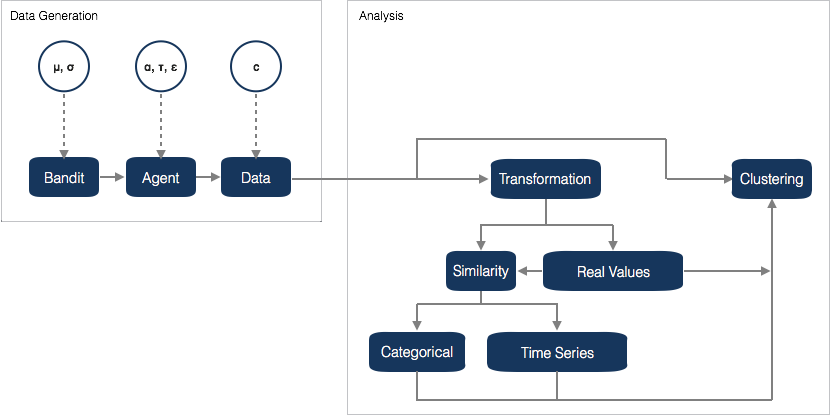
\includegraphics[width=\textwidth]{Pictures/flow01.png}
	\caption{Flowchart experiment design}
	\label{fig:flow}
\end{figure}

\subsection{Reinforcement Learning background and multi arm bandits}
\label{reinf}
Our simulation requires an artificial agent to produce desired data. The agent is relying \textit{Reinforcement Learning} (RL). Thus, we provide some necessary concepts of that field. The following definitions coming from \cite[chapter 1 and 2]{Sutton2012}. RL is a branch of \textit{machine learning} trying model the interaction of an artificial agents with its environment and the corresponding learning process. \\
In our particular setting the agent is confronted with the task of choosing sequentially from a set of $N$ possible choices. The agent doesn't have any knowledge about the system a priori. Therefore, it has to learn the nature of the system by continuously interacting with its environment while keeping track of the obtained information for each particular choice. Due to the lack of examples it has to explore different possible actions to identify the best action. Hence, it is useful to deviate from the current optimal strategy from time to time.\\ 
Each action in each step is associated with a given value based on the experience of the agent. This is modeled by defining a value function value function each action $a$. Denote the value function of an action $a$ as $Q(a)_t$. Hence the value function is defined average over the rewards for a given state. As mentioned it is necessary for the agent to explore its environment while simultaneously try to optimize its utility. Thus, a crucial task of the agent is to balance \textit{exploration} and \textit{exploitation} of the environment. There are two basic approaches to model this trade-off; An \textit{"Epsilon-Greedy"} action selection method and \textit{"Softmax"} selection method.\\
Within an epsilon greedy action selection strategy the next action is chosen based on the highest value function. However, to model exploration an random element is introduced to deviate from that greedy strategy with a certain probability (denoted by $\epsilon$). In general we can define the next action selected by the epsilon greedy strategy as:

\begin{flalign}
a_{t+1} = \begin{cases} 
\text{random action} & \text{, with probability } \epsilon \\
\arg \max_i Q(i)_t & \text{, with probability } 1-\epsilon
\end{cases} \nonumber
\end{flalign}

In the softmax action selection method each next action is sampled with a certain probability coming from a  \textit{Boltzmann Distribution)}. The probability for action a is computed by:

\begin{flalign}
P(a)_{t+1} = \frac{e^{\frac{Q_t(a)}{\tau}}}{\sum_{i}^{N} e^{\frac{Q_t(i)}{\tau}}}
\label{eq:softmax}
\end{flalign}

Using those probabilities for each action the next choice is sampled from this distribution. The softmax is essentially depending on the parameter $\tau$ parameter. It is controlling the how deterministic or random the agent is behaving. For increasing $\tau$ the numerator goes to one and the next action is therefore picked uniformly. For low values in $\tau$, actions with low value functions result in lower probabilities and hence in a greedy strategy. The parameter is sometimes called \textit{temparature}.\footnote{Another variation is to use the inverse of $\tau$ and denote it by $\theta$ (see, e.g. \cite{Stojic2015})}. 
After selecting an action the agent has to update its believes about it. The update rule is for the value function for an action is defined as:

\begin{flalign}
Q(a)_{t+1} = Q(a)_t + \alpha \left[ R(a)_t -  Q(a)_t	 \right], 
\label{eq:update}
\end{flalign}

where $\alpha$ is a is the non negative \textit{learning rate} defining how much the current action is affecting the believes and $R(a)_t$ is the reward of action a at step k. A challange might be how to initialize the value function. However, for convenience we set them to zero for all bandits. Those are the basic necessary ingredients to model artificial decision process. In the following we elaborate on further data processing.

\subsection{Data handling, unsupervised learning methods and similarities}
\label{algosim}
As mentioned we find two main challenges concerning the data. First, our data have a categorical nature. Furthermore, the learning process and corresponding behavioural changes also imposes changing dependence over time.\\
A well studied approach clustering such data types are \textit{hidden markov models}. For example, a decent study on that can be found in \cite{Pamminger2007}, \cite{Pamminger2009} and \cite{Pamminger2010a}. However, we focus our attention only on partition based clustering algorithms.\\
Some of the applied algorithms operate on distinct distance or similarity concepts. Given our data we  have to think carefully think about distance and similarity measures to respect the nature of our data and algorithms.\footnote{A formal definition of the distance and similarity can be found in the appendix} 
Furthermore, besides considering only raw choices we might try to re-express our data to discriminate them in different ways. 
One way is to apply \textit{Shannon's Entropy}  introduced by \cite{Shannon1948}. It is computed by using the empirical probability for each choices. For a discrete random variable  $X$ with probability $p$ the entropy is defined as \cite[page 32]{MacKay2005}:

\begin{flalign}
H(X) := -\sum_{i=1}^{N} p_i \log_2 p_i
\end{flalign}

Entropy gives measure on how random a random variable behaves.\footnote{From an applied perspective one get values for $X$ such that $p_i = 0$, we set $H(X) = 0$ for convenience  \cite[page 49]{Bishop2006}} Within the entropy framework we consider to types of entropies. For each time step we compute the entropy using choices done so far. We call this \textit{cumulative entropy}. Furthermore, we might want to observe more clearly how individuals adapt their behaviour over time. Considering an experiment with 100 trials we then compute the entropy for set of e.g. ten choices. We call this \textit{blockwise entropy}. Mapping choices to an entropy data set aims on discriminating individuals by their level randomness in their behaviour. \\
A second approach is based on the experimental setting. We know that within framework there are a set of choices, which are disadvantageous for the participant. Following e.g. \cite{Yechiam2008} or \cite{Ahn2008}, we then compute block wise the ratio of disadvantageous choices. We call this \textit{blockwise disadvantageous choice}. Finally we also consider a cumulative version of this ration, which we call \textit{cumulative disadvantageous choice}

Within our analysis we consider a broad selection of several clustering techniques and similarity concepts. Figure \ref{fig:cla} shows an overview of the algorithms and their corresponding distance/similarity requirements. A technical description for all of them is provided in the appendix. 

\begin{figure}[H]
	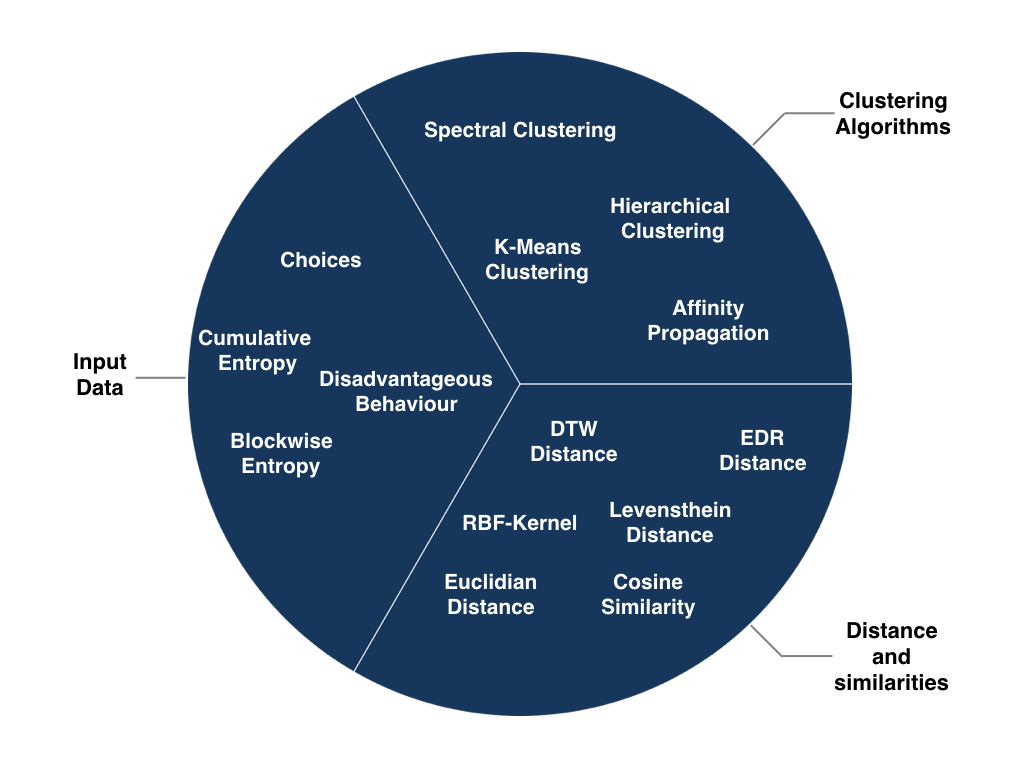
\includegraphics[width=\textwidth]{Pictures/DataClustering.jpeg}
	\caption{Input data, algorithms and proximity measures}
	\label{fig:cla}
\end{figure}

\subsection{Simulation setup and results}

We observed that that the clustering results of our simulation are fluctuating. Hence, to report stable results, the following numbers are computed as an average for each settings over 20 simulations. We also report the corresponding standard deviations to give an impression on the sensitivity of the clustering.\\

Our implementation is quite flexible. We can control both all parameters for each individual agent and their reward sets. We can control the number of trials for each agent and produce customized and multiple asymmetric cluster sizes. Furthermore, we can set prior values for each agent and each value function for the bandits. However, within our experiment we kept the settings simple. First we fix means and standard deviations for the bandits. Then first fix a value for alpha and run the simulations for different differences in tau. We repeat this procedure for fixed values of tau and vary alpha. Finally, we repeat this procedure with a different setting in the bandit means.\\
We are confronted with an enormous grid search over different parameters. Computing distances is very costly. As mentioned we have to run our simulations multiple times to get an impression of the variability. To keep the computation time to a reasonable we let the agents perform 100 trials and set the number of agents to 10 for each parameter setting. We ended up using solely the softmax function. The main reason for that decision is that we estimate those parameters later on for the experimental data.\\ 
The following table \ref{tab:simres}  shows a snippet of our simulation results. As described in the last section we have a broad range of similarity measures and algorithms. Therefore, we selected results in such a way, that we give an impression when clustering is working well. The results are selected in such a way, that they indicate the lower bound before clustering works perfectly. Naturally, we also found a lot of settings where clustering was not successful. A detailed overview on all numbers are given by tables \ref{tab:apstab1} to \ref{tab:apstab8} in the appendix.\footnote{To give an intuition about the numbers one can informally note that numbers below 0.200 - 0.300 do not show any really good clustering patterns.}
We find In general we find that our algorithms pick up the generated clusters when the differences in tau is sufficiently large. We tested this for different fixed values of $\alpha=\{0.1,0.5,1\}$. In general, we can say that if the difference in $\tau$ is larger than one, perfect clustering is possible and stable..\footnote{Standard deviation is equal to one} However, in some settings it also possible earlier.\footnote{See for example \ref{tab:apstab4} } \\
We repeated this procedure by fixing different values for $\tau$ and increase within each setting the values for $\alpha$. We are not able to achieve good clustering within that setting. In the summary table we listed an example, where we fix the difference in $\alpha$ to 0.9 and  still results are not very satisfying. Only if we fix the difference to 0.99 we are able to cluster within that setting.\\
Given the results we can conclude that we are able to discriminate individuals when their behaviour is significantly different with respect to randomness.\\
Concerning the data type the blockwise entropy seems to be overall the most successful one. In terms of algorithms we see that spectral clustering is in general outperforming the other algorithms. Furhtemore, the clustering results based on choices is constantly worse than the other data types.

\pagebreak

\begin{table}[!htbp] 
	\centering 
	\resizebox{\textwidth}{!}{\begin{tabular}{@{\extracolsep{0pt}} lllccccccccc} 
			\\[-1.8ex]\hline 
			\hline \\[-1.8ex] 
			& \textbf{Method} & \textbf{Similarity} & \textbf{Choices} & \textbf{Ratio disad. Choices}  & \textbf{Entropy}  & \textbf{Entropy Block} & \textbf{Concat} & \textbf{Normal. MI} & \textbf{Adj. Rand index} & \textbf{V-Measure} \\ 
			\hline 
			\textbf{Mu = \{0,2,4\}} &  &  &  &  &  &  &  &  &  &  \\ 
			\hline
			$\alpha$ = \{0.1\} & Spectral & RBF &  &  &  & x &  & 0.642 (0.200) & 0.653 (0.206) & 0.641 (0.200) \\ 
			$\tau$ = \{0.1, 0.7\} & Spectral & DTW &  &  & x &  &  & 0.580 (0.209) & 0.611 (0.205) & 0.580 (0.201) \\ 
			& K-Means & Euclidean &  &  &  &  & x & 0.382 (0.181) & 0.309 (0.237) & 0.381 (0.180) \\ 
			& Spectral & Levensthein & x &  &  &  &  & 0.350 (0.114) & 0.241 (0.163) & 0.347 (0.116) \\ 
			& Spectral & Euclidean &  & x &  &  &  & 0.306 (0.155) & 0.198 (0.179) & 0.303 (0.156) \\ 
			\hline
			\textbf{Average} &  &  &  &  &  &  &  & \textbf{0.367 (0.150)} &  \textbf{0.307 (0.195)} &  \textbf{0.364 (0.151)} \\ 
			\hline
			$\alpha$ = \{0.5\} & Spectral & DTW &  &  &  & x &  & 0.804 (0.212) & 0.804 (0.235) & 0.803 (0.213) \\ 
			$\tau$ = \{0.1, 1.0\} & Spectral & EDR &  &  & x &  &  & 0.652 (0.178) & 0.663 (0.203) & 0.652 (0.178) \\ 
			& Ward & Euclidean &  &  &  & x &  & 0.621 (0.208) & 0.596 (0.249) & 0.620 (0.209) \\ 
			& Spectral & Overlap & x &  &  &  &  & 0.599 (0.355) & 0.571 (0.406) & 0.597 (0.357) \\ 
			& K-Means & Euclidean &  &  &  & x &  & 0.562 (0.170) & 0.525 (0.220) & 0.562 (0.170) \\ 
			& Spectral & Levensthein & x &  &  &  &  & 0.368 (0.133) & 0.270 (0.169) & 0.366 (0.134) \\ 
			& K-Means & Euclidean & x &  &  &  &  & 0.275 (0.144) & 0.171 (0.147) & 0.272 (0.145) \\ 
			& K-Means & Euclidean &  &  &  &  & x & 0.399 (0.194)  & 0.338 (0.224) & 0.398 (0.194) \\ 
			& Spectral & Euclidean &  & x &  &  &  & 0.314 (0.109) & 0.197 (0.135) & 0.311 (0.110) \\ 
			\hline
			\textbf{Average} &  &  &  &  &  &  &  &   \textbf{0.408 (0.186)} &  \textbf{0.351 (0.217)} &  \textbf{0.406 (0.186)} \\ 
			\hline
			$\alpha$ = \{1.0\} & Spectral  & DTW &  &  &  & x &  & 0.792 (0.174) & 0.808 (0.170) & 0.792 (0.174) \\ 
			$\tau$ = \{0.1, 1.0\} &  Spectral  & EDR &  & x &  &  &  & 0.280 (0.198) & 0.201 (0.215) & 0.278 (0.198) \\ 
			& Spectral  & Levensthein & x &  &  &  &  & 0.276 (0.101) & 0.154 (0.113) & 0.272 (0.111) \\ 
			& Spectral  & EDR &  &  & x &  &  & 0.236 (0.196) & 0.171 (0.184) & 0.235 (0.195) \\ 
			& K-Means & Euclidean  &  &  &  &  & x & 0.099 (0.105) & 0.052 (0.097) & 0.098 (0.104) \\ 
			\hline
			\textbf{Average} &  &  &  &  &  &  &  &   \textbf{0.266 (0.203)} &  \textbf{0.204 (0.225)} &  \textbf{0.263 (0.204)} \\ 
			\hline
			\textbf{Mu = \{0,1,2\}} &  &  &  &  &  &  &  &  &  &  \\ 
			\hline
			$\alpha$ =  \{0.1\} & Spectral & DTW &  &  &  & x &  & 0.824 (0.166) & 0.837 (0.170) & 0.824 (0.166) \\ 
			$\tau$ = 	\{0.1, 0.5\} & Spectral & DTW &  &  & x &  &  & 0.636 (0.213) & 0.661 (0.205) & 0.636 (0.213) \\ 
			& K-Means & Euclidean &  &  &  &  & x & 0.532 (0.182) & 0.543 (0.206) & 0.531 (0.182) \\ 
			& Spectral & Levensthein & x &  &  &  &  & 0.411 (0.125) & 0.333 (0.160) & 0.410 (0.127) \\ 
			& Spectral & Euclidean &  & x &  &  &  & 0.242 (0.163) & 0.132 (0.187) & 0.238 (0.165) \\ 
			\hline
			\textbf{Average} &  &  &  &  &  &  &  &  \textbf{0.394 (0.210)} &  \textbf{0.338 (0.257)} &  \textbf{0.391 (0.212)} \\ 
			\hline
			$\alpha$ = \{0.5\} & Spectral & DTW &  &  &  & x &  & 0.769 (0.179) & 0.783 (0.185) & 0.769 (0.179) \\ 
			$\tau$ =  \{0.1, 0.5\} & Spectral & EDR &  & x &  &  &  & 0.335 (0.172) & 0.252 (0.191) & 0.333 (0.174) \\ 
			& Spectral & Levensthein & x &  &  &  &  & 0.324 (0.116) & 0.213 (0.128) & 0.322 (0.117) \\ 
			& Spectral & EDR &  &  & x &  &  & 0.221 (0.182) & 0.149 (0.161) & 0.221 (0.181) \\ 
			& K-Means & Euclidean &  &  &  &  & x & 0.137 (0.137) & 0.110 (0.152) & 0.136 (0.137) \\ 
			\hline
			\textbf{Average}  &  &  &  &  &  &  &  &  \textbf{0.248 (0.202)} &  \textbf{0.196 (0.212)} &  \textbf{0.246 (0.203)} \\ 
			\hline
			$\alpha$ = \{1.0\} & Spectral & DTW &  &  &  & x &  & 0.618 (0.192) & 0.627 (0.201) & 0.617 (0.192) \\ 
			$\tau$ = \{0.1, 0.7\} & Spectral & Levensthein & x &  &  &  &  & 0.252 (0.137) & 0.163 (0.147) & 0.249 (0.137) \\ 
			& Spectral & RBF &  &  & x &  &  & 0.215 (0.158) & 0.207 (0.188) & 0.215 (0.157) \\ 
			& Spectral & DTW &  & x &  &  &  & 0.205 (0.218) & 0.192 (0.247) & 0.205 (0.218) \\ 
			& K-Means & Euclidean &  &  &  &  & x & 0.185 (0.205) & 0.165 (0.225) & 0.185 (0.205) \\ 
			\hline
			\textbf{Average} &  &  &  &  &  &  &  &  \textbf{0.248 (0.183)} &  \textbf{0.220 (0.213)} &  \textbf{0.246 (0.184)} \\ 
			\hline
			\textbf{Mu = \{0,2,4\}}\tnote{*} &  &  &  &  &  &  &  &  &  &  \\ 
			\hline
			$\tau$ = \{1.0\}  & Spectral & DTW &  &  &  & x &  & 0.300 (0.232) & 0.273 (0.254) & 0.299 (0.232) \\ 
			$\alpha$ = \{0.1,0.9\} & Spectral & Cosine &  & x &  &  &  & 0.211 (0.158) & 0.159 (0.160) & 0.210 (0.158) \\ 
			& Spectral & Cosine &  &  & x &  &  & 0.191 (0.117) & 0.137 (0.127) & 0.189 (0.118) \\ 
			& Spectral & Cosine & x &  &  &  &  & 0.164 (0.110) & 0.115 (0.109) & 0.162 (0.109) \\ 
			& K-Means & Euclidean &  &  &  &  & x & 0.138 (0.153) & 0.091 (0.176) & 0.137 (0.153) \\ 
			\hline
			\textbf{Average}  &  &  &  &  &  &  &  &  \textbf{0.145 (0.067)} &  \textbf{0.101 (0.075)} &  \textbf{0.143 (0.067)} \\ 
			\hline \\[-1.8ex] 
		\end{tabular}}
		\begin{tcolorbox}[arc=0mm,title=Notes,boxrule=0.2mm,colbacktitle=white,coltitle=black,colback=white,top=0mm,bottom=0.1mm]
			\begin{tablenotes}
				\item The tables shows something
				\item[*] Selected result for fixed $\tau$ and varying and different $\alpha$
			\end{tablenotes}
		\end{tcolorbox}
		\caption{Selected simulation results}
		\label{tab:simres} 
	\end{table}


%---------------------------------------------------------------------------------------------------------
% 4. Data
%---------------------------------------------------------------------------------------------------------

\section{Data Analysis}

Our simulation results suggested that we can cluster the decision behaviour under some given constraints. In the following we apply our methods to three different real experiment datasets. As mentioned in the introduction the Iowa gambling task is popular way to monitor decision and learning process of individuals. In the simulation setting we initially define participants with a certain set of parameters. There are several techniques for estimating these parameters from the actual data, the most popular one being the expectancy valence model. 

\subsection{Multi-arm bandit experiment data}

The first data set is related to \cite{Stojic2015}. The data is gathered in a 20-arm bandits online experiment, in which users were compensated with small amount of money in exchange. Four different distributional settings were given to different people. In total the data sets consists of 429 participants divided in 199 female and 229 male participants.\footnote{One did not wish to answer} The average age 33.04 with standard deviation 11.75. Furthermore, the participants overall have a stronger higher education background. 261 participants have college degree, 39 a graduate degree and PhD respectively. 127 have a high school degree and 2 declined to answer.\\
We tried to identify different clusterings according to those demographics within those four sub experiments. Our results do not show worth mentioning clustering across mentioned demographics.\\
We try to discover clustering in the data. Within our simulation we set parameters, which classify individual subjects. Using the experimental data we come from the other way. The reinforcement learning model is quite closely related to the expectancy valence model from cognitive science. Referring to equation \eqref{eq:softmax} and equation \eqref{eq:update} we can try to recover the parameters by optimising those function based on the observed choices.

Two out of four experiments that we further analyse are 20-armed bandit gambling experiments. They differ by the level of noise of each arm and therefore the amount of reward distribution overlap.

We maximised the likelihood of the observed choice sequences in order to estimate alpha and tau for each individual in the dataset. This is a simplified version of the expectancy valence model as we do not estimate \textit{attention to gains} parameter. In our setting, the individuals are described in a two-dimensional space, as shown in plots below.

We continue by running our unsupervised learning models on the choice sequences and its by-products: entropy and bad choice sequences. Initially we hoped to achieve the same two-dimensional clusters given by the EV model, but this is not something we observed. However, some unsupervised models were linear and non-linear combinations of inverse tau and alpha that were correlated with different behaviours observed in the experiment. Top two graphs visualize alpha and inverse tau likelihood estimates of individuals in the high-noise experiment. The colours and shapes represent cluster labels produced by our unsupervised models. The top left graph shows one of the best two-cluster models. One could quite successfully draw an almost horizontal linear separator. This coincides with our simulation results where we observe that tau is more significant parameter of behaviour. Furthermore, one could fit a low order polynomial separator the would fit the labels almost perfectly. The top right graph follows the same argument as one could quite successfully fit two parallel almost horizontal separators. Same as in the previous graph, better clustering would be achieved by separators taking the convex form and being stacked in a non-crossing arrangement. Notice that in all four graphs the clustering fails as alpha estimator approaches zero. This was also observed in our simulation when setting alpha close to zero.

bottom graph version 1


Two bottom graphs represent data from the low noise experiment. We can see the average tau-inverse is higher which represents less randomization by the individuals. This is not surprising as due to lower noise, individuals can more easily differentiate gains between different choices and hence need to explore less. We may deduce that in the low-noise scenario alpha plays a stronger role as it is not possible to fit a satisfying horizontal linear separator. Following the same approach as in the first two graphs, the clustering can be improved by using convex separators.


bottom graph version 2


\begin{figure}[H]
	\centering
	\small
	\hspace*{-0.7in}
	\begin{tabular}{cc}
		% Created by tikzDevice version 0.10.1 on 2016-06-29 14:17:03
% !TEX encoding = UTF-8 Unicode
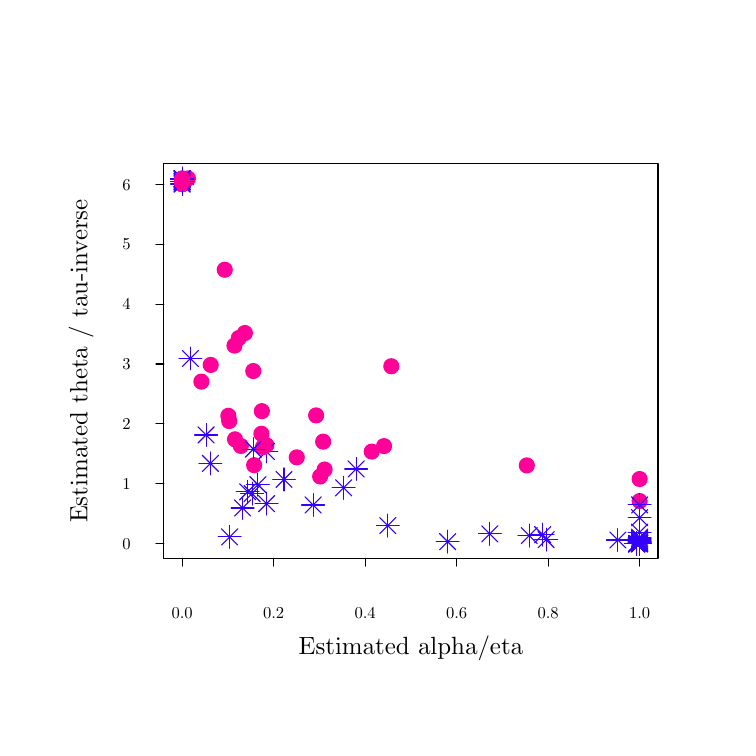
\begin{tikzpicture}[x=1pt,y=1pt]
\definecolor{fillColor}{RGB}{255,255,255}
\path[use as bounding box,fill=fillColor,fill opacity=0.00] (0,0) rectangle (252.94,252.94);
\begin{scope}
\path[clip] ( 49.20, 61.20) rectangle (227.75,203.75);
\definecolor{drawColor}{RGB}{51,0,255}

\path[draw=drawColor,line width= 0.4pt,line join=round,line cap=round] (218.21, 67.70) -- (224.06, 73.55);

\path[draw=drawColor,line width= 0.4pt,line join=round,line cap=round] (218.21, 73.55) -- (224.06, 67.70);

\path[draw=drawColor,line width= 0.4pt,line join=round,line cap=round] (216.99, 70.63) -- (225.27, 70.63);

\path[draw=drawColor,line width= 0.4pt,line join=round,line cap=round] (221.13, 66.49) -- (221.13, 74.77);

\path[draw=drawColor,line width= 0.4pt,line join=round,line cap=round] (218.21, 64.53) -- (224.06, 70.38);

\path[draw=drawColor,line width= 0.4pt,line join=round,line cap=round] (218.21, 70.38) -- (224.06, 64.53);

\path[draw=drawColor,line width= 0.4pt,line join=round,line cap=round] (217.00, 67.46) -- (225.27, 67.46);

\path[draw=drawColor,line width= 0.4pt,line join=round,line cap=round] (221.13, 63.32) -- (221.13, 71.59);

\path[draw=drawColor,line width= 0.4pt,line join=round,line cap=round] (217.14, 63.55) -- (222.99, 69.40);

\path[draw=drawColor,line width= 0.4pt,line join=round,line cap=round] (217.14, 69.40) -- (222.99, 63.55);

\path[draw=drawColor,line width= 0.4pt,line join=round,line cap=round] (215.93, 66.48) -- (224.21, 66.48);

\path[draw=drawColor,line width= 0.4pt,line join=round,line cap=round] (220.07, 62.34) -- (220.07, 70.62);
\definecolor{fillColor}{RGB}{255,0,153}

\path[fill=fillColor] ( 55.81,196.36) circle (  2.92);

\path[draw=drawColor,line width= 0.4pt,line join=round,line cap=round] ( 52.89,193.48) -- ( 58.74,199.33);

\path[draw=drawColor,line width= 0.4pt,line join=round,line cap=round] ( 52.89,199.33) -- ( 58.74,193.48);

\path[draw=drawColor,line width= 0.4pt,line join=round,line cap=round] ( 51.68,196.40) -- ( 59.95,196.40);

\path[draw=drawColor,line width= 0.4pt,line join=round,line cap=round] ( 55.81,192.27) -- ( 55.81,200.54);

\path[fill=fillColor] (221.13, 81.89) circle (  2.92);

\path[fill=fillColor] ( 55.81,197.86) circle (  2.92);

\path[fill=fillColor] ( 55.81,197.47) circle (  2.92);

\path[fill=fillColor] ( 55.81,197.08) circle (  2.92);

\path[fill=fillColor] ( 77.02,101.80) circle (  2.92);

\path[fill=fillColor] ( 78.50,142.61) circle (  2.92);

\path[draw=drawColor,line width= 0.4pt,line join=round,line cap=round] ( 52.89,195.14) -- ( 58.74,200.99);

\path[draw=drawColor,line width= 0.4pt,line join=round,line cap=round] ( 52.89,200.99) -- ( 58.74,195.14);

\path[draw=drawColor,line width= 0.4pt,line join=round,line cap=round] ( 51.68,198.07) -- ( 59.95,198.07);

\path[draw=drawColor,line width= 0.4pt,line join=round,line cap=round] ( 55.81,193.93) -- ( 55.81,202.20);

\path[fill=fillColor] (221.13, 89.84) circle (  2.92);

\path[draw=drawColor,line width= 0.4pt,line join=round,line cap=round] (184.42, 65.01) -- (190.27, 70.86);

\path[draw=drawColor,line width= 0.4pt,line join=round,line cap=round] (184.42, 70.86) -- (190.27, 65.01);

\path[draw=drawColor,line width= 0.4pt,line join=round,line cap=round] (183.21, 67.94) -- (191.49, 67.94);

\path[draw=drawColor,line width= 0.4pt,line join=round,line cap=round] (187.35, 63.80) -- (187.35, 72.07);

\path[fill=fillColor] ( 84.62,114.37) circle (  2.92);

\path[fill=fillColor] (106.77,103.34) circle (  2.92);

\path[fill=fillColor] (107.29, 93.27) circle (  2.92);

\path[fill=fillColor] ( 55.81,196.52) circle (  2.92);

\path[fill=fillColor] ( 86.26,102.07) circle (  2.92);

\path[draw=drawColor,line width= 0.4pt,line join=round,line cap=round] (218.21, 64.28) -- (224.06, 70.13);

\path[draw=drawColor,line width= 0.4pt,line join=round,line cap=round] (218.21, 70.13) -- (224.06, 64.28);

\path[draw=drawColor,line width= 0.4pt,line join=round,line cap=round] (217.00, 67.20) -- (225.27, 67.20);

\path[draw=drawColor,line width= 0.4pt,line join=round,line cap=round] (221.13, 63.07) -- (221.13, 71.34);

\path[draw=drawColor,line width= 0.4pt,line join=round,line cap=round] (218.09, 63.55) -- (223.94, 69.40);

\path[draw=drawColor,line width= 0.4pt,line join=round,line cap=round] (218.09, 69.40) -- (223.94, 63.55);

\path[draw=drawColor,line width= 0.4pt,line join=round,line cap=round] (216.88, 66.48) -- (225.15, 66.48);

\path[draw=drawColor,line width= 0.4pt,line join=round,line cap=round] (221.01, 62.34) -- (221.01, 70.62);

\path[draw=drawColor,line width= 0.4pt,line join=round,line cap=round] ( 89.70, 86.76) -- ( 95.55, 92.61);

\path[draw=drawColor,line width= 0.4pt,line join=round,line cap=round] ( 89.70, 92.61) -- ( 95.55, 86.76);

\path[draw=drawColor,line width= 0.4pt,line join=round,line cap=round] ( 88.49, 89.69) -- ( 96.76, 89.69);

\path[draw=drawColor,line width= 0.4pt,line join=round,line cap=round] ( 92.63, 85.55) -- ( 92.63, 93.82);

\path[draw=drawColor,line width= 0.4pt,line join=round,line cap=round] (148.84, 64.28) -- (154.69, 70.13);

\path[draw=drawColor,line width= 0.4pt,line join=round,line cap=round] (148.84, 70.13) -- (154.69, 64.28);

\path[draw=drawColor,line width= 0.4pt,line join=round,line cap=round] (147.63, 67.21) -- (155.90, 67.21);

\path[draw=drawColor,line width= 0.4pt,line join=round,line cap=round] (151.76, 63.07) -- (151.76, 71.34);

\path[draw=drawColor,line width= 0.4pt,line join=round,line cap=round] ( 52.89,194.35) -- ( 58.74,200.20);

\path[draw=drawColor,line width= 0.4pt,line join=round,line cap=round] ( 52.89,200.20) -- ( 58.74,194.35);

\path[draw=drawColor,line width= 0.4pt,line join=round,line cap=round] ( 51.68,197.28) -- ( 59.95,197.28);

\path[draw=drawColor,line width= 0.4pt,line join=round,line cap=round] ( 55.81,193.14) -- ( 55.81,201.41);

\path[draw=drawColor,line width= 0.4pt,line join=round,line cap=round] (218.09, 63.55) -- (223.94, 69.40);

\path[draw=drawColor,line width= 0.4pt,line join=round,line cap=round] (218.09, 69.40) -- (223.94, 63.55);

\path[draw=drawColor,line width= 0.4pt,line join=round,line cap=round] (216.88, 66.48) -- (225.15, 66.48);

\path[draw=drawColor,line width= 0.4pt,line join=round,line cap=round] (221.01, 62.34) -- (221.01, 70.62);

\path[fill=fillColor] (131.39,130.60) circle (  2.92);

\path[fill=fillColor] ( 62.76,125.04) circle (  2.92);

\path[draw=drawColor,line width= 0.4pt,line join=round,line cap=round] (217.14, 63.55) -- (222.99, 69.40);

\path[draw=drawColor,line width= 0.4pt,line join=round,line cap=round] (217.14, 69.40) -- (222.99, 63.55);

\path[draw=drawColor,line width= 0.4pt,line join=round,line cap=round] (215.93, 66.48) -- (224.21, 66.48);

\path[draw=drawColor,line width= 0.4pt,line join=round,line cap=round] (220.07, 62.34) -- (220.07, 70.62);

\path[draw=drawColor,line width= 0.4pt,line join=round,line cap=round] (100.20, 77.54) -- (106.05, 83.39);

\path[draw=drawColor,line width= 0.4pt,line join=round,line cap=round] (100.20, 83.39) -- (106.05, 77.54);

\path[draw=drawColor,line width= 0.4pt,line join=round,line cap=round] ( 98.99, 80.47) -- (107.27, 80.47);

\path[draw=drawColor,line width= 0.4pt,line join=round,line cap=round] (103.13, 76.33) -- (103.13, 84.60);

\path[draw=drawColor,line width= 0.4pt,line join=round,line cap=round] ( 83.30, 96.87) -- ( 89.15,102.72);

\path[draw=drawColor,line width= 0.4pt,line join=round,line cap=round] ( 83.30,102.72) -- ( 89.15, 96.87);

\path[draw=drawColor,line width= 0.4pt,line join=round,line cap=round] ( 82.09, 99.79) -- ( 90.36, 99.79);

\path[draw=drawColor,line width= 0.4pt,line join=round,line cap=round] ( 86.23, 95.66) -- ( 86.23,103.93);

\path[draw=drawColor,line width= 0.4pt,line join=round,line cap=round] (218.09, 63.55) -- (223.94, 69.40);

\path[draw=drawColor,line width= 0.4pt,line join=round,line cap=round] (218.09, 69.40) -- (223.94, 63.55);

\path[draw=drawColor,line width= 0.4pt,line join=round,line cap=round] (216.88, 66.48) -- (225.15, 66.48);

\path[draw=drawColor,line width= 0.4pt,line join=round,line cap=round] (221.01, 62.34) -- (221.01, 70.62);

\path[fill=fillColor] ( 97.23, 97.68) circle (  2.92);

\path[fill=fillColor] ( 72.52,112.69) circle (  2.92);

\path[draw=drawColor,line width= 0.4pt,line join=round,line cap=round] ( 52.89,194.28) -- ( 58.74,200.13);

\path[draw=drawColor,line width= 0.4pt,line join=round,line cap=round] ( 52.89,200.13) -- ( 58.74,194.28);

\path[draw=drawColor,line width= 0.4pt,line join=round,line cap=round] ( 51.68,197.20) -- ( 59.95,197.20);

\path[draw=drawColor,line width= 0.4pt,line join=round,line cap=round] ( 55.81,193.07) -- ( 55.81,201.34);

\path[draw=drawColor,line width= 0.4pt,line join=round,line cap=round] (218.21, 63.55) -- (224.06, 69.40);

\path[draw=drawColor,line width= 0.4pt,line join=round,line cap=round] (218.21, 69.40) -- (224.06, 63.55);

\path[draw=drawColor,line width= 0.4pt,line join=round,line cap=round] (217.00, 66.48) -- (225.27, 66.48);

\path[draw=drawColor,line width= 0.4pt,line join=round,line cap=round] (221.13, 62.34) -- (221.13, 70.62);

\path[fill=fillColor] ( 57.92,198.45) circle (  2.92);

\path[fill=fillColor] ( 85.02,101.38) circle (  2.92);

\path[fill=fillColor] ( 55.81,197.24) circle (  2.92);

\path[draw=drawColor,line width= 0.4pt,line join=round,line cap=round] ( 63.12, 92.55) -- ( 68.97, 98.40);

\path[draw=drawColor,line width= 0.4pt,line join=round,line cap=round] ( 63.12, 98.40) -- ( 68.97, 92.55);

\path[draw=drawColor,line width= 0.4pt,line join=round,line cap=round] ( 61.91, 95.47) -- ( 70.18, 95.47);

\path[draw=drawColor,line width= 0.4pt,line join=round,line cap=round] ( 66.04, 91.34) -- ( 66.04, 99.61);

\path[fill=fillColor] (105.68, 90.77) circle (  2.92);

\path[fill=fillColor] ( 55.81,196.40) circle (  2.92);

\path[draw=drawColor,line width= 0.4pt,line join=round,line cap=round] (217.14, 63.55) -- (222.99, 69.40);

\path[draw=drawColor,line width= 0.4pt,line join=round,line cap=round] (217.14, 69.40) -- (222.99, 63.55);

\path[draw=drawColor,line width= 0.4pt,line join=round,line cap=round] (215.93, 66.48) -- (224.21, 66.48);

\path[draw=drawColor,line width= 0.4pt,line join=round,line cap=round] (220.07, 62.34) -- (220.07, 70.62);

\path[fill=fillColor] ( 76.29,140.79) circle (  2.92);

\path[draw=drawColor,line width= 0.4pt,line join=round,line cap=round] ( 61.54,102.85) -- ( 67.39,108.70);

\path[draw=drawColor,line width= 0.4pt,line join=round,line cap=round] ( 61.54,108.70) -- ( 67.39,102.85);

\path[draw=drawColor,line width= 0.4pt,line join=round,line cap=round] ( 60.33,105.77) -- ( 68.60,105.77);

\path[draw=drawColor,line width= 0.4pt,line join=round,line cap=round] ( 64.47,101.64) -- ( 64.47,109.91);

\path[draw=drawColor,line width= 0.4pt,line join=round,line cap=round] (217.14, 63.55) -- (222.99, 69.40);

\path[draw=drawColor,line width= 0.4pt,line join=round,line cap=round] (217.14, 69.40) -- (222.99, 63.55);

\path[draw=drawColor,line width= 0.4pt,line join=round,line cap=round] (215.93, 66.48) -- (224.21, 66.48);

\path[draw=drawColor,line width= 0.4pt,line join=round,line cap=round] (220.07, 62.34) -- (220.07, 70.62);

\path[draw=drawColor,line width= 0.4pt,line join=round,line cap=round] (111.26, 83.75) -- (117.11, 89.60);

\path[draw=drawColor,line width= 0.4pt,line join=round,line cap=round] (111.26, 89.60) -- (117.11, 83.75);

\path[draw=drawColor,line width= 0.4pt,line join=round,line cap=round] (110.05, 86.68) -- (118.32, 86.68);

\path[draw=drawColor,line width= 0.4pt,line join=round,line cap=round] (114.19, 82.54) -- (114.19, 90.81);

\path[draw=drawColor,line width= 0.4pt,line join=round,line cap=round] ( 74.74, 76.46) -- ( 80.59, 82.31);

\path[draw=drawColor,line width= 0.4pt,line join=round,line cap=round] ( 74.74, 82.31) -- ( 80.59, 76.46);

\path[draw=drawColor,line width= 0.4pt,line join=round,line cap=round] ( 73.53, 79.39) -- ( 81.80, 79.39);

\path[draw=drawColor,line width= 0.4pt,line join=round,line cap=round] ( 77.67, 75.25) -- ( 77.67, 83.52);

\path[draw=drawColor,line width= 0.4pt,line join=round,line cap=round] ( 52.89,195.31) -- ( 58.74,201.16);

\path[draw=drawColor,line width= 0.4pt,line join=round,line cap=round] ( 52.89,201.16) -- ( 58.74,195.31);

\path[draw=drawColor,line width= 0.4pt,line join=round,line cap=round] ( 51.68,198.24) -- ( 59.95,198.24);

\path[draw=drawColor,line width= 0.4pt,line join=round,line cap=round] ( 55.81,194.10) -- ( 55.81,202.37);

\path[draw=drawColor,line width= 0.4pt,line join=round,line cap=round] (217.14, 63.55) -- (222.99, 69.40);

\path[draw=drawColor,line width= 0.4pt,line join=round,line cap=round] (217.14, 69.40) -- (222.99, 63.55);

\path[draw=drawColor,line width= 0.4pt,line join=round,line cap=round] (215.93, 66.48) -- (224.21, 66.48);

\path[draw=drawColor,line width= 0.4pt,line join=round,line cap=round] (220.07, 62.34) -- (220.07, 70.62);

\path[fill=fillColor] ( 55.81,197.55) circle (  2.92);

\path[fill=fillColor] ( 66.14,131.07) circle (  2.92);

\path[draw=drawColor,line width= 0.4pt,line join=round,line cap=round] ( 78.17, 81.66) -- ( 84.02, 87.51);

\path[draw=drawColor,line width= 0.4pt,line join=round,line cap=round] ( 78.17, 87.51) -- ( 84.02, 81.66);

\path[draw=drawColor,line width= 0.4pt,line join=round,line cap=round] ( 76.96, 84.59) -- ( 85.23, 84.59);

\path[draw=drawColor,line width= 0.4pt,line join=round,line cap=round] ( 81.10, 80.45) -- ( 81.10, 88.72);

\path[fill=fillColor] ( 55.81,198.47) circle (  2.92);

\path[draw=drawColor,line width= 0.4pt,line join=round,line cap=round] (178.32, 66.48) -- (184.17, 72.33);

\path[draw=drawColor,line width= 0.4pt,line join=round,line cap=round] (178.32, 72.33) -- (184.17, 66.48);

\path[draw=drawColor,line width= 0.4pt,line join=round,line cap=round] (177.11, 69.41) -- (185.38, 69.41);

\path[draw=drawColor,line width= 0.4pt,line join=round,line cap=round] (181.25, 65.27) -- (181.25, 73.54);

\path[fill=fillColor] ( 81.52,128.87) circle (  2.92);

\path[fill=fillColor] ( 71.21,165.47) circle (  2.92);

\path[draw=drawColor,line width= 0.4pt,line join=round,line cap=round] ( 52.89,194.34) -- ( 58.74,200.19);

\path[draw=drawColor,line width= 0.4pt,line join=round,line cap=round] ( 52.89,200.19) -- ( 58.74,194.34);

\path[draw=drawColor,line width= 0.4pt,line join=round,line cap=round] ( 51.68,197.27) -- ( 59.95,197.27);

\path[draw=drawColor,line width= 0.4pt,line join=round,line cap=round] ( 55.81,193.13) -- ( 55.81,201.40);

\path[draw=drawColor,line width= 0.4pt,line join=round,line cap=round] ( 52.89,195.48) -- ( 58.74,201.33);

\path[draw=drawColor,line width= 0.4pt,line join=round,line cap=round] ( 52.89,201.33) -- ( 58.74,195.48);

\path[draw=drawColor,line width= 0.4pt,line join=round,line cap=round] ( 51.68,198.41) -- ( 59.95,198.41);

\path[draw=drawColor,line width= 0.4pt,line join=round,line cap=round] ( 55.81,194.27) -- ( 55.81,202.55);

\path[draw=drawColor,line width= 0.4pt,line join=round,line cap=round] (218.21, 77.56) -- (224.06, 83.41);

\path[draw=drawColor,line width= 0.4pt,line join=round,line cap=round] (218.21, 83.41) -- (224.06, 77.56);

\path[draw=drawColor,line width= 0.4pt,line join=round,line cap=round] (217.00, 80.48) -- (225.27, 80.48);

\path[draw=drawColor,line width= 0.4pt,line join=round,line cap=round] (221.13, 76.35) -- (221.13, 84.62);

\path[draw=drawColor,line width= 0.4pt,line join=round,line cap=round] ( 76.56, 82.29) -- ( 82.41, 88.14);

\path[draw=drawColor,line width= 0.4pt,line join=round,line cap=round] ( 76.56, 88.14) -- ( 82.41, 82.29);

\path[draw=drawColor,line width= 0.4pt,line join=round,line cap=round] ( 75.35, 85.21) -- ( 83.62, 85.21);

\path[draw=drawColor,line width= 0.4pt,line join=round,line cap=round] ( 79.48, 81.08) -- ( 79.48, 89.35);

\path[draw=drawColor,line width= 0.4pt,line join=round,line cap=round] (218.21, 64.13) -- (224.06, 69.98);

\path[draw=drawColor,line width= 0.4pt,line join=round,line cap=round] (218.21, 69.98) -- (224.06, 64.13);

\path[draw=drawColor,line width= 0.4pt,line join=round,line cap=round] (217.00, 67.06) -- (225.27, 67.06);

\path[draw=drawColor,line width= 0.4pt,line join=round,line cap=round] (221.13, 62.92) -- (221.13, 71.19);

\path[fill=fillColor] ( 74.92,104.19) circle (  2.92);

\path[draw=drawColor,line width= 0.4pt,line join=round,line cap=round] (218.21, 63.55) -- (224.06, 69.40);

\path[draw=drawColor,line width= 0.4pt,line join=round,line cap=round] (218.21, 69.40) -- (224.06, 63.55);

\path[draw=drawColor,line width= 0.4pt,line join=round,line cap=round] (217.00, 66.48) -- (225.27, 66.48);

\path[draw=drawColor,line width= 0.4pt,line join=round,line cap=round] (221.13, 62.34) -- (221.13, 70.62);

\path[draw=drawColor,line width= 0.4pt,line join=round,line cap=round] ( 70.05, 65.99) -- ( 75.90, 71.84);

\path[draw=drawColor,line width= 0.4pt,line join=round,line cap=round] ( 70.05, 71.84) -- ( 75.90, 65.99);

\path[draw=drawColor,line width= 0.4pt,line join=round,line cap=round] ( 68.84, 68.92) -- ( 77.11, 68.92);

\path[draw=drawColor,line width= 0.4pt,line join=round,line cap=round] ( 72.98, 64.78) -- ( 72.98, 73.05);

\path[draw=drawColor,line width= 0.4pt,line join=round,line cap=round] ( 55.87,130.47) -- ( 61.72,136.32);

\path[draw=drawColor,line width= 0.4pt,line join=round,line cap=round] ( 55.87,136.32) -- ( 61.72,130.47);

\path[draw=drawColor,line width= 0.4pt,line join=round,line cap=round] ( 54.66,133.40) -- ( 62.93,133.40);

\path[draw=drawColor,line width= 0.4pt,line join=round,line cap=round] ( 58.79,129.26) -- ( 58.79,137.53);

\path[draw=drawColor,line width= 0.4pt,line join=round,line cap=round] (218.21, 65.12) -- (224.06, 70.97);

\path[draw=drawColor,line width= 0.4pt,line join=round,line cap=round] (218.21, 70.97) -- (224.06, 65.12);

\path[draw=drawColor,line width= 0.4pt,line join=round,line cap=round] (217.00, 68.05) -- (225.27, 68.05);

\path[draw=drawColor,line width= 0.4pt,line join=round,line cap=round] (221.13, 63.91) -- (221.13, 72.18);

\path[draw=drawColor,line width= 0.4pt,line join=round,line cap=round] ( 52.89,195.42) -- ( 58.74,201.27);

\path[draw=drawColor,line width= 0.4pt,line join=round,line cap=round] ( 52.89,201.27) -- ( 58.74,195.42);

\path[draw=drawColor,line width= 0.4pt,line join=round,line cap=round] ( 51.68,198.35) -- ( 59.95,198.35);

\path[draw=drawColor,line width= 0.4pt,line join=round,line cap=round] ( 55.81,194.21) -- ( 55.81,202.48);

\path[fill=fillColor] ( 84.46,106.19) circle (  2.92);

\path[draw=drawColor,line width= 0.4pt,line join=round,line cap=round] ( 80.27, 84.89) -- ( 86.12, 90.74);

\path[draw=drawColor,line width= 0.4pt,line join=round,line cap=round] ( 80.27, 90.74) -- ( 86.12, 84.89);

\path[draw=drawColor,line width= 0.4pt,line join=round,line cap=round] ( 79.06, 87.82) -- ( 87.33, 87.82);

\path[draw=drawColor,line width= 0.4pt,line join=round,line cap=round] ( 83.20, 83.68) -- ( 83.20, 91.95);

\path[draw=drawColor,line width= 0.4pt,line join=round,line cap=round] (127.20, 70.09) -- (133.05, 75.94);

\path[draw=drawColor,line width= 0.4pt,line join=round,line cap=round] (127.20, 75.94) -- (133.05, 70.09);

\path[draw=drawColor,line width= 0.4pt,line join=round,line cap=round] (125.99, 73.01) -- (134.26, 73.01);

\path[draw=drawColor,line width= 0.4pt,line join=round,line cap=round] (130.13, 68.88) -- (130.13, 77.15);

\path[draw=drawColor,line width= 0.4pt,line join=round,line cap=round] ( 83.40, 78.00) -- ( 89.25, 83.85);

\path[draw=drawColor,line width= 0.4pt,line join=round,line cap=round] ( 83.40, 83.85) -- ( 89.25, 78.00);

\path[draw=drawColor,line width= 0.4pt,line join=round,line cap=round] ( 82.18, 80.93) -- ( 90.46, 80.93);

\path[draw=drawColor,line width= 0.4pt,line join=round,line cap=round] ( 86.32, 76.79) -- ( 86.32, 85.06);

\path[draw=drawColor,line width= 0.4pt,line join=round,line cap=round] (217.14, 63.55) -- (222.99, 69.40);

\path[draw=drawColor,line width= 0.4pt,line join=round,line cap=round] (217.14, 69.40) -- (222.99, 63.55);

\path[draw=drawColor,line width= 0.4pt,line join=round,line cap=round] (215.93, 66.48) -- (224.21, 66.48);

\path[draw=drawColor,line width= 0.4pt,line join=round,line cap=round] (220.07, 62.34) -- (220.07, 70.62);

\path[draw=drawColor,line width= 0.4pt,line join=round,line cap=round] ( 52.89,195.45) -- ( 58.74,201.30);

\path[draw=drawColor,line width= 0.4pt,line join=round,line cap=round] ( 52.89,201.30) -- ( 58.74,195.45);

\path[draw=drawColor,line width= 0.4pt,line join=round,line cap=round] ( 51.68,198.37) -- ( 59.95,198.37);

\path[draw=drawColor,line width= 0.4pt,line join=round,line cap=round] ( 55.81,194.23) -- ( 55.81,202.51);

\path[draw=drawColor,line width= 0.4pt,line join=round,line cap=round] ( 52.89,194.59) -- ( 58.74,200.44);

\path[draw=drawColor,line width= 0.4pt,line join=round,line cap=round] ( 52.89,200.44) -- ( 58.74,194.59);

\path[draw=drawColor,line width= 0.4pt,line join=round,line cap=round] ( 51.68,197.51) -- ( 59.95,197.51);

\path[draw=drawColor,line width= 0.4pt,line join=round,line cap=round] ( 55.81,193.38) -- ( 55.81,201.65);

\path[fill=fillColor] ( 81.83, 94.84) circle (  2.92);

\path[fill=fillColor] ( 55.81,198.37) circle (  2.92);

\path[draw=drawColor,line width= 0.4pt,line join=round,line cap=round] ( 52.89,193.73) -- ( 58.74,199.58);

\path[draw=drawColor,line width= 0.4pt,line join=round,line cap=round] ( 52.89,199.58) -- ( 58.74,193.73);

\path[draw=drawColor,line width= 0.4pt,line join=round,line cap=round] ( 51.68,196.66) -- ( 59.95,196.66);

\path[draw=drawColor,line width= 0.4pt,line join=round,line cap=round] ( 55.81,192.52) -- ( 55.81,200.79);

\path[draw=drawColor,line width= 0.4pt,line join=round,line cap=round] (217.14, 63.55) -- (222.99, 69.40);

\path[draw=drawColor,line width= 0.4pt,line join=round,line cap=round] (217.14, 69.40) -- (222.99, 63.55);

\path[draw=drawColor,line width= 0.4pt,line join=round,line cap=round] (215.93, 66.48) -- (224.21, 66.48);

\path[draw=drawColor,line width= 0.4pt,line join=round,line cap=round] (220.07, 62.34) -- (220.07, 70.62);

\path[draw=drawColor,line width= 0.4pt,line join=round,line cap=round] (217.14, 63.55) -- (222.99, 69.40);

\path[draw=drawColor,line width= 0.4pt,line join=round,line cap=round] (217.14, 69.40) -- (222.99, 63.55);

\path[draw=drawColor,line width= 0.4pt,line join=round,line cap=round] (215.93, 66.48) -- (224.21, 66.48);

\path[draw=drawColor,line width= 0.4pt,line join=round,line cap=round] (220.07, 62.34) -- (220.07, 70.62);

\path[draw=drawColor,line width= 0.4pt,line join=round,line cap=round] (115.76, 90.55) -- (121.61, 96.40);

\path[draw=drawColor,line width= 0.4pt,line join=round,line cap=round] (115.76, 96.40) -- (121.61, 90.55);

\path[draw=drawColor,line width= 0.4pt,line join=round,line cap=round] (114.55, 93.48) -- (122.82, 93.48);

\path[draw=drawColor,line width= 0.4pt,line join=round,line cap=round] (118.68, 89.34) -- (118.68, 97.62);

\path[fill=fillColor] ( 74.73,138.05) circle (  2.92);

\path[draw=drawColor,line width= 0.4pt,line join=round,line cap=round] (217.14, 63.55) -- (222.99, 69.40);

\path[draw=drawColor,line width= 0.4pt,line join=round,line cap=round] (217.14, 69.40) -- (222.99, 63.55);

\path[draw=drawColor,line width= 0.4pt,line join=round,line cap=round] (215.93, 66.48) -- (224.21, 66.48);

\path[draw=drawColor,line width= 0.4pt,line join=round,line cap=round] (220.07, 62.34) -- (220.07, 70.62);

\path[fill=fillColor] (104.23,112.82) circle (  2.92);

\path[draw=drawColor,line width= 0.4pt,line join=round,line cap=round] (218.21, 63.55) -- (224.06, 69.40);

\path[draw=drawColor,line width= 0.4pt,line join=round,line cap=round] (218.21, 69.40) -- (224.06, 63.55);

\path[draw=drawColor,line width= 0.4pt,line join=round,line cap=round] (217.00, 66.48) -- (225.27, 66.48);

\path[draw=drawColor,line width= 0.4pt,line join=round,line cap=round] (221.13, 62.34) -- (221.13, 70.62);

\path[draw=drawColor,line width= 0.4pt,line join=round,line cap=round] (217.14, 63.55) -- (222.99, 69.40);

\path[draw=drawColor,line width= 0.4pt,line join=round,line cap=round] (217.14, 69.40) -- (222.99, 63.55);

\path[draw=drawColor,line width= 0.4pt,line join=round,line cap=round] (215.93, 66.48) -- (224.21, 66.48);

\path[draw=drawColor,line width= 0.4pt,line join=round,line cap=round] (220.07, 62.34) -- (220.07, 70.62);

\path[fill=fillColor] (124.32, 99.75) circle (  2.92);

\path[draw=drawColor,line width= 0.4pt,line join=round,line cap=round] (218.21, 63.55) -- (224.06, 69.40);

\path[draw=drawColor,line width= 0.4pt,line join=round,line cap=round] (218.21, 69.40) -- (224.06, 63.55);

\path[draw=drawColor,line width= 0.4pt,line join=round,line cap=round] (217.00, 66.48) -- (225.27, 66.48);

\path[draw=drawColor,line width= 0.4pt,line join=round,line cap=round] (221.13, 62.34) -- (221.13, 70.62);

\path[fill=fillColor] ( 55.81,198.10) circle (  2.92);

\path[fill=fillColor] ( 72.82,110.80) circle (  2.92);

\path[draw=drawColor,line width= 0.4pt,line join=round,line cap=round] (217.14, 63.55) -- (222.99, 69.40);

\path[draw=drawColor,line width= 0.4pt,line join=round,line cap=round] (217.14, 69.40) -- (222.99, 63.55);

\path[draw=drawColor,line width= 0.4pt,line join=round,line cap=round] (215.93, 66.48) -- (224.21, 66.48);

\path[draw=drawColor,line width= 0.4pt,line join=round,line cap=round] (220.07, 62.34) -- (220.07, 70.62);

\path[draw=drawColor,line width= 0.4pt,line join=round,line cap=round] (164.06, 67.09) -- (169.91, 72.94);

\path[draw=drawColor,line width= 0.4pt,line join=round,line cap=round] (164.06, 72.94) -- (169.91, 67.09);

\path[draw=drawColor,line width= 0.4pt,line join=round,line cap=round] (162.85, 70.02) -- (171.12, 70.02);

\path[draw=drawColor,line width= 0.4pt,line join=round,line cap=round] (166.99, 65.88) -- (166.99, 74.15);

\path[fill=fillColor] (128.76,101.74) circle (  2.92);

\path[draw=drawColor,line width= 0.4pt,line join=round,line cap=round] ( 78.63, 97.72) -- ( 84.48,103.57);

\path[draw=drawColor,line width= 0.4pt,line join=round,line cap=round] ( 78.63,103.57) -- ( 84.48, 97.72);

\path[draw=drawColor,line width= 0.4pt,line join=round,line cap=round] ( 77.42,100.64) -- ( 85.69,100.64);

\path[draw=drawColor,line width= 0.4pt,line join=round,line cap=round] ( 81.56, 96.51) -- ( 81.56,104.78);

\path[draw=drawColor,line width= 0.4pt,line join=round,line cap=round] (218.21, 65.39) -- (224.06, 71.24);

\path[draw=drawColor,line width= 0.4pt,line join=round,line cap=round] (218.21, 71.24) -- (224.06, 65.39);

\path[draw=drawColor,line width= 0.4pt,line join=round,line cap=round] (217.00, 68.32) -- (225.27, 68.32);

\path[draw=drawColor,line width= 0.4pt,line join=round,line cap=round] (221.13, 64.18) -- (221.13, 72.46);

\path[draw=drawColor,line width= 0.4pt,line join=round,line cap=round] (217.14, 63.55) -- (222.99, 69.40);

\path[draw=drawColor,line width= 0.4pt,line join=round,line cap=round] (217.14, 69.40) -- (222.99, 63.55);

\path[draw=drawColor,line width= 0.4pt,line join=round,line cap=round] (215.93, 66.48) -- (224.21, 66.48);

\path[draw=drawColor,line width= 0.4pt,line join=round,line cap=round] (220.07, 62.34) -- (220.07, 70.62);

\path[draw=drawColor,line width= 0.4pt,line join=round,line cap=round] (218.21, 72.94) -- (224.06, 78.79);

\path[draw=drawColor,line width= 0.4pt,line join=round,line cap=round] (218.21, 78.79) -- (224.06, 72.94);

\path[draw=drawColor,line width= 0.4pt,line join=round,line cap=round] (217.00, 75.87) -- (225.27, 75.87);

\path[draw=drawColor,line width= 0.4pt,line join=round,line cap=round] (221.13, 71.73) -- (221.13, 80.00);

\path[draw=drawColor,line width= 0.4pt,line join=round,line cap=round] (210.35, 64.88) -- (216.20, 70.73);

\path[draw=drawColor,line width= 0.4pt,line join=round,line cap=round] (210.35, 70.73) -- (216.20, 64.88);

\path[draw=drawColor,line width= 0.4pt,line join=round,line cap=round] (209.14, 67.81) -- (217.41, 67.81);

\path[draw=drawColor,line width= 0.4pt,line join=round,line cap=round] (213.27, 63.67) -- (213.27, 71.94);

\path[fill=fillColor] ( 55.81,197.65) circle (  2.92);

\path[draw=drawColor,line width= 0.4pt,line join=round,line cap=round] (218.20, 63.89) -- (224.05, 69.74);

\path[draw=drawColor,line width= 0.4pt,line join=round,line cap=round] (218.20, 69.74) -- (224.05, 63.89);

\path[draw=drawColor,line width= 0.4pt,line join=round,line cap=round] (216.99, 66.82) -- (225.26, 66.82);

\path[draw=drawColor,line width= 0.4pt,line join=round,line cap=round] (221.13, 62.68) -- (221.13, 70.95);

\path[draw=drawColor,line width= 0.4pt,line join=round,line cap=round] (217.14, 63.55) -- (222.99, 69.40);

\path[draw=drawColor,line width= 0.4pt,line join=round,line cap=round] (217.14, 69.40) -- (222.99, 63.55);

\path[draw=drawColor,line width= 0.4pt,line join=round,line cap=round] (215.93, 66.48) -- (224.21, 66.48);

\path[draw=drawColor,line width= 0.4pt,line join=round,line cap=round] (220.07, 62.34) -- (220.07, 70.62);

\path[draw=drawColor,line width= 0.4pt,line join=round,line cap=round] (218.21, 65.90) -- (224.06, 71.75);

\path[draw=drawColor,line width= 0.4pt,line join=round,line cap=round] (218.21, 71.75) -- (224.06, 65.90);

\path[draw=drawColor,line width= 0.4pt,line join=round,line cap=round] (217.00, 68.83) -- (225.27, 68.83);

\path[draw=drawColor,line width= 0.4pt,line join=round,line cap=round] (221.13, 64.69) -- (221.13, 72.97);

\path[draw=drawColor,line width= 0.4pt,line join=round,line cap=round] (183.17, 66.80) -- (189.02, 72.65);

\path[draw=drawColor,line width= 0.4pt,line join=round,line cap=round] (183.17, 72.65) -- (189.02, 66.80);

\path[draw=drawColor,line width= 0.4pt,line join=round,line cap=round] (181.96, 69.72) -- (190.23, 69.72);

\path[draw=drawColor,line width= 0.4pt,line join=round,line cap=round] (186.10, 65.59) -- (186.10, 73.86);

\path[fill=fillColor] ( 55.81,197.02) circle (  2.92);

\path[fill=fillColor] (180.36, 94.76) circle (  2.92);
\end{scope}
\begin{scope}
\path[clip] (  0.00,  0.00) rectangle (252.94,252.94);
\definecolor{drawColor}{RGB}{0,0,0}

\path[draw=drawColor,line width= 0.4pt,line join=round,line cap=round] ( 55.81, 61.20) -- (221.13, 61.20);

\path[draw=drawColor,line width= 0.4pt,line join=round,line cap=round] ( 55.81, 61.20) -- ( 55.81, 58.35);

\path[draw=drawColor,line width= 0.4pt,line join=round,line cap=round] ( 88.88, 61.20) -- ( 88.88, 58.35);

\path[draw=drawColor,line width= 0.4pt,line join=round,line cap=round] (121.94, 61.20) -- (121.94, 58.35);

\path[draw=drawColor,line width= 0.4pt,line join=round,line cap=round] (155.00, 61.20) -- (155.00, 58.35);

\path[draw=drawColor,line width= 0.4pt,line join=round,line cap=round] (188.07, 61.20) -- (188.07, 58.35);

\path[draw=drawColor,line width= 0.4pt,line join=round,line cap=round] (221.13, 61.20) -- (221.13, 58.35);

\node[text=drawColor,anchor=base,inner sep=0pt, outer sep=0pt, scale=  0.60] at ( 55.81, 39.60) {0.0};

\node[text=drawColor,anchor=base,inner sep=0pt, outer sep=0pt, scale=  0.60] at ( 88.88, 39.60) {0.2};

\node[text=drawColor,anchor=base,inner sep=0pt, outer sep=0pt, scale=  0.60] at (121.94, 39.60) {0.4};

\node[text=drawColor,anchor=base,inner sep=0pt, outer sep=0pt, scale=  0.60] at (155.00, 39.60) {0.6};

\node[text=drawColor,anchor=base,inner sep=0pt, outer sep=0pt, scale=  0.60] at (188.07, 39.60) {0.8};

\node[text=drawColor,anchor=base,inner sep=0pt, outer sep=0pt, scale=  0.60] at (221.13, 39.60) {1.0};

\path[draw=drawColor,line width= 0.4pt,line join=round,line cap=round] ( 49.20, 66.48) -- ( 49.20,196.32);

\path[draw=drawColor,line width= 0.4pt,line join=round,line cap=round] ( 49.20, 66.48) -- ( 46.35, 66.48);

\path[draw=drawColor,line width= 0.4pt,line join=round,line cap=round] ( 49.20, 88.12) -- ( 46.35, 88.12);

\path[draw=drawColor,line width= 0.4pt,line join=round,line cap=round] ( 49.20,109.76) -- ( 46.35,109.76);

\path[draw=drawColor,line width= 0.4pt,line join=round,line cap=round] ( 49.20,131.40) -- ( 46.35,131.40);

\path[draw=drawColor,line width= 0.4pt,line join=round,line cap=round] ( 49.20,153.04) -- ( 46.35,153.04);

\path[draw=drawColor,line width= 0.4pt,line join=round,line cap=round] ( 49.20,174.68) -- ( 46.35,174.68);

\path[draw=drawColor,line width= 0.4pt,line join=round,line cap=round] ( 49.20,196.32) -- ( 46.35,196.32);

\node[text=drawColor,anchor=base east,inner sep=0pt, outer sep=0pt, scale=  0.60] at ( 37.20, 64.41) {0};

\node[text=drawColor,anchor=base east,inner sep=0pt, outer sep=0pt, scale=  0.60] at ( 37.20, 86.05) {1};

\node[text=drawColor,anchor=base east,inner sep=0pt, outer sep=0pt, scale=  0.60] at ( 37.20,107.69) {2};

\node[text=drawColor,anchor=base east,inner sep=0pt, outer sep=0pt, scale=  0.60] at ( 37.20,129.33) {3};

\node[text=drawColor,anchor=base east,inner sep=0pt, outer sep=0pt, scale=  0.60] at ( 37.20,150.97) {4};

\node[text=drawColor,anchor=base east,inner sep=0pt, outer sep=0pt, scale=  0.60] at ( 37.20,172.61) {5};

\node[text=drawColor,anchor=base east,inner sep=0pt, outer sep=0pt, scale=  0.60] at ( 37.20,194.25) {6};

\path[draw=drawColor,line width= 0.4pt,line join=round,line cap=round] ( 49.20, 61.20) --
	(227.75, 61.20) --
	(227.75,203.75) --
	( 49.20,203.75) --
	( 49.20, 61.20);
\end{scope}
\begin{scope}
\path[clip] (  0.00,  0.00) rectangle (252.94,252.94);
\definecolor{drawColor}{RGB}{0,0,0}

\node[text=drawColor,anchor=base,inner sep=0pt, outer sep=0pt, scale=  0.90] at (138.47, 26.40) {Estimated alpha/eta};

\node[text=drawColor,rotate= 90.00,anchor=base,inner sep=0pt, outer sep=0pt, scale=  0.90] at ( 21.60,132.47) {Estimated theta / tau-inverse};
\end{scope}
\end{tikzpicture}
 & % Created by tikzDevice version 0.10.1 on 2016-06-29 14:19:08
% !TEX encoding = UTF-8 Unicode
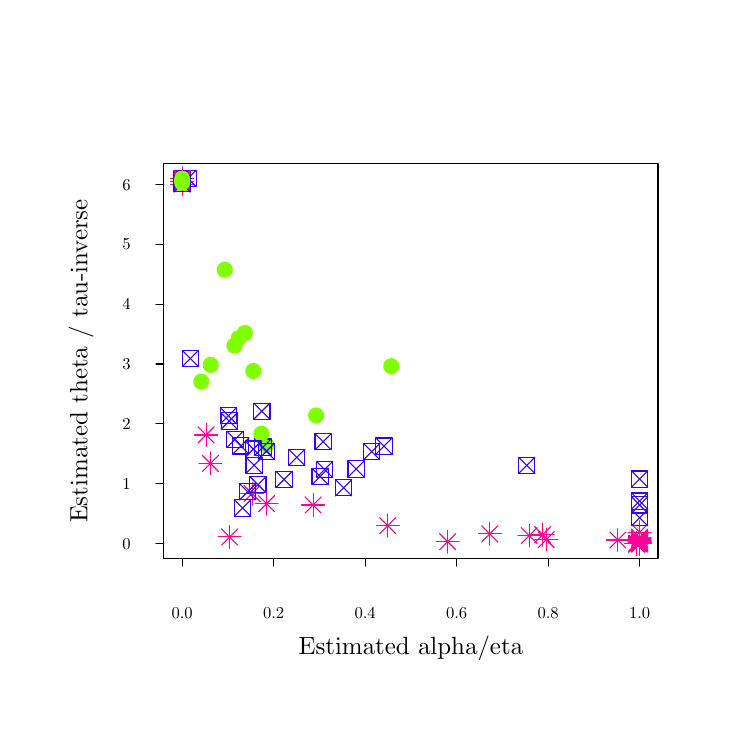
\begin{tikzpicture}[x=1pt,y=1pt]
\definecolor{fillColor}{RGB}{255,255,255}
\path[use as bounding box,fill=fillColor,fill opacity=0.00] (0,0) rectangle (252.94,252.94);
\begin{scope}
\path[clip] ( 49.20, 61.20) rectangle (227.75,203.75);
\definecolor{drawColor}{RGB}{255,0,153}

\path[draw=drawColor,line width= 0.4pt,line join=round,line cap=round] (218.21, 67.70) -- (224.06, 73.55);

\path[draw=drawColor,line width= 0.4pt,line join=round,line cap=round] (218.21, 73.55) -- (224.06, 67.70);

\path[draw=drawColor,line width= 0.4pt,line join=round,line cap=round] (216.99, 70.63) -- (225.27, 70.63);

\path[draw=drawColor,line width= 0.4pt,line join=round,line cap=round] (221.13, 66.49) -- (221.13, 74.77);

\path[draw=drawColor,line width= 0.4pt,line join=round,line cap=round] (218.21, 64.53) -- (224.06, 70.38);

\path[draw=drawColor,line width= 0.4pt,line join=round,line cap=round] (218.21, 70.38) -- (224.06, 64.53);

\path[draw=drawColor,line width= 0.4pt,line join=round,line cap=round] (217.00, 67.46) -- (225.27, 67.46);

\path[draw=drawColor,line width= 0.4pt,line join=round,line cap=round] (221.13, 63.32) -- (221.13, 71.59);

\path[draw=drawColor,line width= 0.4pt,line join=round,line cap=round] (217.14, 63.55) -- (222.99, 69.40);

\path[draw=drawColor,line width= 0.4pt,line join=round,line cap=round] (217.14, 69.40) -- (222.99, 63.55);

\path[draw=drawColor,line width= 0.4pt,line join=round,line cap=round] (215.93, 66.48) -- (224.21, 66.48);

\path[draw=drawColor,line width= 0.4pt,line join=round,line cap=round] (220.07, 62.34) -- (220.07, 70.62);
\definecolor{fillColor}{RGB}{128,255,0}

\path[fill=fillColor] ( 55.81,196.36) circle (  2.92);

\path[draw=drawColor,line width= 0.4pt,line join=round,line cap=round] ( 52.89,193.48) -- ( 58.74,199.33);

\path[draw=drawColor,line width= 0.4pt,line join=round,line cap=round] ( 52.89,199.33) -- ( 58.74,193.48);

\path[draw=drawColor,line width= 0.4pt,line join=round,line cap=round] ( 51.68,196.40) -- ( 59.95,196.40);

\path[draw=drawColor,line width= 0.4pt,line join=round,line cap=round] ( 55.81,192.27) -- ( 55.81,200.54);
\definecolor{drawColor}{RGB}{51,0,255}

\path[draw=drawColor,line width= 0.4pt,line join=round,line cap=round] (218.21, 78.96) rectangle (224.06, 84.81);

\path[draw=drawColor,line width= 0.4pt,line join=round,line cap=round] (218.21, 78.96) -- (224.06, 84.81);

\path[draw=drawColor,line width= 0.4pt,line join=round,line cap=round] (218.21, 84.81) -- (224.06, 78.96);

\path[fill=fillColor] ( 55.81,197.86) circle (  2.92);

\path[fill=fillColor] ( 55.81,197.47) circle (  2.92);

\path[fill=fillColor] ( 55.81,197.08) circle (  2.92);

\path[draw=drawColor,line width= 0.4pt,line join=round,line cap=round] ( 74.10, 98.87) rectangle ( 79.95,104.72);

\path[draw=drawColor,line width= 0.4pt,line join=round,line cap=round] ( 74.10, 98.87) -- ( 79.95,104.72);

\path[draw=drawColor,line width= 0.4pt,line join=round,line cap=round] ( 74.10,104.72) -- ( 79.95, 98.87);

\path[fill=fillColor] ( 78.50,142.61) circle (  2.92);

\path[draw=drawColor,line width= 0.4pt,line join=round,line cap=round] ( 52.89,195.14) rectangle ( 58.74,200.99);

\path[draw=drawColor,line width= 0.4pt,line join=round,line cap=round] ( 52.89,195.14) -- ( 58.74,200.99);

\path[draw=drawColor,line width= 0.4pt,line join=round,line cap=round] ( 52.89,200.99) -- ( 58.74,195.14);

\path[draw=drawColor,line width= 0.4pt,line join=round,line cap=round] (218.21, 86.91) rectangle (224.06, 92.76);

\path[draw=drawColor,line width= 0.4pt,line join=round,line cap=round] (218.21, 86.91) -- (224.06, 92.76);

\path[draw=drawColor,line width= 0.4pt,line join=round,line cap=round] (218.21, 92.76) -- (224.06, 86.91);
\definecolor{drawColor}{RGB}{255,0,153}

\path[draw=drawColor,line width= 0.4pt,line join=round,line cap=round] (184.42, 65.01) -- (190.27, 70.86);

\path[draw=drawColor,line width= 0.4pt,line join=round,line cap=round] (184.42, 70.86) -- (190.27, 65.01);

\path[draw=drawColor,line width= 0.4pt,line join=round,line cap=round] (183.21, 67.94) -- (191.49, 67.94);

\path[draw=drawColor,line width= 0.4pt,line join=round,line cap=round] (187.35, 63.80) -- (187.35, 72.07);
\definecolor{drawColor}{RGB}{51,0,255}

\path[draw=drawColor,line width= 0.4pt,line join=round,line cap=round] ( 81.70,111.44) rectangle ( 87.55,117.29);

\path[draw=drawColor,line width= 0.4pt,line join=round,line cap=round] ( 81.70,111.44) -- ( 87.55,117.29);

\path[draw=drawColor,line width= 0.4pt,line join=round,line cap=round] ( 81.70,117.29) -- ( 87.55,111.44);

\path[draw=drawColor,line width= 0.4pt,line join=round,line cap=round] (103.84,100.41) rectangle (109.69,106.26);

\path[draw=drawColor,line width= 0.4pt,line join=round,line cap=round] (103.84,100.41) -- (109.69,106.26);

\path[draw=drawColor,line width= 0.4pt,line join=round,line cap=round] (103.84,106.26) -- (109.69,100.41);

\path[draw=drawColor,line width= 0.4pt,line join=round,line cap=round] (104.36, 90.35) rectangle (110.21, 96.20);

\path[draw=drawColor,line width= 0.4pt,line join=round,line cap=round] (104.36, 90.35) -- (110.21, 96.20);

\path[draw=drawColor,line width= 0.4pt,line join=round,line cap=round] (104.36, 96.20) -- (110.21, 90.35);

\path[fill=fillColor] ( 55.81,196.52) circle (  2.92);

\path[fill=fillColor] ( 86.26,102.07) circle (  2.92);
\definecolor{drawColor}{RGB}{255,0,153}

\path[draw=drawColor,line width= 0.4pt,line join=round,line cap=round] (218.21, 64.28) -- (224.06, 70.13);

\path[draw=drawColor,line width= 0.4pt,line join=round,line cap=round] (218.21, 70.13) -- (224.06, 64.28);

\path[draw=drawColor,line width= 0.4pt,line join=round,line cap=round] (217.00, 67.20) -- (225.27, 67.20);

\path[draw=drawColor,line width= 0.4pt,line join=round,line cap=round] (221.13, 63.07) -- (221.13, 71.34);

\path[draw=drawColor,line width= 0.4pt,line join=round,line cap=round] (218.09, 63.55) -- (223.94, 69.40);

\path[draw=drawColor,line width= 0.4pt,line join=round,line cap=round] (218.09, 69.40) -- (223.94, 63.55);

\path[draw=drawColor,line width= 0.4pt,line join=round,line cap=round] (216.88, 66.48) -- (225.15, 66.48);

\path[draw=drawColor,line width= 0.4pt,line join=round,line cap=round] (221.01, 62.34) -- (221.01, 70.62);
\definecolor{drawColor}{RGB}{51,0,255}

\path[draw=drawColor,line width= 0.4pt,line join=round,line cap=round] ( 89.70, 86.76) rectangle ( 95.55, 92.61);

\path[draw=drawColor,line width= 0.4pt,line join=round,line cap=round] ( 89.70, 86.76) -- ( 95.55, 92.61);

\path[draw=drawColor,line width= 0.4pt,line join=round,line cap=round] ( 89.70, 92.61) -- ( 95.55, 86.76);
\definecolor{drawColor}{RGB}{255,0,153}

\path[draw=drawColor,line width= 0.4pt,line join=round,line cap=round] (148.84, 64.28) -- (154.69, 70.13);

\path[draw=drawColor,line width= 0.4pt,line join=round,line cap=round] (148.84, 70.13) -- (154.69, 64.28);

\path[draw=drawColor,line width= 0.4pt,line join=round,line cap=round] (147.63, 67.21) -- (155.90, 67.21);

\path[draw=drawColor,line width= 0.4pt,line join=round,line cap=round] (151.76, 63.07) -- (151.76, 71.34);

\path[draw=drawColor,line width= 0.4pt,line join=round,line cap=round] ( 52.89,194.35) -- ( 58.74,200.20);

\path[draw=drawColor,line width= 0.4pt,line join=round,line cap=round] ( 52.89,200.20) -- ( 58.74,194.35);

\path[draw=drawColor,line width= 0.4pt,line join=round,line cap=round] ( 51.68,197.28) -- ( 59.95,197.28);

\path[draw=drawColor,line width= 0.4pt,line join=round,line cap=round] ( 55.81,193.14) -- ( 55.81,201.41);

\path[draw=drawColor,line width= 0.4pt,line join=round,line cap=round] (218.09, 63.55) -- (223.94, 69.40);

\path[draw=drawColor,line width= 0.4pt,line join=round,line cap=round] (218.09, 69.40) -- (223.94, 63.55);

\path[draw=drawColor,line width= 0.4pt,line join=round,line cap=round] (216.88, 66.48) -- (225.15, 66.48);

\path[draw=drawColor,line width= 0.4pt,line join=round,line cap=round] (221.01, 62.34) -- (221.01, 70.62);

\path[fill=fillColor] (131.39,130.60) circle (  2.92);

\path[fill=fillColor] ( 62.76,125.04) circle (  2.92);

\path[draw=drawColor,line width= 0.4pt,line join=round,line cap=round] (217.14, 63.55) -- (222.99, 69.40);

\path[draw=drawColor,line width= 0.4pt,line join=round,line cap=round] (217.14, 69.40) -- (222.99, 63.55);

\path[draw=drawColor,line width= 0.4pt,line join=round,line cap=round] (215.93, 66.48) -- (224.21, 66.48);

\path[draw=drawColor,line width= 0.4pt,line join=round,line cap=round] (220.07, 62.34) -- (220.07, 70.62);

\path[draw=drawColor,line width= 0.4pt,line join=round,line cap=round] (100.20, 77.54) -- (106.05, 83.39);

\path[draw=drawColor,line width= 0.4pt,line join=round,line cap=round] (100.20, 83.39) -- (106.05, 77.54);

\path[draw=drawColor,line width= 0.4pt,line join=round,line cap=round] ( 98.99, 80.47) -- (107.27, 80.47);

\path[draw=drawColor,line width= 0.4pt,line join=round,line cap=round] (103.13, 76.33) -- (103.13, 84.60);
\definecolor{drawColor}{RGB}{51,0,255}

\path[draw=drawColor,line width= 0.4pt,line join=round,line cap=round] ( 83.30, 96.87) rectangle ( 89.15,102.72);

\path[draw=drawColor,line width= 0.4pt,line join=round,line cap=round] ( 83.30, 96.87) -- ( 89.15,102.72);

\path[draw=drawColor,line width= 0.4pt,line join=round,line cap=round] ( 83.30,102.72) -- ( 89.15, 96.87);
\definecolor{drawColor}{RGB}{255,0,153}

\path[draw=drawColor,line width= 0.4pt,line join=round,line cap=round] (218.09, 63.55) -- (223.94, 69.40);

\path[draw=drawColor,line width= 0.4pt,line join=round,line cap=round] (218.09, 69.40) -- (223.94, 63.55);

\path[draw=drawColor,line width= 0.4pt,line join=round,line cap=round] (216.88, 66.48) -- (225.15, 66.48);

\path[draw=drawColor,line width= 0.4pt,line join=round,line cap=round] (221.01, 62.34) -- (221.01, 70.62);
\definecolor{drawColor}{RGB}{51,0,255}

\path[draw=drawColor,line width= 0.4pt,line join=round,line cap=round] ( 94.31, 94.76) rectangle (100.16,100.61);

\path[draw=drawColor,line width= 0.4pt,line join=round,line cap=round] ( 94.31, 94.76) -- (100.16,100.61);

\path[draw=drawColor,line width= 0.4pt,line join=round,line cap=round] ( 94.31,100.61) -- (100.16, 94.76);

\path[draw=drawColor,line width= 0.4pt,line join=round,line cap=round] ( 69.59,109.77) rectangle ( 75.44,115.62);

\path[draw=drawColor,line width= 0.4pt,line join=round,line cap=round] ( 69.59,109.77) -- ( 75.44,115.62);

\path[draw=drawColor,line width= 0.4pt,line join=round,line cap=round] ( 69.59,115.62) -- ( 75.44,109.77);
\definecolor{drawColor}{RGB}{255,0,153}

\path[draw=drawColor,line width= 0.4pt,line join=round,line cap=round] ( 52.89,194.28) -- ( 58.74,200.13);

\path[draw=drawColor,line width= 0.4pt,line join=round,line cap=round] ( 52.89,200.13) -- ( 58.74,194.28);

\path[draw=drawColor,line width= 0.4pt,line join=round,line cap=round] ( 51.68,197.20) -- ( 59.95,197.20);

\path[draw=drawColor,line width= 0.4pt,line join=round,line cap=round] ( 55.81,193.07) -- ( 55.81,201.34);

\path[draw=drawColor,line width= 0.4pt,line join=round,line cap=round] (218.21, 63.55) -- (224.06, 69.40);

\path[draw=drawColor,line width= 0.4pt,line join=round,line cap=round] (218.21, 69.40) -- (224.06, 63.55);

\path[draw=drawColor,line width= 0.4pt,line join=round,line cap=round] (217.00, 66.48) -- (225.27, 66.48);

\path[draw=drawColor,line width= 0.4pt,line join=round,line cap=round] (221.13, 62.34) -- (221.13, 70.62);
\definecolor{drawColor}{RGB}{51,0,255}

\path[draw=drawColor,line width= 0.4pt,line join=round,line cap=round] ( 55.00,195.52) rectangle ( 60.85,201.37);

\path[draw=drawColor,line width= 0.4pt,line join=round,line cap=round] ( 55.00,195.52) -- ( 60.85,201.37);

\path[draw=drawColor,line width= 0.4pt,line join=round,line cap=round] ( 55.00,201.37) -- ( 60.85,195.52);

\path[draw=drawColor,line width= 0.4pt,line join=round,line cap=round] ( 82.10, 98.45) rectangle ( 87.95,104.30);

\path[draw=drawColor,line width= 0.4pt,line join=round,line cap=round] ( 82.10, 98.45) -- ( 87.95,104.30);

\path[draw=drawColor,line width= 0.4pt,line join=round,line cap=round] ( 82.10,104.30) -- ( 87.95, 98.45);

\path[fill=fillColor] ( 55.81,197.24) circle (  2.92);
\definecolor{drawColor}{RGB}{255,0,153}

\path[draw=drawColor,line width= 0.4pt,line join=round,line cap=round] ( 63.12, 92.55) -- ( 68.97, 98.40);

\path[draw=drawColor,line width= 0.4pt,line join=round,line cap=round] ( 63.12, 98.40) -- ( 68.97, 92.55);

\path[draw=drawColor,line width= 0.4pt,line join=round,line cap=round] ( 61.91, 95.47) -- ( 70.18, 95.47);

\path[draw=drawColor,line width= 0.4pt,line join=round,line cap=round] ( 66.04, 91.34) -- ( 66.04, 99.61);
\definecolor{drawColor}{RGB}{51,0,255}

\path[draw=drawColor,line width= 0.4pt,line join=round,line cap=round] (102.75, 87.84) rectangle (108.60, 93.69);

\path[draw=drawColor,line width= 0.4pt,line join=round,line cap=round] (102.75, 87.84) -- (108.60, 93.69);

\path[draw=drawColor,line width= 0.4pt,line join=round,line cap=round] (102.75, 93.69) -- (108.60, 87.84);

\path[fill=fillColor] ( 55.81,196.40) circle (  2.92);
\definecolor{drawColor}{RGB}{255,0,153}

\path[draw=drawColor,line width= 0.4pt,line join=round,line cap=round] (217.14, 63.55) -- (222.99, 69.40);

\path[draw=drawColor,line width= 0.4pt,line join=round,line cap=round] (217.14, 69.40) -- (222.99, 63.55);

\path[draw=drawColor,line width= 0.4pt,line join=round,line cap=round] (215.93, 66.48) -- (224.21, 66.48);

\path[draw=drawColor,line width= 0.4pt,line join=round,line cap=round] (220.07, 62.34) -- (220.07, 70.62);

\path[fill=fillColor] ( 76.29,140.79) circle (  2.92);

\path[draw=drawColor,line width= 0.4pt,line join=round,line cap=round] ( 61.54,102.85) -- ( 67.39,108.70);

\path[draw=drawColor,line width= 0.4pt,line join=round,line cap=round] ( 61.54,108.70) -- ( 67.39,102.85);

\path[draw=drawColor,line width= 0.4pt,line join=round,line cap=round] ( 60.33,105.77) -- ( 68.60,105.77);

\path[draw=drawColor,line width= 0.4pt,line join=round,line cap=round] ( 64.47,101.64) -- ( 64.47,109.91);

\path[draw=drawColor,line width= 0.4pt,line join=round,line cap=round] (217.14, 63.55) -- (222.99, 69.40);

\path[draw=drawColor,line width= 0.4pt,line join=round,line cap=round] (217.14, 69.40) -- (222.99, 63.55);

\path[draw=drawColor,line width= 0.4pt,line join=round,line cap=round] (215.93, 66.48) -- (224.21, 66.48);

\path[draw=drawColor,line width= 0.4pt,line join=round,line cap=round] (220.07, 62.34) -- (220.07, 70.62);
\definecolor{drawColor}{RGB}{51,0,255}

\path[draw=drawColor,line width= 0.4pt,line join=round,line cap=round] (111.26, 83.75) rectangle (117.11, 89.60);

\path[draw=drawColor,line width= 0.4pt,line join=round,line cap=round] (111.26, 83.75) -- (117.11, 89.60);

\path[draw=drawColor,line width= 0.4pt,line join=round,line cap=round] (111.26, 89.60) -- (117.11, 83.75);

\path[draw=drawColor,line width= 0.4pt,line join=round,line cap=round] ( 74.74, 76.46) rectangle ( 80.59, 82.31);

\path[draw=drawColor,line width= 0.4pt,line join=round,line cap=round] ( 74.74, 76.46) -- ( 80.59, 82.31);

\path[draw=drawColor,line width= 0.4pt,line join=round,line cap=round] ( 74.74, 82.31) -- ( 80.59, 76.46);

\path[fill=fillColor] ( 55.81,198.24) circle (  2.92);
\definecolor{drawColor}{RGB}{255,0,153}

\path[draw=drawColor,line width= 0.4pt,line join=round,line cap=round] (217.14, 63.55) -- (222.99, 69.40);

\path[draw=drawColor,line width= 0.4pt,line join=round,line cap=round] (217.14, 69.40) -- (222.99, 63.55);

\path[draw=drawColor,line width= 0.4pt,line join=round,line cap=round] (215.93, 66.48) -- (224.21, 66.48);

\path[draw=drawColor,line width= 0.4pt,line join=round,line cap=round] (220.07, 62.34) -- (220.07, 70.62);

\path[fill=fillColor] ( 55.81,197.55) circle (  2.92);

\path[fill=fillColor] ( 66.14,131.07) circle (  2.92);

\path[draw=drawColor,line width= 0.4pt,line join=round,line cap=round] ( 78.17, 81.66) -- ( 84.02, 87.51);

\path[draw=drawColor,line width= 0.4pt,line join=round,line cap=round] ( 78.17, 87.51) -- ( 84.02, 81.66);

\path[draw=drawColor,line width= 0.4pt,line join=round,line cap=round] ( 76.96, 84.59) -- ( 85.23, 84.59);

\path[draw=drawColor,line width= 0.4pt,line join=round,line cap=round] ( 81.10, 80.45) -- ( 81.10, 88.72);
\definecolor{drawColor}{RGB}{51,0,255}

\path[draw=drawColor,line width= 0.4pt,line join=round,line cap=round] ( 52.89,195.54) rectangle ( 58.74,201.39);

\path[draw=drawColor,line width= 0.4pt,line join=round,line cap=round] ( 52.89,195.54) -- ( 58.74,201.39);

\path[draw=drawColor,line width= 0.4pt,line join=round,line cap=round] ( 52.89,201.39) -- ( 58.74,195.54);
\definecolor{drawColor}{RGB}{255,0,153}

\path[draw=drawColor,line width= 0.4pt,line join=round,line cap=round] (178.32, 66.48) -- (184.17, 72.33);

\path[draw=drawColor,line width= 0.4pt,line join=round,line cap=round] (178.32, 72.33) -- (184.17, 66.48);

\path[draw=drawColor,line width= 0.4pt,line join=round,line cap=round] (177.11, 69.41) -- (185.38, 69.41);

\path[draw=drawColor,line width= 0.4pt,line join=round,line cap=round] (181.25, 65.27) -- (181.25, 73.54);

\path[fill=fillColor] ( 81.52,128.87) circle (  2.92);

\path[fill=fillColor] ( 71.21,165.47) circle (  2.92);

\path[draw=drawColor,line width= 0.4pt,line join=round,line cap=round] ( 52.89,194.34) -- ( 58.74,200.19);

\path[draw=drawColor,line width= 0.4pt,line join=round,line cap=round] ( 52.89,200.19) -- ( 58.74,194.34);

\path[draw=drawColor,line width= 0.4pt,line join=round,line cap=round] ( 51.68,197.27) -- ( 59.95,197.27);

\path[draw=drawColor,line width= 0.4pt,line join=round,line cap=round] ( 55.81,193.13) -- ( 55.81,201.40);

\path[draw=drawColor,line width= 0.4pt,line join=round,line cap=round] ( 52.89,195.48) -- ( 58.74,201.33);

\path[draw=drawColor,line width= 0.4pt,line join=round,line cap=round] ( 52.89,201.33) -- ( 58.74,195.48);

\path[draw=drawColor,line width= 0.4pt,line join=round,line cap=round] ( 51.68,198.41) -- ( 59.95,198.41);

\path[draw=drawColor,line width= 0.4pt,line join=round,line cap=round] ( 55.81,194.27) -- ( 55.81,202.55);
\definecolor{drawColor}{RGB}{51,0,255}

\path[draw=drawColor,line width= 0.4pt,line join=round,line cap=round] (218.21, 77.56) rectangle (224.06, 83.41);

\path[draw=drawColor,line width= 0.4pt,line join=round,line cap=round] (218.21, 77.56) -- (224.06, 83.41);

\path[draw=drawColor,line width= 0.4pt,line join=round,line cap=round] (218.21, 83.41) -- (224.06, 77.56);

\path[draw=drawColor,line width= 0.4pt,line join=round,line cap=round] ( 76.56, 82.29) rectangle ( 82.41, 88.14);

\path[draw=drawColor,line width= 0.4pt,line join=round,line cap=round] ( 76.56, 82.29) -- ( 82.41, 88.14);

\path[draw=drawColor,line width= 0.4pt,line join=round,line cap=round] ( 76.56, 88.14) -- ( 82.41, 82.29);
\definecolor{drawColor}{RGB}{255,0,153}

\path[draw=drawColor,line width= 0.4pt,line join=round,line cap=round] (218.21, 64.13) -- (224.06, 69.98);

\path[draw=drawColor,line width= 0.4pt,line join=round,line cap=round] (218.21, 69.98) -- (224.06, 64.13);

\path[draw=drawColor,line width= 0.4pt,line join=round,line cap=round] (217.00, 67.06) -- (225.27, 67.06);

\path[draw=drawColor,line width= 0.4pt,line join=round,line cap=round] (221.13, 62.92) -- (221.13, 71.19);
\definecolor{drawColor}{RGB}{51,0,255}

\path[draw=drawColor,line width= 0.4pt,line join=round,line cap=round] ( 71.99,101.26) rectangle ( 77.84,107.11);

\path[draw=drawColor,line width= 0.4pt,line join=round,line cap=round] ( 71.99,101.26) -- ( 77.84,107.11);

\path[draw=drawColor,line width= 0.4pt,line join=round,line cap=round] ( 71.99,107.11) -- ( 77.84,101.26);
\definecolor{drawColor}{RGB}{255,0,153}

\path[draw=drawColor,line width= 0.4pt,line join=round,line cap=round] (218.21, 63.55) -- (224.06, 69.40);

\path[draw=drawColor,line width= 0.4pt,line join=round,line cap=round] (218.21, 69.40) -- (224.06, 63.55);

\path[draw=drawColor,line width= 0.4pt,line join=round,line cap=round] (217.00, 66.48) -- (225.27, 66.48);

\path[draw=drawColor,line width= 0.4pt,line join=round,line cap=round] (221.13, 62.34) -- (221.13, 70.62);

\path[draw=drawColor,line width= 0.4pt,line join=round,line cap=round] ( 70.05, 65.99) -- ( 75.90, 71.84);

\path[draw=drawColor,line width= 0.4pt,line join=round,line cap=round] ( 70.05, 71.84) -- ( 75.90, 65.99);

\path[draw=drawColor,line width= 0.4pt,line join=round,line cap=round] ( 68.84, 68.92) -- ( 77.11, 68.92);

\path[draw=drawColor,line width= 0.4pt,line join=round,line cap=round] ( 72.98, 64.78) -- ( 72.98, 73.05);
\definecolor{drawColor}{RGB}{51,0,255}

\path[draw=drawColor,line width= 0.4pt,line join=round,line cap=round] ( 55.87,130.47) rectangle ( 61.72,136.32);

\path[draw=drawColor,line width= 0.4pt,line join=round,line cap=round] ( 55.87,130.47) -- ( 61.72,136.32);

\path[draw=drawColor,line width= 0.4pt,line join=round,line cap=round] ( 55.87,136.32) -- ( 61.72,130.47);
\definecolor{drawColor}{RGB}{255,0,153}

\path[draw=drawColor,line width= 0.4pt,line join=round,line cap=round] (218.21, 65.12) -- (224.06, 70.97);

\path[draw=drawColor,line width= 0.4pt,line join=round,line cap=round] (218.21, 70.97) -- (224.06, 65.12);

\path[draw=drawColor,line width= 0.4pt,line join=round,line cap=round] (217.00, 68.05) -- (225.27, 68.05);

\path[draw=drawColor,line width= 0.4pt,line join=round,line cap=round] (221.13, 63.91) -- (221.13, 72.18);

\path[draw=drawColor,line width= 0.4pt,line join=round,line cap=round] ( 52.89,195.42) -- ( 58.74,201.27);

\path[draw=drawColor,line width= 0.4pt,line join=round,line cap=round] ( 52.89,201.27) -- ( 58.74,195.42);

\path[draw=drawColor,line width= 0.4pt,line join=round,line cap=round] ( 51.68,198.35) -- ( 59.95,198.35);

\path[draw=drawColor,line width= 0.4pt,line join=round,line cap=round] ( 55.81,194.21) -- ( 55.81,202.48);

\path[fill=fillColor] ( 84.46,106.19) circle (  2.92);
\definecolor{drawColor}{RGB}{51,0,255}

\path[draw=drawColor,line width= 0.4pt,line join=round,line cap=round] ( 80.27, 84.89) rectangle ( 86.12, 90.74);

\path[draw=drawColor,line width= 0.4pt,line join=round,line cap=round] ( 80.27, 84.89) -- ( 86.12, 90.74);

\path[draw=drawColor,line width= 0.4pt,line join=round,line cap=round] ( 80.27, 90.74) -- ( 86.12, 84.89);
\definecolor{drawColor}{RGB}{255,0,153}

\path[draw=drawColor,line width= 0.4pt,line join=round,line cap=round] (127.20, 70.09) -- (133.05, 75.94);

\path[draw=drawColor,line width= 0.4pt,line join=round,line cap=round] (127.20, 75.94) -- (133.05, 70.09);

\path[draw=drawColor,line width= 0.4pt,line join=round,line cap=round] (125.99, 73.01) -- (134.26, 73.01);

\path[draw=drawColor,line width= 0.4pt,line join=round,line cap=round] (130.13, 68.88) -- (130.13, 77.15);

\path[draw=drawColor,line width= 0.4pt,line join=round,line cap=round] ( 83.40, 78.00) -- ( 89.25, 83.85);

\path[draw=drawColor,line width= 0.4pt,line join=round,line cap=round] ( 83.40, 83.85) -- ( 89.25, 78.00);

\path[draw=drawColor,line width= 0.4pt,line join=round,line cap=round] ( 82.18, 80.93) -- ( 90.46, 80.93);

\path[draw=drawColor,line width= 0.4pt,line join=round,line cap=round] ( 86.32, 76.79) -- ( 86.32, 85.06);

\path[draw=drawColor,line width= 0.4pt,line join=round,line cap=round] (217.14, 63.55) -- (222.99, 69.40);

\path[draw=drawColor,line width= 0.4pt,line join=round,line cap=round] (217.14, 69.40) -- (222.99, 63.55);

\path[draw=drawColor,line width= 0.4pt,line join=round,line cap=round] (215.93, 66.48) -- (224.21, 66.48);

\path[draw=drawColor,line width= 0.4pt,line join=round,line cap=round] (220.07, 62.34) -- (220.07, 70.62);

\path[draw=drawColor,line width= 0.4pt,line join=round,line cap=round] ( 52.89,195.45) -- ( 58.74,201.30);

\path[draw=drawColor,line width= 0.4pt,line join=round,line cap=round] ( 52.89,201.30) -- ( 58.74,195.45);

\path[draw=drawColor,line width= 0.4pt,line join=round,line cap=round] ( 51.68,198.37) -- ( 59.95,198.37);

\path[draw=drawColor,line width= 0.4pt,line join=round,line cap=round] ( 55.81,194.23) -- ( 55.81,202.51);

\path[draw=drawColor,line width= 0.4pt,line join=round,line cap=round] ( 52.89,194.59) -- ( 58.74,200.44);

\path[draw=drawColor,line width= 0.4pt,line join=round,line cap=round] ( 52.89,200.44) -- ( 58.74,194.59);

\path[draw=drawColor,line width= 0.4pt,line join=round,line cap=round] ( 51.68,197.51) -- ( 59.95,197.51);

\path[draw=drawColor,line width= 0.4pt,line join=round,line cap=round] ( 55.81,193.38) -- ( 55.81,201.65);
\definecolor{drawColor}{RGB}{51,0,255}

\path[draw=drawColor,line width= 0.4pt,line join=round,line cap=round] ( 78.91, 91.91) rectangle ( 84.76, 97.76);

\path[draw=drawColor,line width= 0.4pt,line join=round,line cap=round] ( 78.91, 91.91) -- ( 84.76, 97.76);

\path[draw=drawColor,line width= 0.4pt,line join=round,line cap=round] ( 78.91, 97.76) -- ( 84.76, 91.91);

\path[fill=fillColor] ( 55.81,198.37) circle (  2.92);

\path[draw=drawColor,line width= 0.4pt,line join=round,line cap=round] ( 52.89,193.73) rectangle ( 58.74,199.58);

\path[draw=drawColor,line width= 0.4pt,line join=round,line cap=round] ( 52.89,193.73) -- ( 58.74,199.58);

\path[draw=drawColor,line width= 0.4pt,line join=round,line cap=round] ( 52.89,199.58) -- ( 58.74,193.73);
\definecolor{drawColor}{RGB}{255,0,153}

\path[draw=drawColor,line width= 0.4pt,line join=round,line cap=round] (217.14, 63.55) -- (222.99, 69.40);

\path[draw=drawColor,line width= 0.4pt,line join=round,line cap=round] (217.14, 69.40) -- (222.99, 63.55);

\path[draw=drawColor,line width= 0.4pt,line join=round,line cap=round] (215.93, 66.48) -- (224.21, 66.48);

\path[draw=drawColor,line width= 0.4pt,line join=round,line cap=round] (220.07, 62.34) -- (220.07, 70.62);

\path[draw=drawColor,line width= 0.4pt,line join=round,line cap=round] (217.14, 63.55) -- (222.99, 69.40);

\path[draw=drawColor,line width= 0.4pt,line join=round,line cap=round] (217.14, 69.40) -- (222.99, 63.55);

\path[draw=drawColor,line width= 0.4pt,line join=round,line cap=round] (215.93, 66.48) -- (224.21, 66.48);

\path[draw=drawColor,line width= 0.4pt,line join=round,line cap=round] (220.07, 62.34) -- (220.07, 70.62);
\definecolor{drawColor}{RGB}{51,0,255}

\path[draw=drawColor,line width= 0.4pt,line join=round,line cap=round] (115.76, 90.55) rectangle (121.61, 96.40);

\path[draw=drawColor,line width= 0.4pt,line join=round,line cap=round] (115.76, 90.55) -- (121.61, 96.40);

\path[draw=drawColor,line width= 0.4pt,line join=round,line cap=round] (115.76, 96.40) -- (121.61, 90.55);

\path[fill=fillColor] ( 74.73,138.05) circle (  2.92);
\definecolor{drawColor}{RGB}{255,0,153}

\path[draw=drawColor,line width= 0.4pt,line join=round,line cap=round] (217.14, 63.55) -- (222.99, 69.40);

\path[draw=drawColor,line width= 0.4pt,line join=round,line cap=round] (217.14, 69.40) -- (222.99, 63.55);

\path[draw=drawColor,line width= 0.4pt,line join=round,line cap=round] (215.93, 66.48) -- (224.21, 66.48);

\path[draw=drawColor,line width= 0.4pt,line join=round,line cap=round] (220.07, 62.34) -- (220.07, 70.62);

\path[fill=fillColor] (104.23,112.82) circle (  2.92);

\path[draw=drawColor,line width= 0.4pt,line join=round,line cap=round] (218.21, 63.55) -- (224.06, 69.40);

\path[draw=drawColor,line width= 0.4pt,line join=round,line cap=round] (218.21, 69.40) -- (224.06, 63.55);

\path[draw=drawColor,line width= 0.4pt,line join=round,line cap=round] (217.00, 66.48) -- (225.27, 66.48);

\path[draw=drawColor,line width= 0.4pt,line join=round,line cap=round] (221.13, 62.34) -- (221.13, 70.62);

\path[draw=drawColor,line width= 0.4pt,line join=round,line cap=round] (217.14, 63.55) -- (222.99, 69.40);

\path[draw=drawColor,line width= 0.4pt,line join=round,line cap=round] (217.14, 69.40) -- (222.99, 63.55);

\path[draw=drawColor,line width= 0.4pt,line join=round,line cap=round] (215.93, 66.48) -- (224.21, 66.48);

\path[draw=drawColor,line width= 0.4pt,line join=round,line cap=round] (220.07, 62.34) -- (220.07, 70.62);
\definecolor{drawColor}{RGB}{51,0,255}

\path[draw=drawColor,line width= 0.4pt,line join=round,line cap=round] (121.40, 96.82) rectangle (127.25,102.67);

\path[draw=drawColor,line width= 0.4pt,line join=round,line cap=round] (121.40, 96.82) -- (127.25,102.67);

\path[draw=drawColor,line width= 0.4pt,line join=round,line cap=round] (121.40,102.67) -- (127.25, 96.82);
\definecolor{drawColor}{RGB}{255,0,153}

\path[draw=drawColor,line width= 0.4pt,line join=round,line cap=round] (218.21, 63.55) -- (224.06, 69.40);

\path[draw=drawColor,line width= 0.4pt,line join=round,line cap=round] (218.21, 69.40) -- (224.06, 63.55);

\path[draw=drawColor,line width= 0.4pt,line join=round,line cap=round] (217.00, 66.48) -- (225.27, 66.48);

\path[draw=drawColor,line width= 0.4pt,line join=round,line cap=round] (221.13, 62.34) -- (221.13, 70.62);

\path[fill=fillColor] ( 55.81,198.10) circle (  2.92);
\definecolor{drawColor}{RGB}{51,0,255}

\path[draw=drawColor,line width= 0.4pt,line join=round,line cap=round] ( 69.90,107.88) rectangle ( 75.75,113.73);

\path[draw=drawColor,line width= 0.4pt,line join=round,line cap=round] ( 69.90,107.88) -- ( 75.75,113.73);

\path[draw=drawColor,line width= 0.4pt,line join=round,line cap=round] ( 69.90,113.73) -- ( 75.75,107.88);
\definecolor{drawColor}{RGB}{255,0,153}

\path[draw=drawColor,line width= 0.4pt,line join=round,line cap=round] (217.14, 63.55) -- (222.99, 69.40);

\path[draw=drawColor,line width= 0.4pt,line join=round,line cap=round] (217.14, 69.40) -- (222.99, 63.55);

\path[draw=drawColor,line width= 0.4pt,line join=round,line cap=round] (215.93, 66.48) -- (224.21, 66.48);

\path[draw=drawColor,line width= 0.4pt,line join=round,line cap=round] (220.07, 62.34) -- (220.07, 70.62);

\path[draw=drawColor,line width= 0.4pt,line join=round,line cap=round] (164.06, 67.09) -- (169.91, 72.94);

\path[draw=drawColor,line width= 0.4pt,line join=round,line cap=round] (164.06, 72.94) -- (169.91, 67.09);

\path[draw=drawColor,line width= 0.4pt,line join=round,line cap=round] (162.85, 70.02) -- (171.12, 70.02);

\path[draw=drawColor,line width= 0.4pt,line join=round,line cap=round] (166.99, 65.88) -- (166.99, 74.15);
\definecolor{drawColor}{RGB}{51,0,255}

\path[draw=drawColor,line width= 0.4pt,line join=round,line cap=round] (125.84, 98.82) rectangle (131.69,104.67);

\path[draw=drawColor,line width= 0.4pt,line join=round,line cap=round] (125.84, 98.82) -- (131.69,104.67);

\path[draw=drawColor,line width= 0.4pt,line join=round,line cap=round] (125.84,104.67) -- (131.69, 98.82);

\path[draw=drawColor,line width= 0.4pt,line join=round,line cap=round] ( 78.63, 97.72) rectangle ( 84.48,103.57);

\path[draw=drawColor,line width= 0.4pt,line join=round,line cap=round] ( 78.63, 97.72) -- ( 84.48,103.57);

\path[draw=drawColor,line width= 0.4pt,line join=round,line cap=round] ( 78.63,103.57) -- ( 84.48, 97.72);
\definecolor{drawColor}{RGB}{255,0,153}

\path[draw=drawColor,line width= 0.4pt,line join=round,line cap=round] (218.21, 65.39) -- (224.06, 71.24);

\path[draw=drawColor,line width= 0.4pt,line join=round,line cap=round] (218.21, 71.24) -- (224.06, 65.39);

\path[draw=drawColor,line width= 0.4pt,line join=round,line cap=round] (217.00, 68.32) -- (225.27, 68.32);

\path[draw=drawColor,line width= 0.4pt,line join=round,line cap=round] (221.13, 64.18) -- (221.13, 72.46);

\path[draw=drawColor,line width= 0.4pt,line join=round,line cap=round] (217.14, 63.55) -- (222.99, 69.40);

\path[draw=drawColor,line width= 0.4pt,line join=round,line cap=round] (217.14, 69.40) -- (222.99, 63.55);

\path[draw=drawColor,line width= 0.4pt,line join=round,line cap=round] (215.93, 66.48) -- (224.21, 66.48);

\path[draw=drawColor,line width= 0.4pt,line join=round,line cap=round] (220.07, 62.34) -- (220.07, 70.62);
\definecolor{drawColor}{RGB}{51,0,255}

\path[draw=drawColor,line width= 0.4pt,line join=round,line cap=round] (218.21, 72.94) rectangle (224.06, 78.79);

\path[draw=drawColor,line width= 0.4pt,line join=round,line cap=round] (218.21, 72.94) -- (224.06, 78.79);

\path[draw=drawColor,line width= 0.4pt,line join=round,line cap=round] (218.21, 78.79) -- (224.06, 72.94);
\definecolor{drawColor}{RGB}{255,0,153}

\path[draw=drawColor,line width= 0.4pt,line join=round,line cap=round] (210.35, 64.88) -- (216.20, 70.73);

\path[draw=drawColor,line width= 0.4pt,line join=round,line cap=round] (210.35, 70.73) -- (216.20, 64.88);

\path[draw=drawColor,line width= 0.4pt,line join=round,line cap=round] (209.14, 67.81) -- (217.41, 67.81);

\path[draw=drawColor,line width= 0.4pt,line join=round,line cap=round] (213.27, 63.67) -- (213.27, 71.94);

\path[fill=fillColor] ( 55.81,197.65) circle (  2.92);

\path[draw=drawColor,line width= 0.4pt,line join=round,line cap=round] (218.20, 63.89) -- (224.05, 69.74);

\path[draw=drawColor,line width= 0.4pt,line join=round,line cap=round] (218.20, 69.74) -- (224.05, 63.89);

\path[draw=drawColor,line width= 0.4pt,line join=round,line cap=round] (216.99, 66.82) -- (225.26, 66.82);

\path[draw=drawColor,line width= 0.4pt,line join=round,line cap=round] (221.13, 62.68) -- (221.13, 70.95);

\path[draw=drawColor,line width= 0.4pt,line join=round,line cap=round] (217.14, 63.55) -- (222.99, 69.40);

\path[draw=drawColor,line width= 0.4pt,line join=round,line cap=round] (217.14, 69.40) -- (222.99, 63.55);

\path[draw=drawColor,line width= 0.4pt,line join=round,line cap=round] (215.93, 66.48) -- (224.21, 66.48);

\path[draw=drawColor,line width= 0.4pt,line join=round,line cap=round] (220.07, 62.34) -- (220.07, 70.62);

\path[draw=drawColor,line width= 0.4pt,line join=round,line cap=round] (218.21, 65.90) -- (224.06, 71.75);

\path[draw=drawColor,line width= 0.4pt,line join=round,line cap=round] (218.21, 71.75) -- (224.06, 65.90);

\path[draw=drawColor,line width= 0.4pt,line join=round,line cap=round] (217.00, 68.83) -- (225.27, 68.83);

\path[draw=drawColor,line width= 0.4pt,line join=round,line cap=round] (221.13, 64.69) -- (221.13, 72.97);

\path[draw=drawColor,line width= 0.4pt,line join=round,line cap=round] (183.17, 66.80) -- (189.02, 72.65);

\path[draw=drawColor,line width= 0.4pt,line join=round,line cap=round] (183.17, 72.65) -- (189.02, 66.80);

\path[draw=drawColor,line width= 0.4pt,line join=round,line cap=round] (181.96, 69.72) -- (190.23, 69.72);

\path[draw=drawColor,line width= 0.4pt,line join=round,line cap=round] (186.10, 65.59) -- (186.10, 73.86);

\path[fill=fillColor] ( 55.81,197.02) circle (  2.92);
\definecolor{drawColor}{RGB}{51,0,255}

\path[draw=drawColor,line width= 0.4pt,line join=round,line cap=round] (177.43, 91.84) rectangle (183.28, 97.69);

\path[draw=drawColor,line width= 0.4pt,line join=round,line cap=round] (177.43, 91.84) -- (183.28, 97.69);

\path[draw=drawColor,line width= 0.4pt,line join=round,line cap=round] (177.43, 97.69) -- (183.28, 91.84);
\end{scope}
\begin{scope}
\path[clip] (  0.00,  0.00) rectangle (252.94,252.94);
\definecolor{drawColor}{RGB}{0,0,0}

\path[draw=drawColor,line width= 0.4pt,line join=round,line cap=round] ( 55.81, 61.20) -- (221.13, 61.20);

\path[draw=drawColor,line width= 0.4pt,line join=round,line cap=round] ( 55.81, 61.20) -- ( 55.81, 58.35);

\path[draw=drawColor,line width= 0.4pt,line join=round,line cap=round] ( 88.88, 61.20) -- ( 88.88, 58.35);

\path[draw=drawColor,line width= 0.4pt,line join=round,line cap=round] (121.94, 61.20) -- (121.94, 58.35);

\path[draw=drawColor,line width= 0.4pt,line join=round,line cap=round] (155.00, 61.20) -- (155.00, 58.35);

\path[draw=drawColor,line width= 0.4pt,line join=round,line cap=round] (188.07, 61.20) -- (188.07, 58.35);

\path[draw=drawColor,line width= 0.4pt,line join=round,line cap=round] (221.13, 61.20) -- (221.13, 58.35);

\node[text=drawColor,anchor=base,inner sep=0pt, outer sep=0pt, scale=  0.60] at ( 55.81, 39.60) {0.0};

\node[text=drawColor,anchor=base,inner sep=0pt, outer sep=0pt, scale=  0.60] at ( 88.88, 39.60) {0.2};

\node[text=drawColor,anchor=base,inner sep=0pt, outer sep=0pt, scale=  0.60] at (121.94, 39.60) {0.4};

\node[text=drawColor,anchor=base,inner sep=0pt, outer sep=0pt, scale=  0.60] at (155.00, 39.60) {0.6};

\node[text=drawColor,anchor=base,inner sep=0pt, outer sep=0pt, scale=  0.60] at (188.07, 39.60) {0.8};

\node[text=drawColor,anchor=base,inner sep=0pt, outer sep=0pt, scale=  0.60] at (221.13, 39.60) {1.0};

\path[draw=drawColor,line width= 0.4pt,line join=round,line cap=round] ( 49.20, 66.48) -- ( 49.20,196.32);

\path[draw=drawColor,line width= 0.4pt,line join=round,line cap=round] ( 49.20, 66.48) -- ( 46.35, 66.48);

\path[draw=drawColor,line width= 0.4pt,line join=round,line cap=round] ( 49.20, 88.12) -- ( 46.35, 88.12);

\path[draw=drawColor,line width= 0.4pt,line join=round,line cap=round] ( 49.20,109.76) -- ( 46.35,109.76);

\path[draw=drawColor,line width= 0.4pt,line join=round,line cap=round] ( 49.20,131.40) -- ( 46.35,131.40);

\path[draw=drawColor,line width= 0.4pt,line join=round,line cap=round] ( 49.20,153.04) -- ( 46.35,153.04);

\path[draw=drawColor,line width= 0.4pt,line join=round,line cap=round] ( 49.20,174.68) -- ( 46.35,174.68);

\path[draw=drawColor,line width= 0.4pt,line join=round,line cap=round] ( 49.20,196.32) -- ( 46.35,196.32);

\node[text=drawColor,anchor=base east,inner sep=0pt, outer sep=0pt, scale=  0.60] at ( 37.20, 64.41) {0};

\node[text=drawColor,anchor=base east,inner sep=0pt, outer sep=0pt, scale=  0.60] at ( 37.20, 86.05) {1};

\node[text=drawColor,anchor=base east,inner sep=0pt, outer sep=0pt, scale=  0.60] at ( 37.20,107.69) {2};

\node[text=drawColor,anchor=base east,inner sep=0pt, outer sep=0pt, scale=  0.60] at ( 37.20,129.33) {3};

\node[text=drawColor,anchor=base east,inner sep=0pt, outer sep=0pt, scale=  0.60] at ( 37.20,150.97) {4};

\node[text=drawColor,anchor=base east,inner sep=0pt, outer sep=0pt, scale=  0.60] at ( 37.20,172.61) {5};

\node[text=drawColor,anchor=base east,inner sep=0pt, outer sep=0pt, scale=  0.60] at ( 37.20,194.25) {6};

\path[draw=drawColor,line width= 0.4pt,line join=round,line cap=round] ( 49.20, 61.20) --
	(227.75, 61.20) --
	(227.75,203.75) --
	( 49.20,203.75) --
	( 49.20, 61.20);
\end{scope}
\begin{scope}
\path[clip] (  0.00,  0.00) rectangle (252.94,252.94);
\definecolor{drawColor}{RGB}{0,0,0}

\node[text=drawColor,anchor=base,inner sep=0pt, outer sep=0pt, scale=  0.90] at (138.47, 26.40) {Estimated alpha/eta};

\node[text=drawColor,rotate= 90.00,anchor=base,inner sep=0pt, outer sep=0pt, scale=  0.90] at ( 21.60,132.47) {Estimated theta / tau-inverse};
\end{scope}
\end{tikzpicture}
 \\
		(\textbf{a}) Spectral - RBF - blockwise entropy & (\textbf{b}) Spectral - DTW - blockwise entropy \\
			% Created by tikzDevice version 0.10.1 on 2016-06-29 14:24:24
% !TEX encoding = UTF-8 Unicode
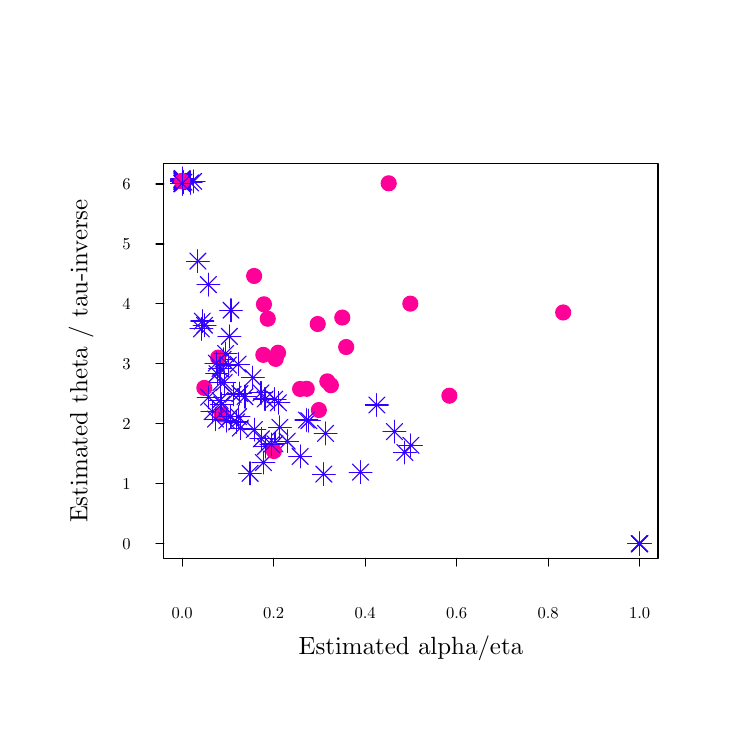
\begin{tikzpicture}[x=1pt,y=1pt]
\definecolor{fillColor}{RGB}{255,255,255}
\path[use as bounding box,fill=fillColor,fill opacity=0.00] (0,0) rectangle (252.94,252.94);
\begin{scope}
\path[clip] ( 49.20, 61.20) rectangle (227.75,203.75);
\definecolor{drawColor}{RGB}{51,0,255}

\path[draw=drawColor,line width= 0.4pt,line join=round,line cap=round] ( 62.35,157.19) -- ( 68.20,163.04);

\path[draw=drawColor,line width= 0.4pt,line join=round,line cap=round] ( 62.35,163.04) -- ( 68.20,157.19);

\path[draw=drawColor,line width= 0.4pt,line join=round,line cap=round] ( 61.14,160.12) -- ( 69.41,160.12);

\path[draw=drawColor,line width= 0.4pt,line join=round,line cap=round] ( 65.27,155.98) -- ( 65.27,164.25);

\path[draw=drawColor,line width= 0.4pt,line join=round,line cap=round] ( 67.72,130.20) -- ( 73.57,136.05);

\path[draw=drawColor,line width= 0.4pt,line join=round,line cap=round] ( 67.72,136.05) -- ( 73.57,130.20);

\path[draw=drawColor,line width= 0.4pt,line join=round,line cap=round] ( 66.51,133.12) -- ( 74.79,133.12);

\path[draw=drawColor,line width= 0.4pt,line join=round,line cap=round] ( 70.65,128.99) -- ( 70.65,137.26);

\path[draw=drawColor,line width= 0.4pt,line join=round,line cap=round] (218.21, 63.55) -- (224.06, 69.40);

\path[draw=drawColor,line width= 0.4pt,line join=round,line cap=round] (218.21, 69.40) -- (224.06, 63.55);

\path[draw=drawColor,line width= 0.4pt,line join=round,line cap=round] (217.00, 66.48) -- (225.27, 66.48);

\path[draw=drawColor,line width= 0.4pt,line join=round,line cap=round] (221.13, 62.34) -- (221.13, 70.62);
\definecolor{fillColor}{RGB}{255,0,153}

\path[fill=fillColor] (109.56,123.73) circle (  2.92);

\path[draw=drawColor,line width= 0.4pt,line join=round,line cap=round] ( 81.38,118.06) -- ( 87.23,123.91);

\path[draw=drawColor,line width= 0.4pt,line join=round,line cap=round] ( 81.38,123.91) -- ( 87.23,118.06);

\path[draw=drawColor,line width= 0.4pt,line join=round,line cap=round] ( 80.17,120.99) -- ( 88.44,120.99);

\path[draw=drawColor,line width= 0.4pt,line join=round,line cap=round] ( 84.30,116.85) -- ( 84.30,125.12);

\path[fill=fillColor] ( 63.83,122.76) circle (  2.92);

\path[draw=drawColor,line width= 0.4pt,line join=round,line cap=round] ( 86.43, 99.65) -- ( 92.28,105.50);

\path[draw=drawColor,line width= 0.4pt,line join=round,line cap=round] ( 86.43,105.50) -- ( 92.28, 99.65);

\path[draw=drawColor,line width= 0.4pt,line join=round,line cap=round] ( 85.22,102.57) -- ( 93.49,102.57);

\path[draw=drawColor,line width= 0.4pt,line join=round,line cap=round] ( 89.36, 98.44) -- ( 89.36,106.71);

\path[fill=fillColor] (130.46,196.70) circle (  2.92);

\path[draw=drawColor,line width= 0.4pt,line join=round,line cap=round] ( 87.66,114.47) -- ( 93.51,120.32);

\path[draw=drawColor,line width= 0.4pt,line join=round,line cap=round] ( 87.66,120.32) -- ( 93.51,114.47);

\path[draw=drawColor,line width= 0.4pt,line join=round,line cap=round] ( 86.45,117.40) -- ( 94.72,117.40);

\path[draw=drawColor,line width= 0.4pt,line join=round,line cap=round] ( 90.59,113.26) -- ( 90.59,121.53);

\path[fill=fillColor] ( 68.83,133.69) circle (  2.92);

\path[draw=drawColor,line width= 0.4pt,line join=round,line cap=round] ( 52.89,194.48) -- ( 58.74,200.33);

\path[draw=drawColor,line width= 0.4pt,line join=round,line cap=round] ( 52.89,200.33) -- ( 58.74,194.48);

\path[draw=drawColor,line width= 0.4pt,line join=round,line cap=round] ( 51.68,197.41) -- ( 59.95,197.41);

\path[draw=drawColor,line width= 0.4pt,line join=round,line cap=round] ( 55.81,193.27) -- ( 55.81,201.54);

\path[draw=drawColor,line width= 0.4pt,line join=round,line cap=round] ( 81.54,101.44) -- ( 87.39,107.29);

\path[draw=drawColor,line width= 0.4pt,line join=round,line cap=round] ( 81.54,107.29) -- ( 87.39,101.44);

\path[draw=drawColor,line width= 0.4pt,line join=round,line cap=round] ( 80.33,104.36) -- ( 88.60,104.36);

\path[draw=drawColor,line width= 0.4pt,line join=round,line cap=round] ( 84.47,100.23) -- ( 84.47,108.50);

\path[draw=drawColor,line width= 0.4pt,line join=round,line cap=round] ( 53.52,194.19) -- ( 59.37,200.04);

\path[draw=drawColor,line width= 0.4pt,line join=round,line cap=round] ( 53.52,200.04) -- ( 59.37,194.19);

\path[draw=drawColor,line width= 0.4pt,line join=round,line cap=round] ( 52.31,197.12) -- ( 60.59,197.12);

\path[draw=drawColor,line width= 0.4pt,line join=round,line cap=round] ( 56.45,192.98) -- ( 56.45,201.25);

\path[draw=drawColor,line width= 0.4pt,line join=round,line cap=round] ( 71.31,117.52) -- ( 77.16,123.37);

\path[draw=drawColor,line width= 0.4pt,line join=round,line cap=round] ( 71.31,123.37) -- ( 77.16,117.52);

\path[draw=drawColor,line width= 0.4pt,line join=round,line cap=round] ( 70.09,120.45) -- ( 78.37,120.45);

\path[draw=drawColor,line width= 0.4pt,line join=round,line cap=round] ( 74.23,116.31) -- ( 74.23,124.58);

\path[draw=drawColor,line width= 0.4pt,line join=round,line cap=round] ( 52.89,194.63) -- ( 58.74,200.48);

\path[draw=drawColor,line width= 0.4pt,line join=round,line cap=round] ( 52.89,200.48) -- ( 58.74,194.63);

\path[draw=drawColor,line width= 0.4pt,line join=round,line cap=round] ( 51.68,197.56) -- ( 59.95,197.56);

\path[draw=drawColor,line width= 0.4pt,line join=round,line cap=round] ( 55.81,193.42) -- ( 55.81,201.69);

\path[draw=drawColor,line width= 0.4pt,line join=round,line cap=round] ( 52.89,194.60) -- ( 58.74,200.45);

\path[draw=drawColor,line width= 0.4pt,line join=round,line cap=round] ( 52.89,200.45) -- ( 58.74,194.60);

\path[draw=drawColor,line width= 0.4pt,line join=round,line cap=round] ( 51.68,197.52) -- ( 59.95,197.52);

\path[draw=drawColor,line width= 0.4pt,line join=round,line cap=round] ( 55.81,193.39) -- ( 55.81,201.66);

\path[fill=fillColor] (104.82,145.86) circle (  2.92);

\path[draw=drawColor,line width= 0.4pt,line join=round,line cap=round] ( 62.47,116.50) -- ( 68.32,122.35);

\path[draw=drawColor,line width= 0.4pt,line join=round,line cap=round] ( 62.47,122.35) -- ( 68.32,116.50);

\path[draw=drawColor,line width= 0.4pt,line join=round,line cap=round] ( 61.26,119.43) -- ( 69.53,119.43);

\path[draw=drawColor,line width= 0.4pt,line join=round,line cap=round] ( 65.40,115.29) -- ( 65.40,123.56);

\path[draw=drawColor,line width= 0.4pt,line join=round,line cap=round] ( 98.67,108.01) -- (104.52,113.86);

\path[draw=drawColor,line width= 0.4pt,line join=round,line cap=round] ( 98.67,113.86) -- (104.52,108.01);

\path[draw=drawColor,line width= 0.4pt,line join=round,line cap=round] ( 97.45,110.93) -- (105.73,110.93);

\path[draw=drawColor,line width= 0.4pt,line join=round,line cap=round] (101.59,106.80) -- (101.59,115.07);

\path[draw=drawColor,line width= 0.4pt,line join=round,line cap=round] ( 52.89,193.75) -- ( 58.74,199.60);

\path[draw=drawColor,line width= 0.4pt,line join=round,line cap=round] ( 52.89,199.60) -- ( 58.74,193.75);

\path[draw=drawColor,line width= 0.4pt,line join=round,line cap=round] ( 51.68,196.68) -- ( 59.95,196.68);

\path[draw=drawColor,line width= 0.4pt,line join=round,line cap=round] ( 55.81,192.54) -- ( 55.81,200.81);

\path[draw=drawColor,line width= 0.4pt,line join=round,line cap=round] (218.09, 63.55) -- (223.94, 69.40);

\path[draw=drawColor,line width= 0.4pt,line join=round,line cap=round] (218.09, 69.40) -- (223.94, 63.55);

\path[draw=drawColor,line width= 0.4pt,line join=round,line cap=round] (216.88, 66.48) -- (225.15, 66.48);

\path[draw=drawColor,line width= 0.4pt,line join=round,line cap=round] (221.01, 62.34) -- (221.01, 70.62);

\path[draw=drawColor,line width= 0.4pt,line join=round,line cap=round] ( 73.76,117.78) -- ( 79.61,123.63);

\path[draw=drawColor,line width= 0.4pt,line join=round,line cap=round] ( 73.76,123.63) -- ( 79.61,117.78);

\path[draw=drawColor,line width= 0.4pt,line join=round,line cap=round] ( 72.54,120.70) -- ( 80.82,120.70);

\path[draw=drawColor,line width= 0.4pt,line join=round,line cap=round] ( 76.68,116.57) -- ( 76.68,124.84);

\path[draw=drawColor,line width= 0.4pt,line join=round,line cap=round] ( 66.57,126.82) -- ( 72.42,132.67);

\path[draw=drawColor,line width= 0.4pt,line join=round,line cap=round] ( 66.57,132.67) -- ( 72.42,126.82);

\path[draw=drawColor,line width= 0.4pt,line join=round,line cap=round] ( 65.36,129.74) -- ( 73.63,129.74);

\path[draw=drawColor,line width= 0.4pt,line join=round,line cap=round] ( 69.50,125.61) -- ( 69.50,133.88);

\path[draw=drawColor,line width= 0.4pt,line join=round,line cap=round] ( 52.89,195.54) -- ( 58.74,201.39);

\path[draw=drawColor,line width= 0.4pt,line join=round,line cap=round] ( 52.89,201.39) -- ( 58.74,195.54);

\path[draw=drawColor,line width= 0.4pt,line join=round,line cap=round] ( 51.68,198.47) -- ( 59.95,198.47);

\path[draw=drawColor,line width= 0.4pt,line join=round,line cap=round] ( 55.81,194.33) -- ( 55.81,202.60);

\path[draw=drawColor,line width= 0.4pt,line join=round,line cap=round] ( 63.79,111.31) -- ( 69.64,117.16);

\path[draw=drawColor,line width= 0.4pt,line join=round,line cap=round] ( 63.79,117.16) -- ( 69.64,111.31);

\path[draw=drawColor,line width= 0.4pt,line join=round,line cap=round] ( 62.57,114.23) -- ( 70.85,114.23);

\path[draw=drawColor,line width= 0.4pt,line join=round,line cap=round] ( 66.71,110.10) -- ( 66.71,118.37);

\path[fill=fillColor] ( 55.81,197.59) circle (  2.92);

\path[draw=drawColor,line width= 0.4pt,line join=round,line cap=round] ( 58.59,165.67) -- ( 64.44,171.52);

\path[draw=drawColor,line width= 0.4pt,line join=round,line cap=round] ( 58.59,171.52) -- ( 64.44,165.67);

\path[draw=drawColor,line width= 0.4pt,line join=round,line cap=round] ( 57.38,168.59) -- ( 65.66,168.59);

\path[draw=drawColor,line width= 0.4pt,line join=round,line cap=round] ( 61.52,164.45) -- ( 61.52,172.73);

\path[draw=drawColor,line width= 0.4pt,line join=round,line cap=round] (218.21, 63.55) -- (224.06, 69.40);

\path[draw=drawColor,line width= 0.4pt,line join=round,line cap=round] (218.21, 69.40) -- (224.06, 63.55);

\path[draw=drawColor,line width= 0.4pt,line join=round,line cap=round] (217.00, 66.48) -- (225.27, 66.48);

\path[draw=drawColor,line width= 0.4pt,line join=round,line cap=round] (221.13, 62.34) -- (221.13, 70.62);

\path[draw=drawColor,line width= 0.4pt,line join=round,line cap=round] ( 60.98,142.48) -- ( 66.83,148.33);

\path[draw=drawColor,line width= 0.4pt,line join=round,line cap=round] ( 60.98,148.33) -- ( 66.83,142.48);

\path[draw=drawColor,line width= 0.4pt,line join=round,line cap=round] ( 59.77,145.41) -- ( 68.04,145.41);

\path[draw=drawColor,line width= 0.4pt,line join=round,line cap=round] ( 63.90,141.27) -- ( 63.90,149.55);

\path[draw=drawColor,line width= 0.4pt,line join=round,line cap=round] ( 86.33,115.77) -- ( 92.18,121.62);

\path[draw=drawColor,line width= 0.4pt,line join=round,line cap=round] ( 86.33,121.62) -- ( 92.18,115.77);

\path[draw=drawColor,line width= 0.4pt,line join=round,line cap=round] ( 85.12,118.70) -- ( 93.39,118.70);

\path[draw=drawColor,line width= 0.4pt,line join=round,line cap=round] ( 89.26,114.56) -- ( 89.26,122.83);

\path[draw=drawColor,line width= 0.4pt,line join=round,line cap=round] ( 78.46,123.54) -- ( 84.31,129.39);

\path[draw=drawColor,line width= 0.4pt,line join=round,line cap=round] ( 78.46,129.39) -- ( 84.31,123.54);

\path[draw=drawColor,line width= 0.4pt,line join=round,line cap=round] ( 77.24,126.46) -- ( 85.52,126.46);

\path[draw=drawColor,line width= 0.4pt,line join=round,line cap=round] ( 81.38,122.33) -- ( 81.38,130.60);

\path[draw=drawColor,line width= 0.4pt,line join=round,line cap=round] ( 72.59,107.54) -- ( 78.44,113.39);

\path[draw=drawColor,line width= 0.4pt,line join=round,line cap=round] ( 72.59,113.39) -- ( 78.44,107.54);

\path[draw=drawColor,line width= 0.4pt,line join=round,line cap=round] ( 71.38,110.46) -- ( 79.65,110.46);

\path[draw=drawColor,line width= 0.4pt,line join=round,line cap=round] ( 75.51,106.33) -- ( 75.51,114.60);

\path[draw=drawColor,line width= 0.4pt,line join=round,line cap=round] ( 82.96, 98.61) -- ( 88.81,104.46);

\path[draw=drawColor,line width= 0.4pt,line join=round,line cap=round] ( 82.96,104.46) -- ( 88.81, 98.61);

\path[draw=drawColor,line width= 0.4pt,line join=round,line cap=round] ( 81.75,101.53) -- ( 90.02,101.53);

\path[draw=drawColor,line width= 0.4pt,line join=round,line cap=round] ( 85.88, 97.39) -- ( 85.88,105.67);

\path[draw=drawColor,line width= 0.4pt,line join=round,line cap=round] ( 69.96,138.46) -- ( 75.81,144.31);

\path[draw=drawColor,line width= 0.4pt,line join=round,line cap=round] ( 69.96,144.31) -- ( 75.81,138.46);

\path[draw=drawColor,line width= 0.4pt,line join=round,line cap=round] ( 68.75,141.38) -- ( 77.03,141.38);

\path[draw=drawColor,line width= 0.4pt,line join=round,line cap=round] ( 72.89,137.24) -- ( 72.89,145.52);

\path[draw=drawColor,line width= 0.4pt,line join=round,line cap=round] (104.09, 88.70) -- (109.94, 94.55);

\path[draw=drawColor,line width= 0.4pt,line join=round,line cap=round] (104.09, 94.55) -- (109.94, 88.70);

\path[draw=drawColor,line width= 0.4pt,line join=round,line cap=round] (102.88, 91.62) -- (111.15, 91.62);

\path[draw=drawColor,line width= 0.4pt,line join=round,line cap=round] (107.02, 87.48) -- (107.02, 95.76);

\path[draw=drawColor,line width= 0.4pt,line join=round,line cap=round] (218.21, 63.55) -- (224.06, 69.40);

\path[draw=drawColor,line width= 0.4pt,line join=round,line cap=round] (218.21, 69.40) -- (224.06, 63.55);

\path[draw=drawColor,line width= 0.4pt,line join=round,line cap=round] (217.00, 66.48) -- (225.27, 66.48);

\path[draw=drawColor,line width= 0.4pt,line join=round,line cap=round] (221.13, 62.34) -- (221.13, 70.62);

\path[fill=fillColor] (105.22,114.77) circle (  2.92);

\path[draw=drawColor,line width= 0.4pt,line join=round,line cap=round] ( 52.89,195.12) -- ( 58.74,200.97);

\path[draw=drawColor,line width= 0.4pt,line join=round,line cap=round] ( 52.89,200.97) -- ( 58.74,195.12);

\path[draw=drawColor,line width= 0.4pt,line join=round,line cap=round] ( 51.68,198.04) -- ( 59.95,198.04);

\path[draw=drawColor,line width= 0.4pt,line join=round,line cap=round] ( 55.81,193.90) -- ( 55.81,202.18);

\path[draw=drawColor,line width= 0.4pt,line join=round,line cap=round] (117.35, 89.42) -- (123.20, 95.27);

\path[draw=drawColor,line width= 0.4pt,line join=round,line cap=round] (117.35, 95.27) -- (123.20, 89.42);

\path[draw=drawColor,line width= 0.4pt,line join=round,line cap=round] (116.13, 92.35) -- (124.41, 92.35);

\path[draw=drawColor,line width= 0.4pt,line join=round,line cap=round] (120.27, 88.21) -- (120.27, 96.48);

\path[draw=drawColor,line width= 0.4pt,line join=round,line cap=round] (133.40, 96.50) -- (139.25,102.35);

\path[draw=drawColor,line width= 0.4pt,line join=round,line cap=round] (133.40,102.35) -- (139.25, 96.50);

\path[draw=drawColor,line width= 0.4pt,line join=round,line cap=round] (132.18, 99.42) -- (140.46, 99.42);

\path[draw=drawColor,line width= 0.4pt,line join=round,line cap=round] (136.32, 95.29) -- (136.32,103.56);

\path[draw=drawColor,line width= 0.4pt,line join=round,line cap=round] ( 68.06,121.82) -- ( 73.91,127.67);

\path[draw=drawColor,line width= 0.4pt,line join=round,line cap=round] ( 68.06,127.67) -- ( 73.91,121.82);

\path[draw=drawColor,line width= 0.4pt,line join=round,line cap=round] ( 66.85,124.75) -- ( 75.12,124.75);

\path[draw=drawColor,line width= 0.4pt,line join=round,line cap=round] ( 70.98,120.61) -- ( 70.98,128.89);

\path[draw=drawColor,line width= 0.4pt,line join=round,line cap=round] ( 69.59,128.11) -- ( 75.44,133.96);

\path[draw=drawColor,line width= 0.4pt,line join=round,line cap=round] ( 69.59,133.96) -- ( 75.44,128.11);

\path[draw=drawColor,line width= 0.4pt,line join=round,line cap=round] ( 68.38,131.03) -- ( 76.65,131.03);

\path[draw=drawColor,line width= 0.4pt,line join=round,line cap=round] ( 72.52,126.89) -- ( 72.52,135.17);

\path[draw=drawColor,line width= 0.4pt,line join=round,line cap=round] ( 52.89,194.32) -- ( 58.74,200.17);

\path[draw=drawColor,line width= 0.4pt,line join=round,line cap=round] ( 52.89,200.17) -- ( 58.74,194.32);

\path[draw=drawColor,line width= 0.4pt,line join=round,line cap=round] ( 51.68,197.25) -- ( 59.95,197.25);

\path[draw=drawColor,line width= 0.4pt,line join=round,line cap=round] ( 55.81,193.11) -- ( 55.81,201.38);

\path[draw=drawColor,line width= 0.4pt,line join=round,line cap=round] ( 52.89,195.15) -- ( 58.74,201.00);

\path[draw=drawColor,line width= 0.4pt,line join=round,line cap=round] ( 52.89,201.00) -- ( 58.74,195.15);

\path[draw=drawColor,line width= 0.4pt,line join=round,line cap=round] ( 51.68,198.08) -- ( 59.95,198.08);

\path[draw=drawColor,line width= 0.4pt,line join=round,line cap=round] ( 55.81,193.94) -- ( 55.81,202.21);

\path[draw=drawColor,line width= 0.4pt,line join=round,line cap=round] ( 73.09,128.44) -- ( 78.94,134.29);

\path[draw=drawColor,line width= 0.4pt,line join=round,line cap=round] ( 73.09,134.29) -- ( 78.94,128.44);

\path[draw=drawColor,line width= 0.4pt,line join=round,line cap=round] ( 71.88,131.37) -- ( 80.16,131.37);

\path[draw=drawColor,line width= 0.4pt,line join=round,line cap=round] ( 76.02,127.23) -- ( 76.02,135.50);

\path[draw=drawColor,line width= 0.4pt,line join=round,line cap=round] ( 90.84,100.61) -- ( 96.69,106.46);

\path[draw=drawColor,line width= 0.4pt,line join=round,line cap=round] ( 90.84,106.46) -- ( 96.69,100.61);

\path[draw=drawColor,line width= 0.4pt,line join=round,line cap=round] ( 89.63,103.53) -- ( 97.90,103.53);

\path[draw=drawColor,line width= 0.4pt,line join=round,line cap=round] ( 93.76, 99.39) -- ( 93.76,107.67);

\path[fill=fillColor] ( 89.62,133.25) circle (  2.92);

\path[fill=fillColor] (138.27,153.21) circle (  2.92);

\path[draw=drawColor,line width= 0.4pt,line join=round,line cap=round] (123.23,113.67) -- (129.08,119.52);

\path[draw=drawColor,line width= 0.4pt,line join=round,line cap=round] (123.23,119.52) -- (129.08,113.67);

\path[draw=drawColor,line width= 0.4pt,line join=round,line cap=round] (122.02,116.59) -- (130.29,116.59);

\path[draw=drawColor,line width= 0.4pt,line join=round,line cap=round] (126.16,112.45) -- (126.16,120.73);

\path[draw=drawColor,line width= 0.4pt,line join=round,line cap=round] ( 52.89,195.02) -- ( 58.74,200.87);

\path[draw=drawColor,line width= 0.4pt,line join=round,line cap=round] ( 52.89,200.87) -- ( 58.74,195.02);

\path[draw=drawColor,line width= 0.4pt,line join=round,line cap=round] ( 51.68,197.94) -- ( 59.95,197.94);

\path[draw=drawColor,line width= 0.4pt,line join=round,line cap=round] ( 55.81,193.81) -- ( 55.81,202.08);

\path[fill=fillColor] ( 81.83,163.22) circle (  2.92);

\path[fill=fillColor] ( 70.07,113.18) circle (  2.92);

\path[draw=drawColor,line width= 0.4pt,line join=round,line cap=round] ( 52.89,195.23) -- ( 58.74,201.08);

\path[draw=drawColor,line width= 0.4pt,line join=round,line cap=round] ( 52.89,201.08) -- ( 58.74,195.23);

\path[draw=drawColor,line width= 0.4pt,line join=round,line cap=round] ( 51.68,198.16) -- ( 59.95,198.16);

\path[draw=drawColor,line width= 0.4pt,line join=round,line cap=round] ( 55.81,194.02) -- ( 55.81,202.29);

\path[fill=fillColor] (108.27,125.13) circle (  2.92);

\path[fill=fillColor] (193.50,150.03) circle (  2.92);

\path[draw=drawColor,line width= 0.4pt,line join=round,line cap=round] ( 52.89,193.58) -- ( 58.74,199.43);

\path[draw=drawColor,line width= 0.4pt,line join=round,line cap=round] ( 52.89,199.43) -- ( 58.74,193.58);

\path[draw=drawColor,line width= 0.4pt,line join=round,line cap=round] ( 51.68,196.50) -- ( 59.95,196.50);

\path[draw=drawColor,line width= 0.4pt,line join=round,line cap=round] ( 55.81,192.36) -- ( 55.81,200.64);

\path[draw=drawColor,line width= 0.4pt,line join=round,line cap=round] ( 82.27, 92.88) -- ( 88.12, 98.73);

\path[draw=drawColor,line width= 0.4pt,line join=round,line cap=round] ( 82.27, 98.73) -- ( 88.12, 92.88);

\path[draw=drawColor,line width= 0.4pt,line join=round,line cap=round] ( 81.05, 95.80) -- ( 89.33, 95.80);

\path[draw=drawColor,line width= 0.4pt,line join=round,line cap=round] ( 85.19, 91.67) -- ( 85.19, 99.94);

\path[draw=drawColor,line width= 0.4pt,line join=round,line cap=round] ( 59.84,141.16) -- ( 65.69,147.01);

\path[draw=drawColor,line width= 0.4pt,line join=round,line cap=round] ( 59.84,147.01) -- ( 65.69,141.16);

\path[draw=drawColor,line width= 0.4pt,line join=round,line cap=round] ( 58.63,144.08) -- ( 66.90,144.08);

\path[draw=drawColor,line width= 0.4pt,line join=round,line cap=round] ( 62.77,139.95) -- ( 62.77,148.22);

\path[draw=drawColor,line width= 0.4pt,line join=round,line cap=round] ( 57.06,194.49) -- ( 62.91,200.34);

\path[draw=drawColor,line width= 0.4pt,line join=round,line cap=round] ( 57.06,200.34) -- ( 62.91,194.49);

\path[draw=drawColor,line width= 0.4pt,line join=round,line cap=round] ( 55.85,197.41) -- ( 64.12,197.41);

\path[draw=drawColor,line width= 0.4pt,line join=round,line cap=round] ( 59.99,193.28) -- ( 59.99,201.55);

\path[draw=drawColor,line width= 0.4pt,line join=round,line cap=round] (218.21, 63.55) -- (224.06, 69.40);

\path[draw=drawColor,line width= 0.4pt,line join=round,line cap=round] (218.21, 69.40) -- (224.06, 63.55);

\path[draw=drawColor,line width= 0.4pt,line join=round,line cap=round] (217.00, 66.48) -- (225.27, 66.48);

\path[draw=drawColor,line width= 0.4pt,line join=round,line cap=round] (221.13, 62.34) -- (221.13, 70.62);

\path[fill=fillColor] ( 90.47,135.47) circle (  2.92);

\path[fill=fillColor] ( 88.97, 99.96) circle (  2.92);

\path[draw=drawColor,line width= 0.4pt,line join=round,line cap=round] ( 77.42, 88.99) -- ( 83.27, 94.84);

\path[draw=drawColor,line width= 0.4pt,line join=round,line cap=round] ( 77.42, 94.84) -- ( 83.27, 88.99);

\path[draw=drawColor,line width= 0.4pt,line join=round,line cap=round] ( 76.20, 91.92) -- ( 84.48, 91.92);

\path[draw=drawColor,line width= 0.4pt,line join=round,line cap=round] ( 80.34, 87.78) -- ( 80.34, 96.05);

\path[draw=drawColor,line width= 0.4pt,line join=round,line cap=round] (218.09, 63.55) -- (223.94, 69.40);

\path[draw=drawColor,line width= 0.4pt,line join=round,line cap=round] (218.09, 69.40) -- (223.94, 63.55);

\path[draw=drawColor,line width= 0.4pt,line join=round,line cap=round] (216.88, 66.48) -- (225.15, 66.48);

\path[draw=drawColor,line width= 0.4pt,line join=round,line cap=round] (221.01, 62.34) -- (221.01, 70.62);

\path[draw=drawColor,line width= 0.4pt,line join=round,line cap=round] ( 73.26,109.43) -- ( 79.11,115.28);

\path[draw=drawColor,line width= 0.4pt,line join=round,line cap=round] ( 73.26,115.28) -- ( 79.11,109.43);

\path[draw=drawColor,line width= 0.4pt,line join=round,line cap=round] ( 72.05,112.36) -- ( 80.32,112.36);

\path[draw=drawColor,line width= 0.4pt,line join=round,line cap=round] ( 76.18,108.22) -- ( 76.18,116.49);

\path[draw=drawColor,line width= 0.4pt,line join=round,line cap=round] ( 88.22,105.63) -- ( 94.07,111.48);

\path[draw=drawColor,line width= 0.4pt,line join=round,line cap=round] ( 88.22,111.48) -- ( 94.07,105.63);

\path[draw=drawColor,line width= 0.4pt,line join=round,line cap=round] ( 87.01,108.55) -- ( 95.28,108.55);

\path[draw=drawColor,line width= 0.4pt,line join=round,line cap=round] ( 91.14,104.42) -- ( 91.14,112.69);

\path[draw=drawColor,line width= 0.4pt,line join=round,line cap=round] ( 82.84,115.83) -- ( 88.69,121.68);

\path[draw=drawColor,line width= 0.4pt,line join=round,line cap=round] ( 82.84,121.68) -- ( 88.69,115.83);

\path[draw=drawColor,line width= 0.4pt,line join=round,line cap=round] ( 81.63,118.76) -- ( 89.90,118.76);

\path[draw=drawColor,line width= 0.4pt,line join=round,line cap=round] ( 85.77,114.62) -- ( 85.77,122.89);

\path[draw=drawColor,line width= 0.4pt,line join=round,line cap=round] ( 52.89,193.74) -- ( 58.74,199.59);

\path[draw=drawColor,line width= 0.4pt,line join=round,line cap=round] ( 52.89,199.59) -- ( 58.74,193.74);

\path[draw=drawColor,line width= 0.4pt,line join=round,line cap=round] ( 51.68,196.67) -- ( 59.95,196.67);

\path[draw=drawColor,line width= 0.4pt,line join=round,line cap=round] ( 55.81,192.53) -- ( 55.81,200.80);

\path[fill=fillColor] (100.83,122.44) circle (  2.92);

\path[draw=drawColor,line width= 0.4pt,line join=round,line cap=round] ( 78.97,104.76) -- ( 84.82,110.61);

\path[draw=drawColor,line width= 0.4pt,line join=round,line cap=round] ( 78.97,110.61) -- ( 84.82,104.76);

\path[draw=drawColor,line width= 0.4pt,line join=round,line cap=round] ( 77.75,107.68) -- ( 86.03,107.68);

\path[draw=drawColor,line width= 0.4pt,line join=round,line cap=round] ( 81.89,103.55) -- ( 81.89,111.82);

\path[draw=drawColor,line width= 0.4pt,line join=round,line cap=round] ( 73.91,105.31) -- ( 79.76,111.16);

\path[draw=drawColor,line width= 0.4pt,line join=round,line cap=round] ( 73.91,111.16) -- ( 79.76,105.31);

\path[draw=drawColor,line width= 0.4pt,line join=round,line cap=round] ( 72.70,108.23) -- ( 80.98,108.23);

\path[draw=drawColor,line width= 0.4pt,line join=round,line cap=round] ( 76.84,104.10) -- ( 76.84,112.37);

\path[fill=fillColor] ( 86.75,147.75) circle (  2.92);

\path[fill=fillColor] ( 98.44,122.39) circle (  2.92);

\path[draw=drawColor,line width= 0.4pt,line join=round,line cap=round] ( 75.60,116.66) -- ( 81.45,122.51);

\path[draw=drawColor,line width= 0.4pt,line join=round,line cap=round] ( 75.60,122.51) -- ( 81.45,116.66);

\path[draw=drawColor,line width= 0.4pt,line join=round,line cap=round] ( 74.39,119.58) -- ( 82.66,119.58);

\path[draw=drawColor,line width= 0.4pt,line join=round,line cap=round] ( 78.53,115.45) -- ( 78.53,123.72);

\path[fill=fillColor] (115.09,137.54) circle (  2.92);

\path[draw=drawColor,line width= 0.4pt,line join=round,line cap=round] ( 52.89,193.82) -- ( 58.74,199.67);

\path[draw=drawColor,line width= 0.4pt,line join=round,line cap=round] ( 52.89,199.67) -- ( 58.74,193.82);

\path[draw=drawColor,line width= 0.4pt,line join=round,line cap=round] ( 51.68,196.75) -- ( 59.95,196.75);

\path[draw=drawColor,line width= 0.4pt,line join=round,line cap=round] ( 55.81,192.61) -- ( 55.81,200.89);

\path[draw=drawColor,line width= 0.4pt,line join=round,line cap=round] (135.56, 99.11) -- (141.41,104.96);

\path[draw=drawColor,line width= 0.4pt,line join=round,line cap=round] (135.56,104.96) -- (141.41, 99.11);

\path[draw=drawColor,line width= 0.4pt,line join=round,line cap=round] (134.35,102.03) -- (142.62,102.03);

\path[draw=drawColor,line width= 0.4pt,line join=round,line cap=round] (138.48, 97.90) -- (138.48,106.17);

\path[draw=drawColor,line width= 0.4pt,line join=round,line cap=round] ( 64.94,108.57) -- ( 70.79,114.42);

\path[draw=drawColor,line width= 0.4pt,line join=round,line cap=round] ( 64.94,114.42) -- ( 70.79,108.57);

\path[draw=drawColor,line width= 0.4pt,line join=round,line cap=round] ( 63.73,111.49) -- ( 72.00,111.49);

\path[draw=drawColor,line width= 0.4pt,line join=round,line cap=round] ( 67.86,107.36) -- ( 67.86,115.63);

\path[draw=drawColor,line width= 0.4pt,line join=round,line cap=round] ( 70.55,147.91) -- ( 76.40,153.76);

\path[draw=drawColor,line width= 0.4pt,line join=round,line cap=round] ( 70.55,153.76) -- ( 76.40,147.91);

\path[draw=drawColor,line width= 0.4pt,line join=round,line cap=round] ( 69.34,150.84) -- ( 77.61,150.84);

\path[draw=drawColor,line width= 0.4pt,line join=round,line cap=round] ( 73.48,146.70) -- ( 73.48,154.97);

\path[draw=drawColor,line width= 0.4pt,line join=round,line cap=round] ( 52.89,194.62) -- ( 58.74,200.47);

\path[draw=drawColor,line width= 0.4pt,line join=round,line cap=round] ( 52.89,200.47) -- ( 58.74,194.62);

\path[draw=drawColor,line width= 0.4pt,line join=round,line cap=round] ( 51.68,197.55) -- ( 59.95,197.55);

\path[draw=drawColor,line width= 0.4pt,line join=round,line cap=round] ( 55.81,193.41) -- ( 55.81,201.68);

\path[draw=drawColor,line width= 0.4pt,line join=round,line cap=round] ( 70.24,109.46) -- ( 76.09,115.31);

\path[draw=drawColor,line width= 0.4pt,line join=round,line cap=round] ( 70.24,115.31) -- ( 76.09,109.46);

\path[draw=drawColor,line width= 0.4pt,line join=round,line cap=round] ( 69.03,112.39) -- ( 77.30,112.39);

\path[draw=drawColor,line width= 0.4pt,line join=round,line cap=round] ( 73.17,108.25) -- ( 73.17,116.52);

\path[draw=drawColor,line width= 0.4pt,line join=round,line cap=round] ( 65.22,128.80) -- ( 71.07,134.65);

\path[draw=drawColor,line width= 0.4pt,line join=round,line cap=round] ( 65.22,134.65) -- ( 71.07,128.80);

\path[draw=drawColor,line width= 0.4pt,line join=round,line cap=round] ( 64.01,131.73) -- ( 72.28,131.73);

\path[draw=drawColor,line width= 0.4pt,line join=round,line cap=round] ( 68.14,127.59) -- ( 68.14,135.86);

\path[fill=fillColor] ( 85.15,134.71) circle (  2.92);

\path[draw=drawColor,line width= 0.4pt,line join=round,line cap=round] ( 55.95,193.92) -- ( 61.80,199.77);

\path[draw=drawColor,line width= 0.4pt,line join=round,line cap=round] ( 55.95,199.77) -- ( 61.80,193.92);

\path[draw=drawColor,line width= 0.4pt,line join=round,line cap=round] ( 54.74,196.84) -- ( 63.02,196.84);

\path[draw=drawColor,line width= 0.4pt,line join=round,line cap=round] ( 58.88,192.71) -- ( 58.88,200.98);

\path[fill=fillColor] ( 55.81,197.41) circle (  2.92);

\path[draw=drawColor,line width= 0.4pt,line join=round,line cap=round] ( 52.89,193.71) -- ( 58.74,199.56);

\path[draw=drawColor,line width= 0.4pt,line join=round,line cap=round] ( 52.89,199.56) -- ( 58.74,193.71);

\path[draw=drawColor,line width= 0.4pt,line join=round,line cap=round] ( 51.68,196.63) -- ( 59.95,196.63);

\path[draw=drawColor,line width= 0.4pt,line join=round,line cap=round] ( 55.81,192.50) -- ( 55.81,200.77);

\path[draw=drawColor,line width= 0.4pt,line join=round,line cap=round] ( 67.26,113.96) -- ( 73.11,119.81);

\path[draw=drawColor,line width= 0.4pt,line join=round,line cap=round] ( 67.26,119.81) -- ( 73.11,113.96);

\path[draw=drawColor,line width= 0.4pt,line join=round,line cap=round] ( 66.04,116.89) -- ( 74.32,116.89);

\path[draw=drawColor,line width= 0.4pt,line join=round,line cap=round] ( 70.18,112.75) -- ( 70.18,121.02);

\path[draw=drawColor,line width= 0.4pt,line join=round,line cap=round] ( 85.13, 99.39) -- ( 90.98,105.24);

\path[draw=drawColor,line width= 0.4pt,line join=round,line cap=round] ( 85.13,105.24) -- ( 90.98, 99.39);

\path[draw=drawColor,line width= 0.4pt,line join=round,line cap=round] ( 83.92,102.32) -- ( 92.19,102.32);

\path[draw=drawColor,line width= 0.4pt,line join=round,line cap=round] ( 88.06, 98.18) -- ( 88.06,106.46);

\path[draw=drawColor,line width= 0.4pt,line join=round,line cap=round] (129.61,104.06) -- (135.46,109.91);

\path[draw=drawColor,line width= 0.4pt,line join=round,line cap=round] (129.61,109.91) -- (135.46,104.06);

\path[draw=drawColor,line width= 0.4pt,line join=round,line cap=round] (128.40,106.98) -- (136.67,106.98);

\path[draw=drawColor,line width= 0.4pt,line join=round,line cap=round] (132.53,102.84) -- (132.53,111.12);

\path[draw=drawColor,line width= 0.4pt,line join=round,line cap=round] (104.72,103.41) -- (110.57,109.26);

\path[draw=drawColor,line width= 0.4pt,line join=round,line cap=round] (104.72,109.26) -- (110.57,103.41);

\path[draw=drawColor,line width= 0.4pt,line join=round,line cap=round] (103.51,106.34) -- (111.78,106.34);

\path[draw=drawColor,line width= 0.4pt,line join=round,line cap=round] (107.64,102.20) -- (107.64,110.48);

\path[draw=drawColor,line width= 0.4pt,line join=round,line cap=round] ( 68.59,132.26) -- ( 74.44,138.11);

\path[draw=drawColor,line width= 0.4pt,line join=round,line cap=round] ( 68.59,138.11) -- ( 74.44,132.26);

\path[draw=drawColor,line width= 0.4pt,line join=round,line cap=round] ( 67.38,135.19) -- ( 75.65,135.19);

\path[draw=drawColor,line width= 0.4pt,line join=round,line cap=round] ( 71.51,131.05) -- ( 71.51,139.33);

\path[fill=fillColor] ( 85.38,152.98) circle (  2.92);

\path[draw=drawColor,line width= 0.4pt,line join=round,line cap=round] ( 69.01,108.04) -- ( 74.86,113.89);

\path[draw=drawColor,line width= 0.4pt,line join=round,line cap=round] ( 69.01,113.89) -- ( 74.86,108.04);

\path[draw=drawColor,line width= 0.4pt,line join=round,line cap=round] ( 67.80,110.97) -- ( 76.07,110.97);

\path[draw=drawColor,line width= 0.4pt,line join=round,line cap=round] ( 71.93,106.83) -- ( 71.93,115.11);

\path[fill=fillColor] (113.68,148.19) circle (  2.92);

\path[draw=drawColor,line width= 0.4pt,line join=round,line cap=round] ( 60.16,144.00) -- ( 66.01,149.85);

\path[draw=drawColor,line width= 0.4pt,line join=round,line cap=round] ( 60.16,149.85) -- ( 66.01,144.00);

\path[draw=drawColor,line width= 0.4pt,line join=round,line cap=round] ( 58.95,146.93) -- ( 67.22,146.93);

\path[draw=drawColor,line width= 0.4pt,line join=round,line cap=round] ( 63.09,142.79) -- ( 63.09,151.06);

\path[draw=drawColor,line width= 0.4pt,line join=round,line cap=round] ( 66.60,115.33) -- ( 72.45,121.18);

\path[draw=drawColor,line width= 0.4pt,line join=round,line cap=round] ( 66.60,121.18) -- ( 72.45,115.33);

\path[draw=drawColor,line width= 0.4pt,line join=round,line cap=round] ( 65.39,118.25) -- ( 73.66,118.25);

\path[draw=drawColor,line width= 0.4pt,line join=round,line cap=round] ( 69.53,114.12) -- ( 69.53,122.39);

\path[draw=drawColor,line width= 0.4pt,line join=round,line cap=round] ( 95.54, 95.09) -- (101.39,100.94);

\path[draw=drawColor,line width= 0.4pt,line join=round,line cap=round] ( 95.54,100.94) -- (101.39, 95.09);

\path[draw=drawColor,line width= 0.4pt,line join=round,line cap=round] ( 94.33, 98.02) -- (102.60, 98.02);

\path[draw=drawColor,line width= 0.4pt,line join=round,line cap=round] ( 98.46, 93.88) -- ( 98.46,102.15);

\path[draw=drawColor,line width= 0.4pt,line join=round,line cap=round] ( 97.79,108.25) -- (103.64,114.10);

\path[draw=drawColor,line width= 0.4pt,line join=round,line cap=round] ( 97.79,114.10) -- (103.64,108.25);

\path[draw=drawColor,line width= 0.4pt,line join=round,line cap=round] ( 96.58,111.17) -- (104.85,111.17);

\path[draw=drawColor,line width= 0.4pt,line join=round,line cap=round] (100.71,107.03) -- (100.71,115.31);

\path[fill=fillColor] (152.38,119.95) circle (  2.92);

\path[draw=drawColor,line width= 0.4pt,line join=round,line cap=round] ( 65.51,124.98) -- ( 71.36,130.83);

\path[draw=drawColor,line width= 0.4pt,line join=round,line cap=round] ( 65.51,130.83) -- ( 71.36,124.98);

\path[draw=drawColor,line width= 0.4pt,line join=round,line cap=round] ( 64.30,127.90) -- ( 72.57,127.90);

\path[draw=drawColor,line width= 0.4pt,line join=round,line cap=round] ( 68.44,123.76) -- ( 68.44,132.04);

\path[draw=drawColor,line width= 0.4pt,line join=round,line cap=round] ( 66.91,121.83) -- ( 72.76,127.68);

\path[draw=drawColor,line width= 0.4pt,line join=round,line cap=round] ( 66.91,127.68) -- ( 72.76,121.83);

\path[draw=drawColor,line width= 0.4pt,line join=round,line cap=round] ( 65.70,124.75) -- ( 73.97,124.75);

\path[draw=drawColor,line width= 0.4pt,line join=round,line cap=round] ( 69.83,120.62) -- ( 69.83,128.89);
\end{scope}
\begin{scope}
\path[clip] (  0.00,  0.00) rectangle (252.94,252.94);
\definecolor{drawColor}{RGB}{0,0,0}

\path[draw=drawColor,line width= 0.4pt,line join=round,line cap=round] ( 55.81, 61.20) -- (221.13, 61.20);

\path[draw=drawColor,line width= 0.4pt,line join=round,line cap=round] ( 55.81, 61.20) -- ( 55.81, 58.35);

\path[draw=drawColor,line width= 0.4pt,line join=round,line cap=round] ( 88.88, 61.20) -- ( 88.88, 58.35);

\path[draw=drawColor,line width= 0.4pt,line join=round,line cap=round] (121.94, 61.20) -- (121.94, 58.35);

\path[draw=drawColor,line width= 0.4pt,line join=round,line cap=round] (155.00, 61.20) -- (155.00, 58.35);

\path[draw=drawColor,line width= 0.4pt,line join=round,line cap=round] (188.07, 61.20) -- (188.07, 58.35);

\path[draw=drawColor,line width= 0.4pt,line join=round,line cap=round] (221.13, 61.20) -- (221.13, 58.35);

\node[text=drawColor,anchor=base,inner sep=0pt, outer sep=0pt, scale=  0.60] at ( 55.81, 39.60) {0.0};

\node[text=drawColor,anchor=base,inner sep=0pt, outer sep=0pt, scale=  0.60] at ( 88.88, 39.60) {0.2};

\node[text=drawColor,anchor=base,inner sep=0pt, outer sep=0pt, scale=  0.60] at (121.94, 39.60) {0.4};

\node[text=drawColor,anchor=base,inner sep=0pt, outer sep=0pt, scale=  0.60] at (155.00, 39.60) {0.6};

\node[text=drawColor,anchor=base,inner sep=0pt, outer sep=0pt, scale=  0.60] at (188.07, 39.60) {0.8};

\node[text=drawColor,anchor=base,inner sep=0pt, outer sep=0pt, scale=  0.60] at (221.13, 39.60) {1.0};

\path[draw=drawColor,line width= 0.4pt,line join=round,line cap=round] ( 49.20, 66.48) -- ( 49.20,196.44);

\path[draw=drawColor,line width= 0.4pt,line join=round,line cap=round] ( 49.20, 66.48) -- ( 46.35, 66.48);

\path[draw=drawColor,line width= 0.4pt,line join=round,line cap=round] ( 49.20, 88.14) -- ( 46.35, 88.14);

\path[draw=drawColor,line width= 0.4pt,line join=round,line cap=round] ( 49.20,109.80) -- ( 46.35,109.80);

\path[draw=drawColor,line width= 0.4pt,line join=round,line cap=round] ( 49.20,131.46) -- ( 46.35,131.46);

\path[draw=drawColor,line width= 0.4pt,line join=round,line cap=round] ( 49.20,153.12) -- ( 46.35,153.12);

\path[draw=drawColor,line width= 0.4pt,line join=round,line cap=round] ( 49.20,174.78) -- ( 46.35,174.78);

\path[draw=drawColor,line width= 0.4pt,line join=round,line cap=round] ( 49.20,196.44) -- ( 46.35,196.44);

\node[text=drawColor,anchor=base east,inner sep=0pt, outer sep=0pt, scale=  0.60] at ( 37.20, 64.41) {0};

\node[text=drawColor,anchor=base east,inner sep=0pt, outer sep=0pt, scale=  0.60] at ( 37.20, 86.07) {1};

\node[text=drawColor,anchor=base east,inner sep=0pt, outer sep=0pt, scale=  0.60] at ( 37.20,107.73) {2};

\node[text=drawColor,anchor=base east,inner sep=0pt, outer sep=0pt, scale=  0.60] at ( 37.20,129.40) {3};

\node[text=drawColor,anchor=base east,inner sep=0pt, outer sep=0pt, scale=  0.60] at ( 37.20,151.06) {4};

\node[text=drawColor,anchor=base east,inner sep=0pt, outer sep=0pt, scale=  0.60] at ( 37.20,172.72) {5};

\node[text=drawColor,anchor=base east,inner sep=0pt, outer sep=0pt, scale=  0.60] at ( 37.20,194.38) {6};

\path[draw=drawColor,line width= 0.4pt,line join=round,line cap=round] ( 49.20, 61.20) --
	(227.75, 61.20) --
	(227.75,203.75) --
	( 49.20,203.75) --
	( 49.20, 61.20);
\end{scope}
\begin{scope}
\path[clip] (  0.00,  0.00) rectangle (252.94,252.94);
\definecolor{drawColor}{RGB}{0,0,0}

\node[text=drawColor,anchor=base,inner sep=0pt, outer sep=0pt, scale=  0.90] at (138.47, 26.40) {Estimated alpha/eta};

\node[text=drawColor,rotate= 90.00,anchor=base,inner sep=0pt, outer sep=0pt, scale=  0.90] at ( 21.60,132.47) {Estimated theta / tau-inverse};
\end{scope}
\end{tikzpicture}
 & % Created by tikzDevice version 0.10.1 on 2016-06-29 14:25:44
% !TEX encoding = UTF-8 Unicode
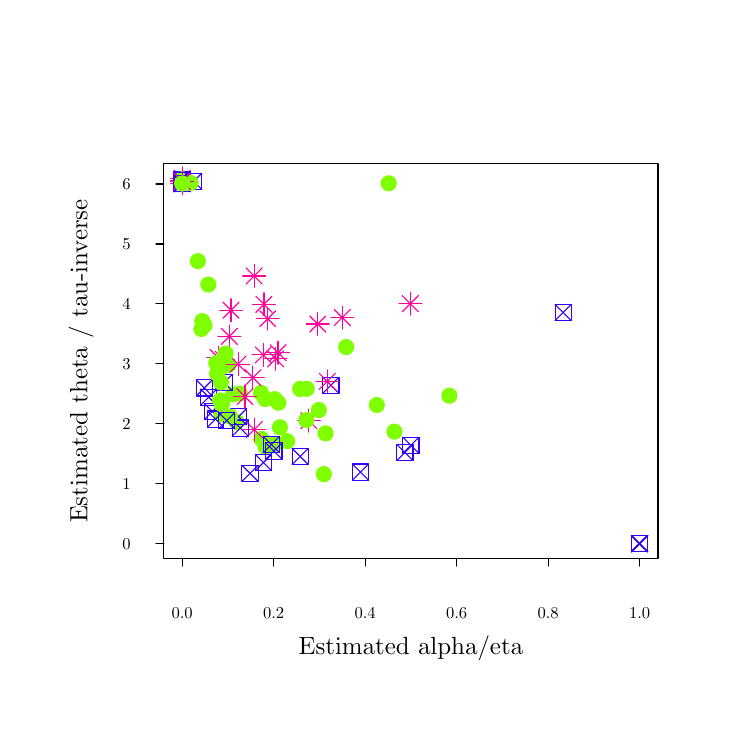
\begin{tikzpicture}[x=1pt,y=1pt]
\definecolor{fillColor}{RGB}{255,255,255}
\path[use as bounding box,fill=fillColor,fill opacity=0.00] (0,0) rectangle (252.94,252.94);
\begin{scope}
\path[clip] ( 49.20, 61.20) rectangle (227.75,203.75);
\definecolor{fillColor}{RGB}{128,255,0}

\path[fill=fillColor] ( 65.27,160.12) circle (  2.92);
\definecolor{drawColor}{RGB}{255,0,153}

\path[draw=drawColor,line width= 0.4pt,line join=round,line cap=round] ( 67.72,130.20) -- ( 73.57,136.05);

\path[draw=drawColor,line width= 0.4pt,line join=round,line cap=round] ( 67.72,136.05) -- ( 73.57,130.20);

\path[draw=drawColor,line width= 0.4pt,line join=round,line cap=round] ( 66.51,133.12) -- ( 74.79,133.12);

\path[draw=drawColor,line width= 0.4pt,line join=round,line cap=round] ( 70.65,128.99) -- ( 70.65,137.26);
\definecolor{drawColor}{RGB}{51,0,255}

\path[draw=drawColor,line width= 0.4pt,line join=round,line cap=round] (218.21, 63.55) rectangle (224.06, 69.40);

\path[draw=drawColor,line width= 0.4pt,line join=round,line cap=round] (218.21, 63.55) -- (224.06, 69.40);

\path[draw=drawColor,line width= 0.4pt,line join=round,line cap=round] (218.21, 69.40) -- (224.06, 63.55);

\path[draw=drawColor,line width= 0.4pt,line join=round,line cap=round] (106.64,120.80) rectangle (112.49,126.65);

\path[draw=drawColor,line width= 0.4pt,line join=round,line cap=round] (106.64,120.80) -- (112.49,126.65);

\path[draw=drawColor,line width= 0.4pt,line join=round,line cap=round] (106.64,126.65) -- (112.49,120.80);

\path[fill=fillColor] ( 84.30,120.99) circle (  2.92);

\path[draw=drawColor,line width= 0.4pt,line join=round,line cap=round] ( 60.90,119.83) rectangle ( 66.75,125.68);

\path[draw=drawColor,line width= 0.4pt,line join=round,line cap=round] ( 60.90,119.83) -- ( 66.75,125.68);

\path[draw=drawColor,line width= 0.4pt,line join=round,line cap=round] ( 60.90,125.68) -- ( 66.75,119.83);

\path[fill=fillColor] ( 89.36,102.57) circle (  2.92);

\path[fill=fillColor] (130.46,196.70) circle (  2.92);

\path[fill=fillColor] ( 90.59,117.40) circle (  2.92);
\definecolor{drawColor}{RGB}{255,0,153}

\path[draw=drawColor,line width= 0.4pt,line join=round,line cap=round] ( 65.90,130.77) -- ( 71.75,136.62);

\path[draw=drawColor,line width= 0.4pt,line join=round,line cap=round] ( 65.90,136.62) -- ( 71.75,130.77);

\path[draw=drawColor,line width= 0.4pt,line join=round,line cap=round] ( 64.69,133.69) -- ( 72.96,133.69);

\path[draw=drawColor,line width= 0.4pt,line join=round,line cap=round] ( 68.83,129.56) -- ( 68.83,137.83);

\path[fill=fillColor] ( 55.81,197.41) circle (  2.92);

\path[fill=fillColor] ( 84.47,104.36) circle (  2.92);

\path[fill=fillColor] ( 56.45,197.12) circle (  2.92);

\path[fill=fillColor] ( 74.23,120.45) circle (  2.92);
\definecolor{drawColor}{RGB}{51,0,255}

\path[draw=drawColor,line width= 0.4pt,line join=round,line cap=round] ( 52.89,194.63) rectangle ( 58.74,200.48);

\path[draw=drawColor,line width= 0.4pt,line join=round,line cap=round] ( 52.89,194.63) -- ( 58.74,200.48);

\path[draw=drawColor,line width= 0.4pt,line join=round,line cap=round] ( 52.89,200.48) -- ( 58.74,194.63);

\path[draw=drawColor,line width= 0.4pt,line join=round,line cap=round] ( 52.89,194.60) rectangle ( 58.74,200.45);

\path[draw=drawColor,line width= 0.4pt,line join=round,line cap=round] ( 52.89,194.60) -- ( 58.74,200.45);

\path[draw=drawColor,line width= 0.4pt,line join=round,line cap=round] ( 52.89,200.45) -- ( 58.74,194.60);
\definecolor{drawColor}{RGB}{255,0,153}

\path[draw=drawColor,line width= 0.4pt,line join=round,line cap=round] (101.89,142.93) -- (107.74,148.78);

\path[draw=drawColor,line width= 0.4pt,line join=round,line cap=round] (101.89,148.78) -- (107.74,142.93);

\path[draw=drawColor,line width= 0.4pt,line join=round,line cap=round] (100.68,145.86) -- (108.95,145.86);

\path[draw=drawColor,line width= 0.4pt,line join=round,line cap=round] (104.82,141.72) -- (104.82,149.99);
\definecolor{drawColor}{RGB}{51,0,255}

\path[draw=drawColor,line width= 0.4pt,line join=round,line cap=round] ( 62.47,116.50) rectangle ( 68.32,122.35);

\path[draw=drawColor,line width= 0.4pt,line join=round,line cap=round] ( 62.47,116.50) -- ( 68.32,122.35);

\path[draw=drawColor,line width= 0.4pt,line join=round,line cap=round] ( 62.47,122.35) -- ( 68.32,116.50);
\definecolor{drawColor}{RGB}{255,0,153}

\path[draw=drawColor,line width= 0.4pt,line join=round,line cap=round] ( 98.67,108.01) -- (104.52,113.86);

\path[draw=drawColor,line width= 0.4pt,line join=round,line cap=round] ( 98.67,113.86) -- (104.52,108.01);

\path[draw=drawColor,line width= 0.4pt,line join=round,line cap=round] ( 97.45,110.93) -- (105.73,110.93);

\path[draw=drawColor,line width= 0.4pt,line join=round,line cap=round] (101.59,106.80) -- (101.59,115.07);
\definecolor{drawColor}{RGB}{51,0,255}

\path[draw=drawColor,line width= 0.4pt,line join=round,line cap=round] ( 52.89,193.75) rectangle ( 58.74,199.60);

\path[draw=drawColor,line width= 0.4pt,line join=round,line cap=round] ( 52.89,193.75) -- ( 58.74,199.60);

\path[draw=drawColor,line width= 0.4pt,line join=round,line cap=round] ( 52.89,199.60) -- ( 58.74,193.75);

\path[draw=drawColor,line width= 0.4pt,line join=round,line cap=round] (218.09, 63.55) rectangle (223.94, 69.40);

\path[draw=drawColor,line width= 0.4pt,line join=round,line cap=round] (218.09, 63.55) -- (223.94, 69.40);

\path[draw=drawColor,line width= 0.4pt,line join=round,line cap=round] (218.09, 69.40) -- (223.94, 63.55);

\path[fill=fillColor] ( 76.68,120.70) circle (  2.92);

\path[fill=fillColor] ( 69.50,129.74) circle (  2.92);
\definecolor{drawColor}{RGB}{255,0,153}

\path[draw=drawColor,line width= 0.4pt,line join=round,line cap=round] ( 52.89,195.54) -- ( 58.74,201.39);

\path[draw=drawColor,line width= 0.4pt,line join=round,line cap=round] ( 52.89,201.39) -- ( 58.74,195.54);

\path[draw=drawColor,line width= 0.4pt,line join=round,line cap=round] ( 51.68,198.47) -- ( 59.95,198.47);

\path[draw=drawColor,line width= 0.4pt,line join=round,line cap=round] ( 55.81,194.33) -- ( 55.81,202.60);
\definecolor{drawColor}{RGB}{51,0,255}

\path[draw=drawColor,line width= 0.4pt,line join=round,line cap=round] ( 63.79,111.31) rectangle ( 69.64,117.16);

\path[draw=drawColor,line width= 0.4pt,line join=round,line cap=round] ( 63.79,111.31) -- ( 69.64,117.16);

\path[draw=drawColor,line width= 0.4pt,line join=round,line cap=round] ( 63.79,117.16) -- ( 69.64,111.31);
\definecolor{drawColor}{RGB}{255,0,153}

\path[draw=drawColor,line width= 0.4pt,line join=round,line cap=round] ( 52.89,194.66) -- ( 58.74,200.51);

\path[draw=drawColor,line width= 0.4pt,line join=round,line cap=round] ( 52.89,200.51) -- ( 58.74,194.66);

\path[draw=drawColor,line width= 0.4pt,line join=round,line cap=round] ( 51.68,197.59) -- ( 59.95,197.59);

\path[draw=drawColor,line width= 0.4pt,line join=round,line cap=round] ( 55.81,193.45) -- ( 55.81,201.73);

\path[fill=fillColor] ( 61.52,168.59) circle (  2.92);
\definecolor{drawColor}{RGB}{51,0,255}

\path[draw=drawColor,line width= 0.4pt,line join=round,line cap=round] (218.21, 63.55) rectangle (224.06, 69.40);

\path[draw=drawColor,line width= 0.4pt,line join=round,line cap=round] (218.21, 63.55) -- (224.06, 69.40);

\path[draw=drawColor,line width= 0.4pt,line join=round,line cap=round] (218.21, 69.40) -- (224.06, 63.55);

\path[fill=fillColor] ( 63.90,145.41) circle (  2.92);

\path[fill=fillColor] ( 89.26,118.70) circle (  2.92);
\definecolor{drawColor}{RGB}{255,0,153}

\path[draw=drawColor,line width= 0.4pt,line join=round,line cap=round] ( 78.46,123.54) -- ( 84.31,129.39);

\path[draw=drawColor,line width= 0.4pt,line join=round,line cap=round] ( 78.46,129.39) -- ( 84.31,123.54);

\path[draw=drawColor,line width= 0.4pt,line join=round,line cap=round] ( 77.24,126.46) -- ( 85.52,126.46);

\path[draw=drawColor,line width= 0.4pt,line join=round,line cap=round] ( 81.38,122.33) -- ( 81.38,130.60);

\path[fill=fillColor] ( 75.51,110.46) circle (  2.92);

\path[fill=fillColor] ( 85.88,101.53) circle (  2.92);

\path[draw=drawColor,line width= 0.4pt,line join=round,line cap=round] ( 69.96,138.46) -- ( 75.81,144.31);

\path[draw=drawColor,line width= 0.4pt,line join=round,line cap=round] ( 69.96,144.31) -- ( 75.81,138.46);

\path[draw=drawColor,line width= 0.4pt,line join=round,line cap=round] ( 68.75,141.38) -- ( 77.03,141.38);

\path[draw=drawColor,line width= 0.4pt,line join=round,line cap=round] ( 72.89,137.24) -- ( 72.89,145.52);

\path[fill=fillColor] (107.02, 91.62) circle (  2.92);
\definecolor{drawColor}{RGB}{51,0,255}

\path[draw=drawColor,line width= 0.4pt,line join=round,line cap=round] (218.21, 63.55) rectangle (224.06, 69.40);

\path[draw=drawColor,line width= 0.4pt,line join=round,line cap=round] (218.21, 63.55) -- (224.06, 69.40);

\path[draw=drawColor,line width= 0.4pt,line join=round,line cap=round] (218.21, 69.40) -- (224.06, 63.55);

\path[fill=fillColor] (105.22,114.77) circle (  2.92);

\path[draw=drawColor,line width= 0.4pt,line join=round,line cap=round] ( 52.89,195.12) rectangle ( 58.74,200.97);

\path[draw=drawColor,line width= 0.4pt,line join=round,line cap=round] ( 52.89,195.12) -- ( 58.74,200.97);

\path[draw=drawColor,line width= 0.4pt,line join=round,line cap=round] ( 52.89,200.97) -- ( 58.74,195.12);

\path[draw=drawColor,line width= 0.4pt,line join=round,line cap=round] (117.35, 89.42) rectangle (123.20, 95.27);

\path[draw=drawColor,line width= 0.4pt,line join=round,line cap=round] (117.35, 89.42) -- (123.20, 95.27);

\path[draw=drawColor,line width= 0.4pt,line join=round,line cap=round] (117.35, 95.27) -- (123.20, 89.42);

\path[draw=drawColor,line width= 0.4pt,line join=round,line cap=round] (133.40, 96.50) rectangle (139.25,102.35);

\path[draw=drawColor,line width= 0.4pt,line join=round,line cap=round] (133.40, 96.50) -- (139.25,102.35);

\path[draw=drawColor,line width= 0.4pt,line join=round,line cap=round] (133.40,102.35) -- (139.25, 96.50);

\path[draw=drawColor,line width= 0.4pt,line join=round,line cap=round] ( 68.06,121.82) rectangle ( 73.91,127.67);

\path[draw=drawColor,line width= 0.4pt,line join=round,line cap=round] ( 68.06,121.82) -- ( 73.91,127.67);

\path[draw=drawColor,line width= 0.4pt,line join=round,line cap=round] ( 68.06,127.67) -- ( 73.91,121.82);

\path[fill=fillColor] ( 72.52,131.03) circle (  2.92);

\path[draw=drawColor,line width= 0.4pt,line join=round,line cap=round] ( 52.89,194.32) rectangle ( 58.74,200.17);

\path[draw=drawColor,line width= 0.4pt,line join=round,line cap=round] ( 52.89,194.32) -- ( 58.74,200.17);

\path[draw=drawColor,line width= 0.4pt,line join=round,line cap=round] ( 52.89,200.17) -- ( 58.74,194.32);

\path[draw=drawColor,line width= 0.4pt,line join=round,line cap=round] ( 52.89,195.15) rectangle ( 58.74,201.00);

\path[draw=drawColor,line width= 0.4pt,line join=round,line cap=round] ( 52.89,195.15) -- ( 58.74,201.00);

\path[draw=drawColor,line width= 0.4pt,line join=round,line cap=round] ( 52.89,201.00) -- ( 58.74,195.15);
\definecolor{drawColor}{RGB}{255,0,153}

\path[draw=drawColor,line width= 0.4pt,line join=round,line cap=round] ( 73.09,128.44) -- ( 78.94,134.29);

\path[draw=drawColor,line width= 0.4pt,line join=round,line cap=round] ( 73.09,134.29) -- ( 78.94,128.44);

\path[draw=drawColor,line width= 0.4pt,line join=round,line cap=round] ( 71.88,131.37) -- ( 80.16,131.37);

\path[draw=drawColor,line width= 0.4pt,line join=round,line cap=round] ( 76.02,127.23) -- ( 76.02,135.50);

\path[fill=fillColor] ( 93.76,103.53) circle (  2.92);

\path[draw=drawColor,line width= 0.4pt,line join=round,line cap=round] ( 86.70,130.32) -- ( 92.55,136.17);

\path[draw=drawColor,line width= 0.4pt,line join=round,line cap=round] ( 86.70,136.17) -- ( 92.55,130.32);

\path[draw=drawColor,line width= 0.4pt,line join=round,line cap=round] ( 85.48,133.25) -- ( 93.76,133.25);

\path[draw=drawColor,line width= 0.4pt,line join=round,line cap=round] ( 89.62,129.11) -- ( 89.62,137.38);

\path[draw=drawColor,line width= 0.4pt,line join=round,line cap=round] (135.34,150.28) -- (141.19,156.13);

\path[draw=drawColor,line width= 0.4pt,line join=round,line cap=round] (135.34,156.13) -- (141.19,150.28);

\path[draw=drawColor,line width= 0.4pt,line join=round,line cap=round] (134.13,153.21) -- (142.41,153.21);

\path[draw=drawColor,line width= 0.4pt,line join=round,line cap=round] (138.27,149.07) -- (138.27,157.34);

\path[fill=fillColor] (126.16,116.59) circle (  2.92);
\definecolor{drawColor}{RGB}{51,0,255}

\path[draw=drawColor,line width= 0.4pt,line join=round,line cap=round] ( 52.89,195.02) rectangle ( 58.74,200.87);

\path[draw=drawColor,line width= 0.4pt,line join=round,line cap=round] ( 52.89,195.02) -- ( 58.74,200.87);

\path[draw=drawColor,line width= 0.4pt,line join=round,line cap=round] ( 52.89,200.87) -- ( 58.74,195.02);
\definecolor{drawColor}{RGB}{255,0,153}

\path[draw=drawColor,line width= 0.4pt,line join=round,line cap=round] ( 78.90,160.29) -- ( 84.75,166.14);

\path[draw=drawColor,line width= 0.4pt,line join=round,line cap=round] ( 78.90,166.14) -- ( 84.75,160.29);

\path[draw=drawColor,line width= 0.4pt,line join=round,line cap=round] ( 77.69,163.22) -- ( 85.96,163.22);

\path[draw=drawColor,line width= 0.4pt,line join=round,line cap=round] ( 81.83,159.08) -- ( 81.83,167.36);

\path[fill=fillColor] ( 70.07,113.18) circle (  2.92);

\path[fill=fillColor] ( 55.81,198.16) circle (  2.92);

\path[draw=drawColor,line width= 0.4pt,line join=round,line cap=round] (105.35,122.20) -- (111.20,128.05);

\path[draw=drawColor,line width= 0.4pt,line join=round,line cap=round] (105.35,128.05) -- (111.20,122.20);

\path[draw=drawColor,line width= 0.4pt,line join=round,line cap=round] (104.14,125.13) -- (112.41,125.13);

\path[draw=drawColor,line width= 0.4pt,line join=round,line cap=round] (108.27,120.99) -- (108.27,129.26);
\definecolor{drawColor}{RGB}{51,0,255}

\path[draw=drawColor,line width= 0.4pt,line join=round,line cap=round] (190.58,147.10) rectangle (196.43,152.95);

\path[draw=drawColor,line width= 0.4pt,line join=round,line cap=round] (190.58,147.10) -- (196.43,152.95);

\path[draw=drawColor,line width= 0.4pt,line join=round,line cap=round] (190.58,152.95) -- (196.43,147.10);

\path[draw=drawColor,line width= 0.4pt,line join=round,line cap=round] ( 52.89,193.58) rectangle ( 58.74,199.43);

\path[draw=drawColor,line width= 0.4pt,line join=round,line cap=round] ( 52.89,193.58) -- ( 58.74,199.43);

\path[draw=drawColor,line width= 0.4pt,line join=round,line cap=round] ( 52.89,199.43) -- ( 58.74,193.58);

\path[draw=drawColor,line width= 0.4pt,line join=round,line cap=round] ( 82.27, 92.88) rectangle ( 88.12, 98.73);

\path[draw=drawColor,line width= 0.4pt,line join=round,line cap=round] ( 82.27, 92.88) -- ( 88.12, 98.73);

\path[draw=drawColor,line width= 0.4pt,line join=round,line cap=round] ( 82.27, 98.73) -- ( 88.12, 92.88);

\path[fill=fillColor] ( 62.77,144.08) circle (  2.92);

\path[draw=drawColor,line width= 0.4pt,line join=round,line cap=round] ( 57.06,194.49) rectangle ( 62.91,200.34);

\path[draw=drawColor,line width= 0.4pt,line join=round,line cap=round] ( 57.06,194.49) -- ( 62.91,200.34);

\path[draw=drawColor,line width= 0.4pt,line join=round,line cap=round] ( 57.06,200.34) -- ( 62.91,194.49);

\path[draw=drawColor,line width= 0.4pt,line join=round,line cap=round] (218.21, 63.55) rectangle (224.06, 69.40);

\path[draw=drawColor,line width= 0.4pt,line join=round,line cap=round] (218.21, 63.55) -- (224.06, 69.40);

\path[draw=drawColor,line width= 0.4pt,line join=round,line cap=round] (218.21, 69.40) -- (224.06, 63.55);
\definecolor{drawColor}{RGB}{255,0,153}

\path[draw=drawColor,line width= 0.4pt,line join=round,line cap=round] ( 87.54,132.55) -- ( 93.39,138.40);

\path[draw=drawColor,line width= 0.4pt,line join=round,line cap=round] ( 87.54,138.40) -- ( 93.39,132.55);

\path[draw=drawColor,line width= 0.4pt,line join=round,line cap=round] ( 86.33,135.47) -- ( 94.60,135.47);

\path[draw=drawColor,line width= 0.4pt,line join=round,line cap=round] ( 90.47,131.34) -- ( 90.47,139.61);
\definecolor{drawColor}{RGB}{51,0,255}

\path[draw=drawColor,line width= 0.4pt,line join=round,line cap=round] ( 86.04, 97.03) rectangle ( 91.89,102.88);

\path[draw=drawColor,line width= 0.4pt,line join=round,line cap=round] ( 86.04, 97.03) -- ( 91.89,102.88);

\path[draw=drawColor,line width= 0.4pt,line join=round,line cap=round] ( 86.04,102.88) -- ( 91.89, 97.03);

\path[draw=drawColor,line width= 0.4pt,line join=round,line cap=round] ( 77.42, 88.99) rectangle ( 83.27, 94.84);

\path[draw=drawColor,line width= 0.4pt,line join=round,line cap=round] ( 77.42, 88.99) -- ( 83.27, 94.84);

\path[draw=drawColor,line width= 0.4pt,line join=round,line cap=round] ( 77.42, 94.84) -- ( 83.27, 88.99);

\path[draw=drawColor,line width= 0.4pt,line join=round,line cap=round] (218.09, 63.55) rectangle (223.94, 69.40);

\path[draw=drawColor,line width= 0.4pt,line join=round,line cap=round] (218.09, 63.55) -- (223.94, 69.40);

\path[draw=drawColor,line width= 0.4pt,line join=round,line cap=round] (218.09, 69.40) -- (223.94, 63.55);

\path[draw=drawColor,line width= 0.4pt,line join=round,line cap=round] ( 73.26,109.43) rectangle ( 79.11,115.28);

\path[draw=drawColor,line width= 0.4pt,line join=round,line cap=round] ( 73.26,109.43) -- ( 79.11,115.28);

\path[draw=drawColor,line width= 0.4pt,line join=round,line cap=round] ( 73.26,115.28) -- ( 79.11,109.43);

\path[fill=fillColor] ( 91.14,108.55) circle (  2.92);

\path[fill=fillColor] ( 85.77,118.76) circle (  2.92);
\definecolor{drawColor}{RGB}{255,0,153}

\path[draw=drawColor,line width= 0.4pt,line join=round,line cap=round] ( 52.89,193.74) -- ( 58.74,199.59);

\path[draw=drawColor,line width= 0.4pt,line join=round,line cap=round] ( 52.89,199.59) -- ( 58.74,193.74);

\path[draw=drawColor,line width= 0.4pt,line join=round,line cap=round] ( 51.68,196.67) -- ( 59.95,196.67);

\path[draw=drawColor,line width= 0.4pt,line join=round,line cap=round] ( 55.81,192.53) -- ( 55.81,200.80);

\path[fill=fillColor] (100.83,122.44) circle (  2.92);

\path[draw=drawColor,line width= 0.4pt,line join=round,line cap=round] ( 78.97,104.76) -- ( 84.82,110.61);

\path[draw=drawColor,line width= 0.4pt,line join=round,line cap=round] ( 78.97,110.61) -- ( 84.82,104.76);

\path[draw=drawColor,line width= 0.4pt,line join=round,line cap=round] ( 77.75,107.68) -- ( 86.03,107.68);

\path[draw=drawColor,line width= 0.4pt,line join=round,line cap=round] ( 81.89,103.55) -- ( 81.89,111.82);
\definecolor{drawColor}{RGB}{51,0,255}

\path[draw=drawColor,line width= 0.4pt,line join=round,line cap=round] ( 73.91,105.31) rectangle ( 79.76,111.16);

\path[draw=drawColor,line width= 0.4pt,line join=round,line cap=round] ( 73.91,105.31) -- ( 79.76,111.16);

\path[draw=drawColor,line width= 0.4pt,line join=round,line cap=round] ( 73.91,111.16) -- ( 79.76,105.31);
\definecolor{drawColor}{RGB}{255,0,153}

\path[draw=drawColor,line width= 0.4pt,line join=round,line cap=round] ( 83.83,144.83) -- ( 89.68,150.68);

\path[draw=drawColor,line width= 0.4pt,line join=round,line cap=round] ( 83.83,150.68) -- ( 89.68,144.83);

\path[draw=drawColor,line width= 0.4pt,line join=round,line cap=round] ( 82.62,147.75) -- ( 90.89,147.75);

\path[draw=drawColor,line width= 0.4pt,line join=round,line cap=round] ( 86.75,143.62) -- ( 86.75,151.89);

\path[fill=fillColor] ( 98.44,122.39) circle (  2.92);

\path[draw=drawColor,line width= 0.4pt,line join=round,line cap=round] ( 75.60,116.66) -- ( 81.45,122.51);

\path[draw=drawColor,line width= 0.4pt,line join=round,line cap=round] ( 75.60,122.51) -- ( 81.45,116.66);

\path[draw=drawColor,line width= 0.4pt,line join=round,line cap=round] ( 74.39,119.58) -- ( 82.66,119.58);

\path[draw=drawColor,line width= 0.4pt,line join=round,line cap=round] ( 78.53,115.45) -- ( 78.53,123.72);

\path[fill=fillColor] (115.09,137.54) circle (  2.92);
\definecolor{drawColor}{RGB}{51,0,255}

\path[draw=drawColor,line width= 0.4pt,line join=round,line cap=round] ( 52.89,193.82) rectangle ( 58.74,199.67);

\path[draw=drawColor,line width= 0.4pt,line join=round,line cap=round] ( 52.89,193.82) -- ( 58.74,199.67);

\path[draw=drawColor,line width= 0.4pt,line join=round,line cap=round] ( 52.89,199.67) -- ( 58.74,193.82);

\path[draw=drawColor,line width= 0.4pt,line join=round,line cap=round] (135.56, 99.11) rectangle (141.41,104.96);

\path[draw=drawColor,line width= 0.4pt,line join=round,line cap=round] (135.56, 99.11) -- (141.41,104.96);

\path[draw=drawColor,line width= 0.4pt,line join=round,line cap=round] (135.56,104.96) -- (141.41, 99.11);

\path[draw=drawColor,line width= 0.4pt,line join=round,line cap=round] ( 64.94,108.57) rectangle ( 70.79,114.42);

\path[draw=drawColor,line width= 0.4pt,line join=round,line cap=round] ( 64.94,108.57) -- ( 70.79,114.42);

\path[draw=drawColor,line width= 0.4pt,line join=round,line cap=round] ( 64.94,114.42) -- ( 70.79,108.57);
\definecolor{drawColor}{RGB}{255,0,153}

\path[draw=drawColor,line width= 0.4pt,line join=round,line cap=round] ( 70.55,147.91) -- ( 76.40,153.76);

\path[draw=drawColor,line width= 0.4pt,line join=round,line cap=round] ( 70.55,153.76) -- ( 76.40,147.91);

\path[draw=drawColor,line width= 0.4pt,line join=round,line cap=round] ( 69.34,150.84) -- ( 77.61,150.84);

\path[draw=drawColor,line width= 0.4pt,line join=round,line cap=round] ( 73.48,146.70) -- ( 73.48,154.97);
\definecolor{drawColor}{RGB}{51,0,255}

\path[draw=drawColor,line width= 0.4pt,line join=round,line cap=round] ( 52.89,194.62) rectangle ( 58.74,200.47);

\path[draw=drawColor,line width= 0.4pt,line join=round,line cap=round] ( 52.89,194.62) -- ( 58.74,200.47);

\path[draw=drawColor,line width= 0.4pt,line join=round,line cap=round] ( 52.89,200.47) -- ( 58.74,194.62);

\path[fill=fillColor] ( 73.17,112.39) circle (  2.92);

\path[fill=fillColor] ( 68.14,131.73) circle (  2.92);
\definecolor{drawColor}{RGB}{255,0,153}

\path[draw=drawColor,line width= 0.4pt,line join=round,line cap=round] ( 82.22,131.78) -- ( 88.07,137.63);

\path[draw=drawColor,line width= 0.4pt,line join=round,line cap=round] ( 82.22,137.63) -- ( 88.07,131.78);

\path[draw=drawColor,line width= 0.4pt,line join=round,line cap=round] ( 81.01,134.71) -- ( 89.29,134.71);

\path[draw=drawColor,line width= 0.4pt,line join=round,line cap=round] ( 85.15,130.57) -- ( 85.15,138.84);

\path[fill=fillColor] ( 58.88,196.84) circle (  2.92);

\path[draw=drawColor,line width= 0.4pt,line join=round,line cap=round] ( 52.89,194.48) -- ( 58.74,200.33);

\path[draw=drawColor,line width= 0.4pt,line join=round,line cap=round] ( 52.89,200.33) -- ( 58.74,194.48);

\path[draw=drawColor,line width= 0.4pt,line join=round,line cap=round] ( 51.68,197.41) -- ( 59.95,197.41);

\path[draw=drawColor,line width= 0.4pt,line join=round,line cap=round] ( 55.81,193.27) -- ( 55.81,201.54);

\path[fill=fillColor] ( 55.81,196.63) circle (  2.92);

\path[fill=fillColor] ( 70.18,116.89) circle (  2.92);
\definecolor{drawColor}{RGB}{51,0,255}

\path[draw=drawColor,line width= 0.4pt,line join=round,line cap=round] ( 85.13, 99.39) rectangle ( 90.98,105.24);

\path[draw=drawColor,line width= 0.4pt,line join=round,line cap=round] ( 85.13, 99.39) -- ( 90.98,105.24);

\path[draw=drawColor,line width= 0.4pt,line join=round,line cap=round] ( 85.13,105.24) -- ( 90.98, 99.39);

\path[fill=fillColor] (132.53,106.98) circle (  2.92);

\path[fill=fillColor] (107.64,106.34) circle (  2.92);

\path[fill=fillColor] ( 71.51,135.19) circle (  2.92);
\definecolor{drawColor}{RGB}{255,0,153}

\path[draw=drawColor,line width= 0.4pt,line join=round,line cap=round] ( 82.46,150.05) -- ( 88.31,155.90);

\path[draw=drawColor,line width= 0.4pt,line join=round,line cap=round] ( 82.46,155.90) -- ( 88.31,150.05);

\path[draw=drawColor,line width= 0.4pt,line join=round,line cap=round] ( 81.25,152.98) -- ( 89.52,152.98);

\path[draw=drawColor,line width= 0.4pt,line join=round,line cap=round] ( 85.38,148.84) -- ( 85.38,157.12);
\definecolor{drawColor}{RGB}{51,0,255}

\path[draw=drawColor,line width= 0.4pt,line join=round,line cap=round] ( 69.01,108.04) rectangle ( 74.86,113.89);

\path[draw=drawColor,line width= 0.4pt,line join=round,line cap=round] ( 69.01,108.04) -- ( 74.86,113.89);

\path[draw=drawColor,line width= 0.4pt,line join=round,line cap=round] ( 69.01,113.89) -- ( 74.86,108.04);
\definecolor{drawColor}{RGB}{255,0,153}

\path[draw=drawColor,line width= 0.4pt,line join=round,line cap=round] (110.76,145.26) -- (116.61,151.11);

\path[draw=drawColor,line width= 0.4pt,line join=round,line cap=round] (110.76,151.11) -- (116.61,145.26);

\path[draw=drawColor,line width= 0.4pt,line join=round,line cap=round] (109.55,148.19) -- (117.82,148.19);

\path[draw=drawColor,line width= 0.4pt,line join=round,line cap=round] (113.68,144.05) -- (113.68,152.33);

\path[fill=fillColor] ( 63.09,146.93) circle (  2.92);

\path[fill=fillColor] ( 69.53,118.25) circle (  2.92);
\definecolor{drawColor}{RGB}{51,0,255}

\path[draw=drawColor,line width= 0.4pt,line join=round,line cap=round] ( 95.54, 95.09) rectangle (101.39,100.94);

\path[draw=drawColor,line width= 0.4pt,line join=round,line cap=round] ( 95.54, 95.09) -- (101.39,100.94);

\path[draw=drawColor,line width= 0.4pt,line join=round,line cap=round] ( 95.54,100.94) -- (101.39, 95.09);

\path[fill=fillColor] (100.71,111.17) circle (  2.92);

\path[fill=fillColor] (152.38,119.95) circle (  2.92);

\path[fill=fillColor] ( 68.44,127.90) circle (  2.92);

\path[fill=fillColor] ( 69.83,124.75) circle (  2.92);
\end{scope}
\begin{scope}
\path[clip] (  0.00,  0.00) rectangle (252.94,252.94);
\definecolor{drawColor}{RGB}{0,0,0}

\path[draw=drawColor,line width= 0.4pt,line join=round,line cap=round] ( 55.81, 61.20) -- (221.13, 61.20);

\path[draw=drawColor,line width= 0.4pt,line join=round,line cap=round] ( 55.81, 61.20) -- ( 55.81, 58.35);

\path[draw=drawColor,line width= 0.4pt,line join=round,line cap=round] ( 88.88, 61.20) -- ( 88.88, 58.35);

\path[draw=drawColor,line width= 0.4pt,line join=round,line cap=round] (121.94, 61.20) -- (121.94, 58.35);

\path[draw=drawColor,line width= 0.4pt,line join=round,line cap=round] (155.00, 61.20) -- (155.00, 58.35);

\path[draw=drawColor,line width= 0.4pt,line join=round,line cap=round] (188.07, 61.20) -- (188.07, 58.35);

\path[draw=drawColor,line width= 0.4pt,line join=round,line cap=round] (221.13, 61.20) -- (221.13, 58.35);

\node[text=drawColor,anchor=base,inner sep=0pt, outer sep=0pt, scale=  0.60] at ( 55.81, 39.60) {0.0};

\node[text=drawColor,anchor=base,inner sep=0pt, outer sep=0pt, scale=  0.60] at ( 88.88, 39.60) {0.2};

\node[text=drawColor,anchor=base,inner sep=0pt, outer sep=0pt, scale=  0.60] at (121.94, 39.60) {0.4};

\node[text=drawColor,anchor=base,inner sep=0pt, outer sep=0pt, scale=  0.60] at (155.00, 39.60) {0.6};

\node[text=drawColor,anchor=base,inner sep=0pt, outer sep=0pt, scale=  0.60] at (188.07, 39.60) {0.8};

\node[text=drawColor,anchor=base,inner sep=0pt, outer sep=0pt, scale=  0.60] at (221.13, 39.60) {1.0};

\path[draw=drawColor,line width= 0.4pt,line join=round,line cap=round] ( 49.20, 66.48) -- ( 49.20,196.44);

\path[draw=drawColor,line width= 0.4pt,line join=round,line cap=round] ( 49.20, 66.48) -- ( 46.35, 66.48);

\path[draw=drawColor,line width= 0.4pt,line join=round,line cap=round] ( 49.20, 88.14) -- ( 46.35, 88.14);

\path[draw=drawColor,line width= 0.4pt,line join=round,line cap=round] ( 49.20,109.80) -- ( 46.35,109.80);

\path[draw=drawColor,line width= 0.4pt,line join=round,line cap=round] ( 49.20,131.46) -- ( 46.35,131.46);

\path[draw=drawColor,line width= 0.4pt,line join=round,line cap=round] ( 49.20,153.12) -- ( 46.35,153.12);

\path[draw=drawColor,line width= 0.4pt,line join=round,line cap=round] ( 49.20,174.78) -- ( 46.35,174.78);

\path[draw=drawColor,line width= 0.4pt,line join=round,line cap=round] ( 49.20,196.44) -- ( 46.35,196.44);

\node[text=drawColor,anchor=base east,inner sep=0pt, outer sep=0pt, scale=  0.60] at ( 37.20, 64.41) {0};

\node[text=drawColor,anchor=base east,inner sep=0pt, outer sep=0pt, scale=  0.60] at ( 37.20, 86.07) {1};

\node[text=drawColor,anchor=base east,inner sep=0pt, outer sep=0pt, scale=  0.60] at ( 37.20,107.73) {2};

\node[text=drawColor,anchor=base east,inner sep=0pt, outer sep=0pt, scale=  0.60] at ( 37.20,129.40) {3};

\node[text=drawColor,anchor=base east,inner sep=0pt, outer sep=0pt, scale=  0.60] at ( 37.20,151.06) {4};

\node[text=drawColor,anchor=base east,inner sep=0pt, outer sep=0pt, scale=  0.60] at ( 37.20,172.72) {5};

\node[text=drawColor,anchor=base east,inner sep=0pt, outer sep=0pt, scale=  0.60] at ( 37.20,194.38) {6};

\path[draw=drawColor,line width= 0.4pt,line join=round,line cap=round] ( 49.20, 61.20) --
	(227.75, 61.20) --
	(227.75,203.75) --
	( 49.20,203.75) --
	( 49.20, 61.20);
\end{scope}
\begin{scope}
\path[clip] (  0.00,  0.00) rectangle (252.94,252.94);
\definecolor{drawColor}{RGB}{0,0,0}

\node[text=drawColor,anchor=base,inner sep=0pt, outer sep=0pt, scale=  0.90] at (138.47, 26.40) {Estimated alpha/eta};

\node[text=drawColor,rotate= 90.00,anchor=base,inner sep=0pt, outer sep=0pt, scale=  0.90] at ( 21.60,132.47) {Estimated theta / tau-inverse};
\end{scope}
\end{tikzpicture}
 \\
			(\textbf{c}) Ward clustering - blockwise entropy & (\textbf{d}) Spectral - cosine - blockwise entropy
	\end{tabular} \quad
	\caption{Clustering on choices vs. model parameter estimation (top sub figures: experiment 1, high noise, bottom: experiment 1, low noise)}
	\label{fig:cluse1c2}
\end{figure}

The following two graphs represent  blockwise entropy and the average choice reward ranking for the three clusters also pictured in the graph b) above. Graph a) below shows mean blockwise entropy for each of the three clusters. We can observe the following: individuals assigned to all three clusters on average have similar levels of entropy in the block of first 10 draws; individuals in the first cluster maintain the same level of random behaviour throughout all 100 draws while the second cluster slightly reduces the randomization of choices but and then also maintains it at that rate; only the members of the third cluster constantly decrease exploration until the end of the game. Graph b) below shows the average choice rank per cluster, lower the rank higher the reward it brings to individuals. We can observe ideal behaviour by the third cluster as they manage to simultaneously reduce  exploration level and still continue to improve average choice rank. It is interesting to see that the first and second cluster do not manage to improve the choice ranking as the experiment progresses. 

\begin{figure}[H]
	\centering
	\small
	\hspace*{-0.7in}
	\begin{tabular}{cc}
		% Created by tikzDevice version 0.10.1 on 2016-06-30 12:40:44
% !TEX encoding = UTF-8 Unicode
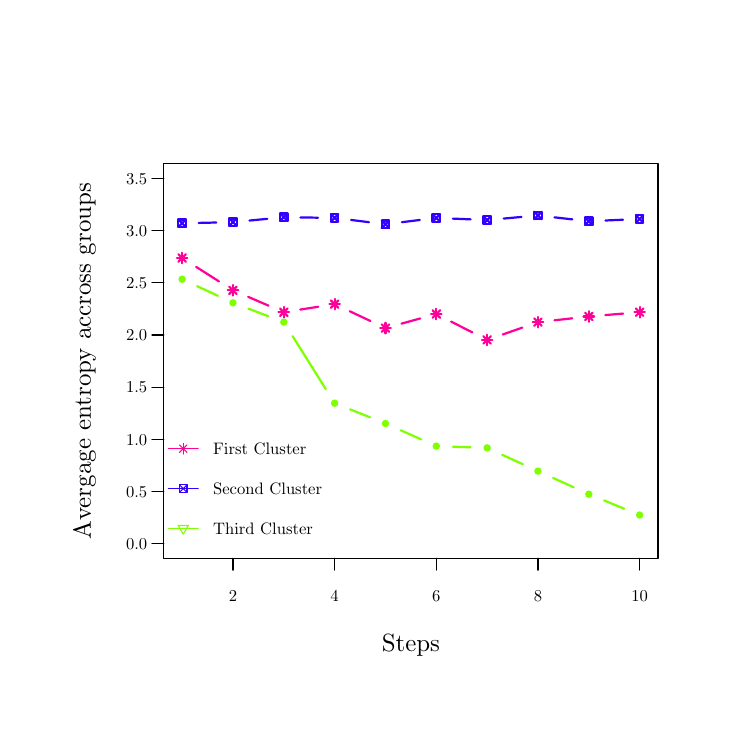
\begin{tikzpicture}[x=1pt,y=1pt]
\definecolor{fillColor}{RGB}{255,255,255}
\path[use as bounding box,fill=fillColor,fill opacity=0.00] (0,0) rectangle (252.94,252.94);
\begin{scope}
\path[clip] ( 49.20, 61.20) rectangle (227.75,203.75);
\definecolor{drawColor}{RGB}{255,0,153}

\path[draw=drawColor,line width= 0.8pt,line join=round,line cap=round] ( 60.88,166.49) -- ( 69.12,161.26);

\path[draw=drawColor,line width= 0.8pt,line join=round,line cap=round] ( 79.69,155.66) -- ( 87.04,152.49);

\path[draw=drawColor,line width= 0.8pt,line join=round,line cap=round] ( 98.48,151.06) -- (104.99,152.09);

\path[draw=drawColor,line width= 0.8pt,line join=round,line cap=round] (116.35,150.48) -- (123.86,146.94);

\path[draw=drawColor,line width= 0.8pt,line join=round,line cap=round] (135.07,145.98) -- (141.87,147.87);

\path[draw=drawColor,line width= 0.8pt,line join=round,line cap=round] (153.00,146.74) -- (160.68,142.82);

\path[draw=drawColor,line width= 0.8pt,line join=round,line cap=round] (171.69,142.08) -- (178.73,144.55);

\path[draw=drawColor,line width= 0.8pt,line join=round,line cap=round] (190.36,147.20) -- (196.80,147.92);

\path[draw=drawColor,line width= 0.8pt,line join=round,line cap=round] (208.74,149.09) -- (215.15,149.62);

\path[draw=drawColor,line width= 0.8pt,line join=round,line cap=round] ( 54.46,168.36) -- ( 57.16,171.06);

\path[draw=drawColor,line width= 0.8pt,line join=round,line cap=round] ( 54.46,171.06) -- ( 57.16,168.36);

\path[draw=drawColor,line width= 0.8pt,line join=round,line cap=round] ( 53.90,169.71) -- ( 57.72,169.71);

\path[draw=drawColor,line width= 0.8pt,line join=round,line cap=round] ( 55.81,167.80) -- ( 55.81,171.62);

\path[draw=drawColor,line width= 0.8pt,line join=round,line cap=round] ( 72.83,156.69) -- ( 75.53,159.39);

\path[draw=drawColor,line width= 0.8pt,line join=round,line cap=round] ( 72.83,159.39) -- ( 75.53,156.69);

\path[draw=drawColor,line width= 0.8pt,line join=round,line cap=round] ( 72.27,158.04) -- ( 76.09,158.04);

\path[draw=drawColor,line width= 0.8pt,line join=round,line cap=round] ( 74.18,156.13) -- ( 74.18,159.95);

\path[draw=drawColor,line width= 0.8pt,line join=round,line cap=round] ( 91.20,148.76) -- ( 93.90,151.46);

\path[draw=drawColor,line width= 0.8pt,line join=round,line cap=round] ( 91.20,151.46) -- ( 93.90,148.76);

\path[draw=drawColor,line width= 0.8pt,line join=round,line cap=round] ( 90.64,150.11) -- ( 94.46,150.11);

\path[draw=drawColor,line width= 0.8pt,line join=round,line cap=round] ( 92.55,148.20) -- ( 92.55,152.02);

\path[draw=drawColor,line width= 0.8pt,line join=round,line cap=round] (109.57,151.69) -- (112.27,154.39);

\path[draw=drawColor,line width= 0.8pt,line join=round,line cap=round] (109.57,154.39) -- (112.27,151.69);

\path[draw=drawColor,line width= 0.8pt,line join=round,line cap=round] (109.01,153.04) -- (112.83,153.04);

\path[draw=drawColor,line width= 0.8pt,line join=round,line cap=round] (110.92,151.13) -- (110.92,154.95);

\path[draw=drawColor,line width= 0.8pt,line join=round,line cap=round] (127.94,143.03) -- (130.64,145.73);

\path[draw=drawColor,line width= 0.8pt,line join=round,line cap=round] (127.94,145.73) -- (130.64,143.03);

\path[draw=drawColor,line width= 0.8pt,line join=round,line cap=round] (127.38,144.38) -- (131.20,144.38);

\path[draw=drawColor,line width= 0.8pt,line join=round,line cap=round] (129.29,142.47) -- (129.29,146.29);

\path[draw=drawColor,line width= 0.8pt,line join=round,line cap=round] (146.31,148.12) -- (149.01,150.82);

\path[draw=drawColor,line width= 0.8pt,line join=round,line cap=round] (146.31,150.82) -- (149.01,148.12);

\path[draw=drawColor,line width= 0.8pt,line join=round,line cap=round] (145.75,149.47) -- (149.57,149.47);

\path[draw=drawColor,line width= 0.8pt,line join=round,line cap=round] (147.66,147.56) -- (147.66,151.38);

\path[draw=drawColor,line width= 0.8pt,line join=round,line cap=round] (164.68,138.74) -- (167.38,141.44);

\path[draw=drawColor,line width= 0.8pt,line join=round,line cap=round] (164.68,141.44) -- (167.38,138.74);

\path[draw=drawColor,line width= 0.8pt,line join=round,line cap=round] (164.12,140.09) -- (167.93,140.09);

\path[draw=drawColor,line width= 0.8pt,line join=round,line cap=round] (166.03,138.18) -- (166.03,142.00);

\path[draw=drawColor,line width= 0.8pt,line join=round,line cap=round] (183.04,145.18) -- (185.74,147.88);

\path[draw=drawColor,line width= 0.8pt,line join=round,line cap=round] (183.04,147.88) -- (185.74,145.18);

\path[draw=drawColor,line width= 0.8pt,line join=round,line cap=round] (182.49,146.53) -- (186.30,146.53);

\path[draw=drawColor,line width= 0.8pt,line join=round,line cap=round] (184.39,144.62) -- (184.39,148.44);

\path[draw=drawColor,line width= 0.8pt,line join=round,line cap=round] (201.41,147.23) -- (204.11,149.93);

\path[draw=drawColor,line width= 0.8pt,line join=round,line cap=round] (201.41,149.93) -- (204.11,147.23);

\path[draw=drawColor,line width= 0.8pt,line join=round,line cap=round] (200.85,148.58) -- (204.67,148.58);

\path[draw=drawColor,line width= 0.8pt,line join=round,line cap=round] (202.76,146.67) -- (202.76,150.49);

\path[draw=drawColor,line width= 0.8pt,line join=round,line cap=round] (219.78,148.77) -- (222.48,151.47);

\path[draw=drawColor,line width= 0.8pt,line join=round,line cap=round] (219.78,151.47) -- (222.48,148.77);

\path[draw=drawColor,line width= 0.8pt,line join=round,line cap=round] (219.22,150.12) -- (223.04,150.12);

\path[draw=drawColor,line width= 0.8pt,line join=round,line cap=round] (221.13,148.21) -- (221.13,152.03);
\end{scope}
\begin{scope}
\path[clip] (  0.00,  0.00) rectangle (252.94,252.94);
\definecolor{drawColor}{RGB}{0,0,0}

\path[draw=drawColor,line width= 0.4pt,line join=round,line cap=round] ( 74.18, 61.20) -- (221.13, 61.20);

\path[draw=drawColor,line width= 0.4pt,line join=round,line cap=round] ( 74.18, 61.20) -- ( 74.18, 56.92);

\path[draw=drawColor,line width= 0.4pt,line join=round,line cap=round] (110.92, 61.20) -- (110.92, 56.92);

\path[draw=drawColor,line width= 0.4pt,line join=round,line cap=round] (147.66, 61.20) -- (147.66, 56.92);

\path[draw=drawColor,line width= 0.4pt,line join=round,line cap=round] (184.39, 61.20) -- (184.39, 56.92);

\path[draw=drawColor,line width= 0.4pt,line join=round,line cap=round] (221.13, 61.20) -- (221.13, 56.92);

\node[text=drawColor,anchor=base,inner sep=0pt, outer sep=0pt, scale=  0.60] at ( 74.18, 45.60) {2};

\node[text=drawColor,anchor=base,inner sep=0pt, outer sep=0pt, scale=  0.60] at (110.92, 45.60) {4};

\node[text=drawColor,anchor=base,inner sep=0pt, outer sep=0pt, scale=  0.60] at (147.66, 45.60) {6};

\node[text=drawColor,anchor=base,inner sep=0pt, outer sep=0pt, scale=  0.60] at (184.39, 45.60) {8};

\node[text=drawColor,anchor=base,inner sep=0pt, outer sep=0pt, scale=  0.60] at (221.13, 45.60) {10};

\path[draw=drawColor,line width= 0.4pt,line join=round,line cap=round] ( 49.20, 66.48) -- ( 49.20,198.47);

\path[draw=drawColor,line width= 0.4pt,line join=round,line cap=round] ( 49.20, 66.48) -- ( 44.92, 66.48);

\path[draw=drawColor,line width= 0.4pt,line join=round,line cap=round] ( 49.20, 85.33) -- ( 44.92, 85.33);

\path[draw=drawColor,line width= 0.4pt,line join=round,line cap=round] ( 49.20,104.19) -- ( 44.92,104.19);

\path[draw=drawColor,line width= 0.4pt,line join=round,line cap=round] ( 49.20,123.04) -- ( 44.92,123.04);

\path[draw=drawColor,line width= 0.4pt,line join=round,line cap=round] ( 49.20,141.90) -- ( 44.92,141.90);

\path[draw=drawColor,line width= 0.4pt,line join=round,line cap=round] ( 49.20,160.76) -- ( 44.92,160.76);

\path[draw=drawColor,line width= 0.4pt,line join=round,line cap=round] ( 49.20,179.61) -- ( 44.92,179.61);

\path[draw=drawColor,line width= 0.4pt,line join=round,line cap=round] ( 49.20,198.47) -- ( 44.92,198.47);

\node[text=drawColor,anchor=base east,inner sep=0pt, outer sep=0pt, scale=  0.60] at ( 43.20, 64.41) {0.0};

\node[text=drawColor,anchor=base east,inner sep=0pt, outer sep=0pt, scale=  0.60] at ( 43.20, 83.27) {0.5};

\node[text=drawColor,anchor=base east,inner sep=0pt, outer sep=0pt, scale=  0.60] at ( 43.20,102.12) {1.0};

\node[text=drawColor,anchor=base east,inner sep=0pt, outer sep=0pt, scale=  0.60] at ( 43.20,120.98) {1.5};

\node[text=drawColor,anchor=base east,inner sep=0pt, outer sep=0pt, scale=  0.60] at ( 43.20,139.83) {2.0};

\node[text=drawColor,anchor=base east,inner sep=0pt, outer sep=0pt, scale=  0.60] at ( 43.20,158.69) {2.5};

\node[text=drawColor,anchor=base east,inner sep=0pt, outer sep=0pt, scale=  0.60] at ( 43.20,177.54) {3.0};

\node[text=drawColor,anchor=base east,inner sep=0pt, outer sep=0pt, scale=  0.60] at ( 43.20,196.40) {3.5};

\path[draw=drawColor,line width= 0.4pt,line join=round,line cap=round] ( 49.20, 61.20) --
	(227.75, 61.20) --
	(227.75,203.75) --
	( 49.20,203.75) --
	( 49.20, 61.20);
\end{scope}
\begin{scope}
\path[clip] (  0.00,  0.00) rectangle (252.94,252.94);
\definecolor{drawColor}{RGB}{0,0,0}

\node[text=drawColor,anchor=base,inner sep=0pt, outer sep=0pt, scale=  0.90] at (138.47, 27.60) {Steps};

\node[text=drawColor,rotate= 90.00,anchor=base,inner sep=0pt, outer sep=0pt, scale=  0.90] at ( 22.80,132.47) {Avergage entropy accross groups};
\end{scope}
\begin{scope}
\path[clip] ( 49.20, 61.20) rectangle (227.75,203.75);
\definecolor{drawColor}{RGB}{51,0,255}

\path[draw=drawColor,line width= 0.8pt,line join=round,line cap=round] ( 61.81,182.39) -- ( 68.18,182.53);

\path[draw=drawColor,line width= 0.8pt,line join=round,line cap=round] ( 80.15,183.24) -- ( 86.58,183.86);

\path[draw=drawColor,line width= 0.8pt,line join=round,line cap=round] ( 98.55,184.36) -- (104.92,184.28);

\path[draw=drawColor,line width= 0.8pt,line join=round,line cap=round] (116.87,183.46) -- (123.33,182.65);

\path[draw=drawColor,line width= 0.8pt,line join=round,line cap=round] (135.24,182.65) -- (141.70,183.45);

\path[draw=drawColor,line width= 0.8pt,line join=round,line cap=round] (153.65,183.94) -- (160.03,183.67);

\path[draw=drawColor,line width= 0.8pt,line join=round,line cap=round] (172.00,183.96) -- (178.42,184.54);

\path[draw=drawColor,line width= 0.8pt,line join=round,line cap=round] (190.36,184.40) -- (196.80,183.67);

\path[draw=drawColor,line width= 0.8pt,line join=round,line cap=round] (208.76,183.26) -- (215.14,183.54);

\path[draw=drawColor,line width= 0.8pt,line join=round,line cap=round] ( 54.46,180.91) rectangle ( 57.16,183.61);

\path[draw=drawColor,line width= 0.8pt,line join=round,line cap=round] ( 54.46,180.91) -- ( 57.16,183.61);

\path[draw=drawColor,line width= 0.8pt,line join=round,line cap=round] ( 54.46,183.61) -- ( 57.16,180.91);

\path[draw=drawColor,line width= 0.8pt,line join=round,line cap=round] ( 72.83,181.32) rectangle ( 75.53,184.02);

\path[draw=drawColor,line width= 0.8pt,line join=round,line cap=round] ( 72.83,181.32) -- ( 75.53,184.02);

\path[draw=drawColor,line width= 0.8pt,line join=round,line cap=round] ( 72.83,184.02) -- ( 75.53,181.32);

\path[draw=drawColor,line width= 0.8pt,line join=round,line cap=round] ( 91.20,183.09) rectangle ( 93.90,185.79);

\path[draw=drawColor,line width= 0.8pt,line join=round,line cap=round] ( 91.20,183.09) -- ( 93.90,185.79);

\path[draw=drawColor,line width= 0.8pt,line join=round,line cap=round] ( 91.20,185.79) -- ( 93.90,183.09);

\path[draw=drawColor,line width= 0.8pt,line join=round,line cap=round] (109.57,182.85) rectangle (112.27,185.55);

\path[draw=drawColor,line width= 0.8pt,line join=round,line cap=round] (109.57,182.85) -- (112.27,185.55);

\path[draw=drawColor,line width= 0.8pt,line join=round,line cap=round] (109.57,185.55) -- (112.27,182.85);

\path[draw=drawColor,line width= 0.8pt,line join=round,line cap=round] (127.94,180.56) rectangle (130.64,183.26);

\path[draw=drawColor,line width= 0.8pt,line join=round,line cap=round] (127.94,180.56) -- (130.64,183.26);

\path[draw=drawColor,line width= 0.8pt,line join=round,line cap=round] (127.94,183.26) -- (130.64,180.56);

\path[draw=drawColor,line width= 0.8pt,line join=round,line cap=round] (146.31,182.84) rectangle (149.01,185.54);

\path[draw=drawColor,line width= 0.8pt,line join=round,line cap=round] (146.31,182.84) -- (149.01,185.54);

\path[draw=drawColor,line width= 0.8pt,line join=round,line cap=round] (146.31,185.54) -- (149.01,182.84);

\path[draw=drawColor,line width= 0.8pt,line join=round,line cap=round] (164.68,182.07) rectangle (167.38,184.77);

\path[draw=drawColor,line width= 0.8pt,line join=round,line cap=round] (164.68,182.07) -- (167.38,184.77);

\path[draw=drawColor,line width= 0.8pt,line join=round,line cap=round] (164.68,184.77) -- (167.38,182.07);

\path[draw=drawColor,line width= 0.8pt,line join=round,line cap=round] (183.04,183.72) rectangle (185.74,186.42);

\path[draw=drawColor,line width= 0.8pt,line join=round,line cap=round] (183.04,183.72) -- (185.74,186.42);

\path[draw=drawColor,line width= 0.8pt,line join=round,line cap=round] (183.04,186.42) -- (185.74,183.72);

\path[draw=drawColor,line width= 0.8pt,line join=round,line cap=round] (201.41,181.64) rectangle (204.11,184.34);

\path[draw=drawColor,line width= 0.8pt,line join=round,line cap=round] (201.41,181.64) -- (204.11,184.34);

\path[draw=drawColor,line width= 0.8pt,line join=round,line cap=round] (201.41,184.34) -- (204.11,181.64);

\path[draw=drawColor,line width= 0.8pt,line join=round,line cap=round] (219.78,182.46) rectangle (222.48,185.16);

\path[draw=drawColor,line width= 0.8pt,line join=round,line cap=round] (219.78,182.46) -- (222.48,185.16);

\path[draw=drawColor,line width= 0.8pt,line join=round,line cap=round] (219.78,185.16) -- (222.48,182.46);
\definecolor{drawColor}{RGB}{128,255,0}

\path[draw=drawColor,line width= 0.8pt,line join=round,line cap=round] ( 61.26,159.52) -- ( 68.74,156.05);

\path[draw=drawColor,line width= 0.8pt,line join=round,line cap=round] ( 79.79,151.39) -- ( 86.94,148.68);

\path[draw=drawColor,line width= 0.8pt,line join=round,line cap=round] ( 95.74,141.46) -- (107.73,122.33);

\path[draw=drawColor,line width= 0.8pt,line join=round,line cap=round] (116.49,115.02) -- (123.72,112.14);

\path[draw=drawColor,line width= 0.8pt,line join=round,line cap=round] (134.77,107.47) -- (142.18,104.17);

\path[draw=drawColor,line width= 0.8pt,line join=round,line cap=round] (153.65,101.52) -- (160.03,101.30);

\path[draw=drawColor,line width= 0.8pt,line join=round,line cap=round] (171.48, 98.59) -- (178.94, 95.19);

\path[draw=drawColor,line width= 0.8pt,line join=round,line cap=round] (189.86, 90.22) -- (197.30, 86.85);

\path[draw=drawColor,line width= 0.8pt,line join=round,line cap=round] (208.31, 82.09) -- (215.58, 79.11);
\definecolor{fillColor}{RGB}{128,255,0}

\path[fill=fillColor] ( 55.81,162.04) circle (  1.35);

\path[fill=fillColor] ( 74.18,153.52) circle (  1.35);

\path[fill=fillColor] ( 92.55,146.54) circle (  1.35);

\path[fill=fillColor] (110.92,117.25) circle (  1.35);

\path[fill=fillColor] (129.29,109.91) circle (  1.35);

\path[fill=fillColor] (147.66,101.73) circle (  1.35);

\path[fill=fillColor] (166.03,101.09) circle (  1.35);

\path[fill=fillColor] (184.39, 92.70) circle (  1.35);

\path[fill=fillColor] (202.76, 84.37) circle (  1.35);

\path[fill=fillColor] (221.13, 76.84) circle (  1.35);
\definecolor{drawColor}{RGB}{255,0,153}

\path[draw=drawColor,line width= 0.4pt,line join=round,line cap=round] ( 50.82,100.80) -- ( 61.62,100.80);
\definecolor{drawColor}{RGB}{51,0,255}

\path[draw=drawColor,line width= 0.4pt,line join=round,line cap=round] ( 50.82, 86.40) -- ( 61.62, 86.40);
\definecolor{drawColor}{RGB}{128,255,0}

\path[draw=drawColor,line width= 0.4pt,line join=round,line cap=round] ( 50.82, 72.00) -- ( 61.62, 72.00);
\definecolor{drawColor}{RGB}{255,0,153}

\path[draw=drawColor,line width= 0.4pt,line join=round,line cap=round] ( 54.87, 99.45) -- ( 57.57,102.15);

\path[draw=drawColor,line width= 0.4pt,line join=round,line cap=round] ( 54.87,102.15) -- ( 57.57, 99.45);

\path[draw=drawColor,line width= 0.4pt,line join=round,line cap=round] ( 54.31,100.80) -- ( 58.13,100.80);

\path[draw=drawColor,line width= 0.4pt,line join=round,line cap=round] ( 56.22, 98.89) -- ( 56.22,102.71);
\definecolor{drawColor}{RGB}{51,0,255}

\path[draw=drawColor,line width= 0.4pt,line join=round,line cap=round] ( 54.87, 85.05) rectangle ( 57.57, 87.75);

\path[draw=drawColor,line width= 0.4pt,line join=round,line cap=round] ( 54.87, 85.05) -- ( 57.57, 87.75);

\path[draw=drawColor,line width= 0.4pt,line join=round,line cap=round] ( 54.87, 87.75) -- ( 57.57, 85.05);
\definecolor{drawColor}{RGB}{128,255,0}

\path[draw=drawColor,line width= 0.4pt,line join=round,line cap=round] ( 56.22, 69.90) --
	( 58.04, 73.05) --
	( 54.40, 73.05) --
	( 56.22, 69.90);
\definecolor{drawColor}{RGB}{0,0,0}

\node[text=drawColor,anchor=base west,inner sep=0pt, outer sep=0pt, scale=  0.60] at ( 67.02, 98.73) {First Cluster};

\node[text=drawColor,anchor=base west,inner sep=0pt, outer sep=0pt, scale=  0.60] at ( 67.02, 84.33) {Second Cluster};

\node[text=drawColor,anchor=base west,inner sep=0pt, outer sep=0pt, scale=  0.60] at ( 67.02, 69.93) {Third Cluster};
\end{scope}
\end{tikzpicture}
 & % Created by tikzDevice version 0.10.1 on 2016-06-30 12:41:21
% !TEX encoding = UTF-8 Unicode
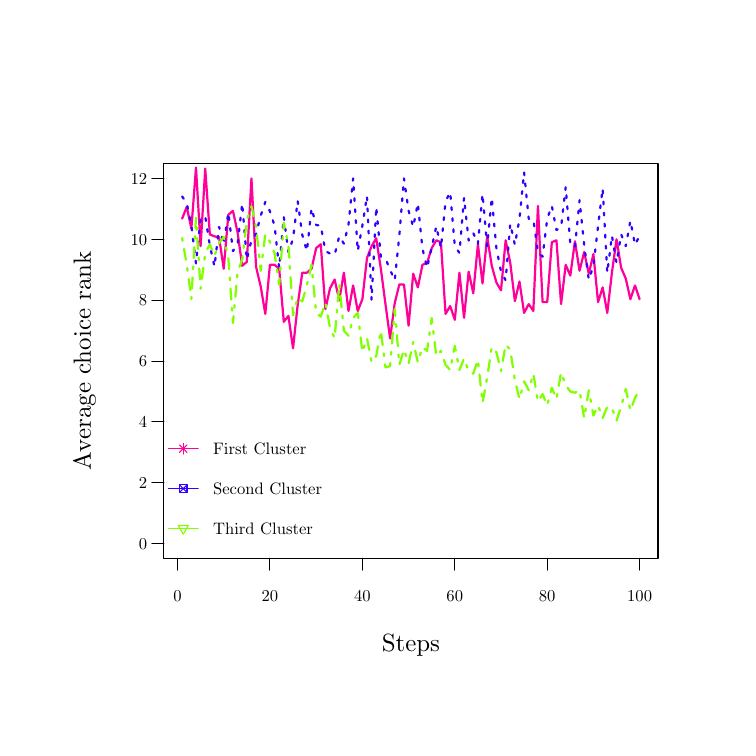
\begin{tikzpicture}[x=1pt,y=1pt]
\definecolor{fillColor}{RGB}{255,255,255}
\path[use as bounding box,fill=fillColor,fill opacity=0.00] (0,0) rectangle (252.94,252.94);
\begin{scope}
\path[clip] ( 49.20, 61.20) rectangle (227.75,203.75);
\definecolor{drawColor}{RGB}{255,0,153}

\path[draw=drawColor,line width= 0.8pt,line join=round,line cap=round] ( 55.81,183.92) --
	( 57.48,188.18) --
	( 59.15,180.37) --
	( 60.82,202.37) --
	( 62.49,173.98) --
	( 64.16,202.01) --
	( 65.83,178.24) --
	( 67.50,177.53) --
	( 69.17,177.18) --
	( 70.84,165.82) --
	( 72.51,185.34) --
	( 74.18,186.76) --
	( 75.85,178.95) --
	( 77.52,166.89) --
	( 79.19,168.31) --
	( 80.86,198.47) --
	( 82.53,166.53) --
	( 84.20,159.44) --
	( 85.87,149.50) --
	( 87.54,167.24) --
	( 89.21,167.24) --
	( 90.88,165.82) --
	( 92.55,146.66) --
	( 94.22,148.79) --
	( 95.89,137.08) --
	( 97.56,152.70) --
	( 99.23,164.40) --
	(100.90,164.40) --
	(102.57,165.82) --
	(104.24,173.27) --
	(105.91,174.69) --
	(107.58,151.28) --
	(109.25,158.73) --
	(110.92,161.92) --
	(112.59,154.47) --
	(114.26,164.40) --
	(115.93,150.57) --
	(117.60,159.79) --
	(119.27,150.57) --
	(120.94,154.82) --
	(122.61,169.73) --
	(124.28,173.98) --
	(125.95,176.82) --
	(127.62,165.82) --
	(129.29,153.05) --
	(130.96,140.63) --
	(132.63,153.41) --
	(134.30,160.15) --
	(135.97,160.15) --
	(137.64,145.25) --
	(139.31,164.05) --
	(140.98,159.08) --
	(142.65,167.24) --
	(144.32,167.95) --
	(145.99,173.27) --
	(147.66,176.11) --
	(149.33,175.40) --
	(151.00,149.50) --
	(152.67,152.34) --
	(154.34,147.37) --
	(156.01,164.40) --
	(157.68,148.08) --
	(159.35,164.76) --
	(161.02,156.95) --
	(162.69,174.69) --
	(164.36,160.50) --
	(166.03,177.53) --
	(167.70,166.89) --
	(169.37,160.86) --
	(171.04,158.02) --
	(172.71,176.11) --
	(174.38,167.95) --
	(176.05,154.12) --
	(177.71,161.21) --
	(179.38,149.86) --
	(181.05,153.05) --
	(182.72,150.57) --
	(184.39,188.53) --
	(186.06,153.76) --
	(187.73,153.76) --
	(189.40,175.40) --
	(191.07,176.11) --
	(192.74,153.05) --
	(194.41,167.24) --
	(196.08,163.34) --
	(197.75,175.76) --
	(199.42,165.11) --
	(201.09,171.86) --
	(202.76,164.05) --
	(204.43,171.15) --
	(206.10,153.76) --
	(207.77,159.08) --
	(209.44,149.86) --
	(211.11,164.40) --
	(212.78,176.47) --
	(214.45,166.18) --
	(216.12,162.28) --
	(217.79,154.82) --
	(219.46,159.79) --
	(221.13,154.82);
\end{scope}
\begin{scope}
\path[clip] (  0.00,  0.00) rectangle (252.94,252.94);
\definecolor{drawColor}{RGB}{0,0,0}

\path[draw=drawColor,line width= 0.4pt,line join=round,line cap=round] ( 54.14, 61.20) -- (221.13, 61.20);

\path[draw=drawColor,line width= 0.4pt,line join=round,line cap=round] ( 54.14, 61.20) -- ( 54.14, 56.92);

\path[draw=drawColor,line width= 0.4pt,line join=round,line cap=round] ( 87.54, 61.20) -- ( 87.54, 56.92);

\path[draw=drawColor,line width= 0.4pt,line join=round,line cap=round] (120.94, 61.20) -- (120.94, 56.92);

\path[draw=drawColor,line width= 0.4pt,line join=round,line cap=round] (154.34, 61.20) -- (154.34, 56.92);

\path[draw=drawColor,line width= 0.4pt,line join=round,line cap=round] (187.73, 61.20) -- (187.73, 56.92);

\path[draw=drawColor,line width= 0.4pt,line join=round,line cap=round] (221.13, 61.20) -- (221.13, 56.92);

\node[text=drawColor,anchor=base,inner sep=0pt, outer sep=0pt, scale=  0.60] at ( 54.14, 45.60) {0};

\node[text=drawColor,anchor=base,inner sep=0pt, outer sep=0pt, scale=  0.60] at ( 87.54, 45.60) {20};

\node[text=drawColor,anchor=base,inner sep=0pt, outer sep=0pt, scale=  0.60] at (120.94, 45.60) {40};

\node[text=drawColor,anchor=base,inner sep=0pt, outer sep=0pt, scale=  0.60] at (154.34, 45.60) {60};

\node[text=drawColor,anchor=base,inner sep=0pt, outer sep=0pt, scale=  0.60] at (187.73, 45.60) {80};

\node[text=drawColor,anchor=base,inner sep=0pt, outer sep=0pt, scale=  0.60] at (221.13, 45.60) {100};

\path[draw=drawColor,line width= 0.4pt,line join=round,line cap=round] ( 49.20, 66.48) -- ( 49.20,198.47);

\path[draw=drawColor,line width= 0.4pt,line join=round,line cap=round] ( 49.20, 66.48) -- ( 44.92, 66.48);

\path[draw=drawColor,line width= 0.4pt,line join=round,line cap=round] ( 49.20, 88.48) -- ( 44.92, 88.48);

\path[draw=drawColor,line width= 0.4pt,line join=round,line cap=round] ( 49.20,110.47) -- ( 44.92,110.47);

\path[draw=drawColor,line width= 0.4pt,line join=round,line cap=round] ( 49.20,132.47) -- ( 44.92,132.47);

\path[draw=drawColor,line width= 0.4pt,line join=round,line cap=round] ( 49.20,154.47) -- ( 44.92,154.47);

\path[draw=drawColor,line width= 0.4pt,line join=round,line cap=round] ( 49.20,176.47) -- ( 44.92,176.47);

\path[draw=drawColor,line width= 0.4pt,line join=round,line cap=round] ( 49.20,198.47) -- ( 44.92,198.47);

\node[text=drawColor,anchor=base east,inner sep=0pt, outer sep=0pt, scale=  0.60] at ( 43.20, 64.41) {0};

\node[text=drawColor,anchor=base east,inner sep=0pt, outer sep=0pt, scale=  0.60] at ( 43.20, 86.41) {2};

\node[text=drawColor,anchor=base east,inner sep=0pt, outer sep=0pt, scale=  0.60] at ( 43.20,108.41) {4};

\node[text=drawColor,anchor=base east,inner sep=0pt, outer sep=0pt, scale=  0.60] at ( 43.20,130.41) {6};

\node[text=drawColor,anchor=base east,inner sep=0pt, outer sep=0pt, scale=  0.60] at ( 43.20,152.40) {8};

\node[text=drawColor,anchor=base east,inner sep=0pt, outer sep=0pt, scale=  0.60] at ( 43.20,174.40) {10};

\node[text=drawColor,anchor=base east,inner sep=0pt, outer sep=0pt, scale=  0.60] at ( 43.20,196.40) {12};

\path[draw=drawColor,line width= 0.4pt,line join=round,line cap=round] ( 49.20, 61.20) --
	(227.75, 61.20) --
	(227.75,203.75) --
	( 49.20,203.75) --
	( 49.20, 61.20);
\end{scope}
\begin{scope}
\path[clip] (  0.00,  0.00) rectangle (252.94,252.94);
\definecolor{drawColor}{RGB}{0,0,0}

\node[text=drawColor,anchor=base,inner sep=0pt, outer sep=0pt, scale=  0.90] at (138.47, 27.60) {Steps};

\node[text=drawColor,rotate= 90.00,anchor=base,inner sep=0pt, outer sep=0pt, scale=  0.90] at ( 22.80,132.47) {Average choice rank};
\end{scope}
\begin{scope}
\path[clip] ( 49.20, 61.20) rectangle (227.75,203.75);
\definecolor{drawColor}{RGB}{51,0,255}

\path[draw=drawColor,line width= 0.8pt,dash pattern=on 1pt off 3pt ,line join=round,line cap=round] ( 55.81,191.96) --
	( 57.48,189.49) --
	( 59.15,181.41) --
	( 60.82,167.71) --
	( 62.49,184.10) --
	( 64.16,184.77) --
	( 65.83,174.22) --
	( 67.50,166.59) --
	( 69.17,180.96) --
	( 70.84,174.67) --
	( 72.51,186.12) --
	( 74.18,172.20) --
	( 75.85,174.67) --
	( 77.52,189.49) --
	( 79.19,169.06) --
	( 80.86,176.24) --
	( 82.53,178.49) --
	( 84.20,185.00) --
	( 85.87,189.94) --
	( 87.54,186.57) --
	( 89.21,181.41) --
	( 90.88,166.14) --
	( 92.55,184.55) --
	( 94.22,171.75) --
	( 95.89,176.69) --
	( 97.56,190.38) --
	( 99.23,178.04) --
	(100.90,172.20) --
	(102.57,187.69) --
	(104.24,181.63) --
	(105.91,181.41) --
	(107.58,172.20) --
	(109.25,171.31) --
	(110.92,170.86) --
	(112.59,177.59) --
	(114.26,174.90) --
	(115.93,181.86) --
	(117.60,198.47) --
	(119.27,172.20) --
	(120.94,181.41) --
	(122.61,192.18) --
	(124.28,154.47) --
	(125.95,188.14) --
	(127.62,170.18) --
	(129.29,169.51) --
	(130.96,165.47) --
	(132.63,161.65) --
	(134.30,177.81) --
	(135.97,198.47) --
	(137.64,186.79) --
	(139.31,180.96) --
	(140.98,189.49) --
	(142.65,173.10) --
	(144.32,166.14) --
	(145.99,173.55) --
	(147.66,181.18) --
	(149.33,173.33) --
	(151.00,190.16) --
	(152.67,193.53) --
	(154.34,174.00) --
	(156.01,171.53) --
	(157.68,191.51) --
	(159.35,176.02) --
	(161.02,178.71) --
	(162.69,174.90) --
	(164.36,192.85) --
	(166.03,174.00) --
	(167.70,191.51) --
	(169.37,173.33) --
	(171.04,164.80) --
	(172.71,161.65) --
	(174.38,182.08) --
	(176.05,174.45) --
	(177.71,183.88) --
	(179.38,200.71) --
	(181.05,183.88) --
	(182.72,183.65) --
	(184.39,171.98) --
	(186.06,170.18) --
	(187.73,183.88) --
	(189.40,188.59) --
	(191.07,179.83) --
	(192.74,180.73) --
	(194.41,195.32) --
	(196.08,174.90) --
	(197.75,173.55) --
	(199.42,190.61) --
	(201.09,174.45) --
	(202.76,161.88) --
	(204.43,166.82) --
	(206.10,181.18) --
	(207.77,194.87) --
	(209.44,164.35) --
	(211.11,177.81) --
	(212.78,167.94) --
	(214.45,178.26) --
	(216.12,174.00) --
	(217.79,183.20) --
	(219.46,174.45) --
	(221.13,177.81);
\definecolor{drawColor}{RGB}{128,255,0}

\path[draw=drawColor,line width= 0.8pt,dash pattern=on 1pt off 3pt on 4pt off 3pt ,line join=round,line cap=round] ( 55.81,176.93) --
	( 57.48,167.30) --
	( 59.15,154.93) --
	( 60.82,184.26) --
	( 62.49,158.59) --
	( 64.16,171.43) --
	( 65.83,174.63) --
	( 67.50,170.51) --
	( 69.17,175.09) --
	( 70.84,177.38) --
	( 72.51,169.59) --
	( 74.18,146.22) --
	( 75.85,164.55) --
	( 77.52,169.14) --
	( 79.19,183.34) --
	( 80.86,188.38) --
	( 82.53,181.05) --
	( 84.20,165.01) --
	( 85.87,178.30) --
	( 87.54,175.55) --
	( 89.21,171.43) --
	( 90.88,159.97) --
	( 92.55,182.43) --
	( 94.22,174.18) --
	( 95.89,148.97) --
	( 97.56,155.39) --
	( 99.23,154.01) --
	(100.90,159.97) --
	(102.57,167.30) --
	(104.24,149.89) --
	(105.91,148.51) --
	(107.58,153.55) --
	(109.25,144.39) --
	(110.92,140.72) --
	(112.59,160.43) --
	(114.26,143.47) --
	(115.93,141.64) --
	(117.60,148.05) --
	(119.27,149.89) --
	(120.94,135.68) --
	(122.61,140.72) --
	(124.28,132.01) --
	(125.95,134.31) --
	(127.62,143.47) --
	(129.29,130.18) --
	(130.96,130.64) --
	(132.63,151.26) --
	(134.30,131.10) --
	(135.97,136.60) --
	(137.64,131.56) --
	(139.31,139.35) --
	(140.98,132.01) --
	(142.65,137.51) --
	(144.32,136.14) --
	(145.99,148.05) --
	(147.66,134.31) --
	(149.33,136.14) --
	(151.00,131.10) --
	(152.67,129.26) --
	(154.34,137.97) --
	(156.01,129.26) --
	(157.68,133.39) --
	(159.35,128.81) --
	(161.02,127.89) --
	(162.69,132.93) --
	(164.36,117.35) --
	(166.03,126.51) --
	(167.70,137.51) --
	(169.37,135.68) --
	(171.04,128.81) --
	(172.71,138.43) --
	(174.38,136.60) --
	(176.05,125.60) --
	(177.71,118.72) --
	(179.38,125.14) --
	(181.05,121.93) --
	(182.72,127.89) --
	(184.39,117.81) --
	(186.06,120.56) --
	(187.73,116.43) --
	(189.40,122.85) --
	(191.07,118.72) --
	(192.74,128.35) --
	(194.41,123.77) --
	(196.08,121.47) --
	(197.75,121.02) --
	(199.42,121.93) --
	(201.09,111.85) --
	(202.76,121.93) --
	(204.43,112.77) --
	(206.10,116.43) --
	(207.77,111.85) --
	(209.44,115.97) --
	(211.11,115.52) --
	(212.78,110.93) --
	(214.45,115.97) --
	(216.12,122.39) --
	(217.79,114.60) --
	(219.46,119.18) --
	(221.13,121.93);
\definecolor{drawColor}{RGB}{255,0,153}

\path[draw=drawColor,line width= 0.4pt,line join=round,line cap=round] ( 50.82,100.80) -- ( 61.62,100.80);
\definecolor{drawColor}{RGB}{51,0,255}

\path[draw=drawColor,line width= 0.4pt,line join=round,line cap=round] ( 50.82, 86.40) -- ( 61.62, 86.40);
\definecolor{drawColor}{RGB}{128,255,0}

\path[draw=drawColor,line width= 0.4pt,line join=round,line cap=round] ( 50.82, 72.00) -- ( 61.62, 72.00);
\definecolor{drawColor}{RGB}{255,0,153}

\path[draw=drawColor,line width= 0.4pt,line join=round,line cap=round] ( 54.87, 99.45) -- ( 57.57,102.15);

\path[draw=drawColor,line width= 0.4pt,line join=round,line cap=round] ( 54.87,102.15) -- ( 57.57, 99.45);

\path[draw=drawColor,line width= 0.4pt,line join=round,line cap=round] ( 54.31,100.80) -- ( 58.13,100.80);

\path[draw=drawColor,line width= 0.4pt,line join=round,line cap=round] ( 56.22, 98.89) -- ( 56.22,102.71);
\definecolor{drawColor}{RGB}{51,0,255}

\path[draw=drawColor,line width= 0.4pt,line join=round,line cap=round] ( 54.87, 85.05) rectangle ( 57.57, 87.75);

\path[draw=drawColor,line width= 0.4pt,line join=round,line cap=round] ( 54.87, 85.05) -- ( 57.57, 87.75);

\path[draw=drawColor,line width= 0.4pt,line join=round,line cap=round] ( 54.87, 87.75) -- ( 57.57, 85.05);
\definecolor{drawColor}{RGB}{128,255,0}

\path[draw=drawColor,line width= 0.4pt,line join=round,line cap=round] ( 56.22, 69.90) --
	( 58.04, 73.05) --
	( 54.40, 73.05) --
	( 56.22, 69.90);
\definecolor{drawColor}{RGB}{0,0,0}

\node[text=drawColor,anchor=base west,inner sep=0pt, outer sep=0pt, scale=  0.60] at ( 67.02, 98.73) {First Cluster};

\node[text=drawColor,anchor=base west,inner sep=0pt, outer sep=0pt, scale=  0.60] at ( 67.02, 84.33) {Second Cluster};

\node[text=drawColor,anchor=base west,inner sep=0pt, outer sep=0pt, scale=  0.60] at ( 67.02, 69.93) {Third Cluster};
\end{scope}
\end{tikzpicture}
 \\
		(\textbf{a}) Blockwise entropy by cluster & (\textbf{b}) Average choice rank by cluster 
	\end{tabular} \quad
	\caption{Clustering on choices vs. model parameter estimation (top sub figures: experiment 1, high noise, bottom: experiment 1, low noise)}
	\label{fig:cluse1c4}
\end{figure}


\subsection{Prison data}

We were provided with experimental data from \cite{Yechiam2008}. Again we try to apply our methods to cluster different groups in the data. The participants had to perform a modified version of the Iowa gambling task, where reward structure of the decks are changing over time.\\
In particular we have data of 96 individuals with different criminal profile. Within this data we don't have a control group. Given that participants performed a different version of the test we could add a control data from publicly available data sets (see \cite{Steingroever2015}).\\
Table \ref{tab:tabps} gives a broad summary of some demographics of the participants. The samples for each groups are not balanced. 

\begin{table}[H]
	\scriptsize
	 \centering 
	 		\caption{Summary prison data (means with standard deviation in parenthesis)} 
	\resizebox{\textwidth}{!}{\begin{tabular}{ llrcccc} 
		\toprule 
		\textbf{ID} & \textbf{Criminal profile} & \textbf{Count} & \textbf{Age} & \textbf{TABE Score} & \textbf{Education} & \textbf{Beta IQ} \\ 
		\hline
	1&Theft/Burglary & $22$ & $25.36$  (7.03) & $11.09$ (1.29) & $7.38$ (3.34 )& $92.91$ (14.37) \\ 
	2&Robbery & $6$ & $24.17$ (9.83) & $11.00$ (0.63) & $9.22$ (3.30) & $96.50$ (7.58) \\          
	3&Sex & $17$ & $33.41$ (13.59) & $10.97$ (1.47) & $9.15$ (2.98) & $99.65$ (11.74) \\       
	4&Drug & $22$ & $30.91$ (10.11)  & $11.64$ (1.85)& $9.06$   (2.70)  & $100.36$ (12.92) \\     
	5&OWI & $4$ & $38.75$ (7.27) & $10.88$ (1.93) & $7.12$ (1.17)& $94.25$ (10.40) \\        
	6&Assault & $10$ & $27.20$ (8.77) & $12.30$ (2.41)& $7.62$ (2.28) & $94.50$ (11.29) \\       
	7&Escape/ Failure To Appear & $4$ & $2.008$ (5.60)& $11.00$ (1.35)& $7.78$  (3.21)& $96.50$  (14.18)\\     
	8&Vandalism & $1$ & $18.00$ (NA)& $11.00$ (NA)& $9.40$ (NA)& $90.00$ (NA)\\ 
	9&Forgery & $7$ & $34.57$ (13.14)& $10.93$ (5.15) & $9.83$ (3.82)& $100.71$ (11.01)\\       
	10&Probabiton & $1$ & $38.00$ (NA)& $12.00$ (NA)& $6.30$ (NA)& $92.00$ (NA)\\ 
	11 &Other & $2$ & $35.00$ (9.90)& $11.50$ (0.00)& $9.20$ (4.67)& $95.00$ (5.66)\\       
		\bottomrule 
	\end{tabular} }
		\label{tab:tabps} 
\end{table} 

In figure \ref{fig:ent} we show display some of the behavioural data. Given the number of participants we averaged the by criminal profile to see if we can find differences in across groups. We excluded "OWI", "escape", "vandalism", "probation" and "others" from this figures since the number of observations is fairly small. This also gives a more clear insight in the data.\\
Figure \ref{fig:ent} (a) and (b) show the blockwise ratio of disadvantageous choices and the development of cumulative disadvantageous choices. A clear separation can not be observed from those plots. From figure (b) we can at most see a slight decreasing trend for forgery, sex robbery and theft, while drug and stay slightly higher.\footnote{\cite{stout2004} found a constant disadvantageous behaviour for cocaine abusers (see next section)}\\
Figure \ref{fig:ent} (d) shows the average cumulative entropy averaged across groups. We observe a random behaviour independent from group affiliation. Notably, people with assault/murder profile are show constantly the highest value. We can observe the same from the blockwise entropy from figure (c) we could observe the same behaviour.

{\renewcommand{\arraystretch}{0.4}%
\begin{figure}[H]
	\centering
	\small
	\hspace*{-0.7in}
	\begin{tabular}{cc}
	% Created by tikzDevice version 0.10.1 on 2016-06-29 15:59:44
% !TEX encoding = UTF-8 Unicode
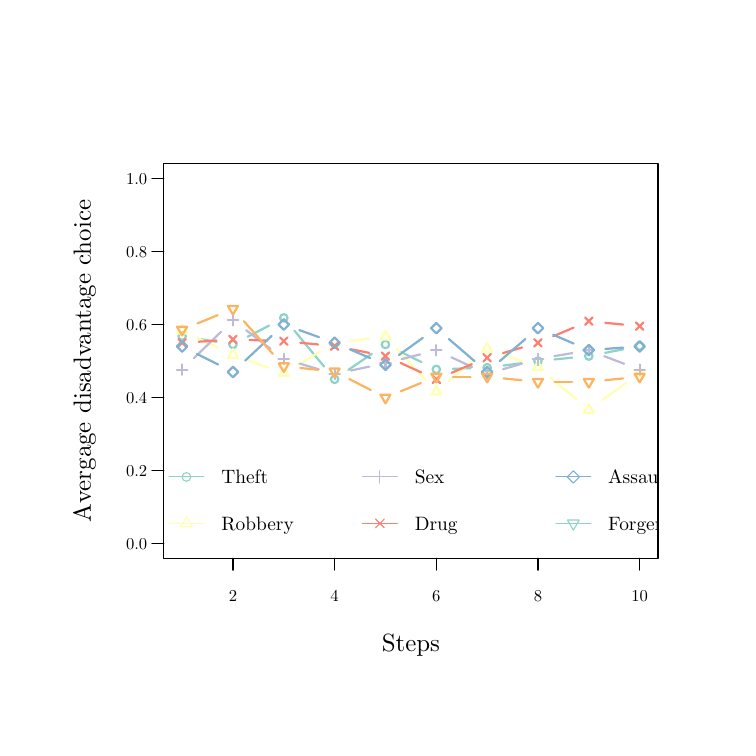
\begin{tikzpicture}[x=1pt,y=1pt]
\definecolor{fillColor}{RGB}{255,255,255}
\path[use as bounding box,fill=fillColor,fill opacity=0.00] (0,0) rectangle (252.94,252.94);
\begin{scope}
\path[clip] ( 49.20, 61.20) rectangle (227.75,203.75);
\definecolor{drawColor}{RGB}{141,211,199}

\path[draw=drawColor,line width= 0.8pt,line join=round,line cap=round] ( 61.73,140.50) -- ( 68.26,139.44);

\path[draw=drawColor,line width= 0.8pt,line join=round,line cap=round] ( 79.50,141.25) -- ( 87.23,145.29);

\path[draw=drawColor,line width= 0.8pt,line join=round,line cap=round] ( 96.38,143.45) -- (107.09,130.50);

\path[draw=drawColor,line width= 0.8pt,line join=round,line cap=round] (115.87,129.27) -- (124.34,135.08);

\path[draw=drawColor,line width= 0.8pt,line join=round,line cap=round] (134.68,135.83) -- (142.27,132.11);

\path[draw=drawColor,line width= 0.8pt,line join=round,line cap=round] (153.65,129.67) -- (160.03,129.88);

\path[draw=drawColor,line width= 0.8pt,line join=round,line cap=round] (171.98,130.85) -- (178.45,131.70);

\path[draw=drawColor,line width= 0.8pt,line join=round,line cap=round] (190.37,133.06) -- (196.79,133.69);

\path[draw=drawColor,line width= 0.8pt,line join=round,line cap=round] (208.65,135.43) -- (215.24,136.72);

\path[draw=drawColor,line width= 0.8pt,line join=round,line cap=round] ( 55.81,141.47) circle (  1.35);

\path[draw=drawColor,line width= 0.8pt,line join=round,line cap=round] ( 74.18,138.47) circle (  1.35);

\path[draw=drawColor,line width= 0.8pt,line join=round,line cap=round] ( 92.55,148.07) circle (  1.35);

\path[draw=drawColor,line width= 0.8pt,line join=round,line cap=round] (110.92,125.87) circle (  1.35);

\path[draw=drawColor,line width= 0.8pt,line join=round,line cap=round] (129.29,138.47) circle (  1.35);

\path[draw=drawColor,line width= 0.8pt,line join=round,line cap=round] (147.66,129.47) circle (  1.35);

\path[draw=drawColor,line width= 0.8pt,line join=round,line cap=round] (166.03,130.07) circle (  1.35);

\path[draw=drawColor,line width= 0.8pt,line join=round,line cap=round] (184.39,132.47) circle (  1.35);

\path[draw=drawColor,line width= 0.8pt,line join=round,line cap=round] (202.76,134.27) circle (  1.35);

\path[draw=drawColor,line width= 0.8pt,line join=round,line cap=round] (221.13,137.87) circle (  1.35);
\end{scope}
\begin{scope}
\path[clip] (  0.00,  0.00) rectangle (252.94,252.94);
\definecolor{drawColor}{RGB}{0,0,0}

\path[draw=drawColor,line width= 0.4pt,line join=round,line cap=round] ( 74.18, 61.20) -- (221.13, 61.20);

\path[draw=drawColor,line width= 0.4pt,line join=round,line cap=round] ( 74.18, 61.20) -- ( 74.18, 56.92);

\path[draw=drawColor,line width= 0.4pt,line join=round,line cap=round] (110.92, 61.20) -- (110.92, 56.92);

\path[draw=drawColor,line width= 0.4pt,line join=round,line cap=round] (147.66, 61.20) -- (147.66, 56.92);

\path[draw=drawColor,line width= 0.4pt,line join=round,line cap=round] (184.39, 61.20) -- (184.39, 56.92);

\path[draw=drawColor,line width= 0.4pt,line join=round,line cap=round] (221.13, 61.20) -- (221.13, 56.92);

\node[text=drawColor,anchor=base,inner sep=0pt, outer sep=0pt, scale=  0.60] at ( 74.18, 45.60) {2};

\node[text=drawColor,anchor=base,inner sep=0pt, outer sep=0pt, scale=  0.60] at (110.92, 45.60) {4};

\node[text=drawColor,anchor=base,inner sep=0pt, outer sep=0pt, scale=  0.60] at (147.66, 45.60) {6};

\node[text=drawColor,anchor=base,inner sep=0pt, outer sep=0pt, scale=  0.60] at (184.39, 45.60) {8};

\node[text=drawColor,anchor=base,inner sep=0pt, outer sep=0pt, scale=  0.60] at (221.13, 45.60) {10};

\path[draw=drawColor,line width= 0.4pt,line join=round,line cap=round] ( 49.20, 66.48) -- ( 49.20,198.47);

\path[draw=drawColor,line width= 0.4pt,line join=round,line cap=round] ( 49.20, 66.48) -- ( 44.92, 66.48);

\path[draw=drawColor,line width= 0.4pt,line join=round,line cap=round] ( 49.20, 92.88) -- ( 44.92, 92.88);

\path[draw=drawColor,line width= 0.4pt,line join=round,line cap=round] ( 49.20,119.27) -- ( 44.92,119.27);

\path[draw=drawColor,line width= 0.4pt,line join=round,line cap=round] ( 49.20,145.67) -- ( 44.92,145.67);

\path[draw=drawColor,line width= 0.4pt,line join=round,line cap=round] ( 49.20,172.07) -- ( 44.92,172.07);

\path[draw=drawColor,line width= 0.4pt,line join=round,line cap=round] ( 49.20,198.47) -- ( 44.92,198.47);

\node[text=drawColor,anchor=base east,inner sep=0pt, outer sep=0pt, scale=  0.60] at ( 43.20, 64.41) {0.0};

\node[text=drawColor,anchor=base east,inner sep=0pt, outer sep=0pt, scale=  0.60] at ( 43.20, 90.81) {0.2};

\node[text=drawColor,anchor=base east,inner sep=0pt, outer sep=0pt, scale=  0.60] at ( 43.20,117.21) {0.4};

\node[text=drawColor,anchor=base east,inner sep=0pt, outer sep=0pt, scale=  0.60] at ( 43.20,143.60) {0.6};

\node[text=drawColor,anchor=base east,inner sep=0pt, outer sep=0pt, scale=  0.60] at ( 43.20,170.00) {0.8};

\node[text=drawColor,anchor=base east,inner sep=0pt, outer sep=0pt, scale=  0.60] at ( 43.20,196.40) {1.0};

\path[draw=drawColor,line width= 0.4pt,line join=round,line cap=round] ( 49.20, 61.20) --
	(227.75, 61.20) --
	(227.75,203.75) --
	( 49.20,203.75) --
	( 49.20, 61.20);
\end{scope}
\begin{scope}
\path[clip] (  0.00,  0.00) rectangle (252.94,252.94);
\definecolor{drawColor}{RGB}{0,0,0}

\node[text=drawColor,anchor=base,inner sep=0pt, outer sep=0pt, scale=  0.90] at (138.47, 27.60) {Steps};

\node[text=drawColor,rotate= 90.00,anchor=base,inner sep=0pt, outer sep=0pt, scale=  0.90] at ( 22.80,132.47) {Avergage disadvantage choice};
\end{scope}
\begin{scope}
\path[clip] ( 49.20, 61.20) rectangle (227.75,203.75);
\definecolor{drawColor}{RGB}{255,255,179}

\path[draw=drawColor,line width= 0.8pt,line join=round,line cap=round] ( 61.22,140.88) -- ( 68.77,137.26);

\path[draw=drawColor,line width= 0.8pt,line join=round,line cap=round] ( 79.83,132.64) -- ( 86.90,130.10);

\path[draw=drawColor,line width= 0.8pt,line join=round,line cap=round] ( 97.70,131.16) -- (105.77,135.99);

\path[draw=drawColor,line width= 0.8pt,line join=round,line cap=round] (116.88,139.79) -- (123.33,140.56);

\path[draw=drawColor,line width= 0.8pt,line join=round,line cap=round] (133.37,136.87) -- (143.58,125.87);

\path[draw=drawColor,line width= 0.8pt,line join=round,line cap=round] (152.26,125.33) -- (161.43,133.02);

\path[draw=drawColor,line width= 0.8pt,line join=round,line cap=round] (171.67,134.84) -- (178.75,132.30);

\path[draw=drawColor,line width= 0.8pt,line join=round,line cap=round] (188.99,126.42) -- (198.17,118.73);

\path[draw=drawColor,line width= 0.8pt,line join=round,line cap=round] (207.64,118.38) -- (216.26,124.57);

\path[draw=drawColor,line width= 0.8pt,line join=round,line cap=round] ( 55.81,145.57) --
	( 57.63,142.42) --
	( 53.99,142.42) --
	( 55.81,145.57);

\path[draw=drawColor,line width= 0.8pt,line join=round,line cap=round] ( 74.18,136.77) --
	( 76.00,133.62) --
	( 72.36,133.62) --
	( 74.18,136.77);

\path[draw=drawColor,line width= 0.8pt,line join=round,line cap=round] ( 92.55,130.17) --
	( 94.37,127.02) --
	( 90.73,127.02) --
	( 92.55,130.17);

\path[draw=drawColor,line width= 0.8pt,line join=round,line cap=round] (110.92,141.17) --
	(112.74,138.02) --
	(109.10,138.02) --
	(110.92,141.17);

\path[draw=drawColor,line width= 0.8pt,line join=round,line cap=round] (129.29,143.37) --
	(131.11,140.22) --
	(127.47,140.22) --
	(129.29,143.37);

\path[draw=drawColor,line width= 0.8pt,line join=round,line cap=round] (147.66,123.57) --
	(149.48,120.42) --
	(145.84,120.42) --
	(147.66,123.57);

\path[draw=drawColor,line width= 0.8pt,line join=round,line cap=round] (166.03,138.97) --
	(167.84,135.82) --
	(164.21,135.82) --
	(166.03,138.97);

\path[draw=drawColor,line width= 0.8pt,line join=round,line cap=round] (184.39,132.37) --
	(186.21,129.22) --
	(182.58,129.22) --
	(184.39,132.37);

\path[draw=drawColor,line width= 0.8pt,line join=round,line cap=round] (202.76,116.97) --
	(204.58,113.82) --
	(200.95,113.82) --
	(202.76,116.97);

\path[draw=drawColor,line width= 0.8pt,line join=round,line cap=round] (221.13,130.17) --
	(222.95,127.02) --
	(219.31,127.02) --
	(221.13,130.17);
\definecolor{drawColor}{RGB}{190,186,218}

\path[draw=drawColor,line width= 0.8pt,line join=round,line cap=round] ( 60.11,133.55) -- ( 69.88,143.04);

\path[draw=drawColor,line width= 0.8pt,line join=round,line cap=round] ( 78.96,143.59) -- ( 87.78,136.88);

\path[draw=drawColor,line width= 0.8pt,line join=round,line cap=round] ( 98.30,131.55) -- (105.17,129.52);

\path[draw=drawColor,line width= 0.8pt,line join=round,line cap=round] (116.79,129.05) -- (123.42,130.46);

\path[draw=drawColor,line width= 0.8pt,line join=round,line cap=round] (135.10,133.17) -- (141.84,134.88);

\path[draw=drawColor,line width= 0.8pt,line join=round,line cap=round] (153.10,133.82) -- (160.59,130.34);

\path[draw=drawColor,line width= 0.8pt,line join=round,line cap=round] (171.78,129.52) -- (178.64,131.55);

\path[draw=drawColor,line width= 0.8pt,line join=round,line cap=round] (190.31,134.25) -- (196.85,135.35);

\path[draw=drawColor,line width= 0.8pt,line join=round,line cap=round] (208.37,134.22) -- (215.52,131.50);

\path[draw=drawColor,line width= 0.8pt,line join=round,line cap=round] ( 53.90,129.37) -- ( 57.72,129.37);

\path[draw=drawColor,line width= 0.8pt,line join=round,line cap=round] ( 55.81,127.46) -- ( 55.81,131.28);

\path[draw=drawColor,line width= 0.8pt,line join=round,line cap=round] ( 72.27,147.22) -- ( 76.09,147.22);

\path[draw=drawColor,line width= 0.8pt,line join=round,line cap=round] ( 74.18,145.31) -- ( 74.18,149.13);

\path[draw=drawColor,line width= 0.8pt,line join=round,line cap=round] ( 90.64,133.25) -- ( 94.46,133.25);

\path[draw=drawColor,line width= 0.8pt,line join=round,line cap=round] ( 92.55,131.34) -- ( 92.55,135.16);

\path[draw=drawColor,line width= 0.8pt,line join=round,line cap=round] (109.01,127.81) -- (112.83,127.81);

\path[draw=drawColor,line width= 0.8pt,line join=round,line cap=round] (110.92,125.90) -- (110.92,129.72);

\path[draw=drawColor,line width= 0.8pt,line join=round,line cap=round] (127.38,131.70) -- (131.20,131.70);

\path[draw=drawColor,line width= 0.8pt,line join=round,line cap=round] (129.29,129.79) -- (129.29,133.61);

\path[draw=drawColor,line width= 0.8pt,line join=round,line cap=round] (145.75,136.35) -- (149.57,136.35);

\path[draw=drawColor,line width= 0.8pt,line join=round,line cap=round] (147.66,134.45) -- (147.66,138.26);

\path[draw=drawColor,line width= 0.8pt,line join=round,line cap=round] (164.12,127.81) -- (167.93,127.81);

\path[draw=drawColor,line width= 0.8pt,line join=round,line cap=round] (166.03,125.90) -- (166.03,129.72);

\path[draw=drawColor,line width= 0.8pt,line join=round,line cap=round] (182.49,133.25) -- (186.30,133.25);

\path[draw=drawColor,line width= 0.8pt,line join=round,line cap=round] (184.39,131.34) -- (184.39,135.16);

\path[draw=drawColor,line width= 0.8pt,line join=round,line cap=round] (200.85,136.35) -- (204.67,136.35);

\path[draw=drawColor,line width= 0.8pt,line join=round,line cap=round] (202.76,134.45) -- (202.76,138.26);

\path[draw=drawColor,line width= 0.8pt,line join=round,line cap=round] (219.22,129.37) -- (223.04,129.37);

\path[draw=drawColor,line width= 0.8pt,line join=round,line cap=round] (221.13,127.46) -- (221.13,131.28);
\definecolor{drawColor}{RGB}{251,128,114}

\path[draw=drawColor,line width= 0.8pt,line join=round,line cap=round] ( 61.80,139.46) -- ( 68.19,139.88);

\path[draw=drawColor,line width= 0.8pt,line join=round,line cap=round] ( 80.18,140.08) -- ( 86.55,139.87);

\path[draw=drawColor,line width= 0.8pt,line join=round,line cap=round] ( 98.52,139.09) -- (104.95,138.46);

\path[draw=drawColor,line width= 0.8pt,line join=round,line cap=round] (116.81,136.72) -- (123.40,135.43);

\path[draw=drawColor,line width= 0.8pt,line join=round,line cap=round] (134.74,131.78) -- (142.20,128.37);

\path[draw=drawColor,line width= 0.8pt,line join=round,line cap=round] (153.18,128.22) -- (160.50,131.33);

\path[draw=drawColor,line width= 0.8pt,line join=round,line cap=round] (171.78,135.36) -- (178.64,137.38);

\path[draw=drawColor,line width= 0.8pt,line join=round,line cap=round] (189.92,141.42) -- (197.24,144.53);

\path[draw=drawColor,line width= 0.8pt,line join=round,line cap=round] (208.73,146.29) -- (215.16,145.66);

\path[draw=drawColor,line width= 0.8pt,line join=round,line cap=round] ( 54.46,137.72) -- ( 57.16,140.42);

\path[draw=drawColor,line width= 0.8pt,line join=round,line cap=round] ( 54.46,140.42) -- ( 57.16,137.72);

\path[draw=drawColor,line width= 0.8pt,line join=round,line cap=round] ( 72.83,138.92) -- ( 75.53,141.62);

\path[draw=drawColor,line width= 0.8pt,line join=round,line cap=round] ( 72.83,141.62) -- ( 75.53,138.92);

\path[draw=drawColor,line width= 0.8pt,line join=round,line cap=round] ( 91.20,138.32) -- ( 93.90,141.02);

\path[draw=drawColor,line width= 0.8pt,line join=round,line cap=round] ( 91.20,141.02) -- ( 93.90,138.32);

\path[draw=drawColor,line width= 0.8pt,line join=round,line cap=round] (109.57,136.52) -- (112.27,139.22);

\path[draw=drawColor,line width= 0.8pt,line join=round,line cap=round] (109.57,139.22) -- (112.27,136.52);

\path[draw=drawColor,line width= 0.8pt,line join=round,line cap=round] (127.94,132.92) -- (130.64,135.62);

\path[draw=drawColor,line width= 0.8pt,line join=round,line cap=round] (127.94,135.62) -- (130.64,132.92);

\path[draw=drawColor,line width= 0.8pt,line join=round,line cap=round] (146.31,124.52) -- (149.01,127.22);

\path[draw=drawColor,line width= 0.8pt,line join=round,line cap=round] (146.31,127.22) -- (149.01,124.52);

\path[draw=drawColor,line width= 0.8pt,line join=round,line cap=round] (164.68,132.32) -- (167.38,135.02);

\path[draw=drawColor,line width= 0.8pt,line join=round,line cap=round] (164.68,135.02) -- (167.38,132.32);

\path[draw=drawColor,line width= 0.8pt,line join=round,line cap=round] (183.04,137.72) -- (185.74,140.42);

\path[draw=drawColor,line width= 0.8pt,line join=round,line cap=round] (183.04,140.42) -- (185.74,137.72);

\path[draw=drawColor,line width= 0.8pt,line join=round,line cap=round] (201.41,145.52) -- (204.11,148.22);

\path[draw=drawColor,line width= 0.8pt,line join=round,line cap=round] (201.41,148.22) -- (204.11,145.52);

\path[draw=drawColor,line width= 0.8pt,line join=round,line cap=round] (219.78,143.72) -- (222.48,146.42);

\path[draw=drawColor,line width= 0.8pt,line join=round,line cap=round] (219.78,146.42) -- (222.48,143.72);
\definecolor{drawColor}{RGB}{128,177,211}

\path[draw=drawColor,line width= 0.8pt,line join=round,line cap=round] ( 61.17,135.06) -- ( 68.82,131.21);

\path[draw=drawColor,line width= 0.8pt,line join=round,line cap=round] ( 78.57,132.61) -- ( 88.17,141.58);

\path[draw=drawColor,line width= 0.8pt,line join=round,line cap=round] ( 98.20,143.64) -- (105.27,141.10);

\path[draw=drawColor,line width= 0.8pt,line join=round,line cap=round] (116.43,136.70) -- (123.78,133.53);

\path[draw=drawColor,line width= 0.8pt,line join=round,line cap=round] (134.16,134.65) -- (142.78,140.85);

\path[draw=drawColor,line width= 0.8pt,line join=round,line cap=round] (152.20,140.43) -- (161.48,132.43);

\path[draw=drawColor,line width= 0.8pt,line join=round,line cap=round] (170.57,132.43) -- (179.85,140.43);

\path[draw=drawColor,line width= 0.8pt,line join=round,line cap=round] (189.90,141.98) -- (197.25,138.81);

\path[draw=drawColor,line width= 0.8pt,line join=round,line cap=round] (208.75,136.86) -- (215.15,137.32);

\path[draw=drawColor,line width= 0.8pt,line join=round,line cap=round] ( 53.90,137.75) --
	( 55.81,139.66) --
	( 57.72,137.75) --
	( 55.81,135.84) --
	( 53.90,137.75);

\path[draw=drawColor,line width= 0.8pt,line join=round,line cap=round] ( 72.27,128.51) --
	( 74.18,130.42) --
	( 76.09,128.51) --
	( 74.18,126.60) --
	( 72.27,128.51);

\path[draw=drawColor,line width= 0.8pt,line join=round,line cap=round] ( 90.64,145.67) --
	( 92.55,147.58) --
	( 94.46,145.67) --
	( 92.55,143.76) --
	( 90.64,145.67);

\path[draw=drawColor,line width= 0.8pt,line join=round,line cap=round] (109.01,139.07) --
	(110.92,140.98) --
	(112.83,139.07) --
	(110.92,137.16) --
	(109.01,139.07);

\path[draw=drawColor,line width= 0.8pt,line join=round,line cap=round] (127.38,131.15) --
	(129.29,133.06) --
	(131.20,131.15) --
	(129.29,129.24) --
	(127.38,131.15);

\path[draw=drawColor,line width= 0.8pt,line join=round,line cap=round] (145.75,144.35) --
	(147.66,146.26) --
	(149.57,144.35) --
	(147.66,142.44) --
	(145.75,144.35);

\path[draw=drawColor,line width= 0.8pt,line join=round,line cap=round] (164.12,128.51) --
	(166.03,130.42) --
	(167.93,128.51) --
	(166.03,126.60) --
	(164.12,128.51);

\path[draw=drawColor,line width= 0.8pt,line join=round,line cap=round] (182.49,144.35) --
	(184.39,146.26) --
	(186.30,144.35) --
	(184.39,142.44) --
	(182.49,144.35);

\path[draw=drawColor,line width= 0.8pt,line join=round,line cap=round] (200.85,136.43) --
	(202.76,138.34) --
	(204.67,136.43) --
	(202.76,134.52) --
	(200.85,136.43);

\path[draw=drawColor,line width= 0.8pt,line join=round,line cap=round] (219.22,137.75) --
	(221.13,139.66) --
	(223.04,137.75) --
	(221.13,135.84) --
	(219.22,137.75);
\definecolor{drawColor}{RGB}{253,180,98}

\path[draw=drawColor,line width= 0.8pt,line join=round,line cap=round] ( 61.36,146.06) -- ( 68.63,149.05);

\path[draw=drawColor,line width= 0.8pt,line join=round,line cap=round] ( 78.16,146.84) -- ( 88.57,135.08);

\path[draw=drawColor,line width= 0.8pt,line join=round,line cap=round] ( 98.52,129.97) -- (104.95,129.31);

\path[draw=drawColor,line width= 0.8pt,line join=round,line cap=round] (116.26,125.96) -- (123.95,122.01);

\path[draw=drawColor,line width= 0.8pt,line join=round,line cap=round] (134.84,121.55) -- (142.11,124.54);

\path[draw=drawColor,line width= 0.8pt,line join=round,line cap=round] (153.66,126.82) -- (160.03,126.82);

\path[draw=drawColor,line width= 0.8pt,line join=round,line cap=round] (171.99,126.20) -- (178.43,125.54);

\path[draw=drawColor,line width= 0.8pt,line join=round,line cap=round] (190.39,124.93) -- (196.76,124.93);

\path[draw=drawColor,line width= 0.8pt,line join=round,line cap=round] (208.73,125.54) -- (215.16,126.20);

\path[draw=drawColor,line width= 0.8pt,line join=round,line cap=round] ( 55.81,141.69) --
	( 57.63,144.84) --
	( 53.99,144.84) --
	( 55.81,141.69);

\path[draw=drawColor,line width= 0.8pt,line join=round,line cap=round] ( 74.18,149.23) --
	( 76.00,152.38) --
	( 72.36,152.38) --
	( 74.18,149.23);

\path[draw=drawColor,line width= 0.8pt,line join=round,line cap=round] ( 92.55,128.49) --
	( 94.37,131.64) --
	( 90.73,131.64) --
	( 92.55,128.49);

\path[draw=drawColor,line width= 0.8pt,line join=round,line cap=round] (110.92,126.60) --
	(112.74,129.75) --
	(109.10,129.75) --
	(110.92,126.60);

\path[draw=drawColor,line width= 0.8pt,line join=round,line cap=round] (129.29,117.17) --
	(131.11,120.32) --
	(127.47,120.32) --
	(129.29,117.17);

\path[draw=drawColor,line width= 0.8pt,line join=round,line cap=round] (147.66,124.72) --
	(149.48,127.87) --
	(145.84,127.87) --
	(147.66,124.72);

\path[draw=drawColor,line width= 0.8pt,line join=round,line cap=round] (166.03,124.72) --
	(167.84,127.87) --
	(164.21,127.87) --
	(166.03,124.72);

\path[draw=drawColor,line width= 0.8pt,line join=round,line cap=round] (184.39,122.83) --
	(186.21,125.98) --
	(182.58,125.98) --
	(184.39,122.83);

\path[draw=drawColor,line width= 0.8pt,line join=round,line cap=round] (202.76,122.83) --
	(204.58,125.98) --
	(200.95,125.98) --
	(202.76,122.83);

\path[draw=drawColor,line width= 0.8pt,line join=round,line cap=round] (221.13,124.72) --
	(222.95,127.87) --
	(219.31,127.87) --
	(221.13,124.72);
\definecolor{drawColor}{RGB}{141,211,199}

\path[draw=drawColor,line width= 0.4pt,line join=round,line cap=round] ( 51.09, 90.60) -- ( 63.69, 90.60);
\definecolor{drawColor}{RGB}{255,255,179}

\path[draw=drawColor,line width= 0.4pt,line join=round,line cap=round] ( 51.09, 73.80) -- ( 63.69, 73.80);
\definecolor{drawColor}{RGB}{190,186,218}

\path[draw=drawColor,line width= 0.4pt,line join=round,line cap=round] (120.98, 90.60) -- (133.58, 90.60);
\definecolor{drawColor}{RGB}{251,128,114}

\path[draw=drawColor,line width= 0.4pt,line join=round,line cap=round] (120.98, 73.80) -- (133.58, 73.80);
\definecolor{drawColor}{RGB}{128,177,211}

\path[draw=drawColor,line width= 0.4pt,line join=round,line cap=round] (190.88, 90.60) -- (203.48, 90.60);
\definecolor{drawColor}{RGB}{141,211,199}

\path[draw=drawColor,line width= 0.4pt,line join=round,line cap=round] (190.88, 73.80) -- (203.48, 73.80);

\path[draw=drawColor,line width= 0.4pt,line join=round,line cap=round] ( 57.39, 90.60) circle (  1.57);
\definecolor{drawColor}{RGB}{255,255,179}

\path[draw=drawColor,line width= 0.4pt,line join=round,line cap=round] ( 57.39, 76.25) --
	( 59.51, 72.58) --
	( 55.27, 72.58) --
	( 57.39, 76.25);
\definecolor{drawColor}{RGB}{190,186,218}

\path[draw=drawColor,line width= 0.4pt,line join=round,line cap=round] (125.06, 90.60) -- (129.51, 90.60);

\path[draw=drawColor,line width= 0.4pt,line join=round,line cap=round] (127.28, 88.37) -- (127.28, 92.83);
\definecolor{drawColor}{RGB}{251,128,114}

\path[draw=drawColor,line width= 0.4pt,line join=round,line cap=round] (125.71, 72.22) -- (128.86, 75.38);

\path[draw=drawColor,line width= 0.4pt,line join=round,line cap=round] (125.71, 75.38) -- (128.86, 72.22);
\definecolor{drawColor}{RGB}{128,177,211}

\path[draw=drawColor,line width= 0.4pt,line join=round,line cap=round] (194.95, 90.60) --
	(197.18, 92.83) --
	(199.41, 90.60) --
	(197.18, 88.37) --
	(194.95, 90.60);
\definecolor{drawColor}{RGB}{141,211,199}

\path[draw=drawColor,line width= 0.4pt,line join=round,line cap=round] (197.18, 71.35) --
	(199.30, 75.02) --
	(195.06, 75.02) --
	(197.18, 71.35);
\definecolor{drawColor}{RGB}{0,0,0}

\node[text=drawColor,anchor=base west,inner sep=0pt, outer sep=0pt, scale=  0.70] at ( 69.99, 88.19) {Theft};

\node[text=drawColor,anchor=base west,inner sep=0pt, outer sep=0pt, scale=  0.70] at ( 69.99, 71.39) {Robbery};

\node[text=drawColor,anchor=base west,inner sep=0pt, outer sep=0pt, scale=  0.70] at (139.88, 88.19) {Sex};

\node[text=drawColor,anchor=base west,inner sep=0pt, outer sep=0pt, scale=  0.70] at (139.88, 71.39) {Drug};

\node[text=drawColor,anchor=base west,inner sep=0pt, outer sep=0pt, scale=  0.70] at (209.78, 88.19) {Assault/Murder};

\node[text=drawColor,anchor=base west,inner sep=0pt, outer sep=0pt, scale=  0.70] at (209.78, 71.39) {Forgery};
\end{scope}
\end{tikzpicture}
 & % Created by tikzDevice version 0.10.1 on 2016-06-29 16:07:49
% !TEX encoding = UTF-8 Unicode
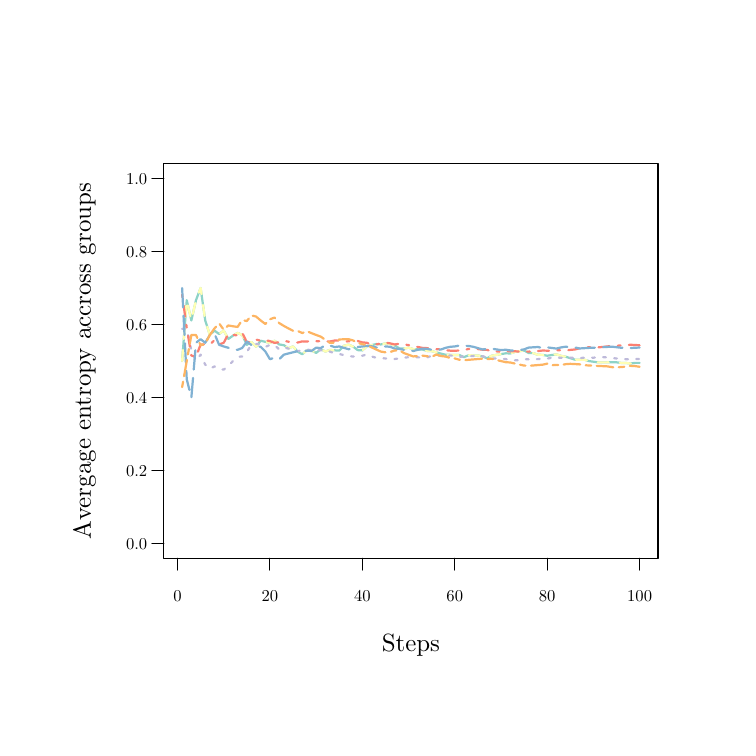
\begin{tikzpicture}[x=1pt,y=1pt]
\definecolor{fillColor}{RGB}{255,255,255}
\path[use as bounding box,fill=fillColor,fill opacity=0.00] (0,0) rectangle (252.94,252.94);
\begin{scope}
\path[clip] ( 49.20, 61.20) rectangle (227.75,203.75);
\definecolor{drawColor}{RGB}{141,211,199}

\path[draw=drawColor,line width= 0.8pt,line join=round,line cap=round] ( 55.81,132.47) --
	( 57.48,154.47) --
	( 59.15,147.14) --
	( 60.82,154.47) --
	( 62.49,158.87) --
	( 64.16,147.14) --
	( 65.83,141.90) --
	( 67.50,143.47) --
	( 69.17,142.25) --
	( 70.84,143.47) --
	( 72.51,140.47) --
	( 74.18,141.64) --
	( 75.85,142.63) --
	( 77.52,141.90) --
	( 79.19,138.34) --
	( 80.86,139.35) --
	( 82.53,137.65) --
	( 84.20,139.81) --
	( 85.87,139.42) --
	( 87.54,139.07) --
	( 89.21,139.81) --
	( 90.88,138.47) --
	( 92.55,138.21) --
	( 94.22,137.06) --
	( 95.89,137.75) --
	( 97.56,135.86) --
	( 99.23,134.92) --
	(100.90,136.40) --
	(102.57,136.27) --
	(104.24,135.41) --
	(105.91,136.73) --
	(107.58,135.91) --
	(109.25,136.47) --
	(110.92,136.35) --
	(112.59,136.24) --
	(114.26,137.97) --
	(115.93,138.42) --
	(117.60,137.68) --
	(119.27,136.42) --
	(120.94,136.32) --
	(122.61,137.84) --
	(124.28,138.23) --
	(125.95,138.61) --
	(127.62,138.47) --
	(129.29,138.83) --
	(130.96,138.69) --
	(132.63,138.09) --
	(134.30,137.06) --
	(135.97,136.96) --
	(137.64,137.31) --
	(139.31,136.79) --
	(140.98,136.70) --
	(142.65,136.62) --
	(144.32,136.14) --
	(145.99,136.07) --
	(147.66,135.62) --
	(149.33,135.17) --
	(151.00,134.75) --
	(152.67,134.71) --
	(154.34,134.67) --
	(156.01,134.64) --
	(157.68,133.89) --
	(159.35,134.57) --
	(161.02,134.53) --
	(162.69,134.50) --
	(164.36,134.14) --
	(166.03,133.46) --
	(167.70,134.41) --
	(169.37,134.70) --
	(171.04,134.99) --
	(172.71,135.26) --
	(174.38,135.22) --
	(176.05,135.79) --
	(177.71,136.04) --
	(179.38,136.29) --
	(181.05,135.37) --
	(182.72,135.33) --
	(184.39,134.73) --
	(186.06,134.70) --
	(187.73,134.40) --
	(189.40,134.65) --
	(191.07,134.89) --
	(192.74,134.33) --
	(194.41,134.04) --
	(196.08,133.51) --
	(197.75,132.98) --
	(199.42,132.98) --
	(201.09,132.97) --
	(202.76,132.47) --
	(204.43,132.23) --
	(206.10,131.99) --
	(207.77,131.99) --
	(209.44,132.00) --
	(211.11,132.00) --
	(212.78,132.01) --
	(214.45,131.79) --
	(216.12,131.79) --
	(217.79,131.57) --
	(219.46,131.81) --
	(221.13,131.81);
\end{scope}
\begin{scope}
\path[clip] (  0.00,  0.00) rectangle (252.94,252.94);
\definecolor{drawColor}{RGB}{0,0,0}

\path[draw=drawColor,line width= 0.4pt,line join=round,line cap=round] ( 54.14, 61.20) -- (221.13, 61.20);

\path[draw=drawColor,line width= 0.4pt,line join=round,line cap=round] ( 54.14, 61.20) -- ( 54.14, 56.92);

\path[draw=drawColor,line width= 0.4pt,line join=round,line cap=round] ( 87.54, 61.20) -- ( 87.54, 56.92);

\path[draw=drawColor,line width= 0.4pt,line join=round,line cap=round] (120.94, 61.20) -- (120.94, 56.92);

\path[draw=drawColor,line width= 0.4pt,line join=round,line cap=round] (154.34, 61.20) -- (154.34, 56.92);

\path[draw=drawColor,line width= 0.4pt,line join=round,line cap=round] (187.73, 61.20) -- (187.73, 56.92);

\path[draw=drawColor,line width= 0.4pt,line join=round,line cap=round] (221.13, 61.20) -- (221.13, 56.92);

\node[text=drawColor,anchor=base,inner sep=0pt, outer sep=0pt, scale=  0.60] at ( 54.14, 45.60) {0};

\node[text=drawColor,anchor=base,inner sep=0pt, outer sep=0pt, scale=  0.60] at ( 87.54, 45.60) {20};

\node[text=drawColor,anchor=base,inner sep=0pt, outer sep=0pt, scale=  0.60] at (120.94, 45.60) {40};

\node[text=drawColor,anchor=base,inner sep=0pt, outer sep=0pt, scale=  0.60] at (154.34, 45.60) {60};

\node[text=drawColor,anchor=base,inner sep=0pt, outer sep=0pt, scale=  0.60] at (187.73, 45.60) {80};

\node[text=drawColor,anchor=base,inner sep=0pt, outer sep=0pt, scale=  0.60] at (221.13, 45.60) {100};

\path[draw=drawColor,line width= 0.4pt,line join=round,line cap=round] ( 49.20, 66.48) -- ( 49.20,198.47);

\path[draw=drawColor,line width= 0.4pt,line join=round,line cap=round] ( 49.20, 66.48) -- ( 44.92, 66.48);

\path[draw=drawColor,line width= 0.4pt,line join=round,line cap=round] ( 49.20, 92.88) -- ( 44.92, 92.88);

\path[draw=drawColor,line width= 0.4pt,line join=round,line cap=round] ( 49.20,119.27) -- ( 44.92,119.27);

\path[draw=drawColor,line width= 0.4pt,line join=round,line cap=round] ( 49.20,145.67) -- ( 44.92,145.67);

\path[draw=drawColor,line width= 0.4pt,line join=round,line cap=round] ( 49.20,172.07) -- ( 44.92,172.07);

\path[draw=drawColor,line width= 0.4pt,line join=round,line cap=round] ( 49.20,198.47) -- ( 44.92,198.47);

\node[text=drawColor,anchor=base east,inner sep=0pt, outer sep=0pt, scale=  0.60] at ( 43.20, 64.41) {0.0};

\node[text=drawColor,anchor=base east,inner sep=0pt, outer sep=0pt, scale=  0.60] at ( 43.20, 90.81) {0.2};

\node[text=drawColor,anchor=base east,inner sep=0pt, outer sep=0pt, scale=  0.60] at ( 43.20,117.21) {0.4};

\node[text=drawColor,anchor=base east,inner sep=0pt, outer sep=0pt, scale=  0.60] at ( 43.20,143.60) {0.6};

\node[text=drawColor,anchor=base east,inner sep=0pt, outer sep=0pt, scale=  0.60] at ( 43.20,170.00) {0.8};

\node[text=drawColor,anchor=base east,inner sep=0pt, outer sep=0pt, scale=  0.60] at ( 43.20,196.40) {1.0};

\path[draw=drawColor,line width= 0.4pt,line join=round,line cap=round] ( 49.20, 61.20) --
	(227.75, 61.20) --
	(227.75,203.75) --
	( 49.20,203.75) --
	( 49.20, 61.20);
\end{scope}
\begin{scope}
\path[clip] (  0.00,  0.00) rectangle (252.94,252.94);
\definecolor{drawColor}{RGB}{0,0,0}

\node[text=drawColor,anchor=base,inner sep=0pt, outer sep=0pt, scale=  0.90] at (138.47, 27.60) {Steps};

\node[text=drawColor,rotate= 90.00,anchor=base,inner sep=0pt, outer sep=0pt, scale=  0.90] at ( 22.80,132.47) {Avergage entropy accross groups};
\end{scope}
\begin{scope}
\path[clip] ( 49.20, 61.20) rectangle (227.75,203.75);
\definecolor{drawColor}{RGB}{255,255,179}

\path[draw=drawColor,line width= 0.8pt,dash pattern=on 4pt off 4pt ,line join=round,line cap=round] ( 55.81,132.47) --
	( 57.48,154.47) --
	( 59.15,147.14) --
	( 60.82,154.47) --
	( 62.49,158.87) --
	( 64.16,147.14) --
	( 65.83,141.90) --
	( 67.50,143.47) --
	( 69.17,142.25) --
	( 70.84,143.47) --
	( 72.51,140.47) --
	( 74.18,141.64) --
	( 75.85,142.63) --
	( 77.52,141.90) --
	( 79.19,138.34) --
	( 80.86,139.35) --
	( 82.53,137.65) --
	( 84.20,139.81) --
	( 85.87,139.42) --
	( 87.54,139.07) --
	( 89.21,139.81) --
	( 90.88,138.47) --
	( 92.55,138.21) --
	( 94.22,137.06) --
	( 95.89,137.75) --
	( 97.56,135.86) --
	( 99.23,134.92) --
	(100.90,136.40) --
	(102.57,136.27) --
	(104.24,135.41) --
	(105.91,136.73) --
	(107.58,135.91) --
	(109.25,136.47) --
	(110.92,136.35) --
	(112.59,136.24) --
	(114.26,137.97) --
	(115.93,138.42) --
	(117.60,137.68) --
	(119.27,136.42) --
	(120.94,136.32) --
	(122.61,137.84) --
	(124.28,138.23) --
	(125.95,138.61) --
	(127.62,138.47) --
	(129.29,138.83) --
	(130.96,138.69) --
	(132.63,138.09) --
	(134.30,137.06) --
	(135.97,136.96) --
	(137.64,137.31) --
	(139.31,136.79) --
	(140.98,136.70) --
	(142.65,136.62) --
	(144.32,136.14) --
	(145.99,136.07) --
	(147.66,135.62) --
	(149.33,135.17) --
	(151.00,134.75) --
	(152.67,134.71) --
	(154.34,134.67) --
	(156.01,134.64) --
	(157.68,133.89) --
	(159.35,134.57) --
	(161.02,134.53) --
	(162.69,134.50) --
	(164.36,134.14) --
	(166.03,133.46) --
	(167.70,134.41) --
	(169.37,134.70) --
	(171.04,134.99) --
	(172.71,135.26) --
	(174.38,135.22) --
	(176.05,135.79) --
	(177.71,136.04) --
	(179.38,136.29) --
	(181.05,135.37) --
	(182.72,135.33) --
	(184.39,134.73) --
	(186.06,134.70) --
	(187.73,134.40) --
	(189.40,134.65) --
	(191.07,134.89) --
	(192.74,134.33) --
	(194.41,134.04) --
	(196.08,133.51) --
	(197.75,132.98) --
	(199.42,132.98) --
	(201.09,132.97) --
	(202.76,132.47) --
	(204.43,132.23) --
	(206.10,131.99) --
	(207.77,131.99) --
	(209.44,132.00) --
	(211.11,132.00) --
	(212.78,132.01) --
	(214.45,131.79) --
	(216.12,131.79) --
	(217.79,131.57) --
	(219.46,131.81) --
	(221.13,131.81);
\definecolor{drawColor}{RGB}{190,186,218}

\path[draw=drawColor,line width= 0.8pt,dash pattern=on 1pt off 3pt ,line join=round,line cap=round] ( 55.81,144.12) --
	( 57.48,144.12) --
	( 59.15,136.35) --
	( 60.82,132.47) --
	( 62.49,134.80) --
	( 64.16,131.18) --
	( 65.83,129.70) --
	( 67.50,130.53) --
	( 69.17,129.45) --
	( 70.84,129.37) --
	( 72.51,130.71) --
	( 74.18,132.47) --
	( 75.85,133.97) --
	( 77.52,134.14) --
	( 79.19,135.84) --
	( 80.86,138.30) --
	( 82.53,138.64) --
	( 84.20,138.51) --
	( 85.87,137.58) --
	( 87.54,138.30) --
	( 89.21,138.20) --
	( 90.88,136.71) --
	( 92.55,137.37) --
	( 94.22,137.00) --
	( 95.89,136.35) --
	( 97.56,136.06) --
	( 99.23,136.35) --
	(100.90,136.63) --
	(102.57,136.35) --
	(104.24,136.61) --
	(105.91,136.35) --
	(107.58,136.35) --
	(109.25,135.88) --
	(110.92,135.21) --
	(112.59,135.02) --
	(114.26,134.63) --
	(115.93,134.26) --
	(117.60,134.11) --
	(119.27,134.16) --
	(120.94,134.41) --
	(122.61,134.84) --
	(124.28,134.14) --
	(125.95,133.65) --
	(127.62,133.53) --
	(129.29,133.42) --
	(130.96,133.15) --
	(132.63,133.22) --
	(134.30,133.44) --
	(135.97,133.66) --
	(137.64,133.87) --
	(139.31,133.92) --
	(140.98,133.82) --
	(142.65,133.72) --
	(144.32,133.77) --
	(145.99,134.38) --
	(147.66,134.55) --
	(149.33,134.45) --
	(151.00,134.21) --
	(152.67,134.51) --
	(154.34,134.28) --
	(156.01,133.94) --
	(157.68,134.23) --
	(159.35,134.26) --
	(161.02,134.29) --
	(162.69,134.44) --
	(164.36,134.24) --
	(166.03,133.69) --
	(167.70,133.39) --
	(169.37,133.43) --
	(171.04,133.36) --
	(172.71,133.18) --
	(174.38,132.90) --
	(176.05,132.74) --
	(177.71,132.79) --
	(179.38,133.15) --
	(181.05,133.09) --
	(182.72,133.13) --
	(184.39,133.17) --
	(186.06,133.31) --
	(187.73,133.35) --
	(189.40,133.67) --
	(191.07,133.61) --
	(192.74,133.64) --
	(194.41,133.67) --
	(196.08,133.71) --
	(197.75,133.65) --
	(199.42,133.50) --
	(201.09,133.71) --
	(202.76,133.65) --
	(204.43,133.68) --
	(206.10,133.88) --
	(207.77,133.91) --
	(209.44,133.77) --
	(211.11,133.55) --
	(212.78,133.41) --
	(214.45,133.36) --
	(216.12,133.15) --
	(217.79,133.11) --
	(219.46,133.22) --
	(221.13,133.25);
\definecolor{drawColor}{RGB}{251,128,114}

\path[draw=drawColor,line width= 0.8pt,dash pattern=on 1pt off 3pt on 4pt off 3pt ,line join=round,line cap=round] ( 55.81,156.47) --
	( 57.48,144.47) --
	( 59.15,134.47) --
	( 60.82,133.97) --
	( 62.49,138.47) --
	( 64.16,138.47) --
	( 65.83,138.47) --
	( 67.50,139.97) --
	( 69.17,138.47) --
	( 70.84,139.07) --
	( 72.51,142.29) --
	( 74.18,141.97) --
	( 75.85,141.70) --
	( 77.52,142.76) --
	( 79.19,139.27) --
	( 80.86,139.60) --
	( 82.53,140.24) --
	( 84.20,139.81) --
	( 85.87,140.05) --
	( 87.54,139.67) --
	( 89.21,139.04) --
	( 90.88,139.29) --
	( 92.55,139.78) --
	( 94.22,139.47) --
	( 95.89,139.19) --
	( 97.56,139.16) --
	( 99.23,139.58) --
	(100.90,139.54) --
	(102.57,139.71) --
	(104.24,139.67) --
	(105.91,139.63) --
	(107.58,139.60) --
	(109.25,139.56) --
	(110.92,139.88) --
	(112.59,139.84) --
	(114.26,139.47) --
	(115.93,139.61) --
	(117.60,139.73) --
	(119.27,139.70) --
	(120.94,139.22) --
	(122.61,139.06) --
	(124.28,138.33) --
	(125.95,138.47) --
	(127.62,138.88) --
	(129.29,139.14) --
	(130.96,138.86) --
	(132.63,138.47) --
	(134.30,138.72) --
	(135.97,138.47) --
	(137.64,138.23) --
	(139.31,138.00) --
	(140.98,137.55) --
	(142.65,137.23) --
	(144.32,137.14) --
	(145.99,136.94) --
	(147.66,136.76) --
	(149.33,136.79) --
	(151.00,136.40) --
	(152.67,136.23) --
	(154.34,136.17) --
	(156.01,136.31) --
	(157.68,136.44) --
	(159.35,136.85) --
	(161.02,136.78) --
	(162.69,136.81) --
	(164.36,136.56) --
	(166.03,136.50) --
	(167.70,135.91) --
	(169.37,135.95) --
	(171.04,135.82) --
	(172.71,136.02) --
	(174.38,135.97) --
	(176.05,136.01) --
	(177.71,135.88) --
	(179.38,135.91) --
	(181.05,135.87) --
	(182.72,136.21) --
	(184.39,136.09) --
	(186.06,136.27) --
	(187.73,136.22) --
	(189.40,136.18) --
	(191.07,136.42) --
	(192.74,136.38) --
	(194.41,136.33) --
	(196.08,136.50) --
	(197.75,136.66) --
	(199.42,137.09) --
	(201.09,137.24) --
	(202.76,137.46) --
	(204.43,137.41) --
	(206.10,137.42) --
	(207.77,137.56) --
	(209.44,137.76) --
	(211.11,137.90) --
	(212.78,137.97) --
	(214.45,138.16) --
	(216.12,138.22) --
	(217.79,138.35) --
	(219.46,138.29) --
	(221.13,138.17);
\definecolor{drawColor}{RGB}{128,177,211}

\path[draw=drawColor,line width= 0.8pt,dash pattern=on 7pt off 3pt ,line join=round,line cap=round] ( 55.81,158.87) --
	( 57.48,125.87) --
	( 59.15,119.27) --
	( 60.82,139.07) --
	( 62.49,140.39) --
	( 64.16,139.07) --
	( 65.83,141.90) --
	( 67.50,142.37) --
	( 69.17,138.34) --
	( 70.84,137.75) --
	( 72.51,137.27) --
	( 74.18,136.87) --
	( 75.85,136.53) --
	( 77.52,137.19) --
	( 79.19,139.51) --
	( 80.86,138.25) --
	( 82.53,137.91) --
	( 84.20,137.61) --
	( 85.87,135.95) --
	( 87.54,133.13) --
	( 89.21,133.73) --
	( 90.88,133.07) --
	( 92.55,134.77) --
	( 94.22,135.22) --
	( 95.89,135.64) --
	( 97.56,136.03) --
	( 99.23,135.89) --
	(100.90,136.24) --
	(102.57,136.11) --
	(104.24,137.31) --
	(105.91,137.16) --
	(107.58,138.25) --
	(109.25,138.07) --
	(110.92,137.52) --
	(112.59,137.75) --
	(114.26,137.24) --
	(115.93,136.75) --
	(117.60,136.99) --
	(119.27,137.55) --
	(120.94,137.75) --
	(122.61,137.95) --
	(124.28,137.81) --
	(125.95,137.38) --
	(127.62,137.57) --
	(129.29,137.75) --
	(130.96,137.64) --
	(132.63,136.97) --
	(134.30,136.87) --
	(135.97,136.51) --
	(137.64,136.43) --
	(139.31,136.10) --
	(140.98,136.53) --
	(142.65,136.96) --
	(144.32,136.87) --
	(145.99,136.55) --
	(147.66,136.48) --
	(149.33,136.64) --
	(151.00,137.25) --
	(152.67,137.62) --
	(154.34,137.75) --
	(156.01,138.10) --
	(157.68,138.01) --
	(159.35,137.92) --
	(161.02,137.63) --
	(162.69,137.14) --
	(164.36,136.67) --
	(166.03,136.81) --
	(167.70,136.94) --
	(169.37,136.68) --
	(171.04,136.43) --
	(172.71,136.56) --
	(174.38,136.32) --
	(176.05,136.27) --
	(177.71,136.40) --
	(179.38,136.70) --
	(181.05,137.34) --
	(182.72,137.44) --
	(184.39,137.55) --
	(186.06,137.15) --
	(187.73,137.42) --
	(189.40,137.20) --
	(191.07,136.98) --
	(192.74,137.40) --
	(194.41,137.66) --
	(196.08,137.44) --
	(197.75,137.38) --
	(199.42,137.02) --
	(201.09,137.12) --
	(202.76,137.22) --
	(204.43,137.31) --
	(206.10,137.26) --
	(207.77,137.49) --
	(209.44,137.58) --
	(211.11,137.67) --
	(212.78,137.47) --
	(214.45,137.28) --
	(216.12,137.23) --
	(217.79,137.19) --
	(219.46,137.27) --
	(221.13,137.36);
\definecolor{drawColor}{RGB}{253,180,98}

\path[draw=drawColor,line width= 0.8pt,dash pattern=on 2pt off 2pt on 6pt off 2pt ,line join=round,line cap=round] ( 55.81,123.04) --
	( 57.48,132.47) --
	( 59.15,141.90) --
	( 60.82,141.90) --
	( 62.49,138.13) --
	( 64.16,138.76) --
	( 65.83,141.90) --
	( 67.50,144.26) --
	( 69.17,146.09) --
	( 70.84,143.79) --
	( 72.51,145.33) --
	( 74.18,145.04) --
	( 75.85,144.80) --
	( 77.52,147.29) --
	( 79.19,146.93) --
	( 80.86,148.97) --
	( 82.53,148.55) --
	( 84.20,147.14) --
	( 85.87,145.87) --
	( 87.54,147.56) --
	( 89.21,148.19) --
	( 90.88,146.19) --
	( 92.55,145.18) --
	( 94.22,144.26) --
	( 95.89,143.41) --
	( 97.56,143.35) --
	( 99.23,142.60) --
	(100.90,143.25) --
	(102.57,142.55) --
	(104.24,141.90) --
	(105.91,141.29) --
	(107.58,140.13) --
	(109.25,139.04) --
	(110.92,139.13) --
	(112.59,140.28) --
	(114.26,140.33) --
	(115.93,140.37) --
	(117.60,139.92) --
	(119.27,139.00) --
	(120.94,138.60) --
	(122.61,138.22) --
	(124.28,137.41) --
	(125.95,136.64) --
	(127.62,135.90) --
	(129.29,135.62) --
	(130.96,135.75) --
	(132.63,136.28) --
	(134.30,136.40) --
	(135.97,135.36) --
	(137.64,134.74) --
	(139.31,134.14) --
	(140.98,134.29) --
	(142.65,134.43) --
	(144.32,134.22) --
	(145.99,134.02) --
	(147.66,134.83) --
	(149.33,134.29) --
	(151.00,134.10) --
	(152.67,133.59) --
	(154.34,133.42) --
	(156.01,132.94) --
	(157.68,132.78) --
	(159.35,132.92) --
	(161.02,133.06) --
	(162.69,133.20) --
	(164.36,133.33) --
	(166.03,133.18) --
	(167.70,133.30) --
	(169.37,132.88) --
	(171.04,132.47) --
	(172.71,132.07) --
	(174.38,131.95) --
	(176.05,131.57) --
	(177.71,131.20) --
	(179.38,130.84) --
	(181.05,130.74) --
	(182.72,130.88) --
	(184.39,131.02) --
	(186.06,131.16) --
	(187.73,131.53) --
	(189.40,130.96) --
	(191.07,131.09) --
	(192.74,131.00) --
	(194.41,131.35) --
	(196.08,131.47) --
	(197.75,131.38) --
	(199.42,131.28) --
	(201.09,130.97) --
	(202.76,130.88) --
	(204.43,130.80) --
	(206.10,130.71) --
	(207.77,130.63) --
	(209.44,130.55) --
	(211.11,130.27) --
	(212.78,130.19) --
	(214.45,130.31) --
	(216.12,130.43) --
	(217.79,130.74) --
	(219.46,130.66) --
	(221.13,130.40);
\end{scope}
\end{tikzpicture}
 \\
	(\textbf{a}) Block wise picks from disadvantageous deck & (\textbf{b}) Cumulative picks from disadvantageous deck  \\
	% Created by tikzDevice version 0.10.1 on 2016-06-29 16:04:46
% !TEX encoding = UTF-8 Unicode
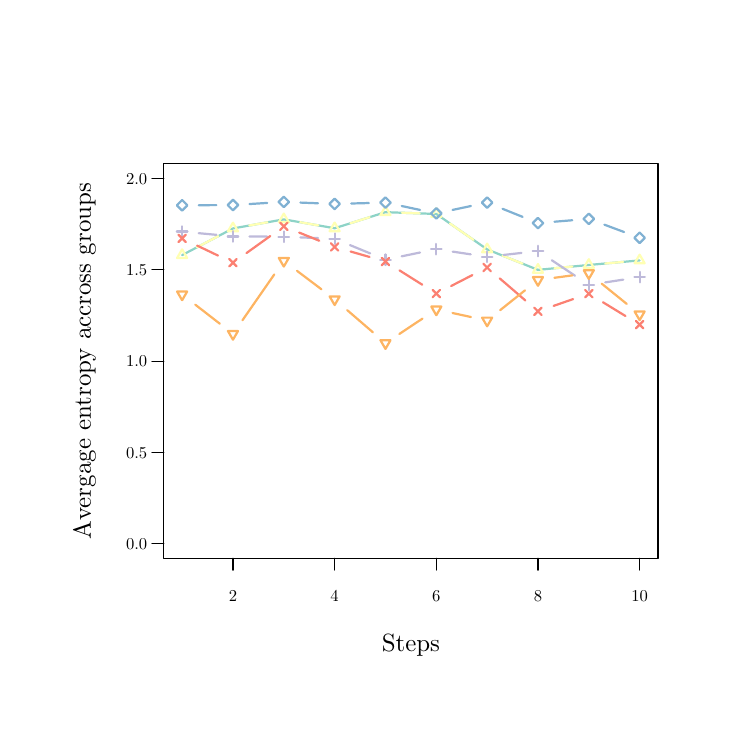
\begin{tikzpicture}[x=1pt,y=1pt]
\definecolor{fillColor}{RGB}{255,255,255}
\path[use as bounding box,fill=fillColor,fill opacity=0.00] (0,0) rectangle (252.94,252.94);
\begin{scope}
\path[clip] ( 49.20, 61.20) rectangle (227.75,203.75);
\definecolor{drawColor}{RGB}{141,211,199}

\path[draw=drawColor,line width= 0.8pt,line join=round,line cap=round] ( 55.81,170.76) --
	( 74.18,180.39) --
	( 92.55,183.67) --
	(110.92,180.46) --
	(129.29,186.27) --
	(147.66,185.62) --
	(166.03,172.82) --
	(184.39,165.42) --
	(202.76,167.19) --
	(221.13,168.84);
\end{scope}
\begin{scope}
\path[clip] (  0.00,  0.00) rectangle (252.94,252.94);
\definecolor{drawColor}{RGB}{0,0,0}

\path[draw=drawColor,line width= 0.4pt,line join=round,line cap=round] ( 74.18, 61.20) -- (221.13, 61.20);

\path[draw=drawColor,line width= 0.4pt,line join=round,line cap=round] ( 74.18, 61.20) -- ( 74.18, 56.92);

\path[draw=drawColor,line width= 0.4pt,line join=round,line cap=round] (110.92, 61.20) -- (110.92, 56.92);

\path[draw=drawColor,line width= 0.4pt,line join=round,line cap=round] (147.66, 61.20) -- (147.66, 56.92);

\path[draw=drawColor,line width= 0.4pt,line join=round,line cap=round] (184.39, 61.20) -- (184.39, 56.92);

\path[draw=drawColor,line width= 0.4pt,line join=round,line cap=round] (221.13, 61.20) -- (221.13, 56.92);

\node[text=drawColor,anchor=base,inner sep=0pt, outer sep=0pt, scale=  0.60] at ( 74.18, 45.60) {2};

\node[text=drawColor,anchor=base,inner sep=0pt, outer sep=0pt, scale=  0.60] at (110.92, 45.60) {4};

\node[text=drawColor,anchor=base,inner sep=0pt, outer sep=0pt, scale=  0.60] at (147.66, 45.60) {6};

\node[text=drawColor,anchor=base,inner sep=0pt, outer sep=0pt, scale=  0.60] at (184.39, 45.60) {8};

\node[text=drawColor,anchor=base,inner sep=0pt, outer sep=0pt, scale=  0.60] at (221.13, 45.60) {10};

\path[draw=drawColor,line width= 0.4pt,line join=round,line cap=round] ( 49.20, 66.48) -- ( 49.20,198.47);

\path[draw=drawColor,line width= 0.4pt,line join=round,line cap=round] ( 49.20, 66.48) -- ( 44.92, 66.48);

\path[draw=drawColor,line width= 0.4pt,line join=round,line cap=round] ( 49.20, 99.48) -- ( 44.92, 99.48);

\path[draw=drawColor,line width= 0.4pt,line join=round,line cap=round] ( 49.20,132.47) -- ( 44.92,132.47);

\path[draw=drawColor,line width= 0.4pt,line join=round,line cap=round] ( 49.20,165.47) -- ( 44.92,165.47);

\path[draw=drawColor,line width= 0.4pt,line join=round,line cap=round] ( 49.20,198.47) -- ( 44.92,198.47);

\node[text=drawColor,anchor=base east,inner sep=0pt, outer sep=0pt, scale=  0.60] at ( 43.20, 64.41) {0.0};

\node[text=drawColor,anchor=base east,inner sep=0pt, outer sep=0pt, scale=  0.60] at ( 43.20, 97.41) {0.5};

\node[text=drawColor,anchor=base east,inner sep=0pt, outer sep=0pt, scale=  0.60] at ( 43.20,130.41) {1.0};

\node[text=drawColor,anchor=base east,inner sep=0pt, outer sep=0pt, scale=  0.60] at ( 43.20,163.40) {1.5};

\node[text=drawColor,anchor=base east,inner sep=0pt, outer sep=0pt, scale=  0.60] at ( 43.20,196.40) {2.0};

\path[draw=drawColor,line width= 0.4pt,line join=round,line cap=round] ( 49.20, 61.20) --
	(227.75, 61.20) --
	(227.75,203.75) --
	( 49.20,203.75) --
	( 49.20, 61.20);
\end{scope}
\begin{scope}
\path[clip] (  0.00,  0.00) rectangle (252.94,252.94);
\definecolor{drawColor}{RGB}{0,0,0}

\node[text=drawColor,anchor=base,inner sep=0pt, outer sep=0pt, scale=  0.90] at (138.47, 27.60) {Steps};

\node[text=drawColor,rotate= 90.00,anchor=base,inner sep=0pt, outer sep=0pt, scale=  0.90] at ( 22.80,132.47) {Avergage entropy accross groups};
\end{scope}
\begin{scope}
\path[clip] ( 49.20, 61.20) rectangle (227.75,203.75);
\definecolor{drawColor}{RGB}{255,255,179}

\path[draw=drawColor,line width= 0.8pt,line join=round,line cap=round] ( 61.13,173.55) -- ( 68.87,177.61);

\path[draw=drawColor,line width= 0.8pt,line join=round,line cap=round] ( 80.09,181.45) -- ( 86.64,182.62);

\path[draw=drawColor,line width= 0.8pt,line join=round,line cap=round] ( 98.46,182.64) -- (105.01,181.49);

\path[draw=drawColor,line width= 0.8pt,line join=round,line cap=round] (116.64,182.27) -- (123.57,184.46);

\path[draw=drawColor,line width= 0.8pt,line join=round,line cap=round] (135.28,186.06) -- (141.66,185.83);

\path[draw=drawColor,line width= 0.8pt,line join=round,line cap=round] (152.58,182.19) -- (161.10,176.25);

\path[draw=drawColor,line width= 0.8pt,line join=round,line cap=round] (171.59,170.58) -- (178.83,167.66);

\path[draw=drawColor,line width= 0.8pt,line join=round,line cap=round] (190.37,166.00) -- (196.79,166.62);

\path[draw=drawColor,line width= 0.8pt,line join=round,line cap=round] (208.74,167.73) -- (215.16,168.30);

\path[draw=drawColor,line width= 0.8pt,line join=round,line cap=round] ( 55.81,172.86) --
	( 57.63,169.71) --
	( 53.99,169.71) --
	( 55.81,172.86);

\path[draw=drawColor,line width= 0.8pt,line join=round,line cap=round] ( 74.18,182.49) --
	( 76.00,179.34) --
	( 72.36,179.34) --
	( 74.18,182.49);

\path[draw=drawColor,line width= 0.8pt,line join=round,line cap=round] ( 92.55,185.77) --
	( 94.37,182.62) --
	( 90.73,182.62) --
	( 92.55,185.77);

\path[draw=drawColor,line width= 0.8pt,line join=round,line cap=round] (110.92,182.55) --
	(112.74,179.41) --
	(109.10,179.41) --
	(110.92,182.55);

\path[draw=drawColor,line width= 0.8pt,line join=round,line cap=round] (129.29,188.37) --
	(131.11,185.22) --
	(127.47,185.22) --
	(129.29,188.37);

\path[draw=drawColor,line width= 0.8pt,line join=round,line cap=round] (147.66,187.72) --
	(149.48,184.57) --
	(145.84,184.57) --
	(147.66,187.72);

\path[draw=drawColor,line width= 0.8pt,line join=round,line cap=round] (166.03,174.92) --
	(167.84,171.77) --
	(164.21,171.77) --
	(166.03,174.92);

\path[draw=drawColor,line width= 0.8pt,line join=round,line cap=round] (184.39,167.52) --
	(186.21,164.37) --
	(182.58,164.37) --
	(184.39,167.52);

\path[draw=drawColor,line width= 0.8pt,line join=round,line cap=round] (202.76,169.29) --
	(204.58,166.14) --
	(200.95,166.14) --
	(202.76,169.29);

\path[draw=drawColor,line width= 0.8pt,line join=round,line cap=round] (221.13,170.94) --
	(222.95,167.79) --
	(219.31,167.79) --
	(221.13,170.94);
\definecolor{drawColor}{RGB}{190,186,218}

\path[draw=drawColor,line width= 0.8pt,line join=round,line cap=round] ( 61.79,178.68) -- ( 68.21,178.08);

\path[draw=drawColor,line width= 0.8pt,line join=round,line cap=round] ( 80.18,177.48) -- ( 86.55,177.44);

\path[draw=drawColor,line width= 0.8pt,line join=round,line cap=round] ( 98.55,177.16) -- (104.92,176.90);

\path[draw=drawColor,line width= 0.8pt,line join=round,line cap=round] (116.47,174.37) -- (123.74,171.38);

\path[draw=drawColor,line width= 0.8pt,line join=round,line cap=round] (135.16,170.32) -- (141.78,171.69);

\path[draw=drawColor,line width= 0.8pt,line join=round,line cap=round] (153.59,172.01) -- (160.09,171.03);

\path[draw=drawColor,line width= 0.8pt,line join=round,line cap=round] (171.99,170.81) -- (178.43,171.54);

\path[draw=drawColor,line width= 0.8pt,line join=round,line cap=round] (189.39,168.89) -- (197.77,163.31);

\path[draw=drawColor,line width= 0.8pt,line join=round,line cap=round] (208.69,160.89) -- (215.20,161.89);

\path[draw=drawColor,line width= 0.8pt,line join=round,line cap=round] ( 53.90,179.25) -- ( 57.72,179.25);

\path[draw=drawColor,line width= 0.8pt,line join=round,line cap=round] ( 55.81,177.34) -- ( 55.81,181.16);

\path[draw=drawColor,line width= 0.8pt,line join=round,line cap=round] ( 72.27,177.51) -- ( 76.09,177.51);

\path[draw=drawColor,line width= 0.8pt,line join=round,line cap=round] ( 74.18,175.60) -- ( 74.18,179.42);

\path[draw=drawColor,line width= 0.8pt,line join=round,line cap=round] ( 90.64,177.40) -- ( 94.46,177.40);

\path[draw=drawColor,line width= 0.8pt,line join=round,line cap=round] ( 92.55,175.49) -- ( 92.55,179.31);

\path[draw=drawColor,line width= 0.8pt,line join=round,line cap=round] (109.01,176.65) -- (112.83,176.65);

\path[draw=drawColor,line width= 0.8pt,line join=round,line cap=round] (110.92,174.74) -- (110.92,178.56);

\path[draw=drawColor,line width= 0.8pt,line join=round,line cap=round] (127.38,169.10) -- (131.20,169.10);

\path[draw=drawColor,line width= 0.8pt,line join=round,line cap=round] (129.29,167.19) -- (129.29,171.01);

\path[draw=drawColor,line width= 0.8pt,line join=round,line cap=round] (145.75,172.91) -- (149.57,172.91);

\path[draw=drawColor,line width= 0.8pt,line join=round,line cap=round] (147.66,171.00) -- (147.66,174.82);

\path[draw=drawColor,line width= 0.8pt,line join=round,line cap=round] (164.12,170.13) -- (167.93,170.13);

\path[draw=drawColor,line width= 0.8pt,line join=round,line cap=round] (166.03,168.22) -- (166.03,172.04);

\path[draw=drawColor,line width= 0.8pt,line join=round,line cap=round] (182.49,172.22) -- (186.30,172.22);

\path[draw=drawColor,line width= 0.8pt,line join=round,line cap=round] (184.39,170.31) -- (184.39,174.12);

\path[draw=drawColor,line width= 0.8pt,line join=round,line cap=round] (200.85,159.98) -- (204.67,159.98);

\path[draw=drawColor,line width= 0.8pt,line join=round,line cap=round] (202.76,158.07) -- (202.76,161.89);

\path[draw=drawColor,line width= 0.8pt,line join=round,line cap=round] (219.22,162.80) -- (223.04,162.80);

\path[draw=drawColor,line width= 0.8pt,line join=round,line cap=round] (221.13,160.89) -- (221.13,164.71);
\definecolor{drawColor}{RGB}{251,128,114}

\path[draw=drawColor,line width= 0.8pt,line join=round,line cap=round] ( 61.23,174.20) -- ( 68.77,170.59);

\path[draw=drawColor,line width= 0.8pt,line join=round,line cap=round] ( 79.06,171.49) -- ( 87.67,177.65);

\path[draw=drawColor,line width= 0.8pt,line join=round,line cap=round] ( 98.11,178.89) -- (105.36,175.95);

\path[draw=drawColor,line width= 0.8pt,line join=round,line cap=round] (116.69,172.05) -- (123.52,170.09);

\path[draw=drawColor,line width= 0.8pt,line join=round,line cap=round] (134.36,165.23) -- (142.58,160.06);

\path[draw=drawColor,line width= 0.8pt,line join=round,line cap=round] (153.00,159.59) -- (160.69,163.53);

\path[draw=drawColor,line width= 0.8pt,line join=round,line cap=round] (170.57,162.35) -- (179.85,154.36);

\path[draw=drawColor,line width= 0.8pt,line join=round,line cap=round] (190.06,152.41) -- (197.10,154.86);

\path[draw=drawColor,line width= 0.8pt,line join=round,line cap=round] (207.89,153.71) -- (216.01,148.75);

\path[draw=drawColor,line width= 0.8pt,line join=round,line cap=round] ( 54.46,175.43) -- ( 57.16,178.13);

\path[draw=drawColor,line width= 0.8pt,line join=round,line cap=round] ( 54.46,178.13) -- ( 57.16,175.43);

\path[draw=drawColor,line width= 0.8pt,line join=round,line cap=round] ( 72.83,166.65) -- ( 75.53,169.35);

\path[draw=drawColor,line width= 0.8pt,line join=round,line cap=round] ( 72.83,169.35) -- ( 75.53,166.65);

\path[draw=drawColor,line width= 0.8pt,line join=round,line cap=round] ( 91.20,179.79) -- ( 93.90,182.49);

\path[draw=drawColor,line width= 0.8pt,line join=round,line cap=round] ( 91.20,182.49) -- ( 93.90,179.79);

\path[draw=drawColor,line width= 0.8pt,line join=round,line cap=round] (109.57,172.35) -- (112.27,175.05);

\path[draw=drawColor,line width= 0.8pt,line join=round,line cap=round] (109.57,175.05) -- (112.27,172.35);

\path[draw=drawColor,line width= 0.8pt,line join=round,line cap=round] (127.94,167.08) -- (130.64,169.78);

\path[draw=drawColor,line width= 0.8pt,line join=round,line cap=round] (127.94,169.78) -- (130.64,167.08);

\path[draw=drawColor,line width= 0.8pt,line join=round,line cap=round] (146.31,155.51) -- (149.01,158.21);

\path[draw=drawColor,line width= 0.8pt,line join=round,line cap=round] (146.31,158.21) -- (149.01,155.51);

\path[draw=drawColor,line width= 0.8pt,line join=round,line cap=round] (164.68,164.92) -- (167.38,167.62);

\path[draw=drawColor,line width= 0.8pt,line join=round,line cap=round] (164.68,167.62) -- (167.38,164.92);

\path[draw=drawColor,line width= 0.8pt,line join=round,line cap=round] (183.04,149.09) -- (185.74,151.79);

\path[draw=drawColor,line width= 0.8pt,line join=round,line cap=round] (183.04,151.79) -- (185.74,149.09);

\path[draw=drawColor,line width= 0.8pt,line join=round,line cap=round] (201.41,155.48) -- (204.11,158.18);

\path[draw=drawColor,line width= 0.8pt,line join=round,line cap=round] (201.41,158.18) -- (204.11,155.48);

\path[draw=drawColor,line width= 0.8pt,line join=round,line cap=round] (219.78,144.28) -- (222.48,146.98);

\path[draw=drawColor,line width= 0.8pt,line join=round,line cap=round] (219.78,146.98) -- (222.48,144.28);
\definecolor{drawColor}{RGB}{128,177,211}

\path[draw=drawColor,line width= 0.8pt,line join=round,line cap=round] ( 61.81,188.79) -- ( 68.18,188.82);

\path[draw=drawColor,line width= 0.8pt,line join=round,line cap=round] ( 80.17,189.21) -- ( 86.56,189.61);

\path[draw=drawColor,line width= 0.8pt,line join=round,line cap=round] ( 98.55,189.73) -- (104.92,189.48);

\path[draw=drawColor,line width= 0.8pt,line join=round,line cap=round] (116.92,189.40) -- (123.29,189.57);

\path[draw=drawColor,line width= 0.8pt,line join=round,line cap=round] (135.16,188.49) -- (141.79,187.08);

\path[draw=drawColor,line width= 0.8pt,line join=round,line cap=round] (153.53,187.08) -- (160.16,188.49);

\path[draw=drawColor,line width= 0.8pt,line join=round,line cap=round] (171.59,187.49) -- (178.83,184.57);

\path[draw=drawColor,line width= 0.8pt,line join=round,line cap=round] (190.37,182.82) -- (196.78,183.35);

\path[draw=drawColor,line width= 0.8pt,line join=round,line cap=round] (208.39,181.75) -- (215.51,179.10);

\path[draw=drawColor,line width= 0.8pt,line join=round,line cap=round] ( 53.90,188.76) --
	( 55.81,190.66) --
	( 57.72,188.76) --
	( 55.81,186.85) --
	( 53.90,188.76);

\path[draw=drawColor,line width= 0.8pt,line join=round,line cap=round] ( 72.27,188.85) --
	( 74.18,190.76) --
	( 76.09,188.85) --
	( 74.18,186.94) --
	( 72.27,188.85);

\path[draw=drawColor,line width= 0.8pt,line join=round,line cap=round] ( 90.64,189.97) --
	( 92.55,191.88) --
	( 94.46,189.97) --
	( 92.55,188.07) --
	( 90.64,189.97);

\path[draw=drawColor,line width= 0.8pt,line join=round,line cap=round] (109.01,189.24) --
	(110.92,191.15) --
	(112.83,189.24) --
	(110.92,187.33) --
	(109.01,189.24);

\path[draw=drawColor,line width= 0.8pt,line join=round,line cap=round] (127.38,189.73) --
	(129.29,191.64) --
	(131.20,189.73) --
	(129.29,187.83) --
	(127.38,189.73);

\path[draw=drawColor,line width= 0.8pt,line join=round,line cap=round] (145.75,185.83) --
	(147.66,187.74) --
	(149.57,185.83) --
	(147.66,183.92) --
	(145.75,185.83);

\path[draw=drawColor,line width= 0.8pt,line join=round,line cap=round] (164.12,189.73) --
	(166.03,191.64) --
	(167.93,189.73) --
	(166.03,187.83) --
	(164.12,189.73);

\path[draw=drawColor,line width= 0.8pt,line join=round,line cap=round] (182.49,182.33) --
	(184.39,184.24) --
	(186.30,182.33) --
	(184.39,180.42) --
	(182.49,182.33);

\path[draw=drawColor,line width= 0.8pt,line join=round,line cap=round] (200.85,183.85) --
	(202.76,185.76) --
	(204.67,183.85) --
	(202.76,181.94) --
	(200.85,183.85);

\path[draw=drawColor,line width= 0.8pt,line join=round,line cap=round] (219.22,177.01) --
	(221.13,178.92) --
	(223.04,177.01) --
	(221.13,175.10) --
	(219.22,177.01);
\definecolor{drawColor}{RGB}{253,180,98}

\path[draw=drawColor,line width= 0.8pt,line join=round,line cap=round] ( 60.55,152.86) -- ( 69.44,145.96);

\path[draw=drawColor,line width= 0.8pt,line join=round,line cap=round] ( 77.61,147.21) -- ( 89.12,163.77);

\path[draw=drawColor,line width= 0.8pt,line join=round,line cap=round] ( 97.33,165.07) -- (106.14,158.41);

\path[draw=drawColor,line width= 0.8pt,line join=round,line cap=round] (115.46,150.87) -- (124.74,142.87);

\path[draw=drawColor,line width= 0.8pt,line join=round,line cap=round] (134.29,142.26) -- (142.65,147.80);

\path[draw=drawColor,line width= 0.8pt,line join=round,line cap=round] (153.52,149.83) -- (160.16,148.39);

\path[draw=drawColor,line width= 0.8pt,line join=round,line cap=round] (170.72,150.85) -- (179.70,158.02);

\path[draw=drawColor,line width= 0.8pt,line join=round,line cap=round] (190.34,162.56) -- (196.82,163.43);

\path[draw=drawColor,line width= 0.8pt,line join=round,line cap=round] (207.42,160.45) -- (216.47,153.12);

\path[draw=drawColor,line width= 0.8pt,line join=round,line cap=round] ( 55.81,154.44) --
	( 57.63,157.59) --
	( 53.99,157.59) --
	( 55.81,154.44);

\path[draw=drawColor,line width= 0.8pt,line join=round,line cap=round] ( 74.18,140.18) --
	( 76.00,143.33) --
	( 72.36,143.33) --
	( 74.18,140.18);

\path[draw=drawColor,line width= 0.8pt,line join=round,line cap=round] ( 92.55,166.60) --
	( 94.37,169.74) --
	( 90.73,169.74) --
	( 92.55,166.60);

\path[draw=drawColor,line width= 0.8pt,line join=round,line cap=round] (110.92,152.69) --
	(112.74,155.83) --
	(109.10,155.83) --
	(110.92,152.69);

\path[draw=drawColor,line width= 0.8pt,line join=round,line cap=round] (129.29,136.85) --
	(131.11,140.00) --
	(127.47,140.00) --
	(129.29,136.85);

\path[draw=drawColor,line width= 0.8pt,line join=round,line cap=round] (147.66,149.01) --
	(149.48,152.16) --
	(145.84,152.16) --
	(147.66,149.01);

\path[draw=drawColor,line width= 0.8pt,line join=round,line cap=round] (166.03,145.01) --
	(167.84,148.16) --
	(164.21,148.16) --
	(166.03,145.01);

\path[draw=drawColor,line width= 0.8pt,line join=round,line cap=round] (184.39,159.66) --
	(186.21,162.81) --
	(182.58,162.81) --
	(184.39,159.66);

\path[draw=drawColor,line width= 0.8pt,line join=round,line cap=round] (202.76,162.13) --
	(204.58,165.28) --
	(200.95,165.28) --
	(202.76,162.13);

\path[draw=drawColor,line width= 0.8pt,line join=round,line cap=round] (221.13,147.24) --
	(222.95,150.39) --
	(219.31,150.39) --
	(221.13,147.24);
\end{scope}
\end{tikzpicture}
 & % Created by tikzDevice version 0.10.1 on 2016-06-29 16:09:48
% !TEX encoding = UTF-8 Unicode
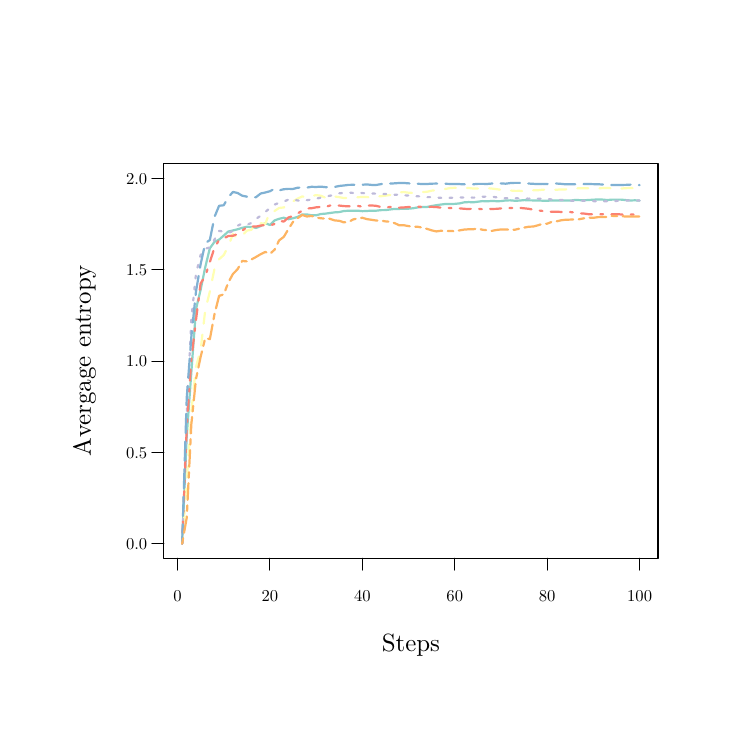
\begin{tikzpicture}[x=1pt,y=1pt]
\definecolor{fillColor}{RGB}{255,255,255}
\path[use as bounding box,fill=fillColor,fill opacity=0.00] (0,0) rectangle (252.94,252.94);
\begin{scope}
\path[clip] ( 49.20, 61.20) rectangle (227.75,203.75);
\definecolor{drawColor}{RGB}{141,211,199}

\path[draw=drawColor,line width= 0.8pt,line join=round,line cap=round] ( 55.81, 66.48) --
	( 57.48,105.48) --
	( 59.15,128.55) --
	( 60.82,151.21) --
	( 62.49,158.21) --
	( 64.16,166.36) --
	( 65.83,173.24) --
	( 67.50,175.53) --
	( 69.17,176.36) --
	( 70.84,177.80) --
	( 72.51,179.29) --
	( 74.18,179.66) --
	( 75.85,180.08) --
	( 77.52,180.61) --
	( 79.19,180.97) --
	( 80.86,180.93) --
	( 82.53,180.57) --
	( 84.20,181.25) --
	( 85.87,182.30) --
	( 87.54,181.63) --
	( 89.21,183.28) --
	( 90.88,183.88) --
	( 92.55,184.25) --
	( 94.22,183.73) --
	( 95.89,184.07) --
	( 97.56,184.57) --
	( 99.23,185.45) --
	(100.90,185.44) --
	(102.57,185.15) --
	(104.24,185.14) --
	(105.91,185.60) --
	(107.58,185.74) --
	(109.25,185.97) --
	(110.92,186.20) --
	(112.59,186.30) --
	(114.26,186.69) --
	(115.93,186.78) --
	(117.60,186.80) --
	(119.27,186.81) --
	(120.94,186.63) --
	(122.61,186.71) --
	(124.28,186.81) --
	(125.95,186.81) --
	(127.62,187.00) --
	(129.29,187.02) --
	(130.96,187.24) --
	(132.63,187.45) --
	(134.30,187.45) --
	(135.97,187.49) --
	(137.64,187.54) --
	(139.31,187.69) --
	(140.98,187.99) --
	(142.65,188.12) --
	(144.32,188.15) --
	(145.99,188.49) --
	(147.66,188.79) --
	(149.33,189.03) --
	(151.00,189.23) --
	(152.67,189.20) --
	(154.34,189.27) --
	(156.01,189.43) --
	(157.68,189.81) --
	(159.35,189.92) --
	(161.02,189.83) --
	(162.69,190.05) --
	(164.36,190.27) --
	(166.03,190.19) --
	(167.70,190.32) --
	(169.37,190.24) --
	(171.04,190.26) --
	(172.71,190.50) --
	(174.38,190.54) --
	(176.05,190.40) --
	(177.71,190.45) --
	(179.38,190.63) --
	(181.05,190.54) --
	(182.72,190.52) --
	(184.39,190.45) --
	(186.06,190.43) --
	(187.73,190.40) --
	(189.40,190.48) --
	(191.07,190.48) --
	(192.74,190.50) --
	(194.41,190.52) --
	(196.08,190.45) --
	(197.75,190.68) --
	(199.42,190.62) --
	(201.09,190.57) --
	(202.76,190.68) --
	(204.43,190.77) --
	(206.10,190.89) --
	(207.77,190.81) --
	(209.44,190.65) --
	(211.11,190.80) --
	(212.78,190.80) --
	(214.45,190.80) --
	(216.12,190.63) --
	(217.79,190.50) --
	(219.46,190.55) --
	(221.13,190.44);
\end{scope}
\begin{scope}
\path[clip] (  0.00,  0.00) rectangle (252.94,252.94);
\definecolor{drawColor}{RGB}{0,0,0}

\path[draw=drawColor,line width= 0.4pt,line join=round,line cap=round] ( 54.14, 61.20) -- (221.13, 61.20);

\path[draw=drawColor,line width= 0.4pt,line join=round,line cap=round] ( 54.14, 61.20) -- ( 54.14, 56.92);

\path[draw=drawColor,line width= 0.4pt,line join=round,line cap=round] ( 87.54, 61.20) -- ( 87.54, 56.92);

\path[draw=drawColor,line width= 0.4pt,line join=round,line cap=round] (120.94, 61.20) -- (120.94, 56.92);

\path[draw=drawColor,line width= 0.4pt,line join=round,line cap=round] (154.34, 61.20) -- (154.34, 56.92);

\path[draw=drawColor,line width= 0.4pt,line join=round,line cap=round] (187.73, 61.20) -- (187.73, 56.92);

\path[draw=drawColor,line width= 0.4pt,line join=round,line cap=round] (221.13, 61.20) -- (221.13, 56.92);

\node[text=drawColor,anchor=base,inner sep=0pt, outer sep=0pt, scale=  0.60] at ( 54.14, 45.60) {0};

\node[text=drawColor,anchor=base,inner sep=0pt, outer sep=0pt, scale=  0.60] at ( 87.54, 45.60) {20};

\node[text=drawColor,anchor=base,inner sep=0pt, outer sep=0pt, scale=  0.60] at (120.94, 45.60) {40};

\node[text=drawColor,anchor=base,inner sep=0pt, outer sep=0pt, scale=  0.60] at (154.34, 45.60) {60};

\node[text=drawColor,anchor=base,inner sep=0pt, outer sep=0pt, scale=  0.60] at (187.73, 45.60) {80};

\node[text=drawColor,anchor=base,inner sep=0pt, outer sep=0pt, scale=  0.60] at (221.13, 45.60) {100};

\path[draw=drawColor,line width= 0.4pt,line join=round,line cap=round] ( 49.20, 66.48) -- ( 49.20,198.47);

\path[draw=drawColor,line width= 0.4pt,line join=round,line cap=round] ( 49.20, 66.48) -- ( 44.92, 66.48);

\path[draw=drawColor,line width= 0.4pt,line join=round,line cap=round] ( 49.20, 99.48) -- ( 44.92, 99.48);

\path[draw=drawColor,line width= 0.4pt,line join=round,line cap=round] ( 49.20,132.47) -- ( 44.92,132.47);

\path[draw=drawColor,line width= 0.4pt,line join=round,line cap=round] ( 49.20,165.47) -- ( 44.92,165.47);

\path[draw=drawColor,line width= 0.4pt,line join=round,line cap=round] ( 49.20,198.47) -- ( 44.92,198.47);

\node[text=drawColor,anchor=base east,inner sep=0pt, outer sep=0pt, scale=  0.60] at ( 43.20, 64.41) {0.0};

\node[text=drawColor,anchor=base east,inner sep=0pt, outer sep=0pt, scale=  0.60] at ( 43.20, 97.41) {0.5};

\node[text=drawColor,anchor=base east,inner sep=0pt, outer sep=0pt, scale=  0.60] at ( 43.20,130.41) {1.0};

\node[text=drawColor,anchor=base east,inner sep=0pt, outer sep=0pt, scale=  0.60] at ( 43.20,163.40) {1.5};

\node[text=drawColor,anchor=base east,inner sep=0pt, outer sep=0pt, scale=  0.60] at ( 43.20,196.40) {2.0};

\path[draw=drawColor,line width= 0.4pt,line join=round,line cap=round] ( 49.20, 61.20) --
	(227.75, 61.20) --
	(227.75,203.75) --
	( 49.20,203.75) --
	( 49.20, 61.20);
\end{scope}
\begin{scope}
\path[clip] (  0.00,  0.00) rectangle (252.94,252.94);
\definecolor{drawColor}{RGB}{0,0,0}

\node[text=drawColor,anchor=base,inner sep=0pt, outer sep=0pt, scale=  0.90] at (138.47, 27.60) {Steps};

\node[text=drawColor,rotate= 90.00,anchor=base,inner sep=0pt, outer sep=0pt, scale=  0.90] at ( 22.80,132.47) {Avergage entropy};
\end{scope}
\begin{scope}
\path[clip] ( 49.20, 61.20) rectangle (227.75,203.75);
\definecolor{drawColor}{RGB}{255,255,179}

\path[draw=drawColor,line width= 0.8pt,dash pattern=on 4pt off 4pt ,line join=round,line cap=round] ( 55.81, 66.48) --
	( 57.48, 88.48) --
	( 59.15,114.21) --
	( 60.82,130.40) --
	( 62.49,136.40) --
	( 64.16,150.88) --
	( 65.83,157.60) --
	( 67.50,165.78) --
	( 69.17,169.28) --
	( 70.84,170.76) --
	( 72.51,173.95) --
	( 74.18,178.42) --
	( 75.85,176.74) --
	( 77.52,177.76) --
	( 79.19,179.60) --
	( 80.86,179.90) --
	( 82.53,182.58) --
	( 84.20,182.27) --
	( 85.87,182.08) --
	( 87.54,186.41) --
	( 89.21,186.68) --
	( 90.88,187.80) --
	( 92.55,187.97) --
	( 94.22,189.39) --
	( 95.89,190.17) --
	( 97.56,191.18) --
	( 99.23,191.95) --
	(100.90,191.57) --
	(102.57,192.08) --
	(104.24,192.43) --
	(105.91,192.22) --
	(107.58,191.49) --
	(109.25,192.16) --
	(110.92,191.93) --
	(112.59,191.69) --
	(114.26,191.36) --
	(115.93,191.42) --
	(117.60,191.47) --
	(119.27,191.66) --
	(120.94,191.77) --
	(122.61,191.72) --
	(124.28,191.60) --
	(125.95,191.98) --
	(127.62,192.03) --
	(129.29,192.24) --
	(130.96,192.46) --
	(132.63,192.98) --
	(134.30,193.45) --
	(135.97,193.53) --
	(137.64,193.30) --
	(139.31,193.22) --
	(140.98,193.25) --
	(142.65,193.53) --
	(144.32,193.64) --
	(145.99,194.04) --
	(147.66,194.22) --
	(149.33,194.47) --
	(151.00,194.68) --
	(152.67,194.98) --
	(154.34,195.08) --
	(156.01,195.04) --
	(157.68,195.02) --
	(159.35,195.01) --
	(161.02,194.80) --
	(162.69,194.79) --
	(164.36,194.89) --
	(166.03,194.95) --
	(167.70,194.80) --
	(169.37,194.60) --
	(171.04,194.35) --
	(172.71,194.20) --
	(174.38,194.10) --
	(176.05,193.96) --
	(177.71,193.98) --
	(179.38,193.84) --
	(181.05,193.95) --
	(182.72,194.17) --
	(184.39,194.19) --
	(186.06,194.40) --
	(187.73,194.37) --
	(189.40,194.36) --
	(191.07,194.37) --
	(192.74,194.49) --
	(194.41,194.50) --
	(196.08,194.65) --
	(197.75,194.89) --
	(199.42,194.88) --
	(201.09,194.92) --
	(202.76,194.92) --
	(204.43,194.82) --
	(206.10,194.90) --
	(207.77,194.97) --
	(209.44,195.05) --
	(211.11,194.89) --
	(212.78,194.83) --
	(214.45,194.81) --
	(216.12,194.94) --
	(217.79,195.00) --
	(219.46,194.93) --
	(221.13,194.78);
\definecolor{drawColor}{RGB}{190,186,218}

\path[draw=drawColor,line width= 0.8pt,dash pattern=on 1pt off 3pt ,line join=round,line cap=round] ( 55.81, 66.48) --
	( 57.48,113.06) --
	( 59.15,147.78) --
	( 60.82,164.00) --
	( 62.49,170.78) --
	( 64.16,173.09) --
	( 65.83,173.52) --
	( 67.50,176.37) --
	( 69.17,179.51) --
	( 70.84,179.25) --
	( 72.51,178.77) --
	( 74.18,179.49) --
	( 75.85,181.38) --
	( 77.52,182.16) --
	( 79.19,181.72) --
	( 80.86,182.36) --
	( 82.53,183.89) --
	( 84.20,184.96) --
	( 85.87,186.39) --
	( 87.54,187.71) --
	( 89.21,189.00) --
	( 90.88,189.68) --
	( 92.55,190.11) --
	( 94.22,190.81) --
	( 95.89,190.76) --
	( 97.56,190.51) --
	( 99.23,190.15) --
	(100.90,190.60) --
	(102.57,190.82) --
	(104.24,191.15) --
	(105.91,191.51) --
	(107.58,191.94) --
	(109.25,192.21) --
	(110.92,192.60) --
	(112.59,193.07) --
	(114.26,193.23) --
	(115.93,193.35) --
	(117.60,193.22) --
	(119.27,193.35) --
	(120.94,193.16) --
	(122.61,193.11) --
	(124.28,193.03) --
	(125.95,192.95) --
	(127.62,192.78) --
	(129.29,192.85) --
	(130.96,192.72) --
	(132.63,192.54) --
	(134.30,192.65) --
	(135.97,192.37) --
	(137.64,192.29) --
	(139.31,192.06) --
	(140.98,192.00) --
	(142.65,191.90) --
	(144.32,191.70) --
	(145.99,191.70) --
	(147.66,191.58) --
	(149.33,191.45) --
	(151.00,191.25) --
	(152.67,191.46) --
	(154.34,191.57) --
	(156.01,191.64) --
	(157.68,191.53) --
	(159.35,191.58) --
	(161.02,191.52) --
	(162.69,191.58) --
	(164.36,191.86) --
	(166.03,191.90) --
	(167.70,191.89) --
	(169.37,191.64) --
	(171.04,191.40) --
	(172.71,191.31) --
	(174.38,191.38) --
	(176.05,191.28) --
	(177.71,191.25) --
	(179.38,191.21) --
	(181.05,191.16) --
	(182.72,191.23) --
	(184.39,191.16) --
	(186.06,191.13) --
	(187.73,191.04) --
	(189.40,190.85) --
	(191.07,190.69) --
	(192.74,190.70) --
	(194.41,190.60) --
	(196.08,190.40) --
	(197.75,190.34) --
	(199.42,190.46) --
	(201.09,190.40) --
	(202.76,190.33) --
	(204.43,190.26) --
	(206.10,190.18) --
	(207.77,190.16) --
	(209.44,190.20) --
	(211.11,190.27) --
	(212.78,190.34) --
	(214.45,190.42) --
	(216.12,190.46) --
	(217.79,190.51) --
	(219.46,190.51) --
	(221.13,190.45);
\definecolor{drawColor}{RGB}{251,128,114}

\path[draw=drawColor,line width= 0.8pt,dash pattern=on 1pt off 3pt on 4pt off 3pt ,line join=round,line cap=round] ( 55.81, 66.48) --
	( 57.48,108.48) --
	( 59.15,133.31) --
	( 60.82,147.27) --
	( 62.49,160.54) --
	( 64.16,163.12) --
	( 65.83,168.26) --
	( 67.50,173.44) --
	( 69.17,176.21) --
	( 70.84,176.78) --
	( 72.51,177.68) --
	( 74.18,177.74) --
	( 75.85,178.36) --
	( 77.52,179.52) --
	( 79.19,180.95) --
	( 80.86,181.06) --
	( 82.53,181.06) --
	( 84.20,181.44) --
	( 85.87,181.61) --
	( 87.54,181.42) --
	( 89.21,182.03) --
	( 90.88,183.13) --
	( 92.55,182.88) --
	( 94.22,184.34) --
	( 95.89,184.93) --
	( 97.56,185.80) --
	( 99.23,186.84) --
	(100.90,187.60) --
	(102.57,187.69) --
	(104.24,188.02) --
	(105.91,188.16) --
	(107.58,188.17) --
	(109.25,188.66) --
	(110.92,188.48) --
	(112.59,188.65) --
	(114.26,188.47) --
	(115.93,188.38) --
	(117.60,188.54) --
	(119.27,188.52) --
	(120.94,188.27) --
	(122.61,188.64) --
	(124.28,188.70) --
	(125.95,188.55) --
	(127.62,188.14) --
	(129.29,188.01) --
	(130.96,188.14) --
	(132.63,188.25) --
	(134.30,187.90) --
	(135.97,187.98) --
	(137.64,188.14) --
	(139.31,188.16) --
	(140.98,188.26) --
	(142.65,188.18) --
	(144.32,188.14) --
	(145.99,188.20) --
	(147.66,188.12) --
	(149.33,187.88) --
	(151.00,187.84) --
	(152.67,187.79) --
	(154.34,187.67) --
	(156.01,187.66) --
	(157.68,187.50) --
	(159.35,187.39) --
	(161.02,187.56) --
	(162.69,187.49) --
	(164.36,187.34) --
	(166.03,187.43) --
	(167.70,187.43) --
	(169.37,187.47) --
	(171.04,187.63) --
	(172.71,187.71) --
	(174.38,187.75) --
	(176.05,187.80) --
	(177.71,187.82) --
	(179.38,187.67) --
	(181.05,187.48) --
	(182.72,187.19) --
	(184.39,186.92) --
	(186.06,186.71) --
	(187.73,186.51) --
	(189.40,186.40) --
	(191.07,186.45) --
	(192.74,186.34) --
	(194.41,186.40) --
	(196.08,186.31) --
	(197.75,186.16) --
	(199.42,185.87) --
	(201.09,185.76) --
	(202.76,185.53) --
	(204.43,185.49) --
	(206.10,185.54) --
	(207.77,185.55) --
	(209.44,185.42) --
	(211.11,185.50) --
	(212.78,185.55) --
	(214.45,185.45) --
	(216.12,185.39) --
	(217.79,185.39) --
	(219.46,185.50) --
	(221.13,185.49);
\definecolor{drawColor}{RGB}{128,177,211}

\path[draw=drawColor,line width= 0.8pt,dash pattern=on 7pt off 3pt ,line join=round,line cap=round] ( 55.81, 66.48) --
	( 57.48,119.27) --
	( 59.15,141.36) --
	( 60.82,157.62) --
	( 62.49,167.43) --
	( 64.16,175.07) --
	( 65.83,176.19) --
	( 67.50,184.53) --
	( 69.17,188.58) --
	( 70.84,188.76) --
	( 72.51,191.69) --
	( 74.18,193.58) --
	( 75.85,193.20) --
	( 77.52,192.22) --
	( 79.19,191.88) --
	( 80.86,191.35) --
	( 82.53,191.70) --
	( 84.20,193.02) --
	( 85.87,193.38) --
	( 87.54,193.84) --
	( 89.21,194.74) --
	( 90.88,194.15) --
	( 92.55,194.56) --
	( 94.22,194.69) --
	( 95.89,194.66) --
	( 97.56,195.11) --
	( 99.23,195.19) --
	(100.90,195.16) --
	(102.57,195.44) --
	(104.24,195.37) --
	(105.91,195.50) --
	(107.58,195.31) --
	(109.25,195.30) --
	(110.92,195.38) --
	(112.59,195.74) --
	(114.26,195.91) --
	(115.93,196.13) --
	(117.60,196.15) --
	(119.27,196.24) --
	(120.94,196.19) --
	(122.61,196.28) --
	(124.28,196.12) --
	(125.95,196.10) --
	(127.62,196.39) --
	(129.29,196.66) --
	(130.96,196.60) --
	(132.63,196.69) --
	(134.30,196.82) --
	(135.97,196.82) --
	(137.64,196.68) --
	(139.31,196.58) --
	(140.98,196.53) --
	(142.65,196.44) --
	(144.32,196.45) --
	(145.99,196.57) --
	(147.66,196.60) --
	(149.33,196.60) --
	(151.00,196.52) --
	(152.67,196.47) --
	(154.34,196.48) --
	(156.01,196.42) --
	(157.68,196.33) --
	(159.35,196.47) --
	(161.02,196.35) --
	(162.69,196.50) --
	(164.36,196.50) --
	(166.03,196.46) --
	(167.70,196.61) --
	(169.37,196.75) --
	(171.04,196.67) --
	(172.71,196.56) --
	(174.38,196.78) --
	(176.05,196.86) --
	(177.71,196.86) --
	(179.38,196.73) --
	(181.05,196.61) --
	(182.72,196.51) --
	(184.39,196.41) --
	(186.06,196.49) --
	(187.73,196.45) --
	(189.40,196.58) --
	(191.07,196.61) --
	(192.74,196.50) --
	(194.41,196.33) --
	(196.08,196.34) --
	(197.75,196.33) --
	(199.42,196.37) --
	(201.09,196.45) --
	(202.76,196.43) --
	(204.43,196.40) --
	(206.10,196.35) --
	(207.77,196.27) --
	(209.44,196.18) --
	(211.11,196.06) --
	(212.78,196.06) --
	(214.45,196.12) --
	(216.12,196.13) --
	(217.79,196.22) --
	(219.46,196.15) --
	(221.13,196.05);
\definecolor{drawColor}{RGB}{253,180,98}

\path[draw=drawColor,line width= 0.8pt,dash pattern=on 2pt off 2pt on 6pt off 2pt ,line join=round,line cap=round] ( 55.81, 66.48) --
	( 57.48, 75.91) --
	( 59.15,109.77) --
	( 60.82,125.98) --
	( 62.49,133.95) --
	( 64.16,140.78) --
	( 65.83,140.38) --
	( 67.50,149.34) --
	( 69.17,156.03) --
	( 70.84,156.54) --
	( 72.51,160.88) --
	( 74.18,163.96) --
	( 75.85,165.66) --
	( 77.52,168.64) --
	( 79.19,168.48) --
	( 80.86,169.18) --
	( 82.53,170.09) --
	( 84.20,171.09) --
	( 85.87,171.89) --
	( 87.54,171.19) --
	( 89.21,172.71) --
	( 90.88,176.09) --
	( 92.55,177.34) --
	( 94.22,180.16) --
	( 95.89,182.78) --
	( 97.56,184.12) --
	( 99.23,185.26) --
	(100.90,184.70) --
	(102.57,184.91) --
	(104.24,184.34) --
	(105.91,184.06) --
	(107.58,183.95) --
	(109.25,183.86) --
	(110.92,183.30) --
	(112.59,183.14) --
	(114.26,182.58) --
	(115.93,182.72) --
	(117.60,183.63) --
	(119.27,184.04) --
	(120.94,184.24) --
	(122.61,183.75) --
	(124.28,183.51) --
	(125.95,183.25) --
	(127.62,183.23) --
	(129.29,182.94) --
	(130.96,182.80) --
	(132.63,182.30) --
	(134.30,181.51) --
	(135.97,181.54) --
	(137.64,181.23) --
	(139.31,181.06) --
	(140.98,180.99) --
	(142.65,180.67) --
	(144.32,180.23) --
	(145.99,179.70) --
	(147.66,179.31) --
	(149.33,179.55) --
	(151.00,179.41) --
	(152.67,179.50) --
	(154.34,179.37) --
	(156.01,179.67) --
	(157.68,179.97) --
	(159.35,180.09) --
	(161.02,180.10) --
	(162.69,180.39) --
	(164.36,179.90) --
	(166.03,179.75) --
	(167.70,179.50) --
	(169.37,179.83) --
	(171.04,180.03) --
	(172.71,180.03) --
	(174.38,179.90) --
	(176.05,179.92) --
	(177.71,180.32) --
	(179.38,180.69) --
	(181.05,181.01) --
	(182.72,181.08) --
	(184.39,181.53) --
	(186.06,182.06) --
	(187.73,182.12) --
	(189.40,182.76) --
	(191.07,182.95) --
	(192.74,183.33) --
	(194.41,183.54) --
	(196.08,183.58) --
	(197.75,183.70) --
	(199.42,183.75) --
	(201.09,184.06) --
	(202.76,184.31) --
	(204.43,184.24) --
	(206.10,184.47) --
	(207.77,184.53) --
	(209.44,184.52) --
	(211.11,184.94) --
	(212.78,184.85) --
	(214.45,184.83) --
	(216.12,184.70) --
	(217.79,184.69) --
	(219.46,184.71) --
	(221.13,184.74);
\end{scope}
\end{tikzpicture}
 \\
	(\textbf{c}) Block wise entropy  & (\textbf{d}) Cumulative entropy 
	\end{tabular} \quad
	\caption{Disadvantageous behaviour and entropy averaged by criminal profile }
	\label{fig:ent}
\end{figure}

\cite{Yechiam2008} found three clusters by using the attention to recent outcomes(ARO) and attention to gains(AG) parameters from the Expectancy Valance model. The most distinct group were the Robbery convicts with the only negative attention to gains mean at -0.36 and the highest attention to recent outcomes mean 0.57. The second cluster is made of assault and murder convicts with ARO of 0.26 and AG of 0.1. The third cluster is formed of all the remaining prisoner groups with ARO means between 0 and -0.1 and AG between 0.1 and 0.2.\\
Based on those findings and what we observed in figure \ref{fig:ent} we decided to cluster convicted assault-murder and robbery individuals against the other criminal groups. The following table depicts selected resulting clustering performance.\footnote{The remaining results can be found in table  \ref{tab:prison1} and \ref{tab:prison2} in the appendix} We find the most accurate clustering among all between assault/murders and forgery, both on entropy and and cumulative bad choices, which is suggested by the descriptive findings from figure \ref{fig:ent}. The listed algorithms performed remarkably better than the average performance. Furthermore, we managed to find some weaker clustering results between robbery. In contrast to \cite{Yechiam2008} we manged to isolate rather assault/murder criminals from the rest than robbery.

\begin{table}[!htbp] \centering 
	\caption{} 
	\label{} 
	\footnotesize
	\resizebox{\textwidth}{!}{\begin{tabular}{@{\extracolsep{0pt}} lllccccccccc} 
\toprule 
		\textbf{Groups} & \textbf{Method} & \textbf{Similarity} & \textbf{C} & \textbf{CBC} & \textbf{BBC} &\textbf{ E }& \textbf{EB} & \textbf{CC} & \textbf{NMI} & \textbf{ARI} & \textbf{VM} \\ 
		\hline 
				2 vs. 9 & Spectral & EDR &  &  &  & x &  &  & 0.382 (0.000) & 0.235 (0.000) & 0.382 (0.000)\\ 
				& Spectral & EDR &  &  & x &  &  &  & 0.232 (0.000) & 0.226 (0.000) & 0.232 (0.000)\\ 
				& Spectral & Cosine &  &  &  &  & x &  & 0.197 (0.000) & 0.008 (0.000)& 0.191 (0.000)\\ 
				& Spectral & RBF &  & x &  &  &  &  & 0.134 (0.000)& 0.075 (0.000)& 0.134 (0.000) \\ 
				& K-Means & Euclidean &  &  &  &  &  & x & 0.116 (0.000) & - & 0.105 (0.000) \\ 
				& K-Means & Euclidean & x &  &  &  &  &  & 0.111 (0.022) & - & 0.100 (0.020) \\
						\hline
						\textbf{Average} &  &  &  &  &  &  &  &  & \textbf{0.096 (0.074)} & \textbf{-} & \textbf{0.093 (0.073)} \\ 
				\hline 
		6 vs. 9 & Ward  & Euclidean &  &  &  &  & x &  & 0.561 (0.000) & 0.560 (0,000) & 0.560 (0,000) \\ 
		& Spectral & DTW &  &  &  & x &  &  & 0.435 (0.000) & 0.387 (0.000) & 0.432 (0.000) \\ 
		& Spectral & DTW &  & x &  &  &  &  & 0.435 (0.000) & 0.387 (0.000) & 0.432 (0.000) \\ 
		& Spectral & EDR &  &  & x &  &  &  & 0.333 (0.000) & 0.381 (0.000) & 0.333 (0.000) \\ 
		& Spectral & Overlap & x &  &  &  &  &  & 0.111 (0.000) & 0.118 (0.000) & 0.111 (0.000) \\ 
		& K-Means & Euclidean &  &  &  &  &  & x & 0.106 (0.066) & 0.033 (0.054) & 0.094 (0.059) \\
		\hline
		 \textbf{Average}& &  &  &  &  &  &  &  & \textbf{0.249 (0.167)} & \textbf{0.202 (0.189)} & \textbf{0.244 (0.169)} \\ 
		\hline \\[-1.8ex] 
	\end{tabular} }
\end{table} 

\subsection{Cocaine Abusers data}

Finally we study data from several cocaine abusers. There are 12 individuals performing the IGT. The control group consist out of 14 participants. Candidates among the drug abusers were selected as active users with additional drug abusing past, but without any known additional mental illness \cite{Stout2004}. Table \ref{tab:cocs} gives a summary of demographic profile.

\setlength{\tabcolsep}{12pt}
\renewcommand{\arraystretch}{1}
\begin{table}[H]
	\centering 
		\caption{Demographic summary of cocaine abusers (means with standard deviations in parenthesis)}
	\begin{tabular}{lcc}
		\toprule
		\textbf{Demographic indicator} & \textbf{Drug abusers} & \textbf{Control Group} \\
		\hline
		Share of men &  79\% & 100\%\\
		Age & 36.90 (10.30) & 30.00 (6.10) \\
		Estimated IQ & 105.00 (7.62) & 93.70 (10.30) \\
		\bottomrule
	\end{tabular}
	\label{tab:cocs}
\end{table}




Within the gambling task they found that cocaine abusers choose persistently cards from disadvantageous decks. The effect is still present after controlling for the low IQ score.\\
We cluster cocaine abusers against the control group. The following table \ref{tab:cocainresults} depicts results of the clustering. Again we averaged over 20 simulations to report overall clustering performance. However as depicted the data set is friarly small and results are quite stable.\\
Again our best clustering is achieved using block wise entropy, besides the listed K-Means algorithm, spectral clustering based on both cosine similarity and with rbf kernel achieved the same results. However, the results for this data set are rather low and we could not find  good clustering between the control group and cocaine abusers. This also is indicated by the average over all applied methods. 

\begin{threeparttable}[H] 
	\centering
	\label{} 
	\scriptsize
		\resizebox{\textwidth}{!}{\begin{tabular}{ llccc cccccc} 
		\toprule
			\textbf{Method} & \textbf{Similarity} & \textbf{C}\tnote{0} & \textbf{CBC}\tnote{1} & \textbf{BBC}\tnote{2} & \textbf{E}\tnote{3} & \textbf{EB}\tnote{4} & \textbf{CC}\tnote{5} & \textbf{NMI}\tnote{6} & \textbf{AR}I\tnote{6} & \textbf{VM}\tnote{7} \\ 
		\hline 
		K-Means \tnote{*} & Euclidean &  &  &  &  & x &  & 0.270 (0.000) & 0.262 (0.000) & 0.270 (0.000) \\ 
		Ward & Euclidean &  & x &  &  &  &  & 0.270 (0.000) & 0.262 (0.000) & 0.270 (0.000) \\ 
		K-Means & Euclidean &  &  &  &  &  & x & 0.209 (0.030) & 0.171 (0.043) & 0.208 (0.030) \\ 
		Spectral & Levenstein & x &  &  &  &  &  & 0.178 (0.000) & 0.181 (0.000) & 0.178 (0.000) \\ 
		Spectral & Cosine &  &  & x &  &  &  & 0.171 (0.000) & 0.117 (0.000) & 0.171 (0.000) \\ 
		Spectral & DTW &  &  &  & x &  &  & 0.042 (0,000) & 0.014 (0.000) & 0.042 (0.000) \\ 
		\hline
		\textbf{Average}\tnote{$\dagger$}  &  &  &  &  &  &  & & \textbf{0.139 (0.002)} & \textbf{0.104 (0.003)} & \textbf{0.138 (0.002)} \\ 
		\hline 
	\end{tabular} }
	\begin{tcolorbox}[arc=0mm,title=Notes,boxrule=0.2mm,colbacktitle=white,coltitle=black,colback=white,top=0mm,bottom=0.1mm]
	\begin{tablenotes}
	       	\item[0] Clustering based on choices participant did 
	       	\item[1] Clustering based on cumulative disadvantageous choice of participants
	        \item[2] Clustering based on block wise disadvantageous choice. Block size = 10
	        \item[3] Clustering based on cumulative entropy
	        \item[4] Clustering based on block wise entropy. Block size = 10
	        \item[5] Clustering based on entropy and choices concatenated for each participant
	        \item[6] Normalised mutual infrormation score (description see appendix \ref{sec:ce})
	        \item[7] Adjusted rand index (description see appendix \ref{sec:ce})
	        \item[8] V-Measure (description see appendix \ref{sec:ce})
	        \item[*] Spectral Clustering on block wise entropy with RBF kernel and cosine similarity produced the same results
	        \item[$\dagger$] Average over all algorithms including the ones displayed in the table
	\end{tablenotes}
	\end{tcolorbox}
	\caption{Clustering results for cocaine abusers vs. control group} 
	\label{tab:cocainresults}
 \end{threeparttable} 

\section{Discussion of results and possible extensions }

Our analysis so far showed that people are not separate themselves. In general we assume that healthy participants and those with assumed decision making deficits show significantly different behaviour. However, we observe that their behaviour seems to be quite similar given our data and applied mappings. Furthermore , in most of the applied unsupervised techniques we as analysts have to to set the number of clusters we assume to be in the data (so in our case two for control group and patients with habits). We apply another algorithm called affinity propagation, which identifies the number of clusters itself (algorithm formulation see appendix). In general we find that the algorithm is assigning many more clusters to our data. This suggests that there may be more natural clusters in the data instead of simply splitting by healthy and ill labels. This can be addressed by Bayesian nonparametric models. \cite{Gershman2012}

%---------------------------------------------------------------------------------------------------------
% 5. Data
%---------------------------------------------------------------------------------------------------------

\section{Conclusion}

Maybe process also reward data.

Our simulations show the RL parameter difference thresholds required for successful clustering given multi-armed bandit reward distribution. We also notice that $\tau$ has relatively much greater effect on individual's behaviour than the learning rate $\alpha$. Fitting unsupervised learning models on real experiment data reveals that they seldom discover the clusters in the parameter space of reinforcement learning models. 




\section{Acknowledgements}




\pagebreak
% ----------------------------------------------------------------------------------------------------------
% Literature
% ----------------------------------------------------------------------------------------------------------

\renewcommand\refname{List of Literature}

\bibliographystyle{apalike}

\bibliography{unsupervised}


\pagebreak

%----------------------------------------------------------------------------------------------------------
% Appendix
% ---------------------------------------------------------------------------------------------------------
\lhead{Appendix \thesection}
\rhead{}
\pagenumbering{Alph}
\setcounter{page}{1}

\begin{appendix}
	
\section*{Appendix}
\phantomsection
\addcontentsline{toc}{section}{Appendix}
\addtocontents{toc}{\vspace{-0.5em}}

\section{Metrics and Similarities}

This part of the appendix formally defines metrics and similarities and dissimilarities (proximity) used in this paper. We first define some basic general concepts followed by a description of the applied distance and similarity concepts. 

\subsection{Distances vs. Similarities}

Let $\mathcal{X}$ be a dataset and let $\boldsymbol{x_i},\boldsymbol{x_j}$ be two datapoints, such that $\boldsymbol{x_i},\boldsymbol{x_j} \in \mathcal{X}$. 

A distance function assign for pairs a points a non negative real number as distance. $d:\mathcal{X}\times \mathcal{X} \mapsto \mathbb{R}_0^+$. Formally if the following properties are additionally staisfied the distance is also metric \cite[page 28]{Shirali06a}.

\begin{enumerate}
	\setlength{\itemsep}{-5pt}
	\item $d(\boldsymbol{x_i},\boldsymbol{x_j}) \ge 0$
	\item $d(\boldsymbol{x_i},\boldsymbol{x_i}) \ge 0$
	\item $d(\boldsymbol{x_i},\boldsymbol{x_j}) = d(\boldsymbol{x_j},\boldsymbol{x_i}) $
	\item $d(\boldsymbol{x_i},\boldsymbol{x_j}) \le d(\boldsymbol{x_i},\boldsymbol{x_j})+ d(\boldsymbol{x_j},\boldsymbol{x_i}) $
\end{enumerate}

A distance can be seen as a measure for dissimilarity of two points \cite[page 35]{Everitt2009}. Besides distance some algorithms operate on a \textit{similarity} matrix. Formally a similarity is a function  $ S : \mathcal{X} \times \mathcal{X} \mapsto [0,1] $. Also for similarity we can define the following properties \cite[page 3]{Fratev1979}:

\begin{enumerate}
	\setlength{\itemsep}{-5pt}
	\item $0 \le S(\boldsymbol{x_i},\boldsymbol{x_j}) \le 1, \text{for } i \neq j$
	\item $S(\boldsymbol{x_i},\boldsymbol{x_i}) = 1$
	\item $S(\boldsymbol{x_i},\boldsymbol{x_j}) = S(\boldsymbol{x_j},\boldsymbol{x_i})$
\end{enumerate}

Once we have computed distance or a similarity we can compute for two data points we can use this information to transform it to a similarity or the distance vice versa \cite[page 4]{Boriah2008}:

\begin{flalign}
S(\boldsymbol{x_i},\boldsymbol{x_j}) = \frac{1}{1+d(\boldsymbol{x_i},\boldsymbol{x_j}) } \hspace{0.5cm} \Leftrightarrow \hspace{0.5cm} d(\boldsymbol{x_i},\boldsymbol{x_j}) =  \frac{1}{S(\boldsymbol{x_i},\boldsymbol{x_j})} -1 
\label{eq:sim}
\end{flalign}

\subsection{General Similarity measures}

The default similarity measures used by many machine learning libraries (e.g. python sci-kit) is the Gaussian kernel of RBF-Kernel. This kernel function can be also be seen as a similarity. For two point is is defined as \cite[page 480]{Murphy2012}

\begin{flalign}
K_{RBF}(\boldsymbol{x_i},\boldsymbol{x_j}) = \exp{\left(-\frac{|| \textbf{x} - \textbf{y} ||}{2 \sigma^2}\right) }
\end{flalign}

Another common similarity measure is cosine similarity. It is expressing the angle between two vectors and is defined as [ibidem, page 480]:

\begin{flalign}
S_{cos}(\boldsymbol{x_i},\boldsymbol{x_j}) = \frac{\textbf{x}^T\textbf{x}}{||\textbf{x}|| ||\textbf{y}||}
\end{flalign}

\subsection{Similarity measures for categorical data}

Referring to equation \ref{eq:ets} we define a simple measure for the categorical aspect of the data. Note that [SOURCE] defines the simplest measure for categorical data. However, since the probability that two people behave exactly the same in our context is arguably zero we modify this concept slightly. So we relax that and define the overlap similarity just as the count of overlapping instances. This serves as a benchmark similarity for categorical data.

\begin{flalign}
d_O (\boldsymbol{x},\boldsymbol{y}) :=  \sum_{i=1}^{N} \mathbb{1}_{(x_i = y_i)}
\end{flalign}

Furthermore, Levenstein distance (or edit distance) is a basic way to measure similarity between categorical sequences \cite[page 1]{Richter} or \cite[page 2]{Gabadinho2009}, however some authors stating that it might perform poorly in their task \cite[page 3]{Ren2011} or a poor measure at all \cite[page 5]{Morzy}

It is relying on solving a dynamic programming problem. Define $D_{0,j} = j$ and $D_{i,0} = i$:
\begin{flalign}
D_{\textbf{x},\textbf{y}}(i,j) = \min \begin{cases} D_{i-1,j} + 1\\
D_{i,j-1} + 1 \\
D_{i-1,j-1} + \mathbb{1}_{(x_i = y_i)}
\end{cases}
\end{flalign}

\subsection{Similarity measures for time series data}

We use three different similarity measures for time series. E.g. \cite{Wang2013} or \cite{Serr2014} provide an overview and empirical evaluation on common similarity measures for time series. The following definitions are taken from the latter. Empirical research suggest that simple euclidean distance for time series performs quite well and is hard to beat. Hence, the first distance measure for time series is simply euclidean distance between two time series. They might be converted to similarity based on equation \ref{eq:sim}. Let $\boldsymbol{x},\boldsymbol{y}$ be two time series over N-periods. Then the $L_2$ distance between two time series is define as: 

\begin{flalign}
d_E (\boldsymbol{x},\boldsymbol{y}) :=  \sqrt{\left( \sum_{i=1}^{N} \left( x_i - y_i \right)^2 \right)}
\label{eq:ets}
\end{flalign}
\pagebreak

Dynamic time warp (DTW) is probably one of the most successful proximity measures for time series. While in euclidian distance we compare all points horizontally in DTW we take also other points into account. It is using dynamic programing to solve it. 


Finally we considered the edit distance on real sequences (EDR). It is basically an real valued version to the Levensthein distance. It also relies on solving a dynamic programing problem. For $i = 1,\dots,M$ and $j=1,\dots,N$ we have to compute.\footnote{The time series can have different length. However, in our case $N=M$}

\begin{flalign}
D_{i,j} = \begin{cases} 
D_{i-1,j-1} & \text{,if } m(x_i,y_j) = 1 \\
1 + \min(D_{i,j-1},D_{i-1,j},D_{i-1,j-1})& \text{, if } m(x_i,y_j) = 0
\end{cases}
\end{flalign}

where, $m(\cdot,\cdots)$ is the matching function. For $x_i and y_j$ it is defined as: 

\begin{flalign}
m(xi,yj)= \Theta(\epsilon - f(x_i,y_j))
\end{flalign}

where $\epsilon$ is scalar, such that $\mathbb{R}^+_0$. $\Theta(\cdot)$ denotes the Heaviside step function and is defined as $\Theta(z) = 1$ if $z\ge0$.
 
\pagebreak
\section{Algorithms}

\subsection{K-Means Clustering}

The following algorithm \ref{alg:kmean} describes the K-means clustering algorithm. The algorithm comes from \cite[page 354 et. seqq.]{Murphy2012}

\IncMargin{1em}
\begin{algorithm}
	\SetKwData{Left}{left}\SetKwData{This}{this}\SetKwData{Up}{up}
	\SetKwFunction{Union}{Union}\SetKwFunction{FindCompress}{FindCompress}
	\SetKwInOut{Input}{input}\SetKwInOut{Output}{output}
	\Input{$\boldsymbol{m}_k$}
	\BlankLine
	\Repeat{converged}{
		\begin{itemize}
			\item 	Assign each data point to its closest cluster center: $z_i = \arg \min_k || \boldsymbol{x}_i - \boldsymbol{\mu}_k ||^2_2;$ 
			\item 	Update each cluster center by computing the mean of all points assigned to it: $\boldsymbol{\mu}_k = \frac{1}{N_k}\sum_{i:z_i=k}\boldsymbol{x_i};$
		\end{itemize}}
	\caption{K-Means clustering}\label{algo_disjdecomp}
	\label{alg:kmean}
\end{algorithm}\DecMargin{1em}
\pagebreak

\subsection{Hierarchical Clustering - Agglomerative}

Algorithm \ref{alg:agglc} \cite[page 895 et. seqq.]{Murphy2012}

\IncMargin{1em}
\begin{algorithm}
	\SetKwData{Left}{left}\SetKwData{This}{this}\SetKwData{Up}{up}
	\SetKwFunction{Union}{Union}\SetKwFunction{FindCompress}{FindCompress}
	\SetKwInOut{Input}{input}\SetKwInOut{Output}{output}
	\Input{initialize clusters as singletons:}
	\Output{Importance values for each node $v$}
	\BlankLine
	\For{$ i \leftarrow 1 \textbf{\ to } n$}{
	$C_i \leftarrow \{i\}$;
	}
	\text{Initialize set of clusters for merging:} \\
	    $S \leftarrow \{1, \dots, n\};$ \\
	\Repeat{convergence}{
		\text{Pick 2 most similar clusters to merge:}; \\ 
		$(j,k) \leftarrow \arg \min_{j,k \in S}d_{j,k};$ \\
		\text{Create new cluster} $C_\ell \leftarrow C_j \cup C_k$
		\text{Mark j and k as unavailable:} $S  \leftarrow S \setminus \{j,k\};$
		\If{$C_l \neq \{1,\dots,n\}$}{Mark $\ell$ as available: $S \leftarrow S \cup \{\ell\}$ ;}
		\For{$i \in S$}{Update dissimilarity matrix $d(i, \ell)$;}
		no more clusters are available for merging;}
		
	\caption{Agglomerative Clustering}\label{algo_disjdecomp}
	\label{alg:agglc}
\end{algorithm}\DecMargin{1em}

\pagebreak
\subsection{Spectral Clustering}

For the spectral clustering algorithm we formally introduce some graph notation. If not stated otherwise the following derivation follows \cite{Luxburg2007}. In the following we consider a weighted and simple undirected graph. 
\begin{flalign}
G &= \{V,E\} \\
V & = \{ v_1,\dots,v_n \} \\
E & = \{e_1,\dots,e_n\} 
\intertext{Furthermore let the graph has a weighted and symetric ($|V| \times |V|$) adjacency matrix, such that:}
\boldsymbol{W} &= \begin{cases} 
w_{i,j} & \text{,if } v_iv_j \in E \\
0 & \text{otherwise }
\end{cases}
\intertext{The \textit{degree} of a node is defined as the sum of edge weights of connected nodes. Formmally we denote the degree of node $i$ as:}
d_i &:= \sum_{j=1}^{n} w_{ij} = \sum_{i=1}^{n} w_{ij}
\intertext{Using the last expression we define matrix $\boldsymbol{D}$ as the diagonal matrix of the degress}
\boldsymbol{D} &:= diag(\boldsymbol{d})
\intertext{The algorithm works on the \textit{Laplacian} matrix defined by:}
\boldsymbol{L} &:= \boldsymbol{D} - \boldsymbol{W} 
\intertext{Former versions of the algorithm are applied on the graph laplcian. However, there were proposed newer versions using the so called \textit{normalized laplacian}. Since also the python version is using this package we will focus on this version of the algorithm. Following that the normalized graph laplacian is defined as:}
\boldsymbol{L}_{norm} &:= \boldsymbol{D}^{1/2} \boldsymbol{L} \boldsymbol{D}^{1/2}  = \boldsymbol{I} - \boldsymbol{D}^{1/2} \boldsymbol{W} \boldsymbol{D}^{1/2}
\end{flalign}

IncMargin{1em}
\begin{algorithm}
	\SetKwData{Left}{left}\SetKwData{This}{this}\SetKwData{Up}{up}
	\SetKwFunction{Union}{Union}\SetKwFunction{FindCompress}{FindCompress}
	\SetKwInOut{Input}{input}\SetKwInOut{Output}{output}
	\Input{Similarity matrix $S \in \mathbb{R}^{n \times n}$ and number of clusters $k$}
	\Output{Clusters $A_1, \dots,A_k$ with $A_i = \{j|y_i \in C_i\}$ }
	\BlankLine
	\begin{enumerate}
		\item Construct a similarity graph. Let \textbf{W} be its weighted adjacency matrix
		\item Compute the unnormalized Laplacian \textbf{L}.
		\item Compute the first $k$ eigenvectors $u_1,\dots,u_k$ of \textbf{L}. Let $U \in \mathbb{R}^{n \times k}$ be the matrix containing the vectors $u_1,\dots,u_k$ as columns.
		\item \textbf{for} $i = 1,\dots,n$, let $y_i$ be the vector corresponding to the $i-th$ row of $U$
		\item Cluster the points $(y_i)_{i=1,\dots,n}$ in $\mathbb{R}^k$ with the K-Means algorithm into clusters $C_1,\dots,C_k$
	\end{enumerate}
	\caption{Spectral clustering}
	\label{alg:agglc}
\end{algorithm}\DecMargin{1em}

\subsection{Affinity Propagation}

\cite{Brusco2008}

\pagebreak

\section{Clustering Evaluation}
\label{sec:ce}
In this section we formally derive and explain the applied clustering metrics. Evaluating clustering and other unsupervised methods performance requires a more complex approach since the true labels are unknown. The algorithm assigns each point to a cluster. Despite we generated the "true" clusters they might not be comparable. A simple example we might consider the following situation. Let $y$ denote the labels of data the data and $y'$ the corresponding prediction such that  $y,y' \in \{0,1\}$. In a small example let our data points be like $y=(1,1,0,0)$ and the corresponding prediction $y'=(0,0,1,1)$. Obviously the clustering worked perfectly, however comparing "labels" would produce an accuracy of zero. 

There a several clustering metrics, which respect such a situation. We consider several information based metrics. Most of the measures use some sort of entropy. The following concepts can be found in \cite{Rosenberg2007} and  \cite{Vinh2010}. Additional reading is \cite{Hubert1985}. 

First we might introduce the contingency table. 

\setlength{\tabcolsep}{0.2cm}
\renewcommand{\arraystretch}{1}
\begin{table}[htb]
	\centering
	\begin{tabular}{c | c c c c| c}
		 & $V_1$ & $V_2$ & $\dots$ & $V_c$ & $\Sigma$ \\
		\hline
		$U_1$ & $n_{1,1}$ &$n_{1,2}$  &$\dots$ & & $a_1$ \\ 
		$U_2$ & $n_{2,1}$ & $\ddots$ & & & $a_1$ \\ 
		$\vdots$ & $n_{1,1}$ & $\dots$ & & & $a_1$ \\ 
		$U_R$ & $n_{1,1}$ & $\dots$ & & & $a_1$ \\ 
		\hline
		& $b_1$ & $b_2$ & $\dots$ & $b_c$ & N
	\end{tabular}
\caption{Contigency Table}
\end{table}

\begin{tabbing}
	\hspace*{1cm}\=\hspace*{1cm}\=\hspace*{3cm}\=\hspace*{2.7cm}\= \kill
	\onehalfspacing
	\textbf{$N_{11}$:} \>\> Number of pairs that are in the same cluster in both $v$ and $u$ \\ 
	\textbf{$N_{00}$:} \>\> Number of pairs that are in different clusters in both $v$ and $u$ \\ 
	\textbf{$N_{01}$:} \>\> Number of pairs that are in the same cluster in $u$ but different in $v$ \\ 
	\textbf{$N_{10}$:} \>\>  Number of pairs that are in the same cluster in $v$ but different in $u$ \\ 
\end{tabbing}

$N_{11}$ and $N_{00}$ can be interpreted as agreements and $N_{01}$ and $N_{10}$ as disagreements between $v$ and $u$.

\pagebreak

Rand index:

\begin{flalign}
RI(u,v) = \frac{N_{00}+N_{11}}{\binom{N}{2}} = \frac{N_{00}+N_{11}}{N_{00}+N_{11} + N_{01}+N_{10}}
\label{eq:ri}
\end{flalign}

Rand index can take values between 0 and 1, where 1 indicates perfect clustering. One of the drawbacks of the Rand index is that the expected value of two random allocations does not take a constant value. Adjusted Rand index proposed by proposed by \cite{Hubert1985} is also upper bounded by 1, can take negative values and has the expected value of zero.

$$ARI = \frac{index - expected index}{maximum index - expected index}$$

\begin{flalign}
ARI(u,v) = \frac{2 \left(N_{00}N_{11} - N_{01} N_{10} \right)}{\left(N_{00} + N_{01} \right)\left( N_{01} + N_{11}\right) + \left(N_{00} + N_{10} \right)\left( N_{10} + N_{11}\right)}
\label{eq:ri}
\end{flalign}


\begin{flalign}
H(u) &= - \sum_{i=1}^{R} \frac{a_i}{N} \log  \frac{a_i}{N} \\
H(v) &= - \sum_{i=1}^{C} \frac{b_i}{N} \log  \frac{a_i}{N} \\
H(u,v) &= - \sum_{i=1}^{R}  \sum_{j=1}^{C}  \frac{n_{i,j}}{N} \log \frac{n_{i,j}}{N} \\ 
H(u|v) &= - \sum_{i=1}^{R}  \sum_{j=1}^{C}  \frac{n_{i,j}}{N} \log \frac{n_{i,j}/N}{b_j/N} \\
H(v|u) &= - \sum_{i=1}^{C}  \sum_{j=1}^{R}  \frac{n_{i,j}}{N} \log \frac{n_{i,j}/N}{b_j/N} \\
I(u,v) &= \sum_{i=1}^{R}  \sum_{j=1}^{C}  \frac{n_{i,j}}{N} \log \frac{n_{i,j}/N}{a_i b_j/N} \\
\end{flalign}


\pagebreak

Mutual info Score:

Mutual information score measures the similarity between two random variables. It estimates the amount of information known about one random variable after observing the other, it determines the joint distribution. Therefore, mutual information is also closely related to the entropy of a random variable. Normalized mutual info score is a normalization of MI in order to scale the score values between zero and one.

This is one example of a normalized version 
\begin{flalign}
NMI_{max}(u,v) = \frac{I(u,v)}{\max\left( H(u),H(v)\right)}
\end{flalign}


\begin{flalign}
AMI_{max}(u,v) &= \frac{NMI_{max}(u,v) - \mathbb{E}\left[NMI_{max}(u,v)\right] }{1-\mathbb{E}\left[ NMI_{max}(u,v)\right]} \nonumber \\ 
&=\frac{I(u,v) - \mathbb{E}\left[ I(u,v)\right]}{ \max \left(H(u), H(v)\right) - \mathbb{E}\left[ I(u,v)\right] }
\end{flalign}

\begin{flalign}
\mathbb{E}\left[I(u,v) \right] = \sum_{i=1}^{R}  \sum_{j=1}^{C} \sum_{ n_{i,j}=\max \left(a_i + b_j-N,0\right) }^{ \min \left( a,b \right) } \frac{n_{ij}}{N} \log \left( \frac{N n_{ij}}{a_i b_j} \right) \frac{a_i! b_j!(N-a_i)!(N-b_j)!}{N! n_{ij}! (a_i-n_{ij})(b_j - n_{ij})!(N-a_i-b_j+n_{ij})!}
\end{flalign}

A clustering result satisfies homogeneity if each cluster contains observations that belong to a single class. A result also satisfies completeness if all observations that belong to the same class have been assigned to the same cluster.
V measure score expresses the harmonic mean between homogeneity and completeness measures.

Homogeneity: 

\begin{flalign}
h = \begin{cases} 
1 & \text{,if } H(u,v) = 0 \\
1 - \frac{H(u|v)} {H(u)} & \text{otherwise}
\end{cases}
\end{flalign}

Completeness:
\begin{flalign}
c = \begin{cases} 
1 & \text{,if } H(v,u) = 0 \\
1 - \frac{H(v|u)} {H(v)} & \text{otherwise}
\end{cases}
\end{flalign}

V-measure:

\begin{flalign}
V_\beta = \frac{(1+\beta)h c}{\beta h + c}
\end{flalign}

\section{Simulation Results}

\begin{table}[H] \centering 
	\label{} 
	\scriptsize
	\begin{tabularx}{\textwidth}{ ccccccccccc} 
		\\\toprule
		Tau & Method & Similarity & C & BBC & E & EB & CC & NMI & ARI & VM \\ 
		\hline \\[-1.8ex] 
		\{0.1, 0.3\} & Spectral & DTW &  &  &  & x &  & 0.136 (0.134) & 0.094 (0.146) & 0.135 (0.134) \\ 
		& Spectral & EDR &  &  & x &  &  & 0.134 (0.135) & 0.097 (0.130) & 0.134 (0.135) \\ 
		& Spectral & Levensthein & x &  &  &  &  & 0.093 (0.134) & 0.050 (0.128) & 0.092 (0.134) \\ 
		& Spectral & Cosine &  & x &  &  &  & 0.113 (0.134) & 0.082 (0.150) & 0.113 (0.134) \\ 
		& K-Means & Euclidean &  &  &  &  & x & 0.093 (0.135) & 0.050 (0.130) & 0.092 (0.135) \\ 
		\{0.1, 0.5\} & Spectral & RBF &  &  &  & x &  & 0.331 (0.185) & 0.328 (0.208) & 0.331 (0.186) \\ 
		& Spectral & RBF &  &  & x &  &  & 0.322 (0.197) & 0.301 (0.221) & 0.321 (0.197) \\ 
		& Spectral & EDR &  &  & x &  &  & 0.315 (0.189) & 0.328 (0.206) & 0.315 (0.189) \\ 
		& K-Means & Euclidean &  &  & x &  &  & 0.313 (0.187) & 0.261 (0.213) & 0.312 (0.187) \\ 
		& Spectral & EDR &  & x &  &  &  & 0.226 (0.127) & 0.131 (0.113) & 0.223 (0.127) \\ 
		& Spectral & Levensthein & x &  &  &  &  & 0.219 (0.144) & 0.126 (0.121) & 0.217 (0.144) \\ 
		& K-Means & Euclidean &  &  &  &  & x & 0.208 (0.143) & 0.124 (0.122) & 0.207 (0.143) \\ 
		\{0.1, 0.7\} & Spectral & RBF &  &  &  & x &  & 0.642 (0.200) & 0.653 (0.206) & 0.641 (0.200) \\ 
		& Spectral & DTW &  &  & x &  &  & 0.580 (0.209) & 0.611 (0.205) & 0.580 (0.201) \\ 
		& K-Means & Euclidean &  &  & x &  &  & 0.533 (0.248) & 0.539 (0.275) & 0.533 (0.249) \\ 
		& K-Means & Euclidean &  &  &  &  & x & 0.382 (0.181) & 0.309 (0.237) & 0.381 (0.180) \\ 
		& Spectral & Levensthein & x &  &  &  &  & 0.350 (0.114) & 0.241 (0.163) & 0.347 (0.116) \\ 
		& Spectral & Euclidean &  & x &  &  &  & 0.306 (0.155) & 0.198 (0.179) & 0.303 (0.156) \\ 
		\{0.1, 1\} & Spectral & DTW &  &  &  & x &  & 0.938 (0.131) & 0.942 (0.126) & 0.938 (0.131) \\ 
		& Spectral & Euclidean &  &  &  & x &  & 0.811 (0.136) & 0.833 (0.129) & 0.811 (0.136) \\ 
		& Ward  & Euclidean &  &  &  & x &  & 0.797 (0.205) & 0.796 (0.218) & 0.797 (0.205) \\ 
		& Spectral & DTW &  &  & x &  &  & 0.765 (0.197) & 0.791 (0.184) & 0.765 (0.197) \\ 
		& K-Means & Euclidean &  &  & x &  &  & 0.757 (0.180) & 0.774 (0.185) & 0.757 (0.180) \\ 
		& K-Means & Euclidean &  &  &  &  & x & 0.796 (0.218) & 0.687 (0.265) & 0.696 (0.219) \\ 
		& Spectral & Overlap & x &  &  &  &  & 0.600 (0.299) & 0.571 (0.353) & 0.598 (0.302) \\ 
		& Spectral & Euclidean &  & x &  &  &  & 0.335 (0.091) & 0.220 (0.138) & 0.332 (0.093) \\ 
		\hline \\
	\end{tabularx} 
	\caption{Simulation results (Setting: Rounds = 20, Size = 20, $\mu = \{0,2,4\}$, $\sigma =  \{1,1,1\}$, $\alpha = 0.1$)} 
	\label{tab:apstab1}
\end{table} 

\begin{table}[H] \centering 
	\label{} 
	\scriptsize
		\begin{tabularx}{\textwidth}{ lllcccccccc} \\
			\toprule
			Tau & Method & Similarity & C & BBC & E & EB & CC & NMI & ARI & VM \\ 
			\hline \\[-1.8ex] 
		\{0.1, 0.3\} & Spectral & DTW &  &  &  & x &  & 0.136 (0.134) & 0.094 (0.146) & 0.135 (0.134) \\ 
		& Spectral & EDR &  &  & x &  &  & 0.134 (0.135) & 0.097 (0.130) & 0.134 (0.135) \\ 
		& Spectral & Levensthein & x &  &  &  &  & 0.093 (0.134) & 0.050 (0.128) & 0.092 (0.134) \\ 
		& Spectral & Cosine &  & x &  &  &  & 0.113 (0.134) & 0.082 (0.150) & 0.113 (0.134) \\ 
		& K-Means & Euclidean &  &  &  &  & x & 0.093 (0.135) & 0.050 (0.130) & 0.092 (0.135) \\ 
		\{0.1, 0.5\} & Spectral & RBF &  &  &  & x &  & 0.331 (0.185) & 0.328 (0.208) & 0.331 (0.186) \\ 
		& Spectral & RBF &  &  & x &  &  & 0.322 (0.197) & 0.301 (0.221) & 0.321 (0.197) \\ 
		& Spectral & EDR &  &  & x &  &  & 0.315 (0.189) & 0.328 (0.206) & 0.315 (0.189) \\ 
		& K-Means & Euclidean &  &  & x &  &  & 0.313 (0.187) & 0.261 (0.213) & 0.312 (0.187) \\ 
		& Spectral & EDR &  & x &  &  &  & 0.226 (0.127) & 0.131 (0.113) & 0.223 (0.127) \\ 
		& Spectral & Levensthein & x &  &  &  &  & 0.219 (0.144) & 0.126 (0.121) & 0.217 (0.144) \\ 
		& K-Means & Euclidean &  &  &  &  & x & 0.208 (0.143) & 0.124 (0.122) & 0.207 (0.143) \\ 
		\{0.1, 0.7\} & Spectral & RBF &  &  &  & x &  & 0.642 (0.200) & 0.653 (0.206) & 0.641 (0.200) \\ 
		& Spectral & DTW &  &  & x &  &  & 0.580 (0.209) & 0.611 (0.205) & 0.580 (0.201) \\ 
		& K-Means & Euclidean &  &  & x &  &  & 0.533 (0.248) & 0.539 (0.275) & 0.533 (0.249) \\ 
		& K-Means & Euclidean &  &  &  &  & x & 0.382 (0.181) & 0.309 (0.237) & 0.381 (0.180) \\ 
		& Spectral & Levensthein & x &  &  &  &  & 0.350 (0.114) & 0.241 (0.163) & 0.347 (0.116) \\ 
		& Spectral & Euclidean &  & x &  &  &  & 0.306 (0.155) & 0.198 (0.179) & 0.303 (0.156) \\ 
		\{0.1, 1\} & Spectral & DTW &  &  &  & x &  & 0.938 (0.131) & 0.942 (0.126) & 0.938 (0.131) \\ 
		& Spectral & Euclidean &  &  &  & x &  & 0.811 (0.136) & 0.833 (0.129) & 0.811 (0.136) \\ 
		& Ward  & Euclidean &  &  &  & x &  & 0.797 (0.205) & 0.796 (0.218) & 0.797 (0.205) \\ 
		& Spectral & DTW &  &  & x &  &  & 0.765 (0.197) & 0.791 (0.184) & 0.765 (0.197) \\ 
		& K-Means & Euclidean &  &  & x &  &  & 0.757 (0.180) & 0.774 (0.185) & 0.757 (0.180) \\ 
		& K-Means & Euclidean &  &  &  &  & x & 0.796 (0.218) & 0.687 (0.265) & 0.696 (0.219) \\ 
		& Spectral & Overlap & x &  &  &  &  & 0.600 (0.299) & 0.571 (0.353) & 0.598 (0.302) \\ 
		& Spectral & Euclidean &  & x &  &  &  & 0.335 (0.091) & 0.220 (0.138) & 0.332 (0.093) \\ 
		\hline \\[-1.8ex] 
		\end{tabularx} 
			\caption{Simulation results (Setting: Rounds = 20, Size = 20, $\mu = \{0,2,4\}$, $\sigma =  \{1,1,1\}$, $\alpha = 0.5$)} 
			\label{tab:apstab2}	
		\end{table}
	
\begin{table}[H] \centering 
	\label{} 
	\scriptsize
		\begin{tabularx}{\textwidth}{ lllcccccccc} \\
		\\[-1.8ex]	\toprule
	 \\[-1.8ex] 
		Tau & Method & Similarity & C & BBC & E & EB & CC & NMI & ARI & VM \\ 
		\hline \\[-1.8ex] 
		\{0.1, 0.3\} & Spectral  & Overlap & x &  &  &  &  & 0.103 (0.019) & 0.002 (0.007) & 0.087 (0.020) \\ 
		& Spectral  & EDR &  & x &  &  &  & 0.096 (0.061) & 0.016 (0.049) & 0.088 (0.059) \\ 
		& Spectral  & EDR &  &  &  & x &  & 0.068 (0.080) & 0.008 (0.085) & 0.063 (0.078) \\ 
		& Spectral  & Cosine &  &  & x &  &  & 0.043 (0.067) & - & 0.043 (0.067) \\ 
		& K-Means & Euclidean  &  &  &  &  & x & 0.036 (0.041) &  -  & 0.036 (0.041) \\ 
		\{0.1, 0.5\} & Average & Euclidean  &  & x &  &  &  & 0.133 (0.115) & 0.040 (0.077) & 0.127 (0.115) \\ 
		& K-Means & Euclidean  & x &  &  &  &  & 0.112 (0.124) & 0.035 (0.085) & 0.110 (0.122) \\ 
		& Spectral  & Euclidean  &  &  &  & x &  & 0.103 (0.096) & 0.060 (0.092) & 0.103 (0.095) \\ 
		& Spectral  & Cosine &  &  & x &  &  & 0.080 (0.088) & 0.038 (0.092) & 0.080 (0.088) \\ 
		& K-Means & Euclidean  &  &  &  &  & x & 0.079 (0.097) & 0.034 (0.088) & 0.079 (0.096) \\ 
		\{0.1, 0.7\} & Spectral  & DTW &  &  &  & x &  & 0.361 (0.200) & 0.352 (0.211) & 0.361 (0.200) \\ 
		& Spectral  & EDR &  &  &  & x &  & 0.223 (0.083) & 0.087 (0.080) & 0.217 (0.086) \\ 
		& Ward & Euclidean  &  &  &  & x &  & 0.195 (0.143) & 0.103 (0.135) & 0.192 (0.143) \\ 
		& K-Means & Euclidean  &  & x &  &  &  & 0.167 (0.123) & 0.064 (0.114) & 0.161 (0.123) \\ 
		& K-Means & Euclidean  & x &  &  &  &  & 0.157 (0.127) & 0.060 (0.116) & 0.151 (0.127) \\ 
		& Spectral  & DTW &  &  & x &  &  & 0.105 (0.140) & 0.087 (0.179) & 0.105 (0.140) \\ 
		& K-Means & Euclidean  &  &  &  &  & x & 0.102 (0.183) & 0.063 (0.201) & 0.101 (0.183) \\ 
		\{0.1, 1.0\} & Spectral  & DTW &  &  &  & x &  & 0.792 (0.174) & 0.808 (0.170) & 0.792 (0.174) \\ 
		& Spectral  & RBF &  &  &  & x &  & 0.692 (0.164) & 0.692 (0.184) & 0.692 (0.164) \\ 
		& K-Means & Euclidean  &  &  &  & x &  & 0.606 (0.188) & 0.578 (0.233) & 0.606 (0.189) \\ 
		& Spectral  & EDR &  & x &  &  &  & 0.280 (0.198) & 0.201 (0.215) & 0.278 (0.198) \\ 
		& Spectral  & Levensthein & x &  &  &  &  & 0.276 (0.101) & 0.154 (0.113) & 0.272 (0.111) \\ 
		& Spectral  & EDR &  &  & x &  &  & 0.236 (0.196) & 0.171 (0.184) & 0.235 (0.195) \\ 
		\hline \\[-1.8ex] 
	\end{tabularx} 
	\caption{Simulation results (Setting: Rounds = 20, Size = 20, $\mu = \{0,2,4\}$, $\sigma =  \{1,1,1\}$, $\alpha = 1$)} 
		\label{tab:apstab3}
\end{table} 



% Table created by stargazer v.5.2 by Marek Hlavac, Harvard University. E-mail: hlavac at fas.harvard.edu
% Date and time: Sat, Jun 25, 2016 - 12:04:36
\begin{table}[H] \centering 
	\label{} 
	\scriptsize
	\begin{tabularx}{\textwidth}{ lllcccccccc} \\
		\\[-1.8ex]	\toprule
		\\[-1.8ex] 
		Tau & Method & Similarity & C & BBC & E & EB & CC & NMI & ARI & VM \\ 
		\hline \\[-1.8ex] 
		\{0.1, 0.3\} & Spectral & RBF &  &  &  & x &  & 0.290 (0.173) & 0.279 (0.205) & 0.279 (0.173) \\ 
		& Spectral & EDR &  &  & x &  &  & 0.284 (0.253) & 0.279 (0.274) & 0.284 (0.253) \\ 
		& Spectral & Levensthein & x &  &  &  &  & 0.275 (0.147) & 0.195 (0.156) & 0.272 (0.148) \\ 
		& K-Means & Euclidean &  &  &  &  & x & 0.260 (0.126) & 0.200 (0.150) & 0.258 (0.127) \\ 
		& Spectral & Euclidean &  & x &  &  &  & 0.215 (0.144) & 0.126 (0.159) & 0.211 (0.144) \\ 
		\{0.1, 0.5\} & Spectral & DTW &  &  &  & x &  & 0.824 (0.166) & 0.837 (0.170) & 0.824 (0.166) \\ 
		& Spectral & DTW &  &  & x &  &  & 0.636 (0.213) & 0.661 (0.205) & 0.636 (0.213) \\ 
		& K-Means & Euclidean &  &  &  &  & x & 0.532 (0.182) & 0.543 (0.206) & 0.531 (0.182) \\ 
		& Spectral & Levensthein & x &  &  &  &  & 0.411 (0.125) & 0.333 (0.160) & 0.410 (0.127) \\ 
		& Spectral & Euclidean &  & x &  &  &  & 0.242 (0.163) & 0.132 (0.187) & 0.238 (0.165) \\ 
		\{0.1, 0.7\} & Spectral & DTW &  &  &  & x &  & 1.00 (0.000) & 1.00 (0.000) & 1.00 (0.000) \\ 
		& Spectral & DTW &  &  & x &  &  & 0.726 (0.228) & 0.750 (0.214) & 0.726 (0.228) \\ 
		& K-Means & Euclidean &  &  &  &  & x & 0.721 (0.211) & 0.741 (0.207) & 0.721 (0.211) \\ 
		& Spectral & Levensthein & x &  &  &  &  & 0.333 (0.147) & 0.222 (0.195) & 0.329 (0.150) \\ 
		\hline \\[-1.8ex] 
	\end{tabularx} 
	\caption{Simulation results (Setting: Rounds = 20, Size = 20, $\mu = \{0,1,2\}$, $\sigma =  \{1,1,1\}$, $\alpha = 0.1$)} 
		\label{tab:apstab4}
\end{table} 


\begin{table}[H] \centering 
	\label{} 
	\scriptsize
	\begin{tabularx}{\textwidth}{ lllcccccccc} \\
		\\[-1.8ex]	\toprule
		\\[-1.8ex] 
		Tau & Method & Similarity & C & BBC & E & EB & CC & NMI & ARI & VM \\ 
		\hline \\[-1.8ex] 
\{0.1, 0.3\} & Average & Euclidean &  & x &  &  &  & 0.101 (0.051) & 0.005 (0.023) & 0.088 (0.050) \\ 
& Average & Euclidean &  &  &  & x &  & 0.093 (0.060) & 0.006 (0.024) & 0.084 (0.057) \\ 
& Spectral & Overlap & x &  &  &  &  & 0.091 (0.073) & 0.007 (0.029) & 0.084 (0.070) \\ 
& Spectral & EDR &  &  & x &  &  & 0.071 (0.077) & 0.025 (0.072) & 0.070 (0.076) \\ 
& K-Means & Euclidean &  &  &  &  & x & 0.057 (0.064) & 0.014 (0.069) & 0.057 (0.064) \\ 
\{0.1, 0.5\} & Spectral & RBF &  &  &  & x &  & 0.256 (0.190) & 0.221 (0.195) & 0.255 (0.190) \\ 
& Spectral & Overlap & x &  &  &  &  & 0.092 (0.079) & 0.008 (0.041) & 0.087 (0.075) \\ 
& Ward & Euclidean &  & x &  &  &  & 0.092 (0.085) & 0.007 (0.040) & 0.088 (0.082) \\ 
& K-Means & Euclidean &  &  & x &  &  & 0.080 (0.100) & 0.043 (0.122) & 0.079 (0.100) \\ 
& K-Means & Euclidean &  &  &  &  & x & 0.062 (0.093) & 0.026 (0.116) & 0.062 (0.093) \\ 
\{0.1, 0.7\} & Spectral & DTW &  &  &  & x &  & 0.618 (0.192) & 0.627 (0.201) & 0.617 (0.192) \\ 
& Spectral & Levensthein & x &  &  &  &  & 0.252 (0.137) & 0.163 (0.147) & 0.249 (0.137) \\ 
& Spectral & RBF &  &  & x &  &  & 0.215 (0.158) & 0.207 (0.188) & 0.215 (0.157) \\ 
& Spectral & DTW &  & x &  &  &  & 0.205 (0.218) & 0.192 (0.247) & 0.205 (0.218) \\ 
& K-Means & Euclidean &  &  &  &  & x & 0.185 (0.205) & 0.165 (0.225) & 0.185 (0.205) \\ 
\{0.1, 1.0\} & Spectral & RBF &  &  &  & x &  & 0.952 (0.098) & 0.960 (0.082) & 0.952 (0.098) \\ 
& Spectral & DTW &  & x &  &  &  & 0.489 (0.269) & 0.491 (0.290) & 0.488 (0.269) \\ 
& K-Means & Euclidean &  &  &  &  & x & 0.453 (0.214) & 0.427 (0.252) & 0.452 (0.215) \\ 
& Spectral & DTW &  &  & x &  &  & 0.406 (0.203) & 0.403 (0.226) & 0.406 (0.203) \\ 
		\hline \\[-1.8ex] 
	\end{tabularx} 
		\caption{Simulation results (Setting: Rounds = 20, Size = 20, $\mu = \{0,1,2\}$, $\sigma =  \{1,1,1\}$, $\alpha = 1$)} 
			\label{tab:apstab5}
\end{table} 

\begin{table}[H] \centering 
	\label{} 
	\scriptsize
	\begin{tabularx}{\textwidth}{ lllcccccccc} \\
		\\[-1.8ex]	\toprule
		\\[-1.8ex] 
Tau & Method & Similarity & C & BBC & E & EB & CC & NMI & ARI & VM \\ 
\hline \\[-1.8ex] 
\{0.1,0.3\} & Spectral & Cosine &  &  & x &  &  & 0.088 (0.116) & 0.038 (0.105) & 0.088 (0.115) \\ 
& Spectral & Cosine & x &  &  &  &  & 0.087 (0.099) & 0.019 (0.075) & 0.084 (0.097) \\ 
& Average & Euclidean &  &  &  & x &  & 0.083 (0.107) & 0.026 (0.095) & 0.080 (0.106) \\ 
& Spectral & Cosine &  & x &  &  &  & 0.039 (0.055) & 0.000 (0.068) & 0.039 (0.055) \\ 
& K-Means & Euclidean &  &  &  &  & x & 0.037 (0.057) & -0 & 0.037 (0.056) \\ 
\{0.1,0.5\} & Spectral & EDR &  &  &  & x &  & 0.088 (0.087) & 0.027 (0.078) & 0.083 (0.086) \\ 
& Spectral & Overlap & x &  &  &  &  & 0.066 (0.051) & 0.026 (0.062) & 0.065 (0.050) \\ 
& Spectral & Cosine &  &  & x &  &  & 0.047 (0.064) & 0.002 (0.067) & 0.047 (0.063) \\ 
& Spectral & DTW &  & x &  &  &  & 0.030 (0.045) & -0 & 0.030 (0.045) \\ 
& K-Means & Euclidean &  &  &  &  & x & 0.029 (0.045) & -0 & 0.029 (0.045) \\ 
\{0.1,0.7\} & Average & Euclidean &  &  &  & x &  & 0.087 (0.038) & 0.007 (0.039) & 0.076 (0.034) \\ 
& Spectral & Cosine & x &  &  &  &  & 0.081 (0.076) & 0.013 (0.044) & 0.078 (0.072) \\ 
& K-Means & Euclidean &  &  & x &  &  & 0.070 (0.074) & 0.014 (0.061) & 0.068 (0.072) \\ 
& Spectral & EDR &  & x &  &  &  & 0.048 (0.054) & 0.003 (0.063) & 0.047(0.053) \\ 
& K-Means & Euclidean &  &  &  &  & x & 0.041 (0.071) & -0 & 0.041 (0.071) \\ 
\{0.1,0.9\} & Spectral & Cosine & x &  &  &  &  & 0.180 (0.110) & 0.069 (0.081) & 0.175 (0.109) \\ 
& Spectral & EDR &  & x &  &  &  & 0.161 (0.125) & 0.097 (0.129) & 0.159 (0.124) \\ 
& K-Means & Euclidean &  &  & x &  &  & 0.142 (0.127) & 0.049 (0.097) & 0.139 (0.126) \\ 
& Average & Euclidean &  &  &  & x &  & 0.115 (0.034) & 0.008 (0.016) & 0.100 (0.037) \\ 
& K-Means & Euclidean &  &  &  &  & x & 0.058 (0.108) & 0.016 (0.115) & 0.058 (0.108) \\ 
\{0.5, 0.9\} & Spectral & Cosine & x &  &  &  &  & 0.169 (0.125) & 0.075 (0.097) & 0.164 (0.126) \\ 
& Spectral & EDR &  &  & x &  &  & 0.158 (0.184) & 0.111 (0.188) & 0.157 (0.184) \\ 
& Spectral & EDR &  & x &  &  &  & 0.150 (0.138) & 0.103 (0.149) & 0.148 (0.137) \\ 
& Average & Euclidean &  &  &  & x &  & 0.104 (0.040) & 0.003 (0.014) & 0.091 (0.038) \\ 
\hline \\[-1.8ex] 
	\end{tabularx} 
	\caption{Simulation results (Setting: Rounds = 20, Size = 20, $\mu = \{0,2,4\}$, $\sigma =  \{1,1,1\}$, $\tau = 0.1$)} 
		\label{tab:apstab6}
\end{table} 

\begin{table}[H] \centering 
	\label{} 
	\scriptsize
	\begin{tabularx}{\textwidth}{ lllcccccccc} \\
		\\[-1.8ex]	\toprule
		\\[-1.8ex] 
		Alpha & Method & Similarity & C & BBC & E & EB & CC & NMI & ARI & VM \\ 
		\hline \\[-1.8ex] 
	\{0.1,0.3\} & Spectral & Cosine &  &  &  & x &  & 0.131 (0.114) & 0.100 (0.133) & 0.131 (0.113) \\ 
	& K-Means & Euclidean & x &  &  &  &  & 0.130 (0.199) & 0.075 (0.212) & 0.127 (0.199) \\ 
	& Spectral & Cosine &  & x &  &  &  & 0.119 (0.104) & 0.068 (0.094) & 0.118 (0.103) \\ 
	& K-Means & Euclidean &  &  &  &  & x & 0.113 (0.156) & 0.089 (0.181) & 0.113 (0.156) \\ 
	& Spectral & RBF &  &  & x &  &  & 0.101 (0.140) & 0.073 (0.162) & 0.101 (0.140) \\ 
	\{0.1,0.5\} & Spectral & Cosine &  &  & x &  &  & 0.199 (0.131) & 0.141 (0.129) & 0.198 (0.131) \\ 
	& Spectral & Cosine &  & x &  &  &  & 0.191 (0.157) & 0.128 (0.148) & 0.190 (0.157) \\ 
	& Spectral & Euclidean &  &  &  & x &  & 0.168 (0.183) & 0.134 (0.186) & 0.168 (0.182) \\ 
	& K-Means & Euclidean &  &  &  &  & x & 0.122 (0.121) & 0.085 (0.122) & 0.121 (0.121) \\ 
	& Spectral & Cosine & x &  &  &  &  & 0.063 (0.081) & 0.033 (0.109) & 0.063 (0.081) \\ 
	\{0.1,0.7\} & Spectral & Cosine &  & x &  &  &  & 0.277 (0.229) & 0.222 (0.240) & 0.276 (0.229) \\ 
	& Spectral & Cosine &  &  &  & x &  & 0.278 (0.272) & 0.183 (0.254) & 0.271 (0.183) \\ 
	& K-Means & Euclidean &  &  & x &  &  & 0.227 (0.178) & 0.186 (0.176) & 0.227 (0.177) \\ 
	& Spectral & Cosine & x &  &  &  &  & 0.190 (0.114) & 0.152 (0.116) & 0.189 (0.114) \\ 
	& K-Means & Euclidean &  &  &  &  & x & 0.178 (0.150) & 0.147 (0.147) & 0.177 (0.149) \\ 
	\{0.1,0.9\} & Spectral & DTW &  &  &  & x &  & 0.300 (0.232) & 0.273 (0.254) & 0.299 (0.232) \\ 
	& Spectral & Cosine &  & x &  &  &  & 0.211 (0.158) & 0.159 (0.160) & 0.210 (0.158) \\ 
	& Spectral & Cosine &  &  & x &  &  & 0.191 (0.117) & 0.137 (0.127) & 0.189 (0.118) \\ 
	& Spectral & Cosine & x &  &  &  &  & 0.164 (0.110) & 0.115 (0.109) & 0.162 (0.109) \\ 
	& K-Means & Euclidean &  &  &  &  & x & 0.138 (0.153 & 0.091 (0.176) & 0.137 (0.153) \\
	\hline \\[-1.8ex] 
	\end{tabularx} 
	\caption{Simulation results (Setting: Rounds = 20, Size = 20, $\mu = \{0,2,4\}$, $\sigma =  \{1,1,1\}$, $\tau = 0.5$)} 
		\label{tab:apstab7}
\end{table} 

\begin{table}[H] \centering 
	\label{} 
	\scriptsize
	\begin{tabularx}{\textwidth}{ lllcccccccc} \\
		\\[-1.8ex]	\toprule
		\\[-1.8ex] 
		Alpha & Method & Similarity & C & BBC & E & EB & CC & NMI & ARI & VM \\ 
		\hline \\[-1.8ex] 
\{0.1, 0.3\} & Spectral  & Overlap & x &  &  &  &  & 0.103 (0.019) & 0.002 (0.007) & 0.087 (0.020) \\ 
& Spectral  & EDR &  & x &  &  &  & 0.096 (0.061) & 0.016 (0.049) & 0.088 (0.059) \\ 
& Spectral  & EDR &  &  &  & x &  & 0.068 (0.080) & 0.008 (0.085) & 0.063 (0.078) \\ 
& Spectral  & Cosine &  &  & x &  &  & 0.043 (0.067) & -0 & 0.043 (0.067) \\ 
& K-Means & Euclidean  &  &  &  &  & x & 0.036 (0.041) &  -  & 0.036 (0.041) \\ 
\{0.1, 0.5\} & Average & Euclidean  &  & x &  &  &  & 0.133 (0.115) & 0.040 (0.077) & 0.127 (0.115) \\ 
& K-Means & Euclidean  & x &  &  &  &  & 0.112 (0.124) & 0.035 (0.085) & 0.110 (0.122) \\ 
& Spectral  & Euclidean  &  &  &  & x &  & 0.103 (0.096) & 0.060 (0.092) & 0.103 (0.095) \\ 
& Spectral  & Cosine &  &  & x &  &  & 0.080 (0.088) & 0.038 (0.092) & 0.080 (0.088) \\ 
& K-Means & Euclidean  &  &  &  &  & x & 0.079 (0.097) & 0.034 (0.088) & 0.079 (0.096) \\ 
\{0.1, 0.7\} & Spectral  & DTW &  &  &  & x &  & 0.361 (0.200) & 0.352 (0.211) & 0.361 (0.200) \\ 
& Spectral  & EDR &  &  &  & x &  & 0.223 (0.083) & 0.087 (0.080) & 0.217 (0.086) \\ 
& Ward & Euclidean  &  &  &  & x &  & 0.195 (0.143) & 0.103 (0.135) & 0.192 (0.143) \\ 
& K-Means & Euclidean  &  & x &  &  &  & 0.167 (0.123) & 0.064 (0.114) & 0.161 (0.123) \\ 
& K-Means & Euclidean  & x &  &  &  &  & 0.157 (0.127) & 0.060 (0.116) & 0.151 (0.127) \\ 
& Spectral  & DTW &  &  & x &  &  & 0.105 (0.140) & 0.087 (0.179) & 0.105 (0.140) \\ 
& K-Means & Euclidean  &  &  &  &  & x & 0.102 (0.183) & 0.063 (0.201) & 0.101 (0.183) \\ 
\{0.1, 1.0\} & Spectral  & DTW &  &  &  & x &  & 0.792 (0.174) & 0.808 (0.170) & 0.792 (0.174) \\ 
& Spectral  & RBF &  &  &  & x &  & 0.692 (0.164) & 0.692 (0.184) & 0.692 (0.164) \\ 
& K-Means & Euclidean  &  &  &  & x &  & 0.606 (0.188) & 0.578 (0.233) & 0.606 (0.189) \\ 
& Spectral  & EDR &  & x &  &  &  & 0.280 (0.198) & 0.201 (0.215) & 0.278 (0.198) \\ 
& Spectral  & Levensthein & x &  &  &  &  & 0.276 (0.101) & 0.154 (0.113) & 0.272 (0.111) \\ 
& Spectral  & EDR &  &  & x &  &  & 0.236 (0.196) & 0.171 (0.184) & 0.235 (0.195) \\ 
& K-Means & Euclidean  &  &  &  &  & x & 0.099 (0.105) & 0.052 (0.097) & 0.098 (0.104) \\ 
\hline \\[-1.8ex] 
	\end{tabularx} 
	\caption{Simulation results (Setting: Rounds = 20, Size = 20, $\mu = \{0,2,4\}$, $\sigma =  \{1,1,1\}$, $\tau = 1.0$)} 
		\label{tab:apstab8}
\end{table} 

\subsection{Multi arm bandit data}


\begin{figure}[H]
	\centering
	\small
	\hspace*{-0.7in}
	\begin{tabular}{cc}
		% Created by tikzDevice version 0.10.1 on 2016-06-30 12:18:55
% !TEX encoding = UTF-8 Unicode
\begin{tikzpicture}[x=1pt,y=1pt]
\definecolor{fillColor}{RGB}{255,255,255}
\path[use as bounding box,fill=fillColor,fill opacity=0.00] (0,0) rectangle (252.94,252.94);
\begin{scope}
\path[clip] ( 49.20, 61.20) rectangle (227.75,203.75);
\definecolor{drawColor}{RGB}{255,0,153}

\path[draw=drawColor,line width= 0.8pt,line join=round,line cap=round] ( 61.05,162.43) -- ( 68.95,158.01);

\path[draw=drawColor,line width= 0.8pt,line join=round,line cap=round] ( 79.08,151.61) -- ( 87.66,145.52);

\path[draw=drawColor,line width= 0.8pt,line join=round,line cap=round] ( 96.75,137.77) -- (106.72,127.60);

\path[draw=drawColor,line width= 0.8pt,line join=round,line cap=round] (116.58,121.34) -- (123.62,118.89);

\path[draw=drawColor,line width= 0.8pt,line join=round,line cap=round] (135.20,115.91) -- (141.74,114.80);

\path[draw=drawColor,line width= 0.8pt,line join=round,line cap=round] (153.54,112.60) -- (160.15,111.25);

\path[draw=drawColor,line width= 0.8pt,line join=round,line cap=round] (172.02,110.25) -- (178.40,110.45);

\path[draw=drawColor,line width= 0.8pt,line join=round,line cap=round] (190.13,108.90) -- (197.02,106.80);

\path[draw=drawColor,line width= 0.8pt,line join=round,line cap=round] (208.76,105.15) -- (215.13,105.26);
\definecolor{fillColor}{RGB}{255,0,153}

\path[fill=fillColor] ( 55.81,165.37) circle (  1.35);

\path[fill=fillColor] ( 74.18,155.08) circle (  1.35);

\path[fill=fillColor] ( 92.55,142.05) circle (  1.35);

\path[fill=fillColor] (110.92,123.32) circle (  1.35);

\path[fill=fillColor] (129.29,116.91) circle (  1.35);

\path[fill=fillColor] (147.66,113.80) circle (  1.35);

\path[fill=fillColor] (166.03,110.05) circle (  1.35);

\path[fill=fillColor] (184.39,110.65) circle (  1.35);

\path[fill=fillColor] (202.76,105.06) circle (  1.35);

\path[fill=fillColor] (221.13,105.35) circle (  1.35);
\end{scope}
\begin{scope}
\path[clip] (  0.00,  0.00) rectangle (252.94,252.94);
\definecolor{drawColor}{RGB}{0,0,0}

\path[draw=drawColor,line width= 0.4pt,line join=round,line cap=round] ( 74.18, 61.20) -- (221.13, 61.20);

\path[draw=drawColor,line width= 0.4pt,line join=round,line cap=round] ( 74.18, 61.20) -- ( 74.18, 56.92);

\path[draw=drawColor,line width= 0.4pt,line join=round,line cap=round] (110.92, 61.20) -- (110.92, 56.92);

\path[draw=drawColor,line width= 0.4pt,line join=round,line cap=round] (147.66, 61.20) -- (147.66, 56.92);

\path[draw=drawColor,line width= 0.4pt,line join=round,line cap=round] (184.39, 61.20) -- (184.39, 56.92);

\path[draw=drawColor,line width= 0.4pt,line join=round,line cap=round] (221.13, 61.20) -- (221.13, 56.92);

\node[text=drawColor,anchor=base,inner sep=0pt, outer sep=0pt, scale=  0.60] at ( 74.18, 45.60) {2};

\node[text=drawColor,anchor=base,inner sep=0pt, outer sep=0pt, scale=  0.60] at (110.92, 45.60) {4};

\node[text=drawColor,anchor=base,inner sep=0pt, outer sep=0pt, scale=  0.60] at (147.66, 45.60) {6};

\node[text=drawColor,anchor=base,inner sep=0pt, outer sep=0pt, scale=  0.60] at (184.39, 45.60) {8};

\node[text=drawColor,anchor=base,inner sep=0pt, outer sep=0pt, scale=  0.60] at (221.13, 45.60) {10};

\path[draw=drawColor,line width= 0.4pt,line join=round,line cap=round] ( 49.20, 66.48) -- ( 49.20,198.47);

\path[draw=drawColor,line width= 0.4pt,line join=round,line cap=round] ( 49.20, 66.48) -- ( 44.92, 66.48);

\path[draw=drawColor,line width= 0.4pt,line join=round,line cap=round] ( 49.20, 85.33) -- ( 44.92, 85.33);

\path[draw=drawColor,line width= 0.4pt,line join=round,line cap=round] ( 49.20,104.19) -- ( 44.92,104.19);

\path[draw=drawColor,line width= 0.4pt,line join=round,line cap=round] ( 49.20,123.04) -- ( 44.92,123.04);

\path[draw=drawColor,line width= 0.4pt,line join=round,line cap=round] ( 49.20,141.90) -- ( 44.92,141.90);

\path[draw=drawColor,line width= 0.4pt,line join=round,line cap=round] ( 49.20,160.76) -- ( 44.92,160.76);

\path[draw=drawColor,line width= 0.4pt,line join=round,line cap=round] ( 49.20,179.61) -- ( 44.92,179.61);

\path[draw=drawColor,line width= 0.4pt,line join=round,line cap=round] ( 49.20,198.47) -- ( 44.92,198.47);

\node[text=drawColor,anchor=base east,inner sep=0pt, outer sep=0pt, scale=  0.60] at ( 43.20, 64.41) {0.0};

\node[text=drawColor,anchor=base east,inner sep=0pt, outer sep=0pt, scale=  0.60] at ( 43.20, 83.27) {0.5};

\node[text=drawColor,anchor=base east,inner sep=0pt, outer sep=0pt, scale=  0.60] at ( 43.20,102.12) {1.0};

\node[text=drawColor,anchor=base east,inner sep=0pt, outer sep=0pt, scale=  0.60] at ( 43.20,120.98) {1.5};

\node[text=drawColor,anchor=base east,inner sep=0pt, outer sep=0pt, scale=  0.60] at ( 43.20,139.83) {2.0};

\node[text=drawColor,anchor=base east,inner sep=0pt, outer sep=0pt, scale=  0.60] at ( 43.20,158.69) {2.5};

\node[text=drawColor,anchor=base east,inner sep=0pt, outer sep=0pt, scale=  0.60] at ( 43.20,177.54) {3.0};

\node[text=drawColor,anchor=base east,inner sep=0pt, outer sep=0pt, scale=  0.60] at ( 43.20,196.40) {3.5};

\path[draw=drawColor,line width= 0.4pt,line join=round,line cap=round] ( 49.20, 61.20) --
	(227.75, 61.20) --
	(227.75,203.75) --
	( 49.20,203.75) --
	( 49.20, 61.20);
\end{scope}
\begin{scope}
\path[clip] (  0.00,  0.00) rectangle (252.94,252.94);
\definecolor{drawColor}{RGB}{0,0,0}

\node[text=drawColor,anchor=base,inner sep=0pt, outer sep=0pt, scale=  0.90] at (138.47, 27.60) {Steps};

\node[text=drawColor,rotate= 90.00,anchor=base,inner sep=0pt, outer sep=0pt, scale=  0.90] at ( 22.80,132.47) {Avergage entropy accross groups};
\end{scope}
\begin{scope}
\path[clip] ( 49.20, 61.20) rectangle (227.75,203.75);
\definecolor{drawColor}{RGB}{51,0,255}

\path[draw=drawColor,line width= 0.8pt,line join=round,line cap=round] ( 61.78,178.74) -- ( 68.22,178.05);

\path[draw=drawColor,line width= 0.8pt,line join=round,line cap=round] ( 80.09,178.46) -- ( 86.64,179.64);

\path[draw=drawColor,line width= 0.8pt,line join=round,line cap=round] ( 98.50,181.44) -- (104.97,182.24);

\path[draw=drawColor,line width= 0.8pt,line join=round,line cap=round] (116.73,181.50) -- (123.47,179.79);

\path[draw=drawColor,line width= 0.8pt,line join=round,line cap=round] (135.20,179.34) -- (141.74,180.47);

\path[draw=drawColor,line width= 0.8pt,line join=round,line cap=round] (153.58,180.53) -- (160.11,179.45);

\path[draw=drawColor,line width= 0.8pt,line join=round,line cap=round] (172.02,178.77) -- (178.40,179.07);

\path[draw=drawColor,line width= 0.8pt,line join=round,line cap=round] (190.39,179.31) -- (196.76,179.26);

\path[draw=drawColor,line width= 0.8pt,line join=round,line cap=round] (208.74,178.67) -- (215.16,178.09);

\path[draw=drawColor,line width= 0.8pt,line join=round,line cap=round] ( 54.46,178.03) -- ( 57.16,180.73);

\path[draw=drawColor,line width= 0.8pt,line join=round,line cap=round] ( 54.46,180.73) -- ( 57.16,178.03);

\path[draw=drawColor,line width= 0.8pt,line join=round,line cap=round] ( 53.90,179.38) -- ( 57.72,179.38);

\path[draw=drawColor,line width= 0.8pt,line join=round,line cap=round] ( 55.81,177.47) -- ( 55.81,181.29);

\path[draw=drawColor,line width= 0.8pt,line join=round,line cap=round] ( 72.83,176.05) -- ( 75.53,178.75);

\path[draw=drawColor,line width= 0.8pt,line join=round,line cap=round] ( 72.83,178.75) -- ( 75.53,176.05);

\path[draw=drawColor,line width= 0.8pt,line join=round,line cap=round] ( 72.27,177.40) -- ( 76.09,177.40);

\path[draw=drawColor,line width= 0.8pt,line join=round,line cap=round] ( 74.18,175.49) -- ( 74.18,179.31);

\path[draw=drawColor,line width= 0.8pt,line join=round,line cap=round] ( 91.20,179.35) -- ( 93.90,182.05);

\path[draw=drawColor,line width= 0.8pt,line join=round,line cap=round] ( 91.20,182.05) -- ( 93.90,179.35);

\path[draw=drawColor,line width= 0.8pt,line join=round,line cap=round] ( 90.64,180.70) -- ( 94.46,180.70);

\path[draw=drawColor,line width= 0.8pt,line join=round,line cap=round] ( 92.55,178.79) -- ( 92.55,182.61);

\path[draw=drawColor,line width= 0.8pt,line join=round,line cap=round] (109.57,181.63) -- (112.27,184.33);

\path[draw=drawColor,line width= 0.8pt,line join=round,line cap=round] (109.57,184.33) -- (112.27,181.63);

\path[draw=drawColor,line width= 0.8pt,line join=round,line cap=round] (109.01,182.98) -- (112.83,182.98);

\path[draw=drawColor,line width= 0.8pt,line join=round,line cap=round] (110.92,181.07) -- (110.92,184.89);

\path[draw=drawColor,line width= 0.8pt,line join=round,line cap=round] (127.94,176.97) -- (130.64,179.67);

\path[draw=drawColor,line width= 0.8pt,line join=round,line cap=round] (127.94,179.67) -- (130.64,176.97);

\path[draw=drawColor,line width= 0.8pt,line join=round,line cap=round] (127.38,178.32) -- (131.20,178.32);

\path[draw=drawColor,line width= 0.8pt,line join=round,line cap=round] (129.29,176.41) -- (129.29,180.23);

\path[draw=drawColor,line width= 0.8pt,line join=round,line cap=round] (146.31,180.15) -- (149.01,182.85);

\path[draw=drawColor,line width= 0.8pt,line join=round,line cap=round] (146.31,182.85) -- (149.01,180.15);

\path[draw=drawColor,line width= 0.8pt,line join=round,line cap=round] (145.75,181.50) -- (149.57,181.50);

\path[draw=drawColor,line width= 0.8pt,line join=round,line cap=round] (147.66,179.59) -- (147.66,183.41);

\path[draw=drawColor,line width= 0.8pt,line join=round,line cap=round] (164.68,177.13) -- (167.38,179.83);

\path[draw=drawColor,line width= 0.8pt,line join=round,line cap=round] (164.68,179.83) -- (167.38,177.13);

\path[draw=drawColor,line width= 0.8pt,line join=round,line cap=round] (164.12,178.48) -- (167.93,178.48);

\path[draw=drawColor,line width= 0.8pt,line join=round,line cap=round] (166.03,176.57) -- (166.03,180.39);

\path[draw=drawColor,line width= 0.8pt,line join=round,line cap=round] (183.04,178.00) -- (185.74,180.70);

\path[draw=drawColor,line width= 0.8pt,line join=round,line cap=round] (183.04,180.70) -- (185.74,178.00);

\path[draw=drawColor,line width= 0.8pt,line join=round,line cap=round] (182.49,179.35) -- (186.30,179.35);

\path[draw=drawColor,line width= 0.8pt,line join=round,line cap=round] (184.39,177.45) -- (184.39,181.26);

\path[draw=drawColor,line width= 0.8pt,line join=round,line cap=round] (201.41,177.86) -- (204.11,180.56);

\path[draw=drawColor,line width= 0.8pt,line join=round,line cap=round] (201.41,180.56) -- (204.11,177.86);

\path[draw=drawColor,line width= 0.8pt,line join=round,line cap=round] (200.85,179.21) -- (204.67,179.21);

\path[draw=drawColor,line width= 0.8pt,line join=round,line cap=round] (202.76,177.30) -- (202.76,181.12);

\path[draw=drawColor,line width= 0.8pt,line join=round,line cap=round] (219.78,176.19) -- (222.48,178.89);

\path[draw=drawColor,line width= 0.8pt,line join=round,line cap=round] (219.78,178.89) -- (222.48,176.19);

\path[draw=drawColor,line width= 0.8pt,line join=round,line cap=round] (219.22,177.54) -- (223.04,177.54);

\path[draw=drawColor,line width= 0.8pt,line join=round,line cap=round] (221.13,175.63) -- (221.13,179.45);
\definecolor{drawColor}{RGB}{255,0,153}

\path[draw=drawColor,line width= 0.4pt,line join=round,line cap=round] ( 50.82, 72.00) -- ( 61.62, 72.00);
\definecolor{drawColor}{RGB}{51,0,255}

\path[draw=drawColor,line width= 0.4pt,line join=round,line cap=round] (108.01, 72.00) -- (118.81, 72.00);
\definecolor{drawColor}{RGB}{255,0,153}

\path[draw=drawColor,line width= 0.4pt,line join=round,line cap=round] ( 56.22, 72.00) circle (  1.35);
\definecolor{drawColor}{RGB}{51,0,255}

\path[draw=drawColor,line width= 0.4pt,line join=round,line cap=round] (113.41, 74.10) --
	(115.23, 70.95) --
	(111.60, 70.95) --
	(113.41, 74.10);
\definecolor{drawColor}{RGB}{0,0,0}

\node[text=drawColor,anchor=base west,inner sep=0pt, outer sep=0pt, scale=  0.60] at ( 67.02, 69.93) {First Cluster};

\node[text=drawColor,anchor=base west,inner sep=0pt, outer sep=0pt, scale=  0.60] at (124.21, 69.93) {Second Cluster};
\end{scope}
\end{tikzpicture}
 & % Created by tikzDevice version 0.10.1 on 2016-06-30 12:19:17
% !TEX encoding = UTF-8 Unicode
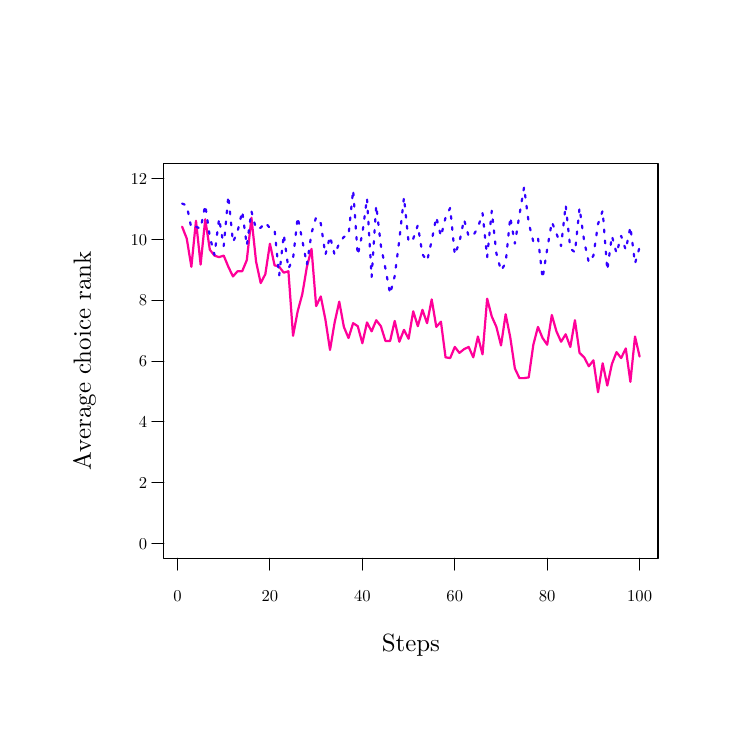
\begin{tikzpicture}[x=1pt,y=1pt]
\definecolor{fillColor}{RGB}{255,255,255}
\path[use as bounding box,fill=fillColor,fill opacity=0.00] (0,0) rectangle (252.94,252.94);
\begin{scope}
\path[clip] ( 49.20, 61.20) rectangle (227.75,203.75);
\definecolor{drawColor}{RGB}{255,0,153}

\path[draw=drawColor,line width= 0.8pt,line join=round,line cap=round] ( 55.81,181.03) --
	( 57.48,176.74) --
	( 59.15,166.54) --
	( 60.82,183.17) --
	( 62.49,167.35) --
	( 64.16,183.71) --
	( 65.83,172.71) --
	( 67.50,170.57) --
	( 69.17,170.03) --
	( 70.84,170.57) --
	( 72.51,166.54) --
	( 74.18,163.05) --
	( 75.85,164.93) --
	( 77.52,164.93) --
	( 79.19,168.96) --
	( 80.86,184.25) --
	( 82.53,168.42) --
	( 84.20,160.64) --
	( 85.87,163.86) --
	( 87.54,174.86) --
	( 89.21,167.08) --
	( 90.88,166.54) --
	( 92.55,164.40) --
	( 94.22,164.93) --
	( 95.89,141.59) --
	( 97.56,150.45) --
	( 99.23,156.62) --
	(100.90,166.54) --
	(102.57,172.98) --
	(104.24,152.32) --
	(105.91,155.81) --
	(107.58,147.50) --
	(109.25,136.50) --
	(110.92,146.42) --
	(112.59,153.93) --
	(114.26,144.81) --
	(115.93,140.79) --
	(117.60,146.15) --
	(119.27,145.08) --
	(120.94,138.91) --
	(122.61,146.42) --
	(124.28,143.20) --
	(125.95,147.23) --
	(127.62,145.08) --
	(129.29,139.72) --
	(130.96,139.72) --
	(132.63,146.96) --
	(134.30,139.45) --
	(135.97,143.74) --
	(137.64,140.52) --
	(139.31,150.45) --
	(140.98,145.08) --
	(142.65,150.98) --
	(144.32,146.15) --
	(145.99,154.74) --
	(147.66,144.81) --
	(149.33,146.69) --
	(151.00,133.81) --
	(152.67,133.55) --
	(154.34,137.57) --
	(156.01,135.42) --
	(157.68,136.76) --
	(159.35,137.57) --
	(161.02,133.81) --
	(162.69,141.33) --
	(164.36,134.89) --
	(166.03,155.01) --
	(167.70,148.57) --
	(169.37,144.81) --
	(171.04,138.11) --
	(172.71,149.37) --
	(174.38,141.06) --
	(176.05,129.79) --
	(177.71,126.30) --
	(179.38,126.30) --
	(181.05,126.57) --
	(182.72,138.37) --
	(184.39,144.81) --
	(186.06,140.79) --
	(187.73,138.37) --
	(189.40,149.10) --
	(191.07,143.20) --
	(192.74,139.45) --
	(194.41,142.13) --
	(196.08,137.57) --
	(197.75,147.23) --
	(199.42,135.42) --
	(201.09,133.81) --
	(202.76,130.59) --
	(204.43,132.74) --
	(206.10,121.21) --
	(207.77,131.67) --
	(209.44,123.62) --
	(211.11,131.40) --
	(212.78,135.69) --
	(214.45,133.55) --
	(216.12,137.03) --
	(217.79,124.96) --
	(219.46,141.33) --
	(221.13,134.08);
\end{scope}
\begin{scope}
\path[clip] (  0.00,  0.00) rectangle (252.94,252.94);
\definecolor{drawColor}{RGB}{0,0,0}

\path[draw=drawColor,line width= 0.4pt,line join=round,line cap=round] ( 54.14, 61.20) -- (221.13, 61.20);

\path[draw=drawColor,line width= 0.4pt,line join=round,line cap=round] ( 54.14, 61.20) -- ( 54.14, 56.92);

\path[draw=drawColor,line width= 0.4pt,line join=round,line cap=round] ( 87.54, 61.20) -- ( 87.54, 56.92);

\path[draw=drawColor,line width= 0.4pt,line join=round,line cap=round] (120.94, 61.20) -- (120.94, 56.92);

\path[draw=drawColor,line width= 0.4pt,line join=round,line cap=round] (154.34, 61.20) -- (154.34, 56.92);

\path[draw=drawColor,line width= 0.4pt,line join=round,line cap=round] (187.73, 61.20) -- (187.73, 56.92);

\path[draw=drawColor,line width= 0.4pt,line join=round,line cap=round] (221.13, 61.20) -- (221.13, 56.92);

\node[text=drawColor,anchor=base,inner sep=0pt, outer sep=0pt, scale=  0.60] at ( 54.14, 45.60) {0};

\node[text=drawColor,anchor=base,inner sep=0pt, outer sep=0pt, scale=  0.60] at ( 87.54, 45.60) {20};

\node[text=drawColor,anchor=base,inner sep=0pt, outer sep=0pt, scale=  0.60] at (120.94, 45.60) {40};

\node[text=drawColor,anchor=base,inner sep=0pt, outer sep=0pt, scale=  0.60] at (154.34, 45.60) {60};

\node[text=drawColor,anchor=base,inner sep=0pt, outer sep=0pt, scale=  0.60] at (187.73, 45.60) {80};

\node[text=drawColor,anchor=base,inner sep=0pt, outer sep=0pt, scale=  0.60] at (221.13, 45.60) {100};

\path[draw=drawColor,line width= 0.4pt,line join=round,line cap=round] ( 49.20, 66.48) -- ( 49.20,198.47);

\path[draw=drawColor,line width= 0.4pt,line join=round,line cap=round] ( 49.20, 66.48) -- ( 44.92, 66.48);

\path[draw=drawColor,line width= 0.4pt,line join=round,line cap=round] ( 49.20, 88.48) -- ( 44.92, 88.48);

\path[draw=drawColor,line width= 0.4pt,line join=round,line cap=round] ( 49.20,110.47) -- ( 44.92,110.47);

\path[draw=drawColor,line width= 0.4pt,line join=round,line cap=round] ( 49.20,132.47) -- ( 44.92,132.47);

\path[draw=drawColor,line width= 0.4pt,line join=round,line cap=round] ( 49.20,154.47) -- ( 44.92,154.47);

\path[draw=drawColor,line width= 0.4pt,line join=round,line cap=round] ( 49.20,176.47) -- ( 44.92,176.47);

\path[draw=drawColor,line width= 0.4pt,line join=round,line cap=round] ( 49.20,198.47) -- ( 44.92,198.47);

\node[text=drawColor,anchor=base east,inner sep=0pt, outer sep=0pt, scale=  0.60] at ( 43.20, 64.41) {0};

\node[text=drawColor,anchor=base east,inner sep=0pt, outer sep=0pt, scale=  0.60] at ( 43.20, 86.41) {2};

\node[text=drawColor,anchor=base east,inner sep=0pt, outer sep=0pt, scale=  0.60] at ( 43.20,108.41) {4};

\node[text=drawColor,anchor=base east,inner sep=0pt, outer sep=0pt, scale=  0.60] at ( 43.20,130.41) {6};

\node[text=drawColor,anchor=base east,inner sep=0pt, outer sep=0pt, scale=  0.60] at ( 43.20,152.40) {8};

\node[text=drawColor,anchor=base east,inner sep=0pt, outer sep=0pt, scale=  0.60] at ( 43.20,174.40) {10};

\node[text=drawColor,anchor=base east,inner sep=0pt, outer sep=0pt, scale=  0.60] at ( 43.20,196.40) {12};

\path[draw=drawColor,line width= 0.4pt,line join=round,line cap=round] ( 49.20, 61.20) --
	(227.75, 61.20) --
	(227.75,203.75) --
	( 49.20,203.75) --
	( 49.20, 61.20);
\end{scope}
\begin{scope}
\path[clip] (  0.00,  0.00) rectangle (252.94,252.94);
\definecolor{drawColor}{RGB}{0,0,0}

\node[text=drawColor,anchor=base,inner sep=0pt, outer sep=0pt, scale=  0.90] at (138.47, 27.60) {Steps};

\node[text=drawColor,rotate= 90.00,anchor=base,inner sep=0pt, outer sep=0pt, scale=  0.90] at ( 22.80,132.47) {Average choice rank};
\end{scope}
\begin{scope}
\path[clip] ( 49.20, 61.20) rectangle (227.75,203.75);
\definecolor{drawColor}{RGB}{51,0,255}

\path[draw=drawColor,line width= 0.8pt,dash pattern=on 1pt off 3pt ,line join=round,line cap=round] ( 55.81,189.39) --
	( 57.48,188.69) --
	( 59.15,180.48) --
	( 60.82,181.01) --
	( 62.49,180.31) --
	( 64.16,188.86) --
	( 65.83,177.34) --
	( 67.50,170.88) --
	( 69.17,183.98) --
	( 70.84,174.02) --
	( 72.51,192.18) --
	( 74.18,175.42) --
	( 75.85,179.26) --
	( 77.52,186.59) --
	( 79.19,174.20) --
	( 80.86,186.59) --
	( 82.53,180.13) --
	( 84.20,180.66) --
	( 85.87,182.58) --
	( 87.54,180.48) --
	( 89.21,179.96) --
	( 90.88,163.37) --
	( 92.55,178.21) --
	( 94.22,165.82) --
	( 95.89,169.48) --
	( 97.56,184.50) --
	( 99.23,176.12) --
	(100.90,167.39) --
	(102.57,178.74) --
	(104.24,184.50) --
	(105.91,182.23) --
	(107.58,170.88) --
	(109.25,177.52) --
	(110.92,170.88) --
	(112.59,175.07) --
	(114.26,177.34) --
	(115.93,177.86) --
	(117.60,194.28) --
	(119.27,170.71) --
	(120.94,178.56) --
	(122.61,191.31) --
	(124.28,162.85) --
	(125.95,188.69) --
	(127.62,174.20) --
	(129.29,165.82) --
	(130.96,156.74) --
	(132.63,163.20) --
	(134.30,176.29) --
	(135.97,191.66) --
	(137.64,175.42) --
	(139.31,176.64) --
	(140.98,181.53) --
	(142.65,171.06) --
	(144.32,168.61) --
	(145.99,175.94) --
	(147.66,184.50) --
	(149.33,177.52) --
	(151.00,184.32) --
	(152.67,187.82) --
	(154.34,170.88) --
	(156.01,175.42) --
	(157.68,183.63) --
	(159.35,177.52) --
	(161.02,177.86) --
	(162.69,180.66) --
	(164.36,185.90) --
	(166.03,170.01) --
	(167.70,186.77) --
	(169.37,171.40) --
	(171.04,165.12) --
	(172.71,167.91) --
	(174.38,184.50) --
	(176.05,174.90) --
	(177.71,185.37) --
	(179.38,195.32) --
	(181.05,182.40) --
	(182.72,175.59) --
	(184.39,177.17) --
	(186.06,162.33) --
	(187.73,172.98) --
	(189.40,182.75) --
	(191.07,178.56) --
	(192.74,174.02) --
	(194.41,188.86) --
	(196.08,173.15) --
	(197.75,171.75) --
	(199.42,187.82) --
	(201.09,175.77) --
	(202.76,168.09) --
	(204.43,170.53) --
	(206.10,182.05) --
	(207.77,186.77) --
	(209.44,165.29) --
	(211.11,177.69) --
	(212.78,171.40) --
	(214.45,177.69) --
	(216.12,172.63) --
	(217.79,181.01) --
	(219.46,167.74) --
	(221.13,173.67);
\end{scope}
\end{tikzpicture}
 \\
		(\textbf{a}) Blockwise entropy by cluster & (\textbf{b}) Average choice rank by cluster \\
	\end{tabular} \quad
	\caption{Clustering on choices vs. model parameter estimation (top sub figures: experiment 1, high noise, bottom: experiment 1, low noise)}
	\label{fig:cluse1c3}
\end{figure}


\begin{figure}[H]
	\centering
	\small
	\hspace*{-0.7in}
	\begin{tabular}{cc}
			% Created by tikzDevice version 0.10.1 on 2016-06-30 12:20:31
% !TEX encoding = UTF-8 Unicode
\begin{tikzpicture}[x=1pt,y=1pt]
\definecolor{fillColor}{RGB}{255,255,255}
\path[use as bounding box,fill=fillColor,fill opacity=0.00] (0,0) rectangle (252.94,252.94);
\begin{scope}
\path[clip] ( 49.20, 61.20) rectangle (227.75,203.75);
\definecolor{drawColor}{RGB}{255,0,153}

\path[draw=drawColor,line width= 0.8pt,line join=round,line cap=round] ( 58.54,142.17) -- ( 71.46,116.80);

\path[draw=drawColor,line width= 0.8pt,line join=round,line cap=round] ( 77.70,106.60) -- ( 89.04, 90.90);

\path[draw=drawColor,line width= 0.8pt,line join=round,line cap=round] ( 97.39, 89.58) -- (106.08, 95.97);

\path[draw=drawColor,line width= 0.8pt,line join=round,line cap=round] (116.92, 99.43) -- (123.29, 99.33);

\path[draw=drawColor,line width= 0.8pt,line join=round,line cap=round] (133.71, 95.18) -- (143.24, 86.44);

\path[draw=drawColor,line width= 0.8pt,line join=round,line cap=round] (153.61, 81.63) -- (160.07, 80.83);

\path[draw=drawColor,line width= 0.8pt,line join=round,line cap=round] (171.88, 81.41) -- (178.54, 82.93);

\path[draw=drawColor,line width= 0.8pt,line join=round,line cap=round] (189.70, 81.46) -- (197.46, 77.37);

\path[draw=drawColor,line width= 0.8pt,line join=round,line cap=round] (208.74, 74.10) -- (215.15, 73.58);
\definecolor{fillColor}{RGB}{255,0,153}

\path[fill=fillColor] ( 55.81,147.51) circle (  1.35);

\path[fill=fillColor] ( 74.18,111.46) circle (  1.35);

\path[fill=fillColor] ( 92.55, 86.03) circle (  1.35);

\path[fill=fillColor] (110.92, 99.52) circle (  1.35);

\path[fill=fillColor] (129.29, 99.24) circle (  1.35);

\path[fill=fillColor] (147.66, 82.38) circle (  1.35);

\path[fill=fillColor] (166.03, 80.08) circle (  1.35);

\path[fill=fillColor] (184.39, 84.26) circle (  1.35);

\path[fill=fillColor] (202.76, 74.58) circle (  1.35);

\path[fill=fillColor] (221.13, 73.10) circle (  1.35);
\end{scope}
\begin{scope}
\path[clip] (  0.00,  0.00) rectangle (252.94,252.94);
\definecolor{drawColor}{RGB}{0,0,0}

\path[draw=drawColor,line width= 0.4pt,line join=round,line cap=round] ( 74.18, 61.20) -- (221.13, 61.20);

\path[draw=drawColor,line width= 0.4pt,line join=round,line cap=round] ( 74.18, 61.20) -- ( 74.18, 56.92);

\path[draw=drawColor,line width= 0.4pt,line join=round,line cap=round] (110.92, 61.20) -- (110.92, 56.92);

\path[draw=drawColor,line width= 0.4pt,line join=round,line cap=round] (147.66, 61.20) -- (147.66, 56.92);

\path[draw=drawColor,line width= 0.4pt,line join=round,line cap=round] (184.39, 61.20) -- (184.39, 56.92);

\path[draw=drawColor,line width= 0.4pt,line join=round,line cap=round] (221.13, 61.20) -- (221.13, 56.92);

\node[text=drawColor,anchor=base,inner sep=0pt, outer sep=0pt, scale=  0.60] at ( 74.18, 45.60) {2};

\node[text=drawColor,anchor=base,inner sep=0pt, outer sep=0pt, scale=  0.60] at (110.92, 45.60) {4};

\node[text=drawColor,anchor=base,inner sep=0pt, outer sep=0pt, scale=  0.60] at (147.66, 45.60) {6};

\node[text=drawColor,anchor=base,inner sep=0pt, outer sep=0pt, scale=  0.60] at (184.39, 45.60) {8};

\node[text=drawColor,anchor=base,inner sep=0pt, outer sep=0pt, scale=  0.60] at (221.13, 45.60) {10};

\path[draw=drawColor,line width= 0.4pt,line join=round,line cap=round] ( 49.20, 66.48) -- ( 49.20,198.47);

\path[draw=drawColor,line width= 0.4pt,line join=round,line cap=round] ( 49.20, 66.48) -- ( 44.92, 66.48);

\path[draw=drawColor,line width= 0.4pt,line join=round,line cap=round] ( 49.20, 85.33) -- ( 44.92, 85.33);

\path[draw=drawColor,line width= 0.4pt,line join=round,line cap=round] ( 49.20,104.19) -- ( 44.92,104.19);

\path[draw=drawColor,line width= 0.4pt,line join=round,line cap=round] ( 49.20,123.04) -- ( 44.92,123.04);

\path[draw=drawColor,line width= 0.4pt,line join=round,line cap=round] ( 49.20,141.90) -- ( 44.92,141.90);

\path[draw=drawColor,line width= 0.4pt,line join=round,line cap=round] ( 49.20,160.76) -- ( 44.92,160.76);

\path[draw=drawColor,line width= 0.4pt,line join=round,line cap=round] ( 49.20,179.61) -- ( 44.92,179.61);

\path[draw=drawColor,line width= 0.4pt,line join=round,line cap=round] ( 49.20,198.47) -- ( 44.92,198.47);

\node[text=drawColor,anchor=base east,inner sep=0pt, outer sep=0pt, scale=  0.60] at ( 43.20, 64.41) {0.0};

\node[text=drawColor,anchor=base east,inner sep=0pt, outer sep=0pt, scale=  0.60] at ( 43.20, 83.27) {0.5};

\node[text=drawColor,anchor=base east,inner sep=0pt, outer sep=0pt, scale=  0.60] at ( 43.20,102.12) {1.0};

\node[text=drawColor,anchor=base east,inner sep=0pt, outer sep=0pt, scale=  0.60] at ( 43.20,120.98) {1.5};

\node[text=drawColor,anchor=base east,inner sep=0pt, outer sep=0pt, scale=  0.60] at ( 43.20,139.83) {2.0};

\node[text=drawColor,anchor=base east,inner sep=0pt, outer sep=0pt, scale=  0.60] at ( 43.20,158.69) {2.5};

\node[text=drawColor,anchor=base east,inner sep=0pt, outer sep=0pt, scale=  0.60] at ( 43.20,177.54) {3.0};

\node[text=drawColor,anchor=base east,inner sep=0pt, outer sep=0pt, scale=  0.60] at ( 43.20,196.40) {3.5};

\path[draw=drawColor,line width= 0.4pt,line join=round,line cap=round] ( 49.20, 61.20) --
	(227.75, 61.20) --
	(227.75,203.75) --
	( 49.20,203.75) --
	( 49.20, 61.20);
\end{scope}
\begin{scope}
\path[clip] (  0.00,  0.00) rectangle (252.94,252.94);
\definecolor{drawColor}{RGB}{0,0,0}

\node[text=drawColor,anchor=base,inner sep=0pt, outer sep=0pt, scale=  0.90] at (138.47, 27.60) {Steps};

\node[text=drawColor,rotate= 90.00,anchor=base,inner sep=0pt, outer sep=0pt, scale=  0.90] at ( 22.80,132.47) {Avergage entropy accross groups};
\end{scope}
\begin{scope}
\path[clip] ( 49.20, 61.20) rectangle (227.75,203.75);
\definecolor{drawColor}{RGB}{51,0,255}

\path[draw=drawColor,line width= 0.8pt,line join=round,line cap=round] ( 61.40,176.84) -- ( 68.59,174.04);

\path[draw=drawColor,line width= 0.8pt,line join=round,line cap=round] ( 78.20,167.41) -- ( 88.54,155.92);

\path[draw=drawColor,line width= 0.8pt,line join=round,line cap=round] ( 97.72,148.43) -- (105.75,143.72);

\path[draw=drawColor,line width= 0.8pt,line join=round,line cap=round] (115.71,137.07) -- (124.49,130.47);

\path[draw=drawColor,line width= 0.8pt,line join=round,line cap=round] (135.29,126.84) -- (141.66,126.82);

\path[draw=drawColor,line width= 0.8pt,line join=round,line cap=round] (152.80,123.71) -- (160.88,118.88);

\path[draw=drawColor,line width= 0.8pt,line join=round,line cap=round] (171.95,114.82) -- (178.47,113.74);

\path[draw=drawColor,line width= 0.8pt,line join=round,line cap=round] (189.77,110.10) -- (197.39,106.34);

\path[draw=drawColor,line width= 0.8pt,line join=round,line cap=round] (208.63,104.95) -- (215.27,106.38);

\path[draw=drawColor,line width= 0.8pt,line join=round,line cap=round] ( 54.46,177.66) -- ( 57.16,180.36);

\path[draw=drawColor,line width= 0.8pt,line join=round,line cap=round] ( 54.46,180.36) -- ( 57.16,177.66);

\path[draw=drawColor,line width= 0.8pt,line join=round,line cap=round] ( 53.90,179.01) -- ( 57.72,179.01);

\path[draw=drawColor,line width= 0.8pt,line join=round,line cap=round] ( 55.81,177.10) -- ( 55.81,180.92);

\path[draw=drawColor,line width= 0.8pt,line join=round,line cap=round] ( 72.83,170.52) -- ( 75.53,173.22);

\path[draw=drawColor,line width= 0.8pt,line join=round,line cap=round] ( 72.83,173.22) -- ( 75.53,170.52);

\path[draw=drawColor,line width= 0.8pt,line join=round,line cap=round] ( 72.27,171.87) -- ( 76.09,171.87);

\path[draw=drawColor,line width= 0.8pt,line join=round,line cap=round] ( 74.18,169.96) -- ( 74.18,173.78);

\path[draw=drawColor,line width= 0.8pt,line join=round,line cap=round] ( 91.20,150.11) -- ( 93.90,152.81);

\path[draw=drawColor,line width= 0.8pt,line join=round,line cap=round] ( 91.20,152.81) -- ( 93.90,150.11);

\path[draw=drawColor,line width= 0.8pt,line join=round,line cap=round] ( 90.64,151.46) -- ( 94.46,151.46);

\path[draw=drawColor,line width= 0.8pt,line join=round,line cap=round] ( 92.55,149.56) -- ( 92.55,153.37);

\path[draw=drawColor,line width= 0.8pt,line join=round,line cap=round] (109.57,139.33) -- (112.27,142.03);

\path[draw=drawColor,line width= 0.8pt,line join=round,line cap=round] (109.57,142.03) -- (112.27,139.33);

\path[draw=drawColor,line width= 0.8pt,line join=round,line cap=round] (109.01,140.68) -- (112.83,140.68);

\path[draw=drawColor,line width= 0.8pt,line join=round,line cap=round] (110.92,138.77) -- (110.92,142.59);

\path[draw=drawColor,line width= 0.8pt,line join=round,line cap=round] (127.94,125.51) -- (130.64,128.21);

\path[draw=drawColor,line width= 0.8pt,line join=round,line cap=round] (127.94,128.21) -- (130.64,125.51);

\path[draw=drawColor,line width= 0.8pt,line join=round,line cap=round] (127.38,126.86) -- (131.20,126.86);

\path[draw=drawColor,line width= 0.8pt,line join=round,line cap=round] (129.29,124.95) -- (129.29,128.77);

\path[draw=drawColor,line width= 0.8pt,line join=round,line cap=round] (146.31,125.45) -- (149.01,128.15);

\path[draw=drawColor,line width= 0.8pt,line join=round,line cap=round] (146.31,128.15) -- (149.01,125.45);

\path[draw=drawColor,line width= 0.8pt,line join=round,line cap=round] (145.75,126.80) -- (149.57,126.80);

\path[draw=drawColor,line width= 0.8pt,line join=round,line cap=round] (147.66,124.89) -- (147.66,128.71);

\path[draw=drawColor,line width= 0.8pt,line join=round,line cap=round] (164.68,114.44) -- (167.38,117.14);

\path[draw=drawColor,line width= 0.8pt,line join=round,line cap=round] (164.68,117.14) -- (167.38,114.44);

\path[draw=drawColor,line width= 0.8pt,line join=round,line cap=round] (164.12,115.79) -- (167.93,115.79);

\path[draw=drawColor,line width= 0.8pt,line join=round,line cap=round] (166.03,113.89) -- (166.03,117.70);

\path[draw=drawColor,line width= 0.8pt,line join=round,line cap=round] (183.04,111.41) -- (185.74,114.11);

\path[draw=drawColor,line width= 0.8pt,line join=round,line cap=round] (183.04,114.11) -- (185.74,111.41);

\path[draw=drawColor,line width= 0.8pt,line join=round,line cap=round] (182.49,112.76) -- (186.30,112.76);

\path[draw=drawColor,line width= 0.8pt,line join=round,line cap=round] (184.39,110.85) -- (184.39,114.67);

\path[draw=drawColor,line width= 0.8pt,line join=round,line cap=round] (201.41,102.33) -- (204.11,105.03);

\path[draw=drawColor,line width= 0.8pt,line join=round,line cap=round] (201.41,105.03) -- (204.11,102.33);

\path[draw=drawColor,line width= 0.8pt,line join=round,line cap=round] (200.85,103.68) -- (204.67,103.68);

\path[draw=drawColor,line width= 0.8pt,line join=round,line cap=round] (202.76,101.77) -- (202.76,105.59);

\path[draw=drawColor,line width= 0.8pt,line join=round,line cap=round] (219.78,106.30) -- (222.48,109.00);

\path[draw=drawColor,line width= 0.8pt,line join=round,line cap=round] (219.78,109.00) -- (222.48,106.30);

\path[draw=drawColor,line width= 0.8pt,line join=round,line cap=round] (219.22,107.65) -- (223.04,107.65);

\path[draw=drawColor,line width= 0.8pt,line join=round,line cap=round] (221.13,105.74) -- (221.13,109.56);
\definecolor{drawColor}{RGB}{255,0,153}

\path[draw=drawColor,line width= 0.4pt,line join=round,line cap=round] ( 50.82, 72.00) -- ( 61.62, 72.00);

\path[draw=drawColor,line width= 0.4pt,line join=round,line cap=round] ( 56.22, 72.00) circle (  1.35);
\definecolor{drawColor}{RGB}{0,0,0}

\node[text=drawColor,anchor=base west,inner sep=0pt, outer sep=0pt, scale=  0.60] at ( 67.02, 69.93) {First Cluster};

\node[text=drawColor,anchor=base west,inner sep=0pt, outer sep=0pt, scale=  0.60] at (124.21, 69.93) {Second Cluster};
\end{scope}
\end{tikzpicture}
 & % Created by tikzDevice version 0.10.1 on 2016-06-30 12:15:51
% !TEX encoding = UTF-8 Unicode
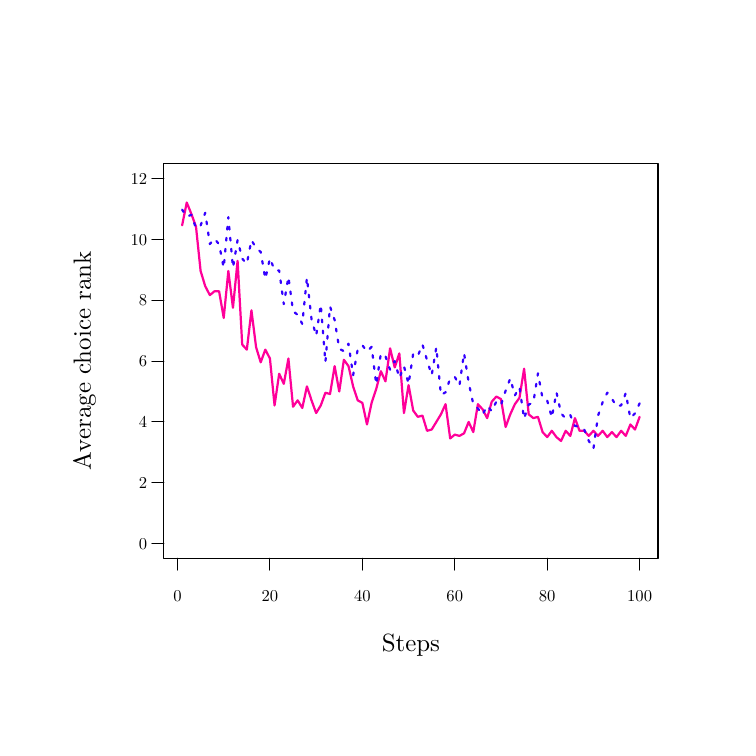
\begin{tikzpicture}[x=1pt,y=1pt]
\definecolor{fillColor}{RGB}{255,255,255}
\path[use as bounding box,fill=fillColor,fill opacity=0.00] (0,0) rectangle (252.94,252.94);
\begin{scope}
\path[clip] ( 49.20, 61.20) rectangle (227.75,203.75);
\definecolor{drawColor}{RGB}{255,0,153}

\path[draw=drawColor,line width= 0.8pt,line join=round,line cap=round] ( 55.81,181.51) --
	( 57.48,189.76) --
	( 59.15,185.63) --
	( 60.82,181.05) --
	( 62.49,165.01) --
	( 64.16,159.51) --
	( 65.83,156.30) --
	( 67.50,157.68) --
	( 69.17,157.68) --
	( 70.84,148.05) --
	( 72.51,165.01) --
	( 74.18,151.72) --
	( 75.85,168.68) --
	( 77.52,138.43) --
	( 79.19,136.60) --
	( 80.86,150.80) --
	( 82.53,137.51) --
	( 84.20,132.01) --
	( 85.87,136.60) --
	( 87.54,133.39) --
	( 89.21,116.43) --
	( 90.88,127.89) --
	( 92.55,124.22) --
	( 94.22,133.39) --
	( 95.89,115.97) --
	( 97.56,118.27) --
	( 99.23,115.52) --
	(100.90,123.31) --
	(102.57,118.27) --
	(104.24,113.68) --
	(105.91,116.43) --
	(107.58,121.02) --
	(109.25,120.56) --
	(110.92,130.64) --
	(112.59,121.47) --
	(114.26,132.93) --
	(115.93,130.64) --
	(117.60,123.31) --
	(119.27,118.27) --
	(120.94,117.35) --
	(122.61,109.56) --
	(124.28,117.35) --
	(125.95,122.39) --
	(127.62,128.81) --
	(129.29,125.14) --
	(130.96,137.06) --
	(132.63,130.18) --
	(134.30,135.22) --
	(135.97,113.68) --
	(137.64,123.77) --
	(139.31,114.60) --
	(140.98,112.31) --
	(142.65,112.77) --
	(144.32,107.27) --
	(145.99,107.73) --
	(147.66,110.47) --
	(149.33,113.22) --
	(151.00,116.89) --
	(152.67,104.52) --
	(154.34,105.89) --
	(156.01,105.43) --
	(157.68,106.35) --
	(159.35,110.47) --
	(161.02,106.81) --
	(162.69,116.89) --
	(164.36,115.06) --
	(166.03,111.85) --
	(167.70,117.81) --
	(169.37,119.64) --
	(171.04,118.72) --
	(172.71,108.64) --
	(174.38,113.22) --
	(176.05,116.89) --
	(177.71,119.18) --
	(179.38,129.72) --
	(181.05,113.22) --
	(182.72,111.85) --
	(184.39,112.31) --
	(186.06,106.81) --
	(187.73,104.98) --
	(189.40,107.27) --
	(191.07,104.98) --
	(192.74,103.60) --
	(194.41,107.27) --
	(196.08,105.43) --
	(197.75,111.85) --
	(199.42,107.27) --
	(201.09,107.27) --
	(202.76,105.43) --
	(204.43,107.27) --
	(206.10,105.43) --
	(207.77,107.27) --
	(209.44,104.98) --
	(211.11,106.81) --
	(212.78,104.98) --
	(214.45,107.27) --
	(216.12,105.43) --
	(217.79,109.56) --
	(219.46,107.73) --
	(221.13,112.31);
\end{scope}
\begin{scope}
\path[clip] (  0.00,  0.00) rectangle (252.94,252.94);
\definecolor{drawColor}{RGB}{0,0,0}

\path[draw=drawColor,line width= 0.4pt,line join=round,line cap=round] ( 54.14, 61.20) -- (221.13, 61.20);

\path[draw=drawColor,line width= 0.4pt,line join=round,line cap=round] ( 54.14, 61.20) -- ( 54.14, 56.92);

\path[draw=drawColor,line width= 0.4pt,line join=round,line cap=round] ( 87.54, 61.20) -- ( 87.54, 56.92);

\path[draw=drawColor,line width= 0.4pt,line join=round,line cap=round] (120.94, 61.20) -- (120.94, 56.92);

\path[draw=drawColor,line width= 0.4pt,line join=round,line cap=round] (154.34, 61.20) -- (154.34, 56.92);

\path[draw=drawColor,line width= 0.4pt,line join=round,line cap=round] (187.73, 61.20) -- (187.73, 56.92);

\path[draw=drawColor,line width= 0.4pt,line join=round,line cap=round] (221.13, 61.20) -- (221.13, 56.92);

\node[text=drawColor,anchor=base,inner sep=0pt, outer sep=0pt, scale=  0.60] at ( 54.14, 45.60) {0};

\node[text=drawColor,anchor=base,inner sep=0pt, outer sep=0pt, scale=  0.60] at ( 87.54, 45.60) {20};

\node[text=drawColor,anchor=base,inner sep=0pt, outer sep=0pt, scale=  0.60] at (120.94, 45.60) {40};

\node[text=drawColor,anchor=base,inner sep=0pt, outer sep=0pt, scale=  0.60] at (154.34, 45.60) {60};

\node[text=drawColor,anchor=base,inner sep=0pt, outer sep=0pt, scale=  0.60] at (187.73, 45.60) {80};

\node[text=drawColor,anchor=base,inner sep=0pt, outer sep=0pt, scale=  0.60] at (221.13, 45.60) {100};

\path[draw=drawColor,line width= 0.4pt,line join=round,line cap=round] ( 49.20, 66.48) -- ( 49.20,198.47);

\path[draw=drawColor,line width= 0.4pt,line join=round,line cap=round] ( 49.20, 66.48) -- ( 44.92, 66.48);

\path[draw=drawColor,line width= 0.4pt,line join=round,line cap=round] ( 49.20, 88.48) -- ( 44.92, 88.48);

\path[draw=drawColor,line width= 0.4pt,line join=round,line cap=round] ( 49.20,110.47) -- ( 44.92,110.47);

\path[draw=drawColor,line width= 0.4pt,line join=round,line cap=round] ( 49.20,132.47) -- ( 44.92,132.47);

\path[draw=drawColor,line width= 0.4pt,line join=round,line cap=round] ( 49.20,154.47) -- ( 44.92,154.47);

\path[draw=drawColor,line width= 0.4pt,line join=round,line cap=round] ( 49.20,176.47) -- ( 44.92,176.47);

\path[draw=drawColor,line width= 0.4pt,line join=round,line cap=round] ( 49.20,198.47) -- ( 44.92,198.47);

\node[text=drawColor,anchor=base east,inner sep=0pt, outer sep=0pt, scale=  0.60] at ( 43.20, 64.41) {0};

\node[text=drawColor,anchor=base east,inner sep=0pt, outer sep=0pt, scale=  0.60] at ( 43.20, 86.41) {2};

\node[text=drawColor,anchor=base east,inner sep=0pt, outer sep=0pt, scale=  0.60] at ( 43.20,108.41) {4};

\node[text=drawColor,anchor=base east,inner sep=0pt, outer sep=0pt, scale=  0.60] at ( 43.20,130.41) {6};

\node[text=drawColor,anchor=base east,inner sep=0pt, outer sep=0pt, scale=  0.60] at ( 43.20,152.40) {8};

\node[text=drawColor,anchor=base east,inner sep=0pt, outer sep=0pt, scale=  0.60] at ( 43.20,174.40) {10};

\node[text=drawColor,anchor=base east,inner sep=0pt, outer sep=0pt, scale=  0.60] at ( 43.20,196.40) {12};

\path[draw=drawColor,line width= 0.4pt,line join=round,line cap=round] ( 49.20, 61.20) --
	(227.75, 61.20) --
	(227.75,203.75) --
	( 49.20,203.75) --
	( 49.20, 61.20);
\end{scope}
\begin{scope}
\path[clip] (  0.00,  0.00) rectangle (252.94,252.94);
\definecolor{drawColor}{RGB}{0,0,0}

\node[text=drawColor,anchor=base,inner sep=0pt, outer sep=0pt, scale=  0.90] at (138.47, 27.60) {Steps};

\node[text=drawColor,rotate= 90.00,anchor=base,inner sep=0pt, outer sep=0pt, scale=  0.90] at ( 22.80,132.47) {Average choice rank};
\end{scope}
\begin{scope}
\path[clip] ( 49.20, 61.20) rectangle (227.75,203.75);
\definecolor{drawColor}{RGB}{51,0,255}

\path[draw=drawColor,line width= 0.8pt,dash pattern=on 1pt off 3pt ,line join=round,line cap=round] ( 55.81,187.18) --
	( 57.48,184.61) --
	( 59.15,185.32) --
	( 60.82,180.47) --
	( 62.49,181.47) --
	( 64.16,186.04) --
	( 65.83,174.75) --
	( 67.50,176.75) --
	( 69.17,174.61) --
	( 70.84,166.18) --
	( 72.51,184.47) --
	( 74.18,166.18) --
	( 75.85,176.18) --
	( 77.52,169.47) --
	( 79.19,167.61) --
	( 80.86,176.18) --
	( 82.53,173.33) --
	( 84.20,171.90) --
	( 85.87,162.18) --
	( 87.54,169.61) --
	( 89.21,165.33) --
	( 90.88,165.18) --
	( 92.55,153.04) --
	( 94.22,162.90) --
	( 95.89,150.47) --
	( 97.56,149.19) --
	( 99.23,145.90) --
	(100.90,162.61) --
	(102.57,147.61) --
	(104.24,141.61) --
	(105.91,152.90) --
	(107.58,132.04) --
	(109.25,152.18) --
	(110.92,147.33) --
	(112.59,136.90) --
	(114.26,136.04) --
	(115.93,138.76) --
	(117.60,127.33) --
	(119.27,136.76) --
	(120.94,138.19) --
	(122.61,135.90) --
	(124.28,137.61) --
	(125.95,124.04) --
	(127.62,135.19) --
	(129.29,134.19) --
	(130.96,129.33) --
	(132.63,132.47) --
	(134.30,126.33) --
	(135.97,130.62) --
	(137.64,124.19) --
	(139.31,135.19) --
	(140.98,134.33) --
	(142.65,138.47) --
	(144.32,132.76) --
	(145.99,127.33) --
	(147.66,137.47) --
	(149.33,120.19) --
	(151.00,121.19) --
	(152.67,126.19) --
	(154.34,126.76) --
	(156.01,123.62) --
	(157.68,135.33) --
	(159.35,124.76) --
	(161.02,116.90) --
	(162.69,115.33) --
	(164.36,113.05) --
	(166.03,116.33) --
	(167.70,114.33) --
	(169.37,117.90) --
	(171.04,116.62) --
	(172.71,121.76) --
	(174.38,126.19) --
	(176.05,120.05) --
	(177.71,123.04) --
	(179.38,111.62) --
	(181.05,116.76) --
	(182.72,117.47) --
	(184.39,128.04) --
	(186.06,118.90) --
	(187.73,118.19) --
	(189.40,112.05) --
	(191.07,121.19) --
	(192.74,113.62) --
	(194.41,111.62) --
	(196.08,112.90) --
	(197.75,109.05) --
	(199.42,108.76) --
	(201.09,107.76) --
	(202.76,103.62) --
	(204.43,100.76) --
	(206.10,112.76) --
	(207.77,117.62) --
	(209.44,121.05) --
	(211.11,118.90) --
	(212.78,116.05) --
	(214.45,116.47) --
	(216.12,120.90) --
	(217.79,111.76) --
	(219.46,113.62) --
	(221.13,117.19);
\end{scope}
\end{tikzpicture}
 \\
				(\textbf{a}) Blockwise entropy by cluster & (\textbf{b}) Average choice rank by cluster \\
			% Created by tikzDevice version 0.10.1 on 2016-06-30 12:57:10
% !TEX encoding = UTF-8 Unicode
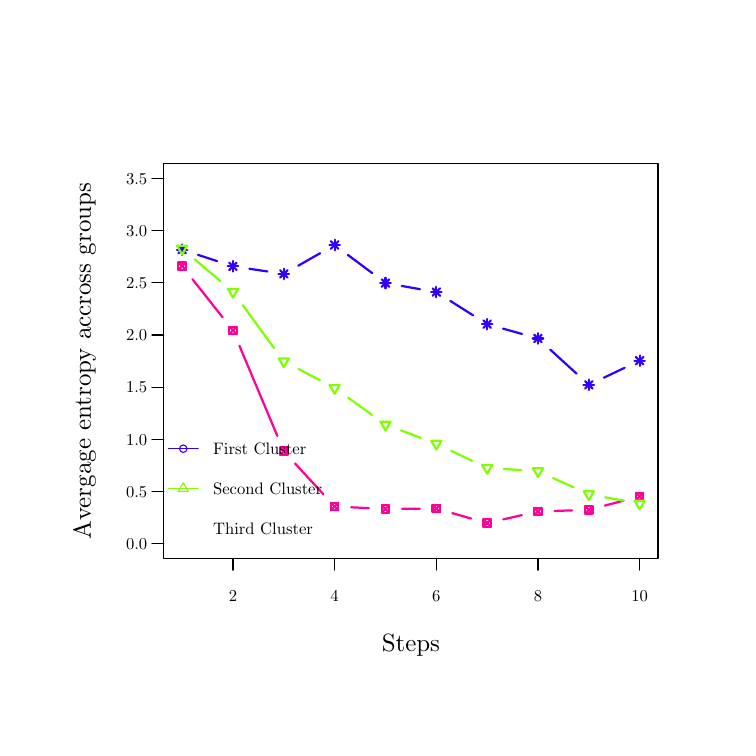
\begin{tikzpicture}[x=1pt,y=1pt]
\definecolor{fillColor}{RGB}{255,255,255}
\path[use as bounding box,fill=fillColor,fill opacity=0.00] (0,0) rectangle (252.94,252.94);
\begin{scope}
\path[clip] ( 49.20, 61.20) rectangle (227.75,203.75);
\definecolor{drawColor}{RGB}{51,0,255}

\path[draw=drawColor,line width= 0.8pt,line join=round,line cap=round] ( 61.52,170.85) -- ( 68.48,168.58);

\path[draw=drawColor,line width= 0.8pt,line join=round,line cap=round] ( 80.12,165.82) -- ( 86.62,164.85);

\path[draw=drawColor,line width= 0.8pt,line join=round,line cap=round] ( 97.77,166.93) -- (105.70,171.44);

\path[draw=drawColor,line width= 0.8pt,line join=round,line cap=round] (115.72,170.81) -- (124.48,164.26);

\path[draw=drawColor,line width= 0.8pt,line join=round,line cap=round] (135.19,159.61) -- (141.75,158.44);

\path[draw=drawColor,line width= 0.8pt,line join=round,line cap=round] (152.73,154.19) -- (160.95,149.00);

\path[draw=drawColor,line width= 0.8pt,line join=round,line cap=round] (171.80,144.18) -- (178.62,142.27);

\path[draw=drawColor,line width= 0.8pt,line join=round,line cap=round] (188.83,136.60) -- (198.33,127.92);

\path[draw=drawColor,line width= 0.8pt,line join=round,line cap=round] (208.18,126.45) -- (215.71,130.02);

\path[draw=drawColor,line width= 0.8pt,line join=round,line cap=round] ( 54.46,171.37) -- ( 57.16,174.07);

\path[draw=drawColor,line width= 0.8pt,line join=round,line cap=round] ( 54.46,174.07) -- ( 57.16,171.37);

\path[draw=drawColor,line width= 0.8pt,line join=round,line cap=round] ( 53.90,172.72) -- ( 57.72,172.72);

\path[draw=drawColor,line width= 0.8pt,line join=round,line cap=round] ( 55.81,170.81) -- ( 55.81,174.63);

\path[draw=drawColor,line width= 0.8pt,line join=round,line cap=round] ( 72.83,165.36) -- ( 75.53,168.06);

\path[draw=drawColor,line width= 0.8pt,line join=round,line cap=round] ( 72.83,168.06) -- ( 75.53,165.36);

\path[draw=drawColor,line width= 0.8pt,line join=round,line cap=round] ( 72.27,166.71) -- ( 76.09,166.71);

\path[draw=drawColor,line width= 0.8pt,line join=round,line cap=round] ( 74.18,164.80) -- ( 74.18,168.62);

\path[draw=drawColor,line width= 0.8pt,line join=round,line cap=round] ( 91.20,162.61) -- ( 93.90,165.31);

\path[draw=drawColor,line width= 0.8pt,line join=round,line cap=round] ( 91.20,165.31) -- ( 93.90,162.61);

\path[draw=drawColor,line width= 0.8pt,line join=round,line cap=round] ( 90.64,163.96) -- ( 94.46,163.96);

\path[draw=drawColor,line width= 0.8pt,line join=round,line cap=round] ( 92.55,162.05) -- ( 92.55,165.87);

\path[draw=drawColor,line width= 0.8pt,line join=round,line cap=round] (109.57,173.05) -- (112.27,175.75);

\path[draw=drawColor,line width= 0.8pt,line join=round,line cap=round] (109.57,175.75) -- (112.27,173.05);

\path[draw=drawColor,line width= 0.8pt,line join=round,line cap=round] (109.01,174.40) -- (112.83,174.40);

\path[draw=drawColor,line width= 0.8pt,line join=round,line cap=round] (110.92,172.49) -- (110.92,176.31);

\path[draw=drawColor,line width= 0.8pt,line join=round,line cap=round] (127.94,159.31) -- (130.64,162.01);

\path[draw=drawColor,line width= 0.8pt,line join=round,line cap=round] (127.94,162.01) -- (130.64,159.31);

\path[draw=drawColor,line width= 0.8pt,line join=round,line cap=round] (127.38,160.66) -- (131.20,160.66);

\path[draw=drawColor,line width= 0.8pt,line join=round,line cap=round] (129.29,158.75) -- (129.29,162.57);

\path[draw=drawColor,line width= 0.8pt,line join=round,line cap=round] (146.31,156.04) -- (149.01,158.74);

\path[draw=drawColor,line width= 0.8pt,line join=round,line cap=round] (146.31,158.74) -- (149.01,156.04);

\path[draw=drawColor,line width= 0.8pt,line join=round,line cap=round] (145.75,157.39) -- (149.57,157.39);

\path[draw=drawColor,line width= 0.8pt,line join=round,line cap=round] (147.66,155.48) -- (147.66,159.30);

\path[draw=drawColor,line width= 0.8pt,line join=round,line cap=round] (164.68,144.45) -- (167.38,147.15);

\path[draw=drawColor,line width= 0.8pt,line join=round,line cap=round] (164.68,147.15) -- (167.38,144.45);

\path[draw=drawColor,line width= 0.8pt,line join=round,line cap=round] (164.12,145.80) -- (167.93,145.80);

\path[draw=drawColor,line width= 0.8pt,line join=round,line cap=round] (166.03,143.89) -- (166.03,147.71);

\path[draw=drawColor,line width= 0.8pt,line join=round,line cap=round] (183.04,139.30) -- (185.74,142.00);

\path[draw=drawColor,line width= 0.8pt,line join=round,line cap=round] (183.04,142.00) -- (185.74,139.30);

\path[draw=drawColor,line width= 0.8pt,line join=round,line cap=round] (182.49,140.65) -- (186.30,140.65);

\path[draw=drawColor,line width= 0.8pt,line join=round,line cap=round] (184.39,138.74) -- (184.39,142.56);

\path[draw=drawColor,line width= 0.8pt,line join=round,line cap=round] (201.41,122.52) -- (204.11,125.22);

\path[draw=drawColor,line width= 0.8pt,line join=round,line cap=round] (201.41,125.22) -- (204.11,122.52);

\path[draw=drawColor,line width= 0.8pt,line join=round,line cap=round] (200.85,123.87) -- (204.67,123.87);

\path[draw=drawColor,line width= 0.8pt,line join=round,line cap=round] (202.76,121.97) -- (202.76,125.78);

\path[draw=drawColor,line width= 0.8pt,line join=round,line cap=round] (219.78,131.24) -- (222.48,133.94);

\path[draw=drawColor,line width= 0.8pt,line join=round,line cap=round] (219.78,133.94) -- (222.48,131.24);

\path[draw=drawColor,line width= 0.8pt,line join=round,line cap=round] (219.22,132.59) -- (223.04,132.59);

\path[draw=drawColor,line width= 0.8pt,line join=round,line cap=round] (221.13,130.69) -- (221.13,134.50);
\end{scope}
\begin{scope}
\path[clip] (  0.00,  0.00) rectangle (252.94,252.94);
\definecolor{drawColor}{RGB}{0,0,0}

\path[draw=drawColor,line width= 0.4pt,line join=round,line cap=round] ( 74.18, 61.20) -- (221.13, 61.20);

\path[draw=drawColor,line width= 0.4pt,line join=round,line cap=round] ( 74.18, 61.20) -- ( 74.18, 56.92);

\path[draw=drawColor,line width= 0.4pt,line join=round,line cap=round] (110.92, 61.20) -- (110.92, 56.92);

\path[draw=drawColor,line width= 0.4pt,line join=round,line cap=round] (147.66, 61.20) -- (147.66, 56.92);

\path[draw=drawColor,line width= 0.4pt,line join=round,line cap=round] (184.39, 61.20) -- (184.39, 56.92);

\path[draw=drawColor,line width= 0.4pt,line join=round,line cap=round] (221.13, 61.20) -- (221.13, 56.92);

\node[text=drawColor,anchor=base,inner sep=0pt, outer sep=0pt, scale=  0.60] at ( 74.18, 45.60) {2};

\node[text=drawColor,anchor=base,inner sep=0pt, outer sep=0pt, scale=  0.60] at (110.92, 45.60) {4};

\node[text=drawColor,anchor=base,inner sep=0pt, outer sep=0pt, scale=  0.60] at (147.66, 45.60) {6};

\node[text=drawColor,anchor=base,inner sep=0pt, outer sep=0pt, scale=  0.60] at (184.39, 45.60) {8};

\node[text=drawColor,anchor=base,inner sep=0pt, outer sep=0pt, scale=  0.60] at (221.13, 45.60) {10};

\path[draw=drawColor,line width= 0.4pt,line join=round,line cap=round] ( 49.20, 66.48) -- ( 49.20,198.47);

\path[draw=drawColor,line width= 0.4pt,line join=round,line cap=round] ( 49.20, 66.48) -- ( 44.92, 66.48);

\path[draw=drawColor,line width= 0.4pt,line join=round,line cap=round] ( 49.20, 85.33) -- ( 44.92, 85.33);

\path[draw=drawColor,line width= 0.4pt,line join=round,line cap=round] ( 49.20,104.19) -- ( 44.92,104.19);

\path[draw=drawColor,line width= 0.4pt,line join=round,line cap=round] ( 49.20,123.04) -- ( 44.92,123.04);

\path[draw=drawColor,line width= 0.4pt,line join=round,line cap=round] ( 49.20,141.90) -- ( 44.92,141.90);

\path[draw=drawColor,line width= 0.4pt,line join=round,line cap=round] ( 49.20,160.76) -- ( 44.92,160.76);

\path[draw=drawColor,line width= 0.4pt,line join=round,line cap=round] ( 49.20,179.61) -- ( 44.92,179.61);

\path[draw=drawColor,line width= 0.4pt,line join=round,line cap=round] ( 49.20,198.47) -- ( 44.92,198.47);

\node[text=drawColor,anchor=base east,inner sep=0pt, outer sep=0pt, scale=  0.60] at ( 43.20, 64.41) {0.0};

\node[text=drawColor,anchor=base east,inner sep=0pt, outer sep=0pt, scale=  0.60] at ( 43.20, 83.27) {0.5};

\node[text=drawColor,anchor=base east,inner sep=0pt, outer sep=0pt, scale=  0.60] at ( 43.20,102.12) {1.0};

\node[text=drawColor,anchor=base east,inner sep=0pt, outer sep=0pt, scale=  0.60] at ( 43.20,120.98) {1.5};

\node[text=drawColor,anchor=base east,inner sep=0pt, outer sep=0pt, scale=  0.60] at ( 43.20,139.83) {2.0};

\node[text=drawColor,anchor=base east,inner sep=0pt, outer sep=0pt, scale=  0.60] at ( 43.20,158.69) {2.5};

\node[text=drawColor,anchor=base east,inner sep=0pt, outer sep=0pt, scale=  0.60] at ( 43.20,177.54) {3.0};

\node[text=drawColor,anchor=base east,inner sep=0pt, outer sep=0pt, scale=  0.60] at ( 43.20,196.40) {3.5};

\path[draw=drawColor,line width= 0.4pt,line join=round,line cap=round] ( 49.20, 61.20) --
	(227.75, 61.20) --
	(227.75,203.75) --
	( 49.20,203.75) --
	( 49.20, 61.20);
\end{scope}
\begin{scope}
\path[clip] (  0.00,  0.00) rectangle (252.94,252.94);
\definecolor{drawColor}{RGB}{0,0,0}

\node[text=drawColor,anchor=base,inner sep=0pt, outer sep=0pt, scale=  0.90] at (138.47, 27.60) {Steps};

\node[text=drawColor,rotate= 90.00,anchor=base,inner sep=0pt, outer sep=0pt, scale=  0.90] at ( 22.80,132.47) {Avergage entropy accross groups};
\end{scope}
\begin{scope}
\path[clip] ( 49.20, 61.20) rectangle (227.75,203.75);
\definecolor{drawColor}{RGB}{255,0,153}

\path[draw=drawColor,line width= 0.8pt,line join=round,line cap=round] ( 59.54,162.05) -- ( 70.46,148.25);

\path[draw=drawColor,line width= 0.8pt,line join=round,line cap=round] ( 76.51,138.02) -- ( 90.22,105.42);

\path[draw=drawColor,line width= 0.8pt,line join=round,line cap=round] ( 96.61, 95.47) -- (106.86, 84.34);

\path[draw=drawColor,line width= 0.8pt,line join=round,line cap=round] (116.91, 79.63) -- (123.30, 79.32);

\path[draw=drawColor,line width= 0.8pt,line join=round,line cap=round] (135.29, 79.07) -- (141.66, 79.11);

\path[draw=drawColor,line width= 0.8pt,line join=round,line cap=round] (153.43, 77.51) -- (160.25, 75.57);

\path[draw=drawColor,line width= 0.8pt,line join=round,line cap=round] (171.87, 75.26) -- (178.55, 76.79);

\path[draw=drawColor,line width= 0.8pt,line join=round,line cap=round] (190.39, 78.31) -- (196.77, 78.51);

\path[draw=drawColor,line width= 0.8pt,line join=round,line cap=round] (208.56, 80.24) -- (215.33, 82.04);

\path[draw=drawColor,line width= 0.8pt,line join=round,line cap=round] ( 54.46,165.41) rectangle ( 57.16,168.11);

\path[draw=drawColor,line width= 0.8pt,line join=round,line cap=round] ( 54.46,165.41) -- ( 57.16,168.11);

\path[draw=drawColor,line width= 0.8pt,line join=round,line cap=round] ( 54.46,168.11) -- ( 57.16,165.41);

\path[draw=drawColor,line width= 0.8pt,line join=round,line cap=round] ( 72.83,142.20) rectangle ( 75.53,144.90);

\path[draw=drawColor,line width= 0.8pt,line join=round,line cap=round] ( 72.83,142.20) -- ( 75.53,144.90);

\path[draw=drawColor,line width= 0.8pt,line join=round,line cap=round] ( 72.83,144.90) -- ( 75.53,142.20);

\path[draw=drawColor,line width= 0.8pt,line join=round,line cap=round] ( 91.20, 98.54) rectangle ( 93.90,101.24);

\path[draw=drawColor,line width= 0.8pt,line join=round,line cap=round] ( 91.20, 98.54) -- ( 93.90,101.24);

\path[draw=drawColor,line width= 0.8pt,line join=round,line cap=round] ( 91.20,101.24) -- ( 93.90, 98.54);

\path[draw=drawColor,line width= 0.8pt,line join=round,line cap=round] (109.57, 78.57) rectangle (112.27, 81.27);

\path[draw=drawColor,line width= 0.8pt,line join=round,line cap=round] (109.57, 78.57) -- (112.27, 81.27);

\path[draw=drawColor,line width= 0.8pt,line join=round,line cap=round] (109.57, 81.27) -- (112.27, 78.57);

\path[draw=drawColor,line width= 0.8pt,line join=round,line cap=round] (127.94, 77.68) rectangle (130.64, 80.38);

\path[draw=drawColor,line width= 0.8pt,line join=round,line cap=round] (127.94, 77.68) -- (130.64, 80.38);

\path[draw=drawColor,line width= 0.8pt,line join=round,line cap=round] (127.94, 80.38) -- (130.64, 77.68);

\path[draw=drawColor,line width= 0.8pt,line join=round,line cap=round] (146.31, 77.80) rectangle (149.01, 80.50);

\path[draw=drawColor,line width= 0.8pt,line join=round,line cap=round] (146.31, 77.80) -- (149.01, 80.50);

\path[draw=drawColor,line width= 0.8pt,line join=round,line cap=round] (146.31, 80.50) -- (149.01, 77.80);

\path[draw=drawColor,line width= 0.8pt,line join=round,line cap=round] (164.68, 72.58) rectangle (167.38, 75.28);

\path[draw=drawColor,line width= 0.8pt,line join=round,line cap=round] (164.68, 72.58) -- (167.38, 75.28);

\path[draw=drawColor,line width= 0.8pt,line join=round,line cap=round] (164.68, 75.28) -- (167.38, 72.58);

\path[draw=drawColor,line width= 0.8pt,line join=round,line cap=round] (183.04, 76.77) rectangle (185.74, 79.47);

\path[draw=drawColor,line width= 0.8pt,line join=round,line cap=round] (183.04, 76.77) -- (185.74, 79.47);

\path[draw=drawColor,line width= 0.8pt,line join=round,line cap=round] (183.04, 79.47) -- (185.74, 76.77);

\path[draw=drawColor,line width= 0.8pt,line join=round,line cap=round] (201.41, 77.35) rectangle (204.11, 80.05);

\path[draw=drawColor,line width= 0.8pt,line join=round,line cap=round] (201.41, 77.35) -- (204.11, 80.05);

\path[draw=drawColor,line width= 0.8pt,line join=round,line cap=round] (201.41, 80.05) -- (204.11, 77.35);

\path[draw=drawColor,line width= 0.8pt,line join=round,line cap=round] (219.78, 82.23) rectangle (222.48, 84.93);

\path[draw=drawColor,line width= 0.8pt,line join=round,line cap=round] (219.78, 82.23) -- (222.48, 84.93);

\path[draw=drawColor,line width= 0.8pt,line join=round,line cap=round] (219.78, 84.93) -- (222.48, 82.23);
\definecolor{drawColor}{RGB}{128,255,0}

\path[draw=drawColor,line width= 0.8pt,line join=round,line cap=round] ( 60.38,169.22) -- ( 69.61,161.38);

\path[draw=drawColor,line width= 0.8pt,line join=round,line cap=round] ( 77.72,152.65) -- ( 89.01,137.20);

\path[draw=drawColor,line width= 0.8pt,line join=round,line cap=round] ( 97.87,129.58) -- (105.60,125.54);

\path[draw=drawColor,line width= 0.8pt,line join=round,line cap=round] (115.79,119.25) -- (124.42,113.02);

\path[draw=drawColor,line width= 0.8pt,line join=round,line cap=round] (134.90,107.40) -- (142.04,104.71);

\path[draw=drawColor,line width= 0.8pt,line join=round,line cap=round] (153.07,100.01) -- (160.61, 96.42);

\path[draw=drawColor,line width= 0.8pt,line join=round,line cap=round] (172.01, 93.46) -- (178.41, 93.06);

\path[draw=drawColor,line width= 0.8pt,line join=round,line cap=round] (189.86, 90.21) -- (197.30, 86.83);

\path[draw=drawColor,line width= 0.8pt,line join=round,line cap=round] (208.66, 83.26) -- (215.23, 82.03);

\path[draw=drawColor,line width= 0.8pt,line join=round,line cap=round] ( 55.81,171.01) --
	( 57.63,174.16) --
	( 53.99,174.16) --
	( 55.81,171.01);

\path[draw=drawColor,line width= 0.8pt,line join=round,line cap=round] ( 74.18,155.40) --
	( 76.00,158.54) --
	( 72.36,158.54) --
	( 74.18,155.40);

\path[draw=drawColor,line width= 0.8pt,line join=round,line cap=round] ( 92.55,130.26) --
	( 94.37,133.41) --
	( 90.73,133.41) --
	( 92.55,130.26);

\path[draw=drawColor,line width= 0.8pt,line join=round,line cap=round] (110.92,120.66) --
	(112.74,123.81) --
	(109.10,123.81) --
	(110.92,120.66);

\path[draw=drawColor,line width= 0.8pt,line join=round,line cap=round] (129.29,107.42) --
	(131.11,110.57) --
	(127.47,110.57) --
	(129.29,107.42);

\path[draw=drawColor,line width= 0.8pt,line join=round,line cap=round] (147.66,100.49) --
	(149.48,103.64) --
	(145.84,103.64) --
	(147.66,100.49);

\path[draw=drawColor,line width= 0.8pt,line join=round,line cap=round] (166.03, 91.74) --
	(167.84, 94.88) --
	(164.21, 94.88) --
	(166.03, 91.74);

\path[draw=drawColor,line width= 0.8pt,line join=round,line cap=round] (184.39, 90.59) --
	(186.21, 93.73) --
	(182.58, 93.73) --
	(184.39, 90.59);

\path[draw=drawColor,line width= 0.8pt,line join=round,line cap=round] (202.76, 82.26) --
	(204.58, 85.41) --
	(200.95, 85.41) --
	(202.76, 82.26);

\path[draw=drawColor,line width= 0.8pt,line join=round,line cap=round] (221.13, 78.83) --
	(222.95, 81.98) --
	(219.31, 81.98) --
	(221.13, 78.83);
\definecolor{drawColor}{RGB}{51,0,255}

\path[draw=drawColor,line width= 0.4pt,line join=round,line cap=round] ( 50.82,100.80) -- ( 61.62,100.80);
\definecolor{drawColor}{RGB}{128,255,0}

\path[draw=drawColor,line width= 0.4pt,line join=round,line cap=round] ( 50.82, 86.40) -- ( 61.62, 86.40);
\definecolor{drawColor}{RGB}{51,0,255}

\path[draw=drawColor,line width= 0.4pt,line join=round,line cap=round] ( 56.22,100.80) circle (  1.35);
\definecolor{drawColor}{RGB}{128,255,0}

\path[draw=drawColor,line width= 0.4pt,line join=round,line cap=round] ( 56.22, 88.50) --
	( 58.04, 85.35) --
	( 54.40, 85.35) --
	( 56.22, 88.50);
\definecolor{drawColor}{RGB}{0,0,0}

\node[text=drawColor,anchor=base west,inner sep=0pt, outer sep=0pt, scale=  0.60] at ( 67.02, 98.73) {First Cluster};

\node[text=drawColor,anchor=base west,inner sep=0pt, outer sep=0pt, scale=  0.60] at ( 67.02, 84.33) {Second Cluster};

\node[text=drawColor,anchor=base west,inner sep=0pt, outer sep=0pt, scale=  0.60] at ( 67.02, 69.93) {Third Cluster};
\end{scope}
\end{tikzpicture}
 & % Created by tikzDevice version 0.10.1 on 2016-06-30 12:57:41
% !TEX encoding = UTF-8 Unicode
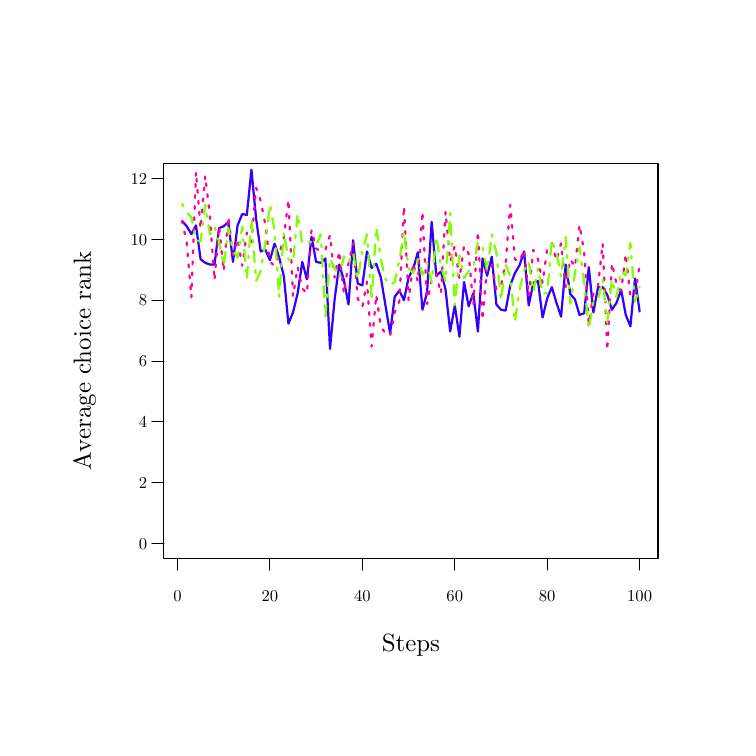
\begin{tikzpicture}[x=1pt,y=1pt]
\definecolor{fillColor}{RGB}{255,255,255}
\path[use as bounding box,fill=fillColor,fill opacity=0.00] (0,0) rectangle (252.94,252.94);
\begin{scope}
\path[clip] ( 49.20, 61.20) rectangle (227.75,203.75);
\definecolor{drawColor}{RGB}{51,0,255}

\path[draw=drawColor,line width= 0.8pt,line join=round,line cap=round] ( 55.81,183.07) --
	( 57.48,181.18) --
	( 59.15,178.35) --
	( 60.82,181.50) --
	( 62.49,169.24) --
	( 64.16,167.98) --
	( 65.83,167.35) --
	( 67.50,167.35) --
	( 69.17,180.55) --
	( 70.84,181.18) --
	( 72.51,182.75) --
	( 74.18,168.30) --
	( 75.85,181.50) --
	( 77.52,185.58) --
	( 79.19,185.27) --
	( 80.86,201.61) --
	( 82.53,184.01) --
	( 84.20,172.07) --
	( 85.87,172.70) --
	( 87.54,168.93) --
	( 89.21,174.90) --
	( 90.88,169.87) --
	( 92.55,163.27) --
	( 94.22,145.99) --
	( 95.89,150.07) --
	( 97.56,156.98) --
	( 99.23,168.30) --
	(100.90,162.01) --
	(102.57,177.41) --
	(104.24,168.30) --
	(105.91,167.98) --
	(107.58,169.55) --
	(109.25,136.87) --
	(110.92,154.78) --
	(112.59,167.35) --
	(114.26,161.70) --
	(115.93,152.90) --
	(117.60,176.15) --
	(119.27,160.44) --
	(120.94,159.81) --
	(122.61,172.07) --
	(124.28,166.10) --
	(125.95,167.67) --
	(127.62,162.64) --
	(129.29,152.58) --
	(130.96,142.53) --
	(132.63,155.73) --
	(134.30,157.93) --
	(135.97,154.47) --
	(137.64,162.64) --
	(139.31,165.78) --
	(140.98,171.75) --
	(142.65,151.01) --
	(144.32,157.30) --
	(145.99,182.75) --
	(147.66,163.27) --
	(149.33,164.84) --
	(151.00,158.24) --
	(152.67,143.16) --
	(154.34,152.58) --
	(156.01,141.27) --
	(157.68,161.07) --
	(159.35,152.27) --
	(161.02,156.98) --
	(162.69,143.16) --
	(164.36,169.55) --
	(166.03,163.27) --
	(167.70,170.18) --
	(169.37,152.90) --
	(171.04,151.01) --
	(172.71,150.70) --
	(174.38,159.81) --
	(176.05,164.21) --
	(177.71,167.04) --
	(179.38,172.07) --
	(181.05,152.58) --
	(182.72,160.76) --
	(184.39,161.38) --
	(186.06,148.19) --
	(187.73,155.10) --
	(189.40,159.18) --
	(191.07,153.53) --
	(192.74,148.50) --
	(194.41,167.35) --
	(196.08,156.67) --
	(197.75,154.78) --
	(199.42,149.13) --
	(201.09,149.76) --
	(202.76,166.41) --
	(204.43,150.07) --
	(206.10,159.18) --
	(207.77,159.18) --
	(209.44,156.36) --
	(211.11,151.01) --
	(212.78,153.53) --
	(214.45,158.24) --
	(216.12,149.13) --
	(217.79,145.04) --
	(219.46,162.33) --
	(221.13,150.38);
\end{scope}
\begin{scope}
\path[clip] (  0.00,  0.00) rectangle (252.94,252.94);
\definecolor{drawColor}{RGB}{0,0,0}

\path[draw=drawColor,line width= 0.4pt,line join=round,line cap=round] ( 54.14, 61.20) -- (221.13, 61.20);

\path[draw=drawColor,line width= 0.4pt,line join=round,line cap=round] ( 54.14, 61.20) -- ( 54.14, 56.92);

\path[draw=drawColor,line width= 0.4pt,line join=round,line cap=round] ( 87.54, 61.20) -- ( 87.54, 56.92);

\path[draw=drawColor,line width= 0.4pt,line join=round,line cap=round] (120.94, 61.20) -- (120.94, 56.92);

\path[draw=drawColor,line width= 0.4pt,line join=round,line cap=round] (154.34, 61.20) -- (154.34, 56.92);

\path[draw=drawColor,line width= 0.4pt,line join=round,line cap=round] (187.73, 61.20) -- (187.73, 56.92);

\path[draw=drawColor,line width= 0.4pt,line join=round,line cap=round] (221.13, 61.20) -- (221.13, 56.92);

\node[text=drawColor,anchor=base,inner sep=0pt, outer sep=0pt, scale=  0.60] at ( 54.14, 45.60) {0};

\node[text=drawColor,anchor=base,inner sep=0pt, outer sep=0pt, scale=  0.60] at ( 87.54, 45.60) {20};

\node[text=drawColor,anchor=base,inner sep=0pt, outer sep=0pt, scale=  0.60] at (120.94, 45.60) {40};

\node[text=drawColor,anchor=base,inner sep=0pt, outer sep=0pt, scale=  0.60] at (154.34, 45.60) {60};

\node[text=drawColor,anchor=base,inner sep=0pt, outer sep=0pt, scale=  0.60] at (187.73, 45.60) {80};

\node[text=drawColor,anchor=base,inner sep=0pt, outer sep=0pt, scale=  0.60] at (221.13, 45.60) {100};

\path[draw=drawColor,line width= 0.4pt,line join=round,line cap=round] ( 49.20, 66.48) -- ( 49.20,198.47);

\path[draw=drawColor,line width= 0.4pt,line join=round,line cap=round] ( 49.20, 66.48) -- ( 44.92, 66.48);

\path[draw=drawColor,line width= 0.4pt,line join=round,line cap=round] ( 49.20, 88.48) -- ( 44.92, 88.48);

\path[draw=drawColor,line width= 0.4pt,line join=round,line cap=round] ( 49.20,110.47) -- ( 44.92,110.47);

\path[draw=drawColor,line width= 0.4pt,line join=round,line cap=round] ( 49.20,132.47) -- ( 44.92,132.47);

\path[draw=drawColor,line width= 0.4pt,line join=round,line cap=round] ( 49.20,154.47) -- ( 44.92,154.47);

\path[draw=drawColor,line width= 0.4pt,line join=round,line cap=round] ( 49.20,176.47) -- ( 44.92,176.47);

\path[draw=drawColor,line width= 0.4pt,line join=round,line cap=round] ( 49.20,198.47) -- ( 44.92,198.47);

\node[text=drawColor,anchor=base east,inner sep=0pt, outer sep=0pt, scale=  0.60] at ( 43.20, 64.41) {0};

\node[text=drawColor,anchor=base east,inner sep=0pt, outer sep=0pt, scale=  0.60] at ( 43.20, 86.41) {2};

\node[text=drawColor,anchor=base east,inner sep=0pt, outer sep=0pt, scale=  0.60] at ( 43.20,108.41) {4};

\node[text=drawColor,anchor=base east,inner sep=0pt, outer sep=0pt, scale=  0.60] at ( 43.20,130.41) {6};

\node[text=drawColor,anchor=base east,inner sep=0pt, outer sep=0pt, scale=  0.60] at ( 43.20,152.40) {8};

\node[text=drawColor,anchor=base east,inner sep=0pt, outer sep=0pt, scale=  0.60] at ( 43.20,174.40) {10};

\node[text=drawColor,anchor=base east,inner sep=0pt, outer sep=0pt, scale=  0.60] at ( 43.20,196.40) {12};

\path[draw=drawColor,line width= 0.4pt,line join=round,line cap=round] ( 49.20, 61.20) --
	(227.75, 61.20) --
	(227.75,203.75) --
	( 49.20,203.75) --
	( 49.20, 61.20);
\end{scope}
\begin{scope}
\path[clip] (  0.00,  0.00) rectangle (252.94,252.94);
\definecolor{drawColor}{RGB}{0,0,0}

\node[text=drawColor,anchor=base,inner sep=0pt, outer sep=0pt, scale=  0.90] at (138.47, 27.60) {Steps};

\node[text=drawColor,rotate= 90.00,anchor=base,inner sep=0pt, outer sep=0pt, scale=  0.90] at ( 22.80,132.47) {Average choice rank};
\end{scope}
\begin{scope}
\path[clip] ( 49.20, 61.20) rectangle (227.75,203.75);
\definecolor{drawColor}{RGB}{255,0,153}

\path[draw=drawColor,line width= 0.8pt,dash pattern=on 1pt off 3pt ,line join=round,line cap=round] ( 55.81,183.16) --
	( 57.48,175.03) --
	( 59.15,155.43) --
	( 60.82,200.86) --
	( 62.49,180.29) --
	( 64.16,199.42) --
	( 65.83,185.08) --
	( 67.50,161.64) --
	( 69.17,181.25) --
	( 70.84,164.99) --
	( 72.51,184.60) --
	( 74.18,170.73) --
	( 75.85,176.47) --
	( 77.52,166.90) --
	( 79.19,178.86) --
	( 80.86,175.51) --
	( 82.53,195.12) --
	( 84.20,190.34) --
	( 85.87,181.73) --
	( 87.54,168.34) --
	( 89.21,166.90) --
	( 90.88,171.21) --
	( 92.55,176.95) --
	( 94.22,190.81) --
	( 95.89,155.90) --
	( 97.56,166.43) --
	( 99.23,158.77) --
	(100.90,156.86) --
	(102.57,179.82) --
	(104.24,173.12) --
	(105.91,172.16) --
	(107.58,172.64) --
	(109.25,177.90) --
	(110.92,162.60) --
	(112.59,172.16) --
	(114.26,156.86) --
	(115.93,167.86) --
	(117.60,175.03) --
	(119.27,154.95) --
	(120.94,152.08) --
	(122.61,161.17) --
	(124.28,137.73) --
	(125.95,156.38) --
	(127.62,144.91) --
	(129.29,142.51) --
	(130.96,141.56) --
	(132.63,150.17) --
	(134.30,153.99) --
	(135.97,188.42) --
	(137.64,154.47) --
	(139.31,167.86) --
	(140.98,161.17) --
	(142.65,186.51) --
	(144.32,153.04) --
	(145.99,162.12) --
	(147.66,164.03) --
	(149.33,156.86) --
	(151.00,186.51) --
	(152.67,168.34) --
	(154.34,174.08) --
	(156.01,162.12) --
	(157.68,174.08) --
	(159.35,171.21) --
	(161.02,152.56) --
	(162.69,179.34) --
	(164.36,147.30) --
	(166.03,166.90) --
	(167.70,167.38) --
	(169.37,158.30) --
	(171.04,159.73) --
	(172.71,167.86) --
	(174.38,188.90) --
	(176.05,169.29) --
	(177.71,168.34) --
	(179.38,172.64) --
	(181.05,155.90) --
	(182.72,172.64) --
	(184.39,169.29) --
	(186.06,160.69) --
	(187.73,173.12) --
	(189.40,175.03) --
	(191.07,168.82) --
	(192.74,175.03) --
	(194.41,159.25) --
	(196.08,169.29) --
	(197.75,166.43) --
	(199.42,181.73) --
	(201.09,171.69) --
	(202.76,145.86) --
	(204.43,156.86) --
	(206.10,159.73) --
	(207.77,175.03) --
	(209.44,136.30) --
	(211.11,167.86) --
	(212.78,160.21) --
	(214.45,157.82) --
	(216.12,171.21) --
	(217.79,155.90) --
	(219.46,156.38) --
	(221.13,167.38);
\definecolor{drawColor}{RGB}{128,255,0}

\path[draw=drawColor,line width= 0.8pt,dash pattern=on 1pt off 3pt on 4pt off 3pt ,line join=round,line cap=round] ( 55.81,189.26) --
	( 57.48,186.19) --
	( 59.15,184.40) --
	( 60.82,176.21) --
	( 62.49,175.70) --
	( 64.16,189.00) --
	( 65.83,178.26) --
	( 67.50,181.07) --
	( 69.17,175.44) --
	( 70.84,167.00) --
	( 72.51,180.56) --
	( 74.18,172.38) --
	( 75.85,169.82) --
	( 77.52,181.07) --
	( 79.19,162.14) --
	( 80.86,183.89) --
	( 82.53,161.38) --
	( 84.20,164.96) --
	( 85.87,175.19) --
	( 87.54,189.00) --
	( 89.21,179.54) --
	( 90.88,155.49) --
	( 92.55,179.03) --
	( 94.22,169.31) --
	( 95.89,168.28) --
	( 97.56,185.68) --
	( 99.23,174.93) --
	(100.90,175.70) --
	(102.57,175.44) --
	(104.24,174.42) --
	(105.91,178.26) --
	(107.58,148.59) --
	(109.25,169.56) --
	(110.92,165.98) --
	(112.59,162.66) --
	(114.26,170.33) --
	(115.93,168.03) --
	(117.60,171.61) --
	(119.27,162.14) --
	(120.94,172.38) --
	(122.61,178.26) --
	(124.28,154.21) --
	(125.95,180.82) --
	(127.62,169.31) --
	(129.29,162.14) --
	(130.96,159.84) --
	(132.63,161.12) --
	(134.30,168.79) --
	(135.97,179.28) --
	(137.64,165.98) --
	(139.31,164.19) --
	(140.98,169.31) --
	(142.65,163.68) --
	(144.32,168.03) --
	(145.99,160.86) --
	(147.66,177.49) --
	(149.33,167.00) --
	(151.00,161.12) --
	(152.67,185.93) --
	(154.34,152.68) --
	(156.01,170.58) --
	(157.68,162.40) --
	(159.35,164.96) --
	(161.02,166.24) --
	(162.69,175.44) --
	(164.36,173.91) --
	(166.03,164.96) --
	(167.70,178.26) --
	(169.37,171.61) --
	(171.04,154.47) --
	(172.71,167.26) --
	(174.38,163.17) --
	(176.05,146.54) --
	(177.71,158.05) --
	(179.38,165.21) --
	(181.05,168.28) --
	(182.72,157.54) --
	(184.39,165.98) --
	(186.06,156.77) --
	(187.73,157.03) --
	(189.40,176.21) --
	(191.07,171.61) --
	(192.74,162.91) --
	(194.41,177.24) --
	(196.08,153.19) --
	(197.75,164.19) --
	(199.42,173.65) --
	(201.09,160.86) --
	(202.76,143.98) --
	(204.43,153.96) --
	(206.10,154.73) --
	(207.77,162.14) --
	(209.44,146.54) --
	(211.11,161.89) --
	(212.78,155.49) --
	(214.45,164.96) --
	(216.12,163.42) --
	(217.79,175.19) --
	(219.46,153.96) --
	(221.13,159.33);
\end{scope}
\end{tikzpicture}
 \\
				(\textbf{a}) Blockwise entropy by cluster & (\textbf{b}) Average choice rank by cluster \\
		\end{tabular} \quad
		\caption{Clustering on choices vs. model parameter estimation (top sub figures: experiment 1, high noise, bottom: experiment 1, low noise)}
		\label{fig:cluse1c3}
\end{figure}


\pagebreak
\subsection{Prison data}

\begin{table}[!htbp] \centering 
	\caption{} 
	\label{} 
	\scriptsize 
	\begin{tabular}{@{\extracolsep{0pt}} llcccccccccc} 
		\toprule
		Groups & Method & Similarity & C & CBC & BBC & E & EB & CC & NMI & ARI & VM \\ 
		\hline \\[-1.8ex] 
		6vs1 & Spectral & EDR &  &  &  & x &  &  & 0.237 (0.000) & 0.020 (0.000) & 0.237 (0.000) \\ 
		& K-Means &  &  &  &  &  & x &  & 0.167 (0.000) & - & 0.166 (0.000) \\ 
		& Spectral & Euclidean &  & x &  &  &  &  & 0.057 (0.000) & 0.036 (0.000) & 0.057 (0.000) \\ 
		& Spectral & EDR &  &  & x &  &  &  & 0.037 (0.000) & 0.034 (0.000) & 0.037 (0.000) \\ 
		& K-Means & Euclidean &  &  &  &  &  & x & 0.023 (0.028) & - & 0.023 (0.028) \\ 
		& K-Means &  & x &  &  &  &  &  & 0.020 (0.022) & - & 0.020 (0.023) \\ 
		& Average &  &  &  &  &  &  &  & 0.068 (0.068) & - & 0.067 (0.068) \\ 
		6vs2 & K-Means &  &  & x &  &  &  &  & 0.289 (0.052) & 0.217 (0.063) & 0.278 (0.055) \\ 
		& K-Means &  &  &  &  & x &  &  & 0.165 (0.000) & 0.083 (0.000) & 0.145 (0.000) \\ 
		& Spectral & Cosine &  &  &  &  & x &  & 0.165 (0.000) & 0.083 (0.000) & 0.145 (0.000) \\ 
		& Ward & Euclidean &  &  & x &  &  &  & 0.072 (0.000) & 0.083 (0.000) & 0.071 (0.000) \\ 
		& K-Means &  & x &  &  &  &  &  & 0.041 (0.022) & - & 0.041 (0.022) \\ 
		& K-Means & Euclidean &  &  &  &  &  & x & 0.028 (0.023) & - & 0.028 (0.023) \\ 
		& Average &  &  &  &  &  &  &  & 0.116 (0.088) & 0.058 (0.081) & 0.110 (0.083) \\ 
		6vs3 & Spectral & warp &  &  &  & x &  &  & 0.205 (0.000) & - & 0.203 (0.000) \\ 
		& K-Means &  &  &  &  &  & x &  & 0.174 (0.000) & - & 0.171 (0.000) \\ 
		& Spectral & warp &  & x &  &  &  &  & 0.116 (0.000) & - & 0.110 (0.000) \\ 
		& Ward & Euclidean &  &  & x &  &  &  & 0.116 (0.000) & - & 0.110 (0.000) \\ 
		& Lavenstein &  & x &  &  &  &  &  & 0.116 (0.000) & - & 0.110 (0.000) \\ 
		& K-Means & Euclidean &  &  &  &  &  & x & 0.110 (0.023) & - & 0.105 (0.022) \\ 
		& Average &  &  &  &  &  &  &  & 0.089 (0.056) & - & 0.086 (0.055) \\ 
		6vs4 & Spectral & EDR &  &  &  & x &  &  & 0.360 (0.000) & 0.227 (0.000) & 0.342 (0.000) \\ 
		& Spectral & Euclidean  &  &  &  &  & x &  & 0.246 (0.000) & 0.229 (0.000) & 0.246 (0,000) \\ 
		& Ward & Euclidean  &  & x &  &  &  &  & 0.105 (0.000) & - & 0.102 (0.000) \\ 
		& Complete & Euclidean  &  &  & x &  &  &  & 0.848 (0.000) & - & 0.080 (0.000) \\ 
		& K-Means & Euclidean  & x &  &  &  &  &  & 0.049 (0.000) & - & 0.049 (0.000) \\ 
		& K-Means & Euclidean  &  &  &  &  &  & x & 0.080 (0.050) & - & 0.079 (0.048) \\ 
		& Average &  &  &  &  &  &  &  & 0.089 (0.088) & - & 0.088 (0.088) \\ 
		6vs9 & Ward  & Euclidean &  &  &  &  & x &  & 0.561 (0.000) & 0.560 (0,000) & 0.560 (0,000) \\ 
		& Spectral & DTW &  &  &  & x &  &  & 0.435 (0.000) & 0.387 (0.000) & 0.432 (0.000) \\ 
		& Spectral & DTW &  & x &  &  &  &  & 0.435 (0.000) & 0.387 (0.000) & 0.432 (0.000) \\ 
		& Spectral & EDR &  &  & x &  &  &  & 0.333 (0.000) & 0.381 (0.000) & 0.333 (0.000) \\ 
		& Spectral & Overlap & x &  &  &  &  &  & 0.111 (0.000) & 0.118 (0.000) & 0.111 (0.000) \\ 
		& K-Means & Euclidean &  &  &  &  &  & x & 0.106 (0.066) & 0.033 (0.054) & 0.094 (0.059) \\ 
		& Average &  &  &  &  &  &  &  & 0.249 (0.167) & 0.202 (0.189) & 0.244 (0.169) \\ 
		\hline \\[-1.8ex] 
	\end{tabular} 
	\label{tab:prison1}
\end{table} 

\begin{table}[!htbp] \centering 
	\caption{} 
	\label{} 
	\scriptsize 
	\begin{tabular}{@{\extracolsep{0pt}} cccccccccccc} 
		\toprule
		Groups & Method & Similarity & C & CBC & BBC & E & EB & CC & NMI & ARI & VM \\ 
		\hline \\[-1.8ex] 
		2vs4 & Spectral & eucsim/rbf &  & x &  &  &  &  & 0.213 (0.000) & 0.007 (0.000) & 0.211 (0.000) \\ 
		& Levenstein &  & x &  &  &  &  &  & 0.213 (0.000) & 0.007 (0.000) & 0.211 (0.000) \\ 
		& Spectral & EDR &  &  &  & x &  &  & 0.132 (0.000) & 0.104 (0.000) & 0.131 (0.000) \\ 
		& Spectral & EDR &  &  & x &  &  &  & 0.054 (0.000) & - & 0.054 (0.000) \\ 
		& Spectral & eblock &  &  &  &  & x &  & 0.018 (0.000) & - & 0.017 (0.000) \\ 
		& K-Means & Euclidean &  &  &  &  &  & x & 0.005 (0.005) & - & 0.005 (0.005) \\ 
		&  &  &  &  &  &  &  &  & 0.042 (0.063) & - & 0.041 (0.063) \\ 
		2vs6 & K-Means &  &  & x &  &  &  &  & 0.3 (0.048) & 0.23 (0.062) & 0.291 (0.510) \\ 
		& K-Means &  &  &  &  & x &  &  & 0.165 (0.000) & 0.083 (0.000) & 0.145 (0.000) \\ 
		& Spectral & Cosine &  &  &  &  & x &  & 0.165 (0.000) & 0.083 (0.000) & 0.145 (0.000) \\ 
		& Ward & Euclidean &  &  & x &  &  &  & 0.072 (0.000) & 0.083 (0.000) & 0.071 (0.000) \\ 
		& K-Means & Euclidean &  &  &  &  &  & x & 0.027 (0.020) & - & 0.027 (0.020) \\ 
		& K-Means &  & x &  &  &  &  &  & 0.023 (0.021) & - & 0.023 (0.021) \\ 
		&  &  &  &  &  &  &  &  & 0.112 (0.090) & 0.057 (0.082) & 0.106 (0.085) \\ 
		2vs9 & Spectral & EDR &  &  &  & x &  &  & 0.382 (0.000) & 0.235 (0.000) & 0.382 (0.000) \\ 
		& Spectral & EDR &  &  & x &  &  &  & 0.232 (0.000) & 0.226 (0.000) & 0.232 (0.000) \\ 
		& Spectral & Cosine &  &  &  &  & x &  & 0.197 (0.000) & 0.008 (0.000) & 0.191 (0.000) \\ 
		& Spectral & eucsim/rbf &  & x &  &  &  &  & 0.134 (0.000) & 0.075 (0.000) & 0.134 (0.000) \\ 
		& K-Means & Euclidean &  &  &  &  &  & x & 0.116 (0.000) & - & 0.105 (0.000) \\ 
		& K-Means &  & x &  &  &  &  &  & 0.111 (0.022) & - & 0.100 (0.020) \\ 
		&  &  &  &  &  &  &  &  & 0.096 (0.074) & - & 0.093 (0.073) \\ 
		\hline \\[-1.8ex] 
	\end{tabular} 
	\label{tab:prison2}
\end{table} 





\end{appendix}

\pagebreak
%----------------------------------------------------------------------------------------------------------
% End Document
%----------------------------------------------------------------------------------------------------------

\end{document}
